\bookpart{推断}{Inference}
\label{part:pgm-inference}

\BookPartGuide{%
模型结构和局部概率函数给定以后，推断要回答边缘概率、条件概率、最可能配置等查询。完整枚举所有配置通常不可行，图模型的价值在于沿局部因子复用中间计算，并明确哪些近似改变了计算对象、哪些近似只引入有限误差。

第~\ref{chap:pgm-elimination}章“基于变量消除的精确推断”先定义证据、查询和待消变量，再用因子乘法、证据约简与边缘化把重复求和整理成桶计算；消元顺序如何产生中间团，是理解推断成本的关键。第~\ref{chap:pgm-junction-tree}章“基于团树传播的精确推断”把这些中间因子保存为可复用的团和消息，通过树结构上的传播与校准支持多次查询，同时说明消息重复计数和分隔集处理。第~\ref{chap:pgm-variational}章“变分推断与确定性近似”把查询转成优化问题：在易处理的分布族中最小化与目标后验的差异，或松弛离散配置约束，误差由近似族、界和证书共同说明。第~\ref{chap:pgm-sampling}章“基于采样的近似推断”用随机样本估计期望和概率，依次讨论拒绝、重要性采样、MCMC、序贯重要性采样与粒子方法，并把有限样本波动、混合和退化与估计精度联系起来。

四种方法不是简单的精度排序。变量消除和团树在给定模型上追求精确答案，但成本由树宽和中间因子大小决定；变分方法用可计算分布换取系统偏差，采样方法保持渐近目标却引入有限样本波动。阅读时应固定查询、证据、输出量和误差口径，再比较各方法复用了哪些局部计算。}

\chapter{基于变量消除的精确推断}
\label{chap:pgm-elimination}

前四章解决的是“怎样表示”一个概率模型：给定图和局部因子，联合分布被写成一组局部函数的乘积。从本章开始进入第二部分，要回答表示之后最自然的问题——模型已经建好，怎样用它回答具体查询？这就是\term{推断}（inference）。设备报警后，维修人员面对的诊断任务通常有两种输出：一种是给出故障的后验概率，回答“有多可能是故障”；另一种是直接选出一组最可能的故障、过热和传感器状态，回答“最可能是什么情形”。这两种输出使用同一组局部因子，区别只在于用什么方式汇总那些没有观测到、也不要求作答的状态。

先看最朴素的做法为什么不够。要计算一个后验概率，原则上可以列出所有变量的完整联合配置，把符合查询和证据的配置权重逐一相加。但对$d$个二元变量，完整配置有$2^d$个：$d=30$时就超过十亿，变量再多便完全不可行。联合分布写成局部因子乘积的意义正在于避免这种指数级的整体枚举——许多局部和与查询变量无关，可以先算一次、再被多个查询配置重复使用。利用局部分解识别并消除这些重复计算，正是精确推断的主要任务。本章从第~\ref{sec:pgm-representations-local-computation}节已经引入的因子组合与消元操作出发，把它发展成完整、可证明正确的算法。

核心想法是逐个处理未知变量，而不是一次处理全部。查询通常只保留部分变量，某个未知变量对答案的全部影响，可以先汇总成一个只依赖剩余变量的更小函数，供后续步骤重复使用。\term{变量消除}（variable elimination, VE）据此逐个收集含有当前变量的因子。本步收集到的这些因子称为当前变量的\term{桶}（bucket）——之所以必须一起处理，是因为它们要使用当前变量的同一个状态，不能各自独立求和。将桶内因子相乘，再以求和、积分或最大化消去该变量，所得新函数便可替换桶内函数，保存它们对剩余变量的共同影响。

本章围绕三个问题展开：其一，为什么这样逐桶替换不会改变最终的查询答案，这需要一个贯穿全章的不变式来证明；其二，不同查询（求概率、求最可能完整配置、求部分变量的最优值）为什么要选用求和或最大化等不同算子，以及这些算子能否交换次序；其三，消元顺序怎样改变中间函数的作用域，从而决定计算量。离散因子以状态组合数表示规模，高斯因子则以矩阵块维度表示规模，两种表示由此产生不同的计算代价。

\section{推断问题与因子运算}
\label{sec:pgm-elimination-factor-operations}

\subsection{查询、证据与消元变量}
\label{sec:pgm-elimination-query-evidence}

在给出算法前，先把一个推断查询涉及的变量角色固定下来，这是后面所有记号的基础。求故障后验时，要固定报警证据，保留故障变量作为查询目标，并把其余未知状态全部汇总掉。一般地，模型的节点集合为$V$，节点$i$对应随机变量$X_i$；已观测节点组成$O\subseteq V$，取值为$\bm{x}_O=\bm{e}$，查询节点组成$Q\subseteq V\setminus O$。剩下既未观测、也不查询的节点称为待消元节点，记为$R=V\setminus(O\cup Q)$——它们的值不是答案，但它们的各种取值都会影响答案，需要被汇总。三个大写集合指定变量角色，$\bm{x}_Q$才是一组查询状态。证据集合用$O$记，以便与图的边集合$E$区分。

以下把模型参数视为已知输入。设共有$m$个非负因子$\psi_a$，其完整乘积具有有限且非零的归一化常数$Z$，联合分布写为
\begin{equation}
  p(\bm{x})=\frac{1}{Z}\prod_{a=1}^{m}\psi_a(\bm{x}_{S_a}),
  \qquad S_a\subseteq V.
  \label{eq:pgm-elimination-factorization}
\end{equation}
有向模型采用局部条件概率作为因子，完整积已归一化，故$Z=1$。无向模型的势需由全局$Z$归一化。这些函数都是当前推断的输入，第~\ref{chap:pgm-parameter-learning}章再讨论如何从数据估计它们。

把证据坐标固定在观测值后，原乘积成为未观测变量上的函数：
\begin{equation}
  F_{\bm{e}}(\bm{x}_{V\setminus O})
  =\left.\prod_{a=1}^{m}\psi_a(\bm{x}_{S_a})
  \right|_{\bm{x}_O=\bm{e}}.
  \label{eq:pgm-elimination-evidence-function}
\end{equation}
先取各变量状态数有限的离散情形。汇总$R$的联合状态得到查询权重，再对$Q$的所有状态归一化：
\begin{equation}
  \begin{aligned}
    g_Q(\bm{x}_Q)
      &=\sum_{\bm{x}_R}F_{\bm{e}}(\bm{x}_Q,\bm{x}_R),\\
    Z_{\bm{e}}&=\sum_{\bm{x}_Q}g_Q(\bm{x}_Q),\\
    p(\bm{x}_Q\mid\bm{e})&=\frac{g_Q(\bm{x}_Q)}{Z_{\bm{e}}}.
  \end{aligned}
  \label{eq:pgm-elimination-marginal-query}
\end{equation}
下标$\bm{x}_R$遍历待消元变量的联合状态。这里值得指出一个在实现上很方便的事实：总权重满足$Z_{\bm{e}}=Zp(\bm{e})$，因此计算条件概率时，无向模型那个麻烦的全局归一化常数$Z$会在分子分母中直接抵消。也就是说，无论模型有没有写出$Z$，推断都可以直接从未归一化的因子乘积出发，最后只做一次归一化。后验比值在$Z_{\bm{e}}>0$的证据事件上有定义；模型赋予观测零概率时，该比值的分母为零，此时条件分布本身没有定义。

连续变量用积分汇总未知坐标。联合密度存在且积分有限时，式~\eqref{eq:pgm-elimination-marginal-query}的积分版本给出边缘条件密度。连续观测处的$p(\bm{e})$表示边缘密度值，比值只在密度有限且为正的观测处使用。形式相同的查询还需配合适当的函数表示，才能解析完成积分。

\subsection{因子乘积}
\label{sec:pgm-elimination-factor-product}

变量消除每一步都在对因子做三种基本操作：相乘、按证据切片、对未知变量求和。这三种操作各自改变因子的不同坐标，后续算法会反复使用它们。

相乘两张因子表时，需要按变量身份及状态含义对齐坐标。\term{作用域}（scope）指定因子的自变量。一次消元先合并相关因子的作用域，再从中去掉本次被消去的变量，余下坐标就是新因子需要保留的输入。若$D_i$是$X_i$的取值集合，作用域为$S$的离散因子是非负函数$\psi_S:\prod_{i\in S}D_i\to[0,\infty)$。存储表时还要记下$S$内变量的排列和状态编码：同一变量可以位于不同表轴上，但相乘时同一个状态必须有相同含义。

两个函数分别使用$A$与$B$中的变量，乘积便使用它们的并集$A\cup B$：
\begin{equation}
  (\psi_A\psi_B)(\bm{x}_{A\cup B})
  =\psi_A(\bm{x}_A)\psi_B(\bm{x}_B).
  \label{eq:pgm-elimination-product}
\end{equation}
对$A\cup B$的一组取值，两因子各读取自己的坐标，其中共享变量取同一状态。例如，$\psi_{\{F,H\}}(f,h)\psi_{\{H,S\}}(h,s)$以$(f,h,s)$为索引；计算$(0,1,0)$时，分别读取前表$(0,1)$与后表$(1,0)$。三个变量均为二元时，两张$4$项表的乘积共有$8$项，新增的坐标来自两表作用域的并集。

因子保存相对权重，其全表求和可以异于$1$。空作用域的因子是标量，也参与完整乘积；条件概率比较中的公共尺度可约去，而证据概率或绝对得分需要这些尺度。乘积还要保留函数的出现次数：两个数值相同的因子仍相乘两次。以下的$\mathcal{F}$因此按多重集合使用。

\subsection{因子约简与边缘化}
\label{sec:pgm-elimination-reduction-marginalization}

观测把一个变量的状态固定后，可以从因子表读取相应切片。把证据代入并从作用域移去固定坐标，称为\term{因子约简}（factor reduction）。报警证据$A=1$将$p(a\mid h,s)$变为$\ell_A(h,s)=p(A=1\mid h,s)$，表示各$(h,s)$状态对该报警的支持权重。结合先验与其他因子、再统一归一化，才能得到这些原因的后验分布。

对状态仍未知的变量，概率查询要汇总其全部取值。\term{边缘化}（marginalization）把这些权重相加，留下其余坐标上的函数：若$i\in S$，则
\begin{equation}
  (\mathop{\textstyle\sum}_{x_i}\psi_S)
    (\bm{x}_{S\setminus\{i\}})
  =\sum_{x_i\in D_i}\psi_S(\bm{x}_{S\setminus\{i\}},x_i).
  \label{eq:pgm-elimination-factor-marginal}
\end{equation}
约简读取已知状态下的切片，边缘化累加未知状态。两种操作都减少自变量数，分别保留观测条件下的权重与未知变量的总贡献。

一个未知变量可能同时出现在多个因子中，这时汇总的次序至关重要：必须让这些因子共享$X_i$的同一个状态。若$X_i$同时出现在$\psi_1(x_i,y)$和$\psi_2(x_i,z)$中，正确做法是先相乘、再对共同的$x_i$求和，所得新因子为
\[
  \sum_{x_i}\psi_1(x_i,y)\psi_2(x_i,z)\text{。}
\]
反过来，若先各自对$x_i$求和再相乘，相当于允许第一张表选定的$x_i$取值与第二张表选定的取值彼此独立、互不相同，这就破坏了“同一个$x_i$”的约束，得到的是另一个量。因此，消元必须先收集所有含$X_i$的因子、把它们乘在一起，再对共同乘积汇总；新函数保留的是这些因子在剩余坐标上的联合影响。这也解释了“桶”为什么要成组处理，而不能逐因子独立求和。

完成非查询变量的边缘化后，查询权重可以统一归一化。中途若用一个与全部自变量无关的正常数缩放因子，最终条件概率的公共尺度仍会抵消，但计算$Z_{\bm{e}}$需记录并补回该常数。逐行归一化的除数随剩余坐标变化，会改变各查询配置的相对权重，因而属于对函数的实质修改。

\section{边缘概率的变量消除算法}
\label{sec:pgm-elimination-sum-product}

这一节用一个可以逐项手算的小模型，看清变量消除究竟省下了什么，再把其中的规则提炼成一般算法。故障后验要把所有非查询状态的权重相加，因此这里使用求和消元。我们先在报警模型上比较完整枚举与局部汇总，找出能够重复使用的子计算，再把相同规则写成一般算法。保留多个查询变量时，汇总规则不变，改变的是输出函数的坐标；连续变量则把求和换成积分，还需选择能够精确保存积分结果的函数表示。

\subsection{从朴素枚举到分配律}
\label{sec:pgm-elimination-distributivity}

沿用报警模型作为可逐项计算的例子：故障$F$、过热$H$、报警$A$和传感器失灵$S$均取$0$或$1$。联合分解为
\begin{equation}
  p(f,h,a,s)=p(f)p(h\mid f)p(s)p(a\mid h,s).
  \label{eq:pgm-elimination-alarm-model}
\end{equation}
有向结构$F\to H\to A\leftarrow S$使两个根节点$F,S$独立。设置$p(F=1)=0.1$、$p(S=1)=0.05$，并取
\[
  p(H=1\mid F=0)=0.1,\qquad
  p(H=1\mid F=1)=0.8.
\]
表~\ref{tab:pgm-elimination-alarm-cpt}给出四种$(h,s)$下的报警概率；二元分布的状态$0$概率都由$1$减去状态$1$概率得到。这组人工参数只用于解释消元步骤。

\begin{table}[htbp]
  \centering
  \begin{tabular}{ccc}
    \toprule
    $h$ & $s$ & $p(A=1\mid h,s)$\\
    \midrule
    $0$ & $0$ & $0.01$\\
    $1$ & $0$ & $0.90$\\
    $0$ & $1$ & $0.70$\\
    $1$ & $1$ & $0.99$\\
    \bottomrule
  \end{tabular}
  \caption{报警模型的人工条件表。每行固定$(h,s)$并列出$p(A=1\mid h,s)$，同一行的不报警概率为$1-p(A=1\mid h,s)$。}
  \label{tab:pgm-elimination-alarm-cpt}
\end{table}

将$A=1$代入报警因子后，故障查询需要累加过热和传感器的全部状态：
\[
  g_F(f)=\sum_h\sum_s p(f)p(h\mid f)p(s)\ell_A(h,s).
\]
直接枚举对每个$f$访问全部$(h,s)$，共需访问$8$个三元配置。仔细观察会发现，其中$p(s)\ell_A(h,s)$这部分完全不含$f$：无论查询的是$f=0$还是$f=1$，它都要被计算同样一遍。让两种故障状态共享这部分结果，就能避免重复。利用乘法对加法的分配律（先对与当前变量无关的因子求和，再乘回相关因子，结果不变），先对$s$汇总与它相关的两个函数：
\begin{equation}
  g_F(f)
  =p(f)\sum_h p(h\mid f)
    \underbrace{\sum_s p(s)\ell_A(h,s)}_{\tau_S(h)}.
  \label{eq:pgm-elimination-alarm-reorder}
\end{equation}
所得$\tau_S(h)$替换$p(s)$与$\ell_A(h,s)$，对每种$h$计算一次，供所有$f$使用。下一步将$p(h\mid f)\tau_S(h)$对$h$求和，生成$f$上的函数。图~\ref{fig:pgm-elimination-alarm-buckets}将每步输入与输出的坐标分别画出。

\begin{figure}[htbp]
  \centering
  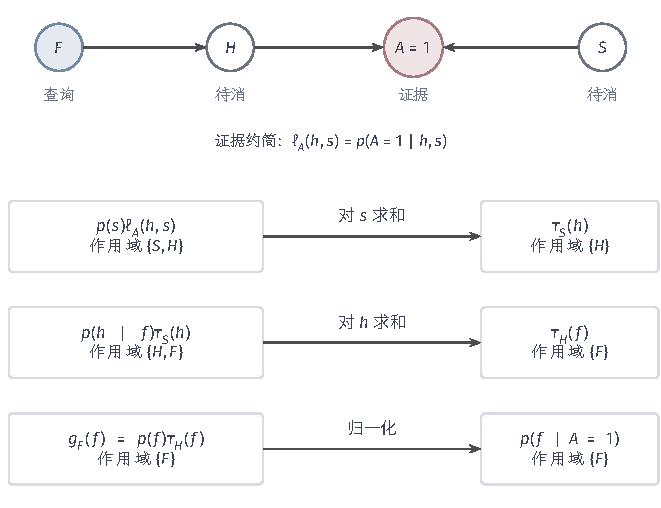
\includegraphics[width=112.000mm]{figures/09-probabilistic-graphical-models/02-inference/tikz/pgm-elimination-alarm-buckets/figure.pdf}
  \caption{故障后验查询的两步消元。上方有向图中，蓝色$F$为查询变量，红色$A=1$为证据，灰边空心的$H,S$为待消变量。下方先从$p(s)\ell_A(h,s)$求和得到$\tau_S(h)$，再从$p(h\mid f)\tau_S(h)$求和得到$\tau_H(f)$。每步输出的作用域只保留尚未消去的坐标；最终将$g_F(f)=p(f)\tau_H(f)$按$f$归一化，得到$p(f\mid A=1)$。}
  \label{fig:pgm-elimination-alarm-buckets}
\end{figure}

这种重排让后续故障状态复用同一局部汇总，每个$s,h$状态仍以原权重参与求和，所以代数结果与完整枚举相同——这正是“消除”而非“近似”的含义：它只改变求和的组织次序，不改变任何一项的贡献。能省多少取决于输出函数的作用域：新表只涉及剩余变量，若一桶包含几乎全部剩余变量，形成的新表仍可能很大。选择消元顺序的目的，就是控制这类中间函数的坐标数和状态组合数，这是第~\ref{sec:pgm-elimination-complexity}节的主题。

\subsection{变量消除算法}
\label{sec:pgm-elimination-ve-algorithm}

一般因子分解也按同一方式替换局部乘积。证据约简后的初始因子多重集合记为$\mathcal{F}^{(0)}$，顺序$\pi=(i_1,\ldots,i_k)$将待消元集合$R$的每个节点列出恰好一次。第$t$步收集全部含$X_{i_t}$的因子：
\[
  \mathcal{B}_t
  =\{\psi\in\mathcal{F}^{(t-1)}:
      i_t\in\operatorname{scope}(\psi)\}.
\]
$\operatorname{scope}(\psi)$给出函数的作用域。前面所说的变量的桶，现在由多重集合$\mathcal{B}_t$准确记录，其中的函数需要共同参与本步求和。令$U_t$为它们作用域的并集，去掉当前变量后的集合为$N_t=U_t\setminus\{i_t\}$，局部更新写为
\begin{equation}
  \begin{aligned}
    \phi_t(\bm{x}_{U_t})&=\prod_{\psi\in\mathcal{B}_t}\psi,\\
    \tau_t(\bm{x}_{N_t})&=\sum_{x_{i_t}}\phi_t(\bm{x}_{U_t}).
  \end{aligned}
  \label{eq:pgm-elimination-local-sum}
\end{equation}
计算$\phi_t$时，先按式~\eqref{eq:pgm-elimination-product}对齐每个函数的坐标。桶外函数不含$X_{i_t}$，从本步求和提出后仍留在当前集合中。

\begin{algorithm}[离散边缘概率的变量消除]
  \label{alg:pgm-elimination-marginal}
  \begin{algorithmic}[1]
    \Require 取有限非负值的离散因子$\{\psi_a\}$，证据$\bm{x}_O=\bm{e}$，查询集$Q$
    \Require $R=V\setminus(O\cup Q)$的排列$\pi=(i_1,\ldots,i_k)$
    \Ensure 查询因子$g_Q$及$Z_{\bm{e}}>0$时的条件分布
    \State 将证据代入各因子，得到$\mathcal{F}^{(0)}$；保留标量因子
    \State 对未出现在任何作用域中的未观测变量，加入其恒为$1$的一元因子
    \For{$t=1,\ldots,k$}
      \State 收集$\mathcal{B}_t$，令$U_t$为其作用域的并集
      \State 对齐坐标并求乘积$\phi_t=\prod_{\psi\in\mathcal{B}_t}\psi$
      \State 对$x_{i_t}$求和，得到$\tau_t(\bm{x}_{U_t\setminus\{i_t\}})$
      \State $\mathcal{F}^{(t)}\gets
        (\mathcal{F}^{(t-1)}\setminus\mathcal{B}_t)\cup\{\tau_t\}$
    \EndFor
    \State 在查询取值空间上计算$g_Q=\prod_{\psi\in\mathcal{F}^{(k)}}\psi$
    \State 计算$Z_{\bm{e}}=\sum_{\bm{x}_Q}g_Q(\bm{x}_Q)$
    \If{$Z_{\bm{e}}=0$}
      \State 返回证据与模型不相容，条件分布未定义
    \Else
      \State 返回$g_Q$、$Z_{\bm{e}}$及$g_Q/Z_{\bm{e}}$
    \EndIf
  \end{algorithmic}
\end{algorithm}

算法~\ref{alg:pgm-elimination-marginal}按出现次数移除桶内函数并加入新因子。若某个未观测变量未进入任何函数，加入恒为$1$的一元因子后，它的求和仍贡献状态数。$R=\varnothing$时没有消元步骤，$Q=\varnothing$时最终乘积是证据权重标量$Z_{\bm{e}}$。边缘查询输出汇总后的函数，各个已消变量的状态都参与了累加，因此输出无需配置回溯。

报警例的数值虽然小，却能完整展示算法每一步。报警查询从$p(f)$、$p(h\mid f)$、$p(s)$和$\ell_A(h,s)$四因子开始。先处理$S$桶：$p(s)$与$\ell_A(h,s)$相乘后对$s$求和，两种$h$下的新函数值分别为
\begin{equation}
  \begin{aligned}
    \tau_S(0)&=0.95\times0.01+0.05\times0.70=0.0445,\\
    \tau_S(1)&=0.95\times0.90+0.05\times0.99=0.9045.
  \end{aligned}
  \label{eq:pgm-elimination-alarm-s}
\end{equation}
用$\tau_S(h)$替换$S$桶后，当前集合为$\{p(f),p(h\mid f),\tau_S(h)\}$。接着将含$H$的两个函数相乘并求和，得到
\begin{equation}
  \begin{aligned}
    \tau_H(0)&=0.9\times0.0445+0.1\times0.9045=0.1305,\\
    \tau_H(1)&=0.2\times0.0445+0.8\times0.9045=0.7325.
  \end{aligned}
  \label{eq:pgm-elimination-alarm-h}
\end{equation}
余下$p(f)$与$\tau_H(f)$相乘，给出$g_F(0)=0.11745$、$g_F(1)=0.07325$，总权重为$0.19070$。原有向联合积的$Z=1$，因此此值也是证据概率$p(A=1)$。把故障状态$1$的权重除以总权重，得到
\begin{equation}
  p(F=1\mid A=1)
  =\frac{0.07325}{0.19070}
  \approx0.384111.
  \label{eq:pgm-elimination-alarm-posterior}
\end{equation}
报警使故障概率从$0.1$升至约$0.384$。无故障过热、传感器失灵以及小概率误报也能解释报警，它们的概率都进入求和分母；保留这些解释使后验仍低于$1$。

这个顺序只产生$\tau_S(h)$、$\tau_H(f)$两张一元表。变量较多的模型可先按消元顺序分桶。对一个输入因子，先看它的作用域是否含有待消元节点：若含有，就交给顺序中最早的那个节点；若只含查询节点，就放入最终查询因子池，留到所有桶处理结束后再相乘。空作用域的标量因子也保留在最终池中，使绝对证据权重不丢失。

每步新函数也按同一规则交接：仍含尚未消去的节点时，送往其中最早的后续桶；只剩查询坐标或成为标量时，放入最终池。当前报警查询中，$p(f)$从开始便留在最终池，$\tau_S(h)$送往$H$桶，最后生成的$\tau_H(f)$才汇入最终池。两者相乘得到$g_F(f)$，与算法~\ref{alg:pgm-elimination-marginal}保留当前因子集合再取积的做法一致。这种收集、合并、汇总的组织方式对应Dechter的桶消除算法\scite{pgm-elimination-dechter1999}

\subsection{多变量查询}
\label{sec:pgm-elimination-multivariate-query}

联合查询故障与传感器状态时，保留$Q=\{F,S\}$，仅消去$H$。所需结果使用$(f,s)$共同索引：
\begin{equation}
  g_{F,S}(f,s)
  =p(f)p(s)\sum_h p(h\mid f)\ell_A(h,s).
  \label{eq:pgm-elimination-joint-query}
\end{equation}
以$f=s=0$为例，先汇总两种过热状态，得到
\[
  \begin{aligned}
    g_{F,S}(0,0)
    &=0.9\times0.95\times(0.9\times0.01+0.1\times0.90)\\
    &=0.084645.
  \end{aligned}
\]
对其余三种$(f,s)$执行相同求和，即得到表~\ref{tab:pgm-elimination-joint-query}。

\begin{table}[htbp]
  \centering
  \begin{tabular}{ccc}
    \toprule
    $f$ & $g_{F,S}(f,0)$ & $g_{F,S}(f,1)$\\
    \midrule
    $0$ & $0.084645$ & $0.032805$\\
    $1$ & $0.068590$ & $0.004660$\\
    \bottomrule
  \end{tabular}
  \caption{报警证据下的未归一化$(F,S)$联合权重。四项共用归一化常数$0.19070$，得到$p(f,s\mid A=1)$；若各行分别归一化，则得到给定$f$后的传感器条件分布。}
  \label{tab:pgm-elimination-joint-query}
\end{table}

四项总权重为$0.19070$，各行之和是$g_F(f)$，各列之和是$g_S(s)$。虽然$F,S$观测前独立，报警后的两种原因相互影响：一种解释的后验权重会改变另一种解释的相对可信度。联合表保留了这种关系，两个一元后验的乘积一般给不出它。显式联合输出还有自身的存储代价；保留的查询变量越多，即使各消元桶较小，最后的联合表也可能很大。

\subsection{连续变量的边缘消除}
\label{sec:pgm-elimination-gaussian}

连续变量（如温度、测量值）的推断思路完全一样：先把涉及同一变量的因子相乘，再对它积分；不含当前坐标的因子可以提出积分号，非负可测性允许按Tonelli定理交换积分次序。条件密度还要求总积分有限且为正。但离散情形里“对有限状态求和”总是可以逐项完成并精确保存，连续情形则多了一个表示问题：积分后的函数未必还能用有限个参数精确表达。例如对任意形状的势做积分，结果可能是一个没有简单闭式的函数。因此能否解析消元，取决于因子的函数形式。高斯分布的二次指数形式恰好具有一个好性质：高斯函数相乘、以及在合法条件下积分，结果仍然是高斯二次指数。它因此提供了一个可以完整、精确计算的连续例子，本节就以它说明连续消元的参数如何更新。

高斯核的自变量记为$\bm{x}\in\mathbb{R}^{q}$。将其写成\term{规范形式}（canonical form），以二次项、一次项及常数项系数保存函数，便于相乘时合并参数：
\begin{equation}
  \psi(\bm{x})
  =\exp\!\left\{-\frac12\bm{x}^{\top}\bm{J}\bm{x}
                  +\bm{h}^{\top}\bm{x}+c\right\}
  \text{。}
  \label{eq:pgm-elimination-gaussian-canonical}
\end{equation}
参数$\bm{J}\in\mathbb{R}^{q\times q}$对称，$\bm{h}\in\mathbb{R}^{q}$，$c$为标量。对均值$\bm{\mu}$、协方差$\bm{\Sigma}$的非退化高斯密度，\term{精度矩阵}（precision matrix）$\bm{J}=\bm{\Sigma}^{-1}$以逆协方差表示二次项，$\bm{h}=\bm{J}\bm{\mu}$，归一化常数进入$c$。局部因子可以在部分方向没有二次约束；所有因子组合后的联合精度要求正定，使完整高斯核可归一化。以下用同样的三参数形式保存局部函数，但只对可归一化的完整核将其二次项矩阵解释为概率分布的精度。

规范形式相乘会将指数相加，因此对齐坐标后分别累加$\bm{J}$、$\bm{h}$和$c$即可。不在某因子作用域内的坐标补零，与离散表相乘时扩展坐标的操作对应。吸收证据仍是代入，不过观测坐标还会通过交叉二次项改变保留坐标的一次项。将当前函数的坐标分为保留块$\bm{x}_A$和观测块$\bm{x}_O=\bm{e}$，我们先把代入后的指数完整写出：
\[
  \begin{aligned}
    &-\frac12\bm{x}_A^{\top}\bm{J}_{A,A}\bm{x}_A
      -\frac12\bm{x}_A^{\top}\bm{J}_{A,O}\bm{e}
      -\frac12\bm{e}^{\top}\bm{J}_{O,A}\bm{x}_A\\
    &\quad-\frac12\bm{e}^{\top}\bm{J}_{O,O}\bm{e}
      +\bm{h}_A^{\top}\bm{x}_A+\bm{h}_O^{\top}\bm{e}+c
      \text{。}
  \end{aligned}
\]
由于$\bm{J}$对称，两个交叉项是相同的标量，合起来为$-\bm{x}_A^{\top}\bm{J}_{A,O}\bm{e}$。它对$\bm{x}_A$是一次项；只含$\bm{e}$的部分则与保留坐标无关，进入常数项。按这三类项读取系数，得到约简后的参数：
\[
  \begin{aligned}
    \bm{J}'&=\bm{J}_{A,A},\\
    \bm{h}'&=\bm{h}_A-\bm{J}_{A,O}\bm{e},\\
    c'&=c+\bm{h}_O^{\top}\bm{e}
       -\frac12\bm{e}^{\top}\bm{J}_{O,O}\bm{e}
       \text{。}
  \end{aligned}
\]
这组参数保存固定$\bm{x}_O$后的函数，未观测变量仍全部保留。接下来积分消元才汇总未知坐标的贡献。

一次积分先收集所有含待消变量的因子，将桶积写成式~\eqref{eq:pgm-elimination-gaussian-canonical}。作用域分为待消块$B$和保留块$A$，令$\bm{y}=\bm{x}_B\in\mathbb{R}^{b}$、$\bm{z}=\bm{x}_A\in\mathbb{R}^{a}$，相应参数为
\[
  \bm{J}=
  \begin{pmatrix}
    \bm{J}_{B,B}&\bm{J}_{B,A}\\
    \bm{J}_{A,B}&\bm{J}_{A,A}
  \end{pmatrix},
  \qquad
  \bm{h}=
  \begin{pmatrix}\bm{h}_B\\\bm{h}_A\end{pmatrix}
  \text{。}
\]
这里的$\bm{J}$和$\bm{h}$只来自当前桶。为区分局部函数与完整当前乘积，另以$T$表示当前尚未消去的全部节点，以$\bm{K}$和$\bm{\eta}$分别表示完整乘积的二次项和一次项参数。令$C=T\setminus B$为积分后全部剩余坐标；本桶的保留集$A$只是$C$的子集。桶外函数不含$\bm{y}$，因此它们不向$B,B$块贡献二次项，完整矩阵满足$\bm{K}_{B,B}=\bm{J}_{B,B}$。同样，$\bm{K}_{B,C}$由$\bm{J}_{B,A}$在$C$中其余坐标处补零得到。

关于$\bm{y}$的积分使用正定主块$\bm{J}_{B,B}\succ0$。非退化联合高斯模型的完整精度正定；证据约简后取相应主块仍然正定。若完整当前精度$\bm{K}\succ0$，它的主块$\bm{K}_{B,B}$正定，所以上述相等关系保证本桶满足积分条件。下面还会证明，完整边缘核的更新矩阵继续正定，因而这一条件可以逐步保持。这里要求正定的是被积分的主块；整个局部桶矩阵$\bm{J}$可以在其它方向没有约束。

为了计算一次积分，我们先从指数中提取含$\bm{y}$的项。利用$\bm{J}_{A,B}=\bm{J}_{B,A}^{\top}$合并交叉项，得到
\[
  -\frac12\bm{y}^{\top}\bm{J}_{B,B}\bm{y}
  +\bm{y}^{\top}(\bm{h}_B-\bm{J}_{B,A}\bm{z})
  \text{。}
\]
未写入这一行的保留项为$-\bm{z}^{\top}\bm{J}_{A,A}\bm{z}/2+\bm{h}_A^{\top}\bm{z}+c$。这些项与$\bm{y}$无关，所以它们对应的指数函数可以提出积分号，但仍须乘在积分结果上。将线性系数记为$\bm{u}(\bm{z})=\bm{h}_B-\bm{J}_{B,A}\bm{z}$。对$\bm{y}$配方，可以分离需要积分的高斯核与保留的$\bm{z}$函数：
\begin{equation}
  \begin{aligned}
    &-\frac12
      \bigl(\bm{y}-\bm{J}_{B,B}^{-1}\bm{u}\bigr)^{\top}
      \bm{J}_{B,B}
      \bigl(\bm{y}-\bm{J}_{B,B}^{-1}\bm{u}\bigr)\\
    &\hspace{2em}
      +\frac12\bm{u}^{\top}\bm{J}_{B,B}^{-1}\bm{u}
      \text{。}
  \end{aligned}
  \label{eq:pgm-elimination-complete-square}
\end{equation}
固定$\bm{z}$后，第一项中的中心$\bm{J}_{B,B}^{-1}\bm{u}$也固定。平移积分变量不会改变Lebesgue测度，因此这部分高斯核的积分为$(2\pi)^{b/2}|\bm{J}_{B,B}|^{-1/2}$，与核中心无关。余项$\bm{u}^{\top}\bm{J}_{B,B}^{-1}\bm{u}/2$仍依赖保留变量，不能并入一个与$\bm{z}$无关的尺度后丢弃。

要看清被消块怎样改变保留块，先把这一余项按$\bm{z}$展开：
\[
  \begin{aligned}
    \frac12\bm{u}^{\top}\bm{J}_{B,B}^{-1}\bm{u}
    ={}&\frac12\bm{h}_B^{\top}\bm{J}_{B,B}^{-1}\bm{h}_B\\
       &-\bm{z}^{\top}\bm{J}_{A,B}\bm{J}_{B,B}^{-1}\bm{h}_B\\
       &+\frac12\bm{z}^{\top}\bm{J}_{A,B}
          \bm{J}_{B,B}^{-1}\bm{J}_{B,A}\bm{z}
          \text{。}
  \end{aligned}
\]
第一行不含$\bm{z}$，第二行是$\bm{z}$的一次项，第三行是二次项。把第三行与原来的$-\bm{z}^{\top}\bm{J}_{A,A}\bm{z}/2$合并，就得到更新后二次系数中的减项；把第二行与$\bm{h}_A^{\top}\bm{z}$合并，就得到更新后的一次系数。积分产生的正数乘因子也要保留：将其写入指数，增加的常数是$(b/2)\log(2\pi)-(1/2)\log|\bm{J}_{B,B}|$。重新收集三类系数，所得参数为
\begin{equation}
  \begin{aligned}
    \bm{J}'&=\bm{J}_{A,A}
      -\bm{J}_{A,B}\bm{J}_{B,B}^{-1}\bm{J}_{B,A},\\
    \bm{h}'&=\bm{h}_A
      -\bm{J}_{A,B}\bm{J}_{B,B}^{-1}\bm{h}_B,\\
    c'&=c+\frac12\bm{h}_B^{\top}\bm{J}_{B,B}^{-1}\bm{h}_B\\
      &\quad+\frac b2\log(2\pi)-\frac12\log|\bm{J}_{B,B}|
      \text{。}
  \end{aligned}
  \label{eq:pgm-elimination-schur}
\end{equation}
积分输出仍写成$\exp\{-\bm{z}^{\top}\bm{J}'\bm{z}/2+\bm{h}'^{\top}\bm{z}+c'\}$。更新矩阵$\bm{J}'$是$\bm{J}_{B,B}$在$\bm{J}$中的\term{Schur补}（Schur complement），其中减去的矩阵项保存了被消块对保留块的影响。若当前桶已经包含完整联合核，这个Schur补就是该联合核的边缘精度。取完整高斯分布的边缘时，协方差表示直接保留相应主块；精度表示则使用这个Schur补。两种更新各对应自己的参数化。

一般消元步骤还存在桶外函数，局部更新矩阵$\bm{J}'$须先与那些函数的二次系数相加，才能成为完整边缘核的精度。具体地，把$\bm{J}'$按$A\subseteq C$补零嵌入全部剩余坐标$C$，记为$\widetilde{\bm{J}}'$；将桶外函数的二次系数和记为$\bm{K}_{\mathrm{out}}$，则完整边缘精度为$\bm{K}'=\widetilde{\bm{J}}'+\bm{K}_{\mathrm{out}}$。由完整当前矩阵的分块也能直接算出同一个结果：
\[
  \begin{aligned}
    \bm{K}'&=\bm{K}_{C,C}
       -\bm{K}_{C,B}\bm{K}_{B,B}^{-1}\bm{K}_{B,C},\\
    \bm{\eta}'&=\bm{\eta}_C
       -\bm{K}_{C,B}\bm{K}_{B,B}^{-1}\bm{\eta}_B
       \text{。}
  \end{aligned}
\]
这里$\bm{K}_{C,C}$已经含有桶外二次项，而$\bm{K}_{B,B}$与$\bm{K}_{B,C}$仍完全来自桶内函数。因此，直接更新完整矩阵与先更新桶、再乘桶外函数，保存的是同一个边缘函数。

完整当前精度正定还保证完整Schur补$\bm{K}'$正定。对任意非零的保留坐标向量$\bm{v}$，选取$\bm{y}=-\bm{K}_{B,B}^{-1}\bm{K}_{B,C}\bm{v}$，其联合二次型为
\[
  \begin{pmatrix}\bm{y}\\\bm{v}\end{pmatrix}^{\top}
  \bm{K}
  \begin{pmatrix}\bm{y}\\\bm{v}\end{pmatrix}
  =\bm{v}^{\top}\bm{K}'\bm{v}>0
  \text{。}
\]
等号由代入选定的$\bm{y}$并合并交叉项得到；严格大于零则来自$\bm{K}\succ0$以及联合向量非零。对每个$\bm{v}\ne\bm{0}$都成立，正好说明$\bm{K}'\succ0$。这就把当前完整核的正定性传到下一次消元所用的完整核。

这个论证使用完整联合矩阵。局部桶输出尚需与其它函数组合，本身可以在部分方向没有约束。例如，桶积$\exp\{-(y-z)^2/2\}$的被消主块为$1$，积分消去$y$后只剩常数$\sqrt{2\pi}$，局部$\bm{J}'=0$。若桶外还有$\exp\{-z^2/2\}$，相乘后的完整输出才是可归一化的一维高斯核，其完整剩余精度为$1$。为了报告所请求的边缘分布，消去所有非查询变量后，还要将剩余因子组合成完整查询核，再从它的参数读取查询均值和协方差。将这些参数记为$\bm{J}_Q$、$\bm{h}_Q$和$c_Q$，则$\bm{J}_Q\succ0$，均值为$\bm{J}_Q^{-1}\bm{h}_Q$，协方差为$\bm{J}_Q^{-1}$。

均值计算呈现相同的块消元结构。对完整当前核，规范参数与均值满足$\bm{K}\bm{\mu}=\bm{\eta}$。为了消去均值的$B$块，我们把两个块方程分别写出：
\[
  \begin{aligned}
    \bm{K}_{B,B}\bm{\mu}_B
      +\bm{K}_{B,C}\bm{\mu}_C&=\bm{\eta}_B,\\
    \bm{K}_{C,B}\bm{\mu}_B
      +\bm{K}_{C,C}\bm{\mu}_C&=\bm{\eta}_C
      \text{。}
  \end{aligned}
\]
第一行给出$\bm{\mu}_B=\bm{K}_{B,B}^{-1}(\bm{\eta}_B-\bm{K}_{B,C}\bm{\mu}_C)$。把它代入第二行，再将含$\bm{\mu}_C$的项合并到左侧，得到
\[
  \begin{aligned}
    &\bm{K}_{C,B}\bm{K}_{B,B}^{-1}
      (\bm{\eta}_B-\bm{K}_{B,C}\bm{\mu}_C)
      +\bm{K}_{C,C}\bm{\mu}_C
      =\bm{\eta}_C,\\
    &\bigl(\bm{K}_{C,C}
      -\bm{K}_{C,B}\bm{K}_{B,B}^{-1}\bm{K}_{B,C}\bigr)
      \bm{\mu}_C
      =\bm{\eta}_C-\bm{K}_{C,B}\bm{K}_{B,B}^{-1}\bm{\eta}_B
      \text{。}
  \end{aligned}
\]
括号中的矩阵就是$\bm{K}'$，右侧就是$\bm{\eta}'$，所以剩余均值满足$\bm{K}'\bm{\mu}_C=\bm{\eta}'$。若把完整核的两个坐标块记为$B,A$，并沿用最初的$\bm{J}$和$\bm{h}$表示其参数，同一过程就是$\bm{J}\bm{\mu}=\bm{h}$经块消元得到$\bm{J}'\bm{\mu}_A=\bm{h}'$。概率边缘化和线性方程消元由此共用Schur补。

概率计算还需保存$c'$中的积分常数。只求均值时，块方程无需知道核在整个空间上的积分；求证据权重时，却必须累积每次积分贡献的总量。尤其是$(2\pi)^{b/2}|\bm{J}_{B,B}|^{-1/2}$随被消方向的曲率而变，它记录同一中心附近的权重在这些方向上积累了多少。把这一因子及配方产生的常数一并存入$c'$，才能保留原函数的积分质量。Lauritzen的教材系统介绍这种高斯消元关系\scite{pgm-lauritzen1996}。

\begin{example}[一个二维高斯核的积分]
  \label{ex:pgm-elimination-gaussian-numeric}
  以$\bm{x}=(x_1,x_2)^{\top}$的二次核演示一次更新，设置
  \[
    \bm{J}=\begin{pmatrix}2&-1\\-1&2\end{pmatrix},
    \qquad
    \bm{h}=\begin{pmatrix}1\\0\end{pmatrix},
    \qquad c=0
    \text{。}
  \]
  $\bm{J}$的特征值为$1,3$，完整核因而可归一化。积分消去$x_1$，使用$\bm{J}_{B,B}=2$、$\bm{J}_{B,A}=-1$，式~\eqref{eq:pgm-elimination-schur}给出
  \[
    \bm{J}'=\frac32,\qquad \bm{h}'=\frac12,\qquad
    c'=\frac14+\frac12\log\pi
    \text{。}
  \]
  将这三个参数代回一维核，积分输出为
  \[
    \tau(x_2)=\sqrt{\pi}\exp\!\left\{
      \frac14-\frac34x_2^2+\frac12x_2\right\}
      \text{。}
  \]
  对一维输出配方时，指数变为$-(3/4)(x_2-1/3)^2+1/3$。其中二次项对应方差$2/3$，中心为$1/3$，所以归一化后的边缘分布为$x_2\sim\mathcal{N}(1/3,2/3)$。若还需要这个核的总权重，可以继续积分，得到
  \[
    \int_{\mathbb{R}}\tau(x_2)\,\mathrm{d}x_2
    =\sqrt{\pi}\,e^{1/3}\sqrt{\frac{4\pi}{3}}
    =\frac{2\pi}{\sqrt{3}}e^{1/3}
    \text{。}
  \]
  这里$\sqrt{\pi}$和配方后留下的常数共同决定绝对权重，归一化成概率密度时才被统一除去。

  也可从原联合核计算均值和协方差，以独立核对边缘结果：
  \[
    \bm{J}^{-1}=\frac13
      \begin{pmatrix}2&1\\1&2\end{pmatrix},
    \qquad
    \bm{J}^{-1}\bm{h}=
      \begin{pmatrix}2/3\\1/3\end{pmatrix}
      \text{。}
  \]
  所得联合均值的第二项为$1/3$，协方差第二主块为$2/3$，与积分结果相同。仅取原精度的$\bm{J}_{2,2}=2$会对应方差$1/2$，与正确的边缘方差不同；Schur补中的$1/2$修正项恰好保留了$x_1$的影响。
\end{example}

解析更新依靠二次指数函数在乘法和积分下的闭包性。含离散潜变量时，各离散配置下的高斯经求和通常成为高斯混合，分量数还可能随消元增加；非二次势则需另行分析积分是否仍属于二次指数形式。数值求积或将混合压缩成单高斯，是针对这些情形另引入的近似。

\section{MPE与MAP的变量消除算法}
\label{sec:pgm-elimination-max-product}

前述查询求的是各状态的概率，本节换求使权重最大的一组状态。关键区别在于如何处理那些未要求作答的变量：若要给出全部未知变量的一个完整解释，就应让它们一起取到使联合权重最大的那一组值（MPE）；若只关心其中一部分目标变量，就应先把其余变量的各种取值概率汇总（求和）到每个目标候选上，再比较目标状态（边缘MAP）。前者可以纯用最大化逐桶消元，但要额外保存每步的选择才能恢复完整配置；后者在同一计算里混用求和与最大化，两阶段的先后顺序一般不能颠倒。本节先处理较简单的MPE。

\subsection{MPE变量消除}
\label{sec:pgm-elimination-mpe}

诊断还可以要求给出一组最有可能的完整解释。\term{最可能解释}（most probable explanation, MPE）在全部非证据变量的联合状态中比较后验权重，每个候选是一组相容的完整配置。令$U=V\setminus O$，目标为
\begin{equation}
  \begin{aligned}
    \bm{x}_U^\star
    &\in\argmax_{\bm{x}_U}p(\bm{x}_U\mid\bm{e})\\
    &=\argmax_{\bm{x}_U}F_{\bm{e}}(\bm{x}_U).
  \end{aligned}
  \label{eq:pgm-elimination-mpe-objective}
\end{equation}
候选配置共用正常数$Z_{\bm{e}}$，因此可直接比较未归一化的$F_{\bm{e}}$寻找最优配置。报告该配置的后验概率时，再用$Z_{\bm{e}}$归一化其权重。

局部最大化使用非负权重的分配关系：与$x_i$无关的乘数可提出最大化算子，
\[
  \max_{x_i}\{\rho(\bm{z})\phi(x_i,\bm{z})\}
  =\rho(\bm{z})\max_{x_i}\phi(x_i,\bm{z}),
  \qquad \rho(\bm{z})\geq0.
\]
沿用VE的收集和替换操作，把桶内求和换成最大化即可得到最优权重。但最大化消元比求和多一个负担：求和只需知道累加后的数值，最大化若只记下“最大是多少”，事后却无法知道这个最大值是在当前变量取哪个状态时取得的。要恢复完整配置，每一步都必须额外保存取得最大值时的选择，因此还需\term{回溯表}（backpointer table）：对剩余变量的每组配置，记录当前变量的一个最优取值。局部输出和记录分别为
\begin{equation}
  \begin{aligned}
    \tau_t(\bm{x}_{N_t})
      &=\max_{x_{i_t}}\phi_t(x_{i_t},\bm{x}_{N_t}),\\
    b_t(\bm{x}_{N_t})
      &\in\argmax_{x_{i_t}}\phi_t(x_{i_t},\bm{x}_{N_t}).
  \end{aligned}
  \label{eq:pgm-elimination-max-backpointer}
\end{equation}
多个状态并列时，可按约定顺序选取一个并写入回溯表，由此恢复一个最优配置。若输出需要全部最优配置，则保存全部并列选择，回溯输出的数量也可能很大。

\begin{algorithm}[MPE消元及配置回溯]
  \label{alg:pgm-elimination-mpe}
  \begin{algorithmic}[1]
    \Require 约简后的非负因子$\mathcal{F}^{(0)}$及$U$的排列$\pi$
    \Require 各变量取值有限，$Z_{\bm{e}}>0$，每个变量有对应作用域
    \Ensure 最优配置$\bm{x}_U^\star$及未归一化得分$v^\star$
    \For{$t=1,\ldots,|U|$}
      \State 收集含$X_{i_t}$的因子，形成局部乘积$\phi_t$
      \State 令$N_t=\operatorname{scope}(\phi_t)\setminus\{i_t\}$
      \State 按式~\eqref{eq:pgm-elimination-max-backpointer}计算$\tau_t$和$b_t$
      \State 用$\tau_t$替换桶内因子，并保存$(i_t,N_t,b_t)$
    \EndFor
    \State 将剩余标量因子相乘，得到$v^\star$
    \For{$t=|U|,\ldots,1$}
      \State $x_{i_t}^\star\gets b_t(\bm{x}_{N_t}^\star)$
    \EndFor
    \State 返回$\bm{x}_U^\star$和$v^\star$
  \end{algorithmic}
\end{algorithm}

第$t$步的$N_t$只含当时尚未消去的变量，它们在顺序中晚于$i_t$。按逆序恢复时，这些变量已有取值，能够索引$b_t$并确定$x_{i_t}$。最后一个变量的回溯表以空配置为索引，从它开始逐步查表，即可得到完整配置。

报警模型也可逐桶计算MPE。按$S,H,F$消元，先比较每种$h$下传感器两状态的权重：
\[
  \begin{aligned}
    \tau_S^{\max}(0)&=\max\{0.0095,0.0350\}=0.0350,\\
    \tau_S^{\max}(1)&=\max\{0.8550,0.0495\}=0.8550.
  \end{aligned}
\]
取最大值的状态记录为$b_S(0)=1$、$b_S(1)=0$：$H=0$时失灵传感器的报警权重较大，$H=1$时正常传感器的权重较大。当前尚未确定$H$，所以表中保留两种后续状态各自的选择。

对$H$最大化时，$f=0$下的两候选为$0.9\times0.0350=0.0315$与$0.1\times0.8550=0.0855$，记录$\tau_H^{\max}(0)=0.0855$、$b_H(0)=1$。$f=1$下比较$0.2\times0.0350=0.0070$与$0.8\times0.8550=0.6840$，记录$\tau_H^{\max}(1)=0.6840$、$b_H(1)=1$。最后结合故障先验，比较
\[
  \begin{aligned}
    p(F=0)\tau_H^{\max}(0)&=0.07695,\\
    p(F=1)\tau_H^{\max}(1)&=0.06840.
  \end{aligned}
\]
两候选中$f^\star=0$的权重较大。逆序用$b_H(0)$得到$h^\star=1$，再用$b_S(1)$得到$s^\star=0$，完整解释为$(F,H,S)=(0,1,0)$。代入原因子积，其联合证据权重是$0.9\times0.1\times0.95\times0.9=0.07695$，与最大化结果一致；除以证据概率，后验为约$0.403513$。

模型为无故障但过热的状态赋予正概率，因而$(0,1,0)$是合法候选。它的后验约为$0.404$，表示所有完整候选中最大的单项概率，余下候选仍有总概率。$\tau_t^{\max}$保存最佳完成配置的权重，边缘概率则汇总全部完成配置，两种函数有不同的含义。

算法~\ref{alg:pgm-elimination-mpe}使用有限离散状态，保证每桶可枚举并达到最大值。连续变量不能再依靠有限枚举得到这一保证：某些函数只有上确界，没有任何状态取得它；即使最大值存在，局部求解器也未必找到全局最优状态。因此，连续版本还需每次最大值存在且局部优化精确。

高斯核提供了能够精确完成局部最大化的例子。对固定的后续变量$\bm{z}$，配方式~\eqref{eq:pgm-elimination-complete-square}中的负二次项至多为零，并恰在
\[
  \bm{y}^\star(\bm{z})
  =\bm{J}_{B,B}^{-1}(\bm{h}_B-\bm{J}_{B,A}\bm{z})
\]
处取零。回溯不再保存有限个状态索引，而是保存这个关于后续变量的仿射函数；恢复$\bm{z}$后，代入即可得到$\bm{y}^\star$。在最优中心处，平方项消失，只剩配方余项和原来的$\bm{z}$项。因此二次项与一次项仍按Schur补更新，常数项为$c+\bm{h}_B^\top\bm{J}_{B,B}^{-1}\bm{h}_B/2$，没有积分产生的$(b/2)\log(2\pi)-(1/2)\log|\bm{J}_{B,B}|$。积分累加核中心周围的全部质量，最大化只读取中心的最高值，这解释了两种常数更新的差别。

连续情形还须区分密度的众数与坐标无关的概率陈述。作可逆可微换元$Y=T(X)$时，新密度为$p_Y(y)=p_X(T^{-1}(y))\left|\mathrm{d}T^{-1}(y)/\mathrm{d}y\right|$。非线性换元的Jacobian可能随位置改变，因而密度最高点不一定映为新密度的最高点。例如$X\sim\mathcal{N}(0,1)$在$x=0$处取密度最大值，而$Y=\exp X$的对数密度为
\[
  \log p_Y(y)
  =-\frac12(\log y+1)^2+\frac12-\frac12\log(2\pi),
  \qquad y>0.
\]
该式在$y=\exp(-1)$处最大，异于原众数映出的$\exp(0)=1$。因此连续最优解释应按指定坐标和基准测度下的密度众数理解，不能只凭可逆换元就沿用众数位置。

\subsection{MAP变量消除}
\label{sec:pgm-elimination-map}

现在考虑只对一部分目标变量求最优的情形，这在诊断中很常见：我们也许只想知道是否故障，至于过热、传感器这些中间环节的具体组合并不要求给出，只希望把它们的可能性都计入每个故障候选。若诊断只选择故障状态，过热与传感器的各种解释需先汇总到每个故障候选中。\term{边缘最大后验推断}（marginal maximum a posteriori inference, marginal MAP）据此寻找部分目标变量的联合后验众数：对其它未观测变量求和，再比较目标状态。记目标集合为$M\subseteq V\setminus O$，待求和集合为$R=V\setminus(O\cup M)$，目标写为
\begin{equation}
  \bm{x}_M^\star
  \in\argmax_{\bm{x}_M}\sum_{\bm{x}_R}
       F_{\bm{e}}(\bm{x}_M,\bm{x}_R).
  \label{eq:pgm-elimination-map-objective}
\end{equation}
取$M=V\setminus O$、$R=\varnothing$，这一目标就退化为MPE。部分文献也以“MAP”指MPE，本节用“边缘MAP”指明同时含求和与最大化的查询。

边缘MAP同时含求和与最大化，立刻会遇到一个算法问题：这两种算子能不能随意交换次序？答案是一般不能，而且交换后得到的是另一个含义不同的量，数值往往更大。先用一个可逐项复算的无证据例子看清差别。第~\ref{sec:pgm-representations-local-computation}节已用二元表说明两种算子不能任意交换。这里保留一个可逐项复算的无证据例子，进一步从数值差别推出一般上界与等号条件，再据此安排MAP消元与回溯。表~\ref{tab:pgm-elimination-map-counterexample}设置二元目标$X$和二元未知变量$Y$的联合分布，用它比较两种次序。

\begin{table}[htbp]
  \centering
  \begin{tabular}{cccc}
    \toprule
    $x$ & $p(x,Y=0)$ & $p(x,Y=1)$ & $\sum_y p(x,y)$\\
    \midrule
    $0$ & $0.40$ & $0.05$ & $0.45$\\
    $1$ & $0.28$ & $0.27$ & $0.55$\\
    \bottomrule
  \end{tabular}
  \caption{不同查询及算子次序的数值反例。边缘MAP对每行求和后取较大行，选择$X=1$；MPE取最大单元格$(X,Y)=(0,0)$，两者给出不同的$X$状态。}
  \label{tab:pgm-elimination-map-counterexample}
\end{table}

先累加每个$x$行再取最大值，得到$\max_x\sum_y p(x,y)=0.55$，故边缘MAP选择$x^\star=1$。先对每列选$x$则给出$\sum_y\max_x p(x,y)=0.40+0.27=0.67$：它在$Y=0$列选$X=0$，在$Y=1$列选$X=1$，把不同目标状态的收益合并。这个值没有对应的固定$x$候选。原表中最大的完整配置是$(0,0)$，故MPE的$X$分量也异于边缘MAP答案。

两种次序的比较可推广至任意有限非负表$f(x,y)$：
\begin{equation}
  \max_x\sum_y f(x,y)
  \leq \sum_y\max_x f(x,y).
  \label{eq:pgm-elimination-sum-max-bound}
\end{equation}
取左侧的一个最优$x^\star$，每列都有$f(x^\star,y)\leq\max_x f(x,y)$，相加便得到不等式。等号要求存在同一个$x^\star$同时最大化所有列：各列差值非负，总差为零恰要求每列差都为零。反例表的两列各选不同的$x$，所以这里严格小于。

对任意非负因子，先消去全部求和变量$R$、再最大化全部目标变量$M$，可保证边缘MAP目标保持原样。第一阶段沿用算法~\ref{alg:pgm-elimination-marginal}的桶求和，保留其输出因子分解即可，无需先物化完整$M$表或归一化。第二阶段采用算法~\ref{alg:pgm-elimination-mpe}的最大化与回溯，只恢复$M$中的目标状态；已求和的$R$贡献保留在函数中。

特定函数结构可以放宽两阶段次序。例如目标分解为$f(x)g(y,\bm{z})$时，非负性使$\max_x$与$\sum_y$能在两个独立部分交换；所有列共用最优$x$等数值结构也可使等号成立。仅根据任意非负因子的作用域安排通用消元时，采用两阶段顺序保留正确性保证。其它换序有时给出式~\eqref{eq:pgm-elimination-sum-max-bound}的上界，与精确MAP目标不同。

这里需要区分两种换序依据。若一个目标变量的当前桶已经不含任何尚未求和的变量，则它的最大化只作用于目标变量上的局部函数，可以与桶外的求和交换；这种保证只使用作用域，对同一作用域内任意非负函数都成立。若桶仍含待求和坐标，却因当前数值恰好共用最优状态而换序，则还依赖特定参数等式。本章把前一类称为结构有效的消元顺序，默认采用的先求和、后最大化顺序是其中容易检查的一类。Park与Darwiche的定理5进一步说明：对这类标准结构有效顺序，总能找到一条宽度相同、把目标变量排在最后的顺序。这使两阶段顺序足以刻画该结构消元族可达到的最小宽度；它不排除利用特殊函数数值或其它算法获得不同的计算收益\scite{pgm-elimination-park2004}

报警例若只选$F$，先对$S,H$求和后比较$g_F(0)=0.11745$和$g_F(1)=0.07325$，取$F=0$。若同时选择$(F,S)$，先消$H$得到表~\ref{tab:pgm-elimination-joint-query}，再对$F$取最大：$s=0$时保留$0.084645$、记录$b_F(0)=0$，$s=1$时保留$0.032805$、记录$b_F(1)=0$。最后最大化$S$取$s^\star=0$，回溯恢复$f^\star=0$。输出只有目标$(F,S)$，$H$的两种状态已在第一阶段汇总。

报警例的目标答案恰与MPE相应分量一致，而前面的二元表给出了不一致的例子。查询角色因此同时影响输出和可用顺序；固定某些变量必须先求和后，稀疏输入图也可能产生很大的中间函数。

\section{算法分析}
\label{sec:pgm-elimination-analysis}

前面给出了算法并在小例子上验证了结果，还需证明它对任意合法输入都给出正确答案。关键在于说明：把桶内因子相乘后消去一个变量、用更小的新因子替换它们，为何不改变最终查询的答案。为此采用每步更新后都成立的关系（称为不变式）：每消去一个变量，就把它的全部贡献准确汇总进剩余函数。下面先用同类消元的不变式证明答案保持，再以实际作用域分析消元顺序和函数表示带来的成本，最后回到有限精度实现，检查数值尺度、矩阵条件与可复用信息是否仍满足要求。

\subsection{算法正确性}
\label{sec:pgm-elimination-correctness}

多步局部替换的正确性可以用当前乘积的含义来证明：每消去一个变量，就把它的全部贡献汇总进剩余函数。记已消节点为$I_t=\{i_1,\ldots,i_t\}$，初始$I_0=\varnothing$，第$t$步后的乘积为$P^{(t)}=\prod_{\psi\in\mathcal{F}^{(t)}}\psi$。如果每一步的当前乘积都等于原函数对已消变量的聚合结果，那么最后留下的函数就具有所需查询的含义。这种在每步更新后都保持成立的关系，称为算法的不变式。

报警例中的聚合是有限求和，高斯例中的聚合是积分。两者都先把与当前变量无关的乘数提出，再汇总使用该变量的桶积。为了说明这个证明也适用于非高斯的非负函数，下面将积分的基准测度一并写明：有限离散状态采用计数测度时，积分就是逐项求和；欧氏坐标采用Lebesgue测度时，积分就是前面高斯计算所用的连续积分。这里需要沿用的是非负函数可以交换积分次序的条件，而不要求函数始终具有二次指数形式。

积分还要区分每步能否产生有限因子，以及完整函数能否归一化。前者要求局部积分输出在剩余坐标上几乎处处有限，使它可以作为后续步骤的输入；后者要求完整函数的总质量有限且为正，才能得到概率密度。局部输出有限不能代替总质量检查，两项条件分别服务于算法更新与概率解释。纯最大化则有另一项要求：每个局部最优值必须有限，并且能够由某个候选状态达到，才能为配置回溯记录实际选择。下面分别给出求和、积分与纯最大化的不变式。

\begin{theorem}[同类消元的不变式]
  \label{thm:pgm-elimination-invariant}
  设$U=V\setminus O$为有限非观测节点集，$X_i$的状态空间为$\mathcal{X}_i$。对$A\subseteq U$记$\mathcal{X}_A=\prod_{i\in A}\mathcal{X}_i$，空指标集采用单点空间。令$\pi=(i_1,\ldots,i_k)$为$U$中互异节点的消元序列，并令$I_0=\varnothing$、$I_t=\{i_1,\ldots,i_t\}$。初始因子多重集合$\mathcal{F}^{(0)}$为有限多重集合，其中各因子均取有限非负值，其乘积为$F_{\bm{e}}$。

  第$t$步收集全部含$X_{i_t}$的因子，记为$\mathcal{B}_t=\{\psi\in\mathcal{F}^{(t-1)}:i_t\in\operatorname{scope}(\psi)\}$。桶积为$\phi_t=\prod_{\psi\in\mathcal{B}_t}\psi$，消去当前变量后保留的坐标集合为$N_t=(\bigcup_{\psi\in\mathcal{B}_t}\operatorname{scope}(\psi))\setminus\{i_t\}$。以对$X_{i_t}$精确求和、积分或最大化所得的新因子替换$\mathcal{B}_t$，并保留所有标量因子。记$\mathcal{F}^{(t)}$为更新后的因子多重集合，$P^{(t)}=\prod_{\psi\in\mathcal{F}^{(t)}}\psi$。

  若每个变量的状态空间有限非空，则对每个$t=0,\ldots,k$，求和消元满足
  \[
    P^{(t)}(\bm{x}_{(V\setminus O)\setminus I_t})
    =\sum_{\bm{x}_{I_t}}F_{\bm{e}}(\bm{x}_{V\setminus O}).
  \]

  对积分消元，设每个$(\mathcal{X}_i,\mathcal{A}_i)$带有$\sigma$有限基准测度$\mu_i$，各因子非负可测。对$A\subseteq U$记$\mu_A=\bigotimes_{i\in A}\mu_i$，空指标集采用单位测度。要求对每个$t=1,\ldots,k$，局部输出在$\mu_{N_t}$几乎处处的$\bm{x}_{N_t}$有限，其中局部输出由下式计算：
  \[
    \tau_t(\bm{x}_{N_t})
      =\int_{\mathcal{X}_{i_t}}
         \phi_t(x_{i_t},\bm{x}_{N_t})\,\mathrm{d}\mu_{i_t}(x_{i_t}).
  \]
  局部积分为无穷的例外集测度为零，在该集合上可以把输出统一指定为$0$，作为后续计算所用的有限非负可测版本。这个版本与局部积分几乎处处相同。此时对每个$t=0,\ldots,k$，以下积分消元等式对$\mu_{U\setminus I_t}$几乎处处的剩余配置成立：
  \[
    P^{(t)}(\bm{x}_{(V\setminus O)\setminus I_t})
    =\int_{\mathcal{X}_{I_t}}
       F_{\bm{e}}(\bm{x}_{V\setminus O})\,
       \mathrm{d}\mu_{I_t}(\bm{x}_{I_t}).
  \]
  若要将$F_{\bm e}$归一化为概率密度，还须有
  \[
    0<Z_{\bm e}\mathrel{:=}
      \int_{\mathcal{X}_U}F_{\bm e}(\bm{x}_U)\,
      \mathrm{d}\mu_U(\bm{x}_U)<\infty.
  \]

  对纯最大化消元，设各变量状态空间非空。还要求对每个$t=1,\ldots,k$及每个$\bm{x}_{N_t}\in\mathcal{X}_{N_t}$，局部最大值有限且有候选状态达到该值，即
  \[
    \varnothing\neq
    \argmax_{x_{i_t}\in\mathcal{X}_{i_t}}
      \phi_t(x_{i_t},\bm{x}_{N_t}),
    \qquad
    \tau_t^{\max}(\bm{x}_{N_t})
      \mathrel{:=}\max_{x_{i_t}\in\mathcal{X}_{i_t}}
        \phi_t(x_{i_t},\bm{x}_{N_t})<\infty.
  \]
  此时对每个$t=0,\ldots,k$及每个剩余配置，均有
  \[
    P^{(t)}(\bm{x}_{(V\setminus O)\setminus I_t})
    =\max_{\bm{x}_{I_t}\in\mathcal{X}_{I_t}}
       F_{\bm{e}}(\bm{x}_{V\setminus O}).
  \]
\end{theorem}

\begin{proof}
  初始未消去任何变量，$P^{(0)}=F_{\bm{e}}$，满足目标等式。设不变式在第$t-1$步成立，将当前函数分成桶外乘积$\rho_t$和桶积$\phi_t$，即$P^{(t-1)}=\rho_t\phi_t$。桶已包含全部使用$X_{i_t}$的函数，故$\rho_t$不含$x_{i_t}$。求和消元的本步更新满足
  \[
    \begin{aligned}
      P^{(t)}
      &=\rho_t\sum_{x_{i_t}}\phi_t\\
      &=\sum_{x_{i_t}}P^{(t-1)}\\
      &=\sum_{x_{i_t}}\sum_{\bm{x}_{I_{t-1}}}F_{\bm{e}}
       =\sum_{\bm{x}_{I_t}}F_{\bm{e}}.
    \end{aligned}
  \]
  第一行把桶积换为局部求和输出；第二行用分配律将桶外乘积并入本步求和；第三行用归纳假设并合并有限求和。所得等式正是第$t$步的不变式。

  积分版本使用同样的桶内、桶外分解。采用定理中指定的有限版本后，桶外乘积$\rho_t$是有限非负乘数，可以提出关于$x_{i_t}$的积分号。局部积分与新因子在$\mu_{N_t}$几乎处处相同，因此在剩余全部坐标上也几乎处处给出相同的乘积。为说明这一点，记局部例外集为$E_t\subseteq\mathcal{X}_{N_t}$。补入其它未消坐标后，其例外配置组成$E_t$与这些坐标空间的乘积。由于各基准测度均为$\sigma$有限，可以将附加坐标空间写成可数个有限测度集合的并。在每一片上，该乘积集合的测度都是零；取可数并后，例外集合在全部剩余坐标上的乘积测度仍为零。

  还需把前一步几乎处处成立的归纳假设放入本步积分。前一步等式的例外集位于$\mathcal{X}_{U\setminus I_{t-1}}$，其中仍含当前坐标$x_{i_t}$。对例外集的示性函数使用Tonelli定理，可知除$\mu_{U\setminus I_t}$的一个零测集外，每个剩余配置对应的$x_{i_t}$截面都是$\mu_{i_t}$零测集。在这样的剩余配置上，前一步的两个函数关于$x_{i_t}$几乎处处相同，故其积分相同。于是本步的几乎处处等式为
  \[
    \begin{aligned}
      P^{(t)}
      &=\rho_t\int_{\mathcal{X}_{i_t}}
          \phi_t\,\mathrm{d}\mu_{i_t}\\
      &=\int_{\mathcal{X}_{i_t}}
          P^{(t-1)}\,\mathrm{d}\mu_{i_t}\\
      &=\int_{\mathcal{X}_{i_t}}
          \left(\int_{\mathcal{X}_{I_{t-1}}}
            F_{\bm e}\,\mathrm{d}\mu_{I_{t-1}}\right)
          \mathrm{d}\mu_{i_t}\\
      &=\int_{\mathcal{X}_{I_t}}
          F_{\bm e}\,\mathrm{d}\mu_{I_t}.
    \end{aligned}
  \]
  最后一行由因子非负可测及Tonelli定理得到，它允许将这两个积分合并为对已消坐标的乘积积分。本步只需合并局部输出的零测例外和前一步归纳假设产生的截面例外；二者在当前剩余空间中的有限并仍为零测集。逐步重复这一论证，有限次更新的每个阶段都只排除有限个零测例外集，便得到积分不变式。局部输出有限的条件同时保证更新后的乘积在该阶段几乎处处有限。

  纯最大化则利用$\rho_t\geq0$，将$\rho_t\max_{x_{i_t}}\phi_t$写为$\max_{x_{i_t}}(\rho_t\phi_t)$。代入归纳假设后，先对先前已消变量取最大值，再对$x_{i_t}$取最大值，就等于对两组变量的联合配置取最大值。定理要求每个局部最优值都有限且能达到，使这一合并既保留数值，也能选出实现该数值的状态。$\rho_t=0$时两侧都为零，所以证明使用非负性即可。
\end{proof}

边缘查询消去$I_k=R$后，不变式给出最终乘积$P^{(k)}=g_Q$，用$Z_{\bm{e}}$归一化即得到后验。对积分查询，这个等式按相应基准测度几乎处处成立；正且有限的$Z_{\bm e}$使归一化后的函数具有总质量$1$。MPE消去全部$U$后，剩余标量为$v^\star=\max_{\bm{x}_U}F_{\bm{e}}$。

MPE回溯还需恢复达到该值的配置。后续变量取值已确定时，选取$b_t(\bm{x}_{N_t}^\star)$会使本步桶积等于$\tau_t(\bm{x}_{N_t}^\star)$。结合桶外函数，消元前后的乘积在这一扩展配置上相同。由最终标量逆序重复该扩展，得到$F_{\bm{e}}(\bm{x}_U^\star)=v^\star$，同时验证最优得分和所输出配置。

边缘MAP的不变式需要保留两个算子的嵌套次序。第一阶段对$R$逐个求和，当前乘积仍为$P^{(t)}=\sum_{\bm{x}_{I_t}}F_{\bm{e}}$。待全部$R$汇总后，记第二阶段已最大化的目标节点为$J_s\subseteq M$，则
\begin{equation}
  P^{(|R|+s)}
  =\max_{\bm{x}_{J_s}}\sum_{\bm{x}_R}F_{\bm{e}}.
  \label{eq:pgm-elimination-map-invariant}
\end{equation}
第二阶段在已边缘化的目标函数上应用纯最大化不变式。$J_s=M$时得到边缘MAP最优得分，逆序查最大化阶段的回溯表恢复目标配置。若改为交错执行，局部替换保持的是实际顺序对应的嵌套表达式，它是否与MAP目标相同还取决于算子可交换条件。

数学上的精确等式，在浮点实现中仍可能产生误差。浮点加法的舍入使结合顺序影响结果，长乘积可能下溢，病态矩阵求解还会放大输入误差。有限表的完整汇总和高斯解析积分在实数代数中保持等式，计算机结果却可能有舍入差异，近乎并列的候选还可能交换排名。下面的实现段将说明相应的尺度控制与矩阵检查。

\subsection{消元顺序与计算复杂度}
\label{sec:pgm-elimination-complexity}

同一个查询可以采用许多合法的消元顺序，它们给出完全相同的答案，中间付出的代价却可能相差很大；因此在正确性之外，选择顺序是变量消除的主要工程问题。本节建立衡量代价的图论工具（原始关系图、填充边、诱导宽度、树宽），再给出代价界和实用的选点启发式。报警后按$S,H$消元时，依次处理$\{S,H\}$和$\{H,F\}$两个二元桶；先消$H$时，$p(h\mid f)\ell_A(h,s)$使用$F,H,S$三变量，再生成$(f,s)$上的函数。输入因子数相同，首桶访问的状态数不同，因此成本分析要从作用域并集开始。

五节点二元星形图使差距更明显，如图~\ref{fig:pgm-elimination-order-cost}。先消叶节点时，每桶至多含一个叶与中心，访问至多$4$项；先消中心时，桶含五变量，访问$32$项并留下四叶共同函数。两种顺序的最终标量相同，所需中间表规模不同。
\begin{figure*}[htbp]
  \centering
  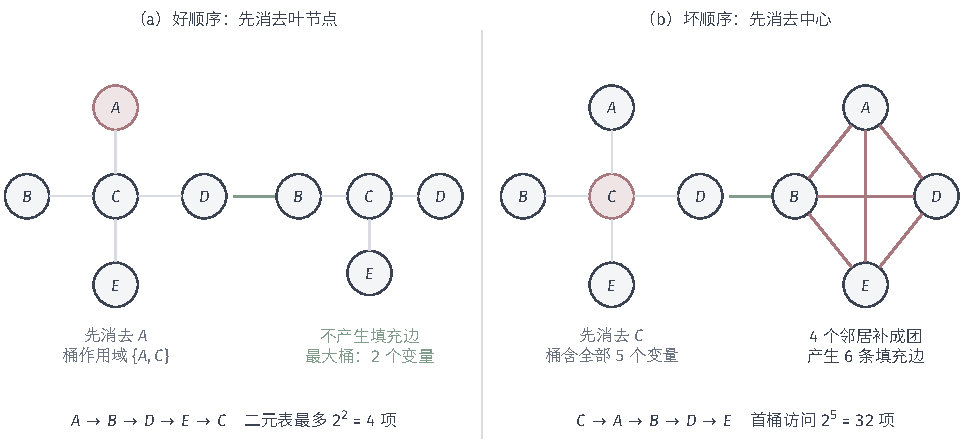
\includegraphics[width=163.153mm]{figures/09-probabilistic-graphical-models/02-inference/tikz/pgm-elimination-order-cost/figure.pdf}
  \caption{五节点二元星形图的两种消元顺序。（a）先消叶节点，每桶至多两个变量且没有填充边；（b）先消中心，首桶枚举$2^5=32$个配置，四个剩余邻居被补成团。红色节点是本步待消变量，红边是新填充边。两边比较稠密表算法的结构代价，最终数值答案保持相同。}
  \label{fig:pgm-elimination-order-cost}
\end{figure*}

要在真正计算函数值之前就预测每一步的表有多大，可以只根据“哪些变量同属一个因子”画出一张辅助图。构造\term{原始关系图}（primal graph）：把每个当前因子的输入节点两两相连，以图邻接记录同一局部函数中的共同坐标。证据代入后，按剩余实际作用域建图；有向条件表的家庭先形成团，再去掉已固定坐标。这个构造保留因子输入，所得图可以异于原DAG骨架。

有了原始关系图，就能直观地看到一次消元对结构的改变。

当前图中节点$i$的邻居记为$N(i)$。桶积使用$\{i\}\cup N(i)$，消去$i$后输出的作用域为$N(i)$，因此将这些剩余节点两两相连并删除$i$。其中新增的边称为\term{填充边}（fill edge），表示新函数的潜在共同作用域；特定参数仍可能使输出抵消或进一步分解。把该顺序产生的填充边全部保留，得到\term{诱导图}（induced graph）。

消元把内部变量的贡献保存到邻域函数。例如先消$H$，$\sum_h p(h\mid f)\ell_A(h,s)$仍以$f,s$为坐标，填充边$F-S$记录这个输出范围。对每组邻域状态，新表保存桶中子问题的完整汇总，后续直接读取它即可。图的填充说明需要保存哪些坐标，函数值说明每组坐标的数值贡献。

\begin{definition}[诱导宽度与树宽]
  \label{def:pgm-elimination-treewidth}
  对无向交互图$\mathcal{G}$的一条完整消元顺序$\pi$，令$N_t$为消去第$t$个节点之前、已经加入前面填充边后的剩余邻居集合。该顺序的\term{诱导宽度}（induced width）是
  \[
    w(\pi)=\max_t|N_t|.
  \]
  图的\term{树宽}（treewidth）定义为所有完整消元顺序中的最小诱导宽度：
  \[
    \operatorname{tw}(\mathcal{G})=\min_\pi w(\pi).
  \]
  宽度不包含本步被消去的节点，所以最大桶作用域的大小为$w(\pi)+1$。
\end{definition}

树宽给出能够达到的最小剩余邻域上界。森林可逐个消叶；含至少一条边时，其树宽为$1$。$d$节点完全图的首节点总有$d-1$个邻居，故树宽为$d-1$。这两个例子说明，节点数之外还需考虑局部作用域的重叠和可选顺序。

每个离散桶需访问多少状态，由变量基数共同决定。记$r_i=|D_i|$，定义作用域状态数
\[
  D(A)=\prod_{i\in A}r_i,\qquad D(\varnothing)=1.
\]
$D(A)$统计状态组合，集合$A$则指定变量。第$t$桶有$c_t$个因子，合并作用域$U_t=\{i_t\}\cup N_t$；稠密对齐、相乘及汇总使用$O(c_tD(U_t))$次标量操作，输出有$D(N_t)$项。完整保存乘积$\phi_t$需另有$D(U_t)$项工作存储。也可枚举每组$\bm{x}_{N_t}$，在$x_{i_t}$轴累加或取最大，把新增工作表缩至$D(N_t)$项；输入及其它未处理函数仍同时占用空间。

所有状态数至多$r$、输入因子数$m=O(d)$时，宽度$w$的完整顺序给出总运算上界
\begin{equation}
  T=O(d\,r^{w+1}).
  \label{eq:pgm-elimination-discrete-time}
\end{equation}
这个总界可以由各桶的代价逐项相加得到。宽度为$w$意味着$|U_t|\leq w+1$，所以每桶的状态数$D(U_t)\leq r^{w+1}$。每个因子只在首个收集它的桶中消耗，每步再产生一个新因子；即使计入孤立变量补入的单位因子，总处理出现次数仍为$\sum_t c_t=O(m+d)$。因此
\[
  \sum_t c_tD(U_t)
  \leq r^{w+1}\sum_t c_t
  =O((m+d)r^{w+1}).
\]
在$m=O(d)$条件下便得到式~\eqref{eq:pgm-elimination-discrete-time}；去掉这一假设时，上式的$d$相应换为$m+d$。此处按标量运算单位成本计，精确有理数位数的增长另属位复杂度。完整物化桶积的峰值为$O(r^{w+1})$，全部新因子及MPE回溯表可由$O(d\,r^w)$上界，实际同时存活部分可能较小。总空间还包括原输入，因而需分别报告输入、临时乘积及保留输出。

边缘查询只消去$R$，保留$Q$。若显式输出完整查询联合表，最后还需$D(Q)$项。设消元阶段的最大$|N_t|$为$w_R$，无消元步骤时取$w_R=0$。消元桶的状态数至多$r^{w_R+1}$，最终查询表则有$D(Q)\leq r^{|Q|}$项。为了用同一个指数上界同时容纳这两种计算，令$\bar w+1$至少等于$w_R+1$和$|Q|$，即将输出规模纳入指标：
\[
  \bar w=\max\{w_R,|Q|-1,0\}.
\]
式中的$|Q|-1$来自输出指数$|Q|$与宽度指数$\bar w+1$的对应，并不表示查询变量少算一个。$Q=\varnothing$时，输出仍是单项标量，$D(Q)=1$；无消元或空查询时再与$0$取最大，避免使用负宽度。在同一基数条件下，消元与最终表乘积的总时间上界为$O((m+d)r^{\bar w+1})$：前一部分沿用逐桶计数，后一部分在每组查询配置上读取全部剩余因子，其处理次数也不超过$O(m+d)$。输出空间为$D(Q)$项。分析显式输出时，也可预先把$Q$补成团并安排在顺序末尾。普通树宽在全部节点的顺序中优化，此查询则要求保留$Q$，两者的候选顺序集合不同。

两种常用启发式通过当前诱导图选择下一变量。\term{最小度启发式}（min-degree）取剩余邻居最少的节点，控制当前桶的变量数；\term{最小填充启发式}（min-fill）取邻居之间缺边最少的节点，试图减少后续填充。每步补边后重新计算这些指标，才能反映当前函数作用域。局部指标可给出可用顺序，但一般不保证全局最优；最小树宽排序在一般图上是NP难问题，通常先用启发式估计中间表规模，再决定是否执行精确消元\scite{pgm-koller2009}

基数不等时，较少变量也可能组成较大表。例如三个大基数变量的桶可能超过五个二元变量的桶：若前者每个变量都有$10$个状态，则需$10^3=1000$项，后者只需$2^5=32$项。\term{最小权重启发式}（min-weight）的一种约定据此比较新输出表项数，优先取$\prod_{j\in N(i)}r_j$最小的$i$，等价地比较$\sum_{j\in N(i)}\log r_j$。

若指标针对当前桶的枚举量，则比较$\sum_{j\in\{i\}\cup N(i)}\log r_j$，多计入待消变量的基数。加权填充还可对新增边$\{i,j\}$使用$r_ir_j$计分，它衡量新连接的成本，与前两种状态数指标不同。为得到候选节点的总分，记$\mathcal{E}_{\mathrm{new}}(v)$为消去$v$时必须补入的边，即当前邻域$N(v)$内尚未相连的无序节点对，并计算
\[
  s_{\mathrm{fill}}(v)
  =\sum_{\{i,j\}\in\mathcal{E}_{\mathrm{new}}(v)}r_ir_j.
\]
没有新增边时该和为$0$。这里$v$是候选消元节点，$i,j$是它的邻居，不能把$r_ir_j$误读为还要乘入$r_v$。

三个指标可能选择不同节点。例如一个$20$状态候选$v$有两个互不相连的二元邻居，其输出有$4$项，当前桶访问$80$项，填充分数为$4$。另一个二元候选$u$有三个已互相连成团的二元邻居，其输出有$8$项，当前桶访问$16$项，填充分数为$0$。按输出大小会先选$v$，按当前枚举量或本例填充分数则先选$u$。这些权重代理计算量，不表示概率。边缘MAP采用本章两阶段方案时，候选还需满足阶段限制：求和完成前，只在尚未消去的求和节点中选择；全部求和完成后，才对目标节点使用相同启发式。

高斯作用域的扩大增加矩阵维度及非零块。一次块消元消去$b$维、保留$a$维，对齐并累加$c_t$个稠密规范因子需$O(c_t(a+b)^2)$。式~\eqref{eq:pgm-elimination-schur}可通过分解与求解实现。正定主块允许写成Cholesky形式$\bm{J}_{B,B}=\bm{L}\bm{L}^{\top}$，其中$\bm{L}$为正对角的下三角矩阵。计算$\bm{W}=\bm{J}_{B,B}^{-1}\bm{J}_{B,A}$时，先前代求$\bm{L}\bm{Y}=\bm{J}_{B,A}$，再回代求$\bm{L}^{\top}\bm{W}=\bm{Y}$，便得到同一个$\bm{W}$，无需显式形成逆矩阵。对$\bm{h}_B$执行同样两次三角求解，得到一次项与常数项需要的向量$\bm{v}=\bm{J}_{B,B}^{-1}\bm{h}_B$。

这些运算也解释了各项成本。Cholesky分解$\bm{J}_{B,B}$需$O(b^3)$；块右端$\bm{J}_{B,A}$有$a$列，每列两次三角求解需$O(b^2)$，合计$O(b^2a)$；形成$\bm{J}_{A,B}\bm{W}$需$O(a^2b)$。一次项的$\bm{J}_{A,B}\bm{v}$与常数项的$\bm{h}_B^\top\bm{v}$不超过这些主操作的量级。核心更新因此使用
\begin{equation}
  T_{\mathrm{Gauss}}
  =O(b^3+b^2a+ba^2),\qquad
  S_{\mathrm{Gauss}}=O((a+b)^2).
  \label{eq:pgm-elimination-gaussian-cost}
\end{equation}
逐个消标量时$b=1$，对$a$邻居做二次规模更新，总消元典型代价为$O(\sum_t(|N_t|+1)^2)$，另计输入装配。总维度$q$的稠密高斯系统使用$O(q^3)$时间和$O(q^2)$空间，规模按矩阵维数增长。节点代表不同维度块时，成本比较需使用实际$a,b$。

\begin{table}[htbp]
  \centering
  \begin{tabularx}{\linewidth}{@{}lXX@{}}
    \toprule
    比较项 & 离散稠密表格 & 单个高斯规范形式\\
    \midrule
    作用域的表示 & 每种联合状态一项 & 二次项矩阵、一次项向量、常数\\
    合并因子 & 坐标对齐后逐项乘 & 坐标对齐后参数相加\\
    边缘消元 & 对被消去状态求和 & 配方积分与Schur补\\
    主要规模 & 基数乘积$D(U_t)$ & 矩阵块维度$a,b$\\
    填充的后果 & 新表可能指数增大 & 更多非零块与矩阵运算\\
    \bottomrule
  \end{tabularx}
  \caption{离散表与单高斯核的局部计算比较。前者以联合状态索引保存函数，后者以二次矩阵、线性向量和常数保存函数。右列对局部桶积分只要求被积分主块正定，局部输出本身可没有足够约束；所有剩余因子组合成完整查询核后，才以完整精度正定保证可归一化。含离散隐变量后可能增长的混合分量另需计数。}
  \label{tab:pgm-elimination-representation-cost}
\end{table}

边缘MAP在本章的通用算法中采用两阶段顺序，因而需要查询相关宽度。前面已经说明，作用域允许的某些交错顺序也结构有效，不能把“有效”直接等同于“两阶段”。不过，对标准结构有效的消元顺序，目标最后的同宽顺序仍然存在，所以把宽度优化限制到两阶段族不会漏掉这一消元族可达到的最小宽度。以$\Pi_{R\prec M}$记全部先排$R$、后排$M$的完整顺序，两组各自内部可任意排列，定义\term{受约束树宽}（constrained treewidth）为
\begin{equation}
  w_{\mathrm{c}}(\mathcal{G};R,M)
  =\min_{\pi\in\Pi_{R\prec M}}w(\pi).
  \label{eq:pgm-elimination-constrained-width}
\end{equation}
某条两阶段顺序的$w(\pi)$是该约束下的诱导宽度。候选集合是全部顺序的子集，所以最小值$w_{\mathrm{c}}\geq\operatorname{tw}(\mathcal{G})$。这个指标针对保证任意非负因子正确的两阶段稠密消元，计结构作用域成本；特定函数可交换算子的优势或其它MAP算法的时间下界属于不同分析对象。

执行一条已选两阶段顺序时，离散时间式~\eqref{eq:pgm-elimination-discrete-time}采用该顺序的实际宽度$w(\pi)$。采用最佳两阶段顺序才可用$w_{\mathrm{c}}$，得到$O((m+d)r^{w_{\mathrm{c}}+1})$上界；启发式顺序仍可能更宽。受约束树宽因此描述这组顺序可达到的最好结构上界。

以二元星形模型展示普通宽度与受约束宽度的差距。中心$X_0$连接$k$个叶$X_1,\ldots,X_k$，联合积为$p(x_0)\prod_{j=1}^k p(x_j\mid x_0)$。纯求和或MPE先消叶，每步仅一个邻居，普通树宽为$1$。若边缘MAP目标是全部叶，中心需先求和，两阶段算法的第一步为
\begin{equation}
  g(x_1,\ldots,x_k)
  =\sum_{x_0}p(x_0)\prod_{j=1}^{k}p(x_j\mid x_0).
  \label{eq:pgm-elimination-star-map}
\end{equation}
消中心后，$k$个叶成为同一函数的输入并补成团，所以受约束树宽为$k$。物化$g$需要$2^k$项，中心桶要枚举$2^{k+1}$个配置，而初始仅有$O(k)$张常数大小表。图~\ref{fig:pgm-elimination-constrained-star}显示$k=4$时的填充。

\begin{figure}[htbp]
  \centering
  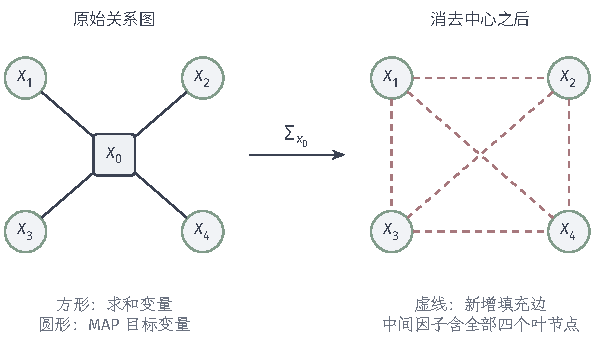
\includegraphics[width=100.651mm]{figures/09-probabilistic-graphical-models/02-inference/tikz/pgm-elimination-constrained-star/figure.pdf}
  \caption{四叶星形模型的边缘MAP消元。左图的目标是四个叶，中心$X_0$先求和；右图用虚线标出新叶间连接，记录四元输出作用域。MPE则允许先消叶，沿此顺序没有这些填充边。}
  \label{fig:pgm-elimination-constrained-star}
\end{figure}

特定参数可让式~\eqref{eq:pgm-elimination-star-map}的输出再次分解，其它算法也可利用这种结构。对仅按作用域操作的通用稠密消元，原图树宽$1$与查询受约束宽度$k$的差别却直接反映中间表增长。这解释了同一图上的边缘MAP为何可能比纯求和和MPE代价更大\scite{pgm-elimination-park2004}

\subsection{实现与适用边界}
\label{sec:pgm-elimination-implementation}

精确算法在数学上给出的是精确等式，但在计算机里用有限精度的浮点数执行时，等式可能变成带误差的近似；表很大、因子很多时这些误差还会累积。本小节讨论实现中必须处理的实际问题：表怎样按变量轴对齐、零值怎样稀疏存储、高斯矩阵怎样高效消元、连乘小数怎样避免下溢，以及什么时候精确VE根本不再可行。离散表的每一项需要以变量轴和状态编码定位，作用域信息随数值一起保存。相乘前按变量名对齐，或先转置再广播，可以使共享坐标确实表示同一状态。转置是在不改数值含义的情况下重排变量轴；广播则把缺失变量表示为长度$1$的轴，使该因子的值沿该变量的全部状态重复读取。例如将$\psi(f,h)$和$\eta(h,s)$相乘时，先统一为$(f,h,s)$轴顺序，分别用形状$(r_F,r_H,1)$和$(1,r_H,r_S)$的数组保存，再按共同的$h$索引读取并相乘，结果形状为$(r_F,r_H,r_S)$。

确定性约束产生的零项可用稀疏存储省去；消元后是否继续节省，则取决于新表非零项数。这里把函数取非零值的配置集合称为它的支持。求和会合并不同被消状态下的非零支持：若二元表仅在$(x,y)=(0,0)$和$(1,1)$处取$1$，其它项为零，则固定$x=0$和$x=1$时分别只支持一个$y$状态；求和$\tau(y)=\sum_x\psi(x,y)$后，两种$y$状态却都取$1$。原表只需保存两项非零值，输出的一元表已是稠密表。求和合并不同支持、填充扩大坐标范围，都可能令表变稠密，因此先估计峰值作用域，并在运行时记录非零项的实际增长。

高斯模型可用\term{稀疏Cholesky分解}（sparse Cholesky factorization）实现消元：将正定精度矩阵分解为三角因子，保存原非零项及新填充项。排序和符号分析先确定可能填充的位置，数值阶段再计算系数。这里的符号分析只读取非零模式，预测三角因子需要保存哪些位置；它不对概率公式作符号代数化简。例如消去一个同时连接$u,v$的标量节点时，Schur更新可能在原来为零的$(u,v)$精度块上产生新值，图中的填充边便对应这一新非零位置。相同稀疏模式可复用排序与符号结果；复用已有数值分解还要求矩阵值相同。

Schur式~\eqref{eq:pgm-elimination-schur}的逆矩阵运算可沿用前面的两次三角求解。积分常数需要的行列式也从同一分解读取：$\det(\bm{L}\bm{L}^{\top})=(\prod_j L_{j,j})^2$，且$L_{j,j}>0$，所以
\[
  \log|\bm{J}_{B,B}|=2\sum_{j=1}^{b}\log L_{j,j}.
\]
无需另求逆矩阵或先形成可能极大、极小的行列式，再取对数。

很小的权重连续相乘时，浮点数可能下溢。\term{对数域}（log domain）保存$\log\psi$，将因子乘积改为对数相加，零权重记为$-\infty$。MPE对这些和取最大值，保留同样的回溯索引。边缘查询仍需汇总所有状态，使用对数求和指数式实现这项操作：
\begin{equation}
  \log\sum_i\exp a_i
  =a_{\max}+\log\sum_i\exp(a_i-a_{\max}),
  \qquad a_{\max}=\max_i a_i.
  \label{eq:pgm-elimination-logsumexp}
\end{equation}
当$a_{\max}$有限时，减去它后至少一个指数为$1$，其余不超过$1$，避免直接对大数取指数。全体$a_i=-\infty$表示总权重零，此时直接返回$-\infty$，绕过无定义的无穷相减。若最终查询表处处零，归一化分母也为零，程序返回证据与模型不相容。

中途缩放因子也可控制数值量级。取一个与全部因子坐标无关的$s_t>0$，将$\tau_t$保存为$\widehat{\tau}_t=\tau_t/s_t$；记累计尺度$C_t=\prod_{j=1}^t s_j$，当前不变式相应为
\[
  C_t\prod_{\psi\in\widehat{\mathcal{F}}^{(t)}}\psi
  =\text{原始函数按已执行顺序聚合后的结果}.
\]
累计尺度以$\log C_t=\sum_{j=1}^t\log s_j$保存。条件分布的公共尺度最终抵消，而证据权重及最优绝对得分需恢复它。空作用域的标量因子同样影响原权重，必须明确它在累计尺度与当前因子积之间保存在哪里。本章选用的约定是：标量仍留在$\widehat{\mathcal{F}}^{(t)}$中，$C_t$只记录实际除去的$s_j$，不把同一个标量再次乘入$C_t$。例如当前另有标量$2$，把新因子$\tau$除以$3$后，恢复式为$3\times2\times(\tau/3)=2\tau$；若又把$2$乘入累计尺度而仍保留原标量，就会重复计入。

另一种等价实现是把正标量从因子集合取出，只向累计对数加入一次它的对数；这时累计尺度的记录还包括这些取出动作，不能再只记$\prod_j s_j$。两种约定不能混用。标量为零时，完整非负函数恒为零，应进入总权重零的处理分支，不能把零当作$s_t>0$的一部分取对数。

高斯核的可归一化性需要说明所用空间和测度。完整精度仅半正定、却仍在整个欧氏空间使用规范形式密度时，无二次约束方向的积分会发散。模型若限定在低维仿射子空间，应明确支持及子空间测度，在该空间上积分；伪逆和伪行列式本身不足以表达这些约定。理论正定但数值接近奇异时，检查条件数、变量尺度和分解残差以判断误差放大。对角扰动可以改善数值条件，却同时改动概率模型，应在采用时说明大小及影响。

最后说明精确VE的适用边界，以及多次查询时的复用。已知因子分解和明确查询后，可按预计中间作用域判断是否使用精确VE。离散表的高树宽或大受约束宽度可能耗尽内存；单高斯核按矩阵块维度增长，巨大块及填充也会带来高昂代价。相关信息无法全部保存时，第~\ref{chap:pgm-variational}章与第~\ref{chap:pgm-sampling}章分别通过变分和采样完成近似推断。

多次查询还涉及局部计算的复用。同一模型先问$F$再问$S$，从头消元会重复构造部分中间函数。模型与证据允许共享时，可缓存这些汇总，并在后续查询中读取或组合。判断一个缓存是否仍有效，需要记下它所依赖的原因子参数、已代入的证据值以及已经汇总的变量。相关参数或证据改变后，要重新计算受影响的缓存；若新查询需要某个已经被求和或最大化掉的变量，也不能直接从缓存恢复该变量的状态信息。沿本章原有$S,H$顺序得到的$\tau_S(h)$和$\tau_H(f)$都已消去$S$，因此不能直接拿来回答后续$S$查询。

保留两个目标坐标后，才可能供这两类查询共享。例如首次查询$F$时改为先消$H$，缓存
\[
  \eta(f,s)=\sum_h p(h\mid f)\ell_A(h,s).
\]
这张表所依赖的过热条件表、报警条件表及报警证据不变时，$F$与$S$查询分别使用
\[
  g_F(f)=p(f)\sum_s p(s)\eta(f,s),
  \qquad
  g_S(s)=p(s)\sum_f p(f)\eta(f,s).
\]
两式先给出各自的未归一化权重，再分别对全部$f$或$s$归一化得到后验。它们共享同一张没有消去$F,S$的$\eta$表，但先消$H$需要三变量桶，比原$S,H$顺序的首桶更大。单次查询的较小中间表与多次查询的复用机会由此形成实际权衡。第~\ref{chap:pgm-junction-tree}章据此组织消息与团树，减少重复工作；作用域本身很大时，其存储成本仍需承担。

\section{本章小结}
\label{sec:pgm-elimination-summary}

本章作为推断部分的开篇，把“模型给定后如何回答查询”落成一个可验证的精确算法。其主线可以用三句话概括。第一，故障后验可以直接从局部因子算出：代入报警证据，逐桶相乘并汇总非查询状态，再统一归一化；整个过程由一个不变式保证——当前乘积始终等于原函数对已消变量的聚合结果，所以局部替换与完整枚举给出相同答案。报警例的$p(F=1\mid A=1)\approx0.384111$把无故障过热、传感器失灵、误报等所有解释都汇总进分母，而MPE的$(F,H,S)=(0,1,0)$只选取单个联合最优配置，二者回答的是不同诊断任务。

第二，查询的类型决定汇总算子，也决定可用的消元顺序。边缘概率累加未知状态；MPE取最大值并保存选择、逆序恢复完整配置；边缘MAP先汇总非目标状态再选目标配置，求和与最大化的顺序一般影响答案。当目标角色限制了可用顺序后，受约束树宽可能远大于普通树宽，星形模型中“先对中心求和”会让所有叶补成团、生成多叶联合表，说明部分最优查询在结构上就可能比纯求和或MPE更贵。

第三，计算代价不由变量总数、而由消元顺序产生的中间作用域和所用函数表示共同决定。离散表按基数乘积保存状态组合，中间规模随诱导宽度指数增长；单高斯规范形式通过矩阵参数相加和Schur补解析更新，成本由矩阵块维度及填充决定。选择精确推断时，还需保证归一化合法，并控制浮点尺度与求解误差。只要中间函数能存下，VE就给出可逐步验证的精确结果；重复查询可进一步共享已算出的函数，而作用域过大时则需要额外的团树结构或明确改用近似——这正是后续章节的内容。

\paragraph{扩展阅读}
Koller与Friedman的教材从因子运算推导变量消除。书中不同顺序的例子可用于比较每桶的输入坐标、输出作用域及状态组合数，进一步理解中间函数为何比原节点总数更直接地决定成本\scite{pgm-koller2009}

\chapter{基于团树传播的精确推断}
\label{chap:pgm-junction-tree}

第~\ref{chap:pgm-elimination}章的变量消除（VE）能精确回答单个查询，但每个新查询都要从头按某个顺序消元。实际诊断往往连续提出多个相关问题：先问故障概率，随后又问过热概率，再问故障与传感器失灵的联合概率。分别运行VE会重复计算许多局部求和，例如把传感器状态汇总进过热的中间表可被多个查询复用。

团树传播把局部汇总结果组织成可在图上反复传递的\term{消息}（message）。消息以边界变量的取值为输入，记录边界一侧因子在消去内部变量后的结果。树中砍掉任意一条边都会把计算分成内部变量互不重叠的两侧，因此边界变量能明确划定一次汇总的范围。原始概率图往往带环，环上的一条边不能把节点分成互不重叠的两部分，因为两端还能绕另一条路连通。对含环图，需要先把共同处理的变量组成团，再把这些团连成一棵保留全部共享变量的树（团树），随后在树边双向传递消息，支持多次查询和局部证据更新。VE给出单次查询的局部消元步骤，团树传播则把这些步骤组织成可复用、可增量更新的结构。

以下以有限离散变量为对象，使用取有限非负值的因子。变量索引组成集合$V$，$X_i$的状态集合记为$\mathcal{X}_i$；$\bm{x}_A$表示索引集合$A\subseteq V$上一组变量取值。推断过程中模型参数固定，每个求和都遍历所标变量的全部状态，空乘积取$1$。

\section{从变量消除到消息传递}
\label{sec:pgm-junction-tree-from-elimination}

继续考虑设备诊断：二元变量$F,H,A,S$依次表示故障、过热、报警和传感器失灵，联合分布分解为
\begin{equation}
  p(f,h,a,s)=p(f)p(h\mid f)p(s)p(a\mid h,s).
  \label{eq:pgm-junction-tree-device}
\end{equation}
取$p(F=1)=0.1$、$p(S=1)=0.05$，以及$p(H=1\mid F=0)=0.1$、$p(H=1\mid F=1)=0.8$。表~\ref{tab:pgm-junction-tree-alarm-cpt}给出各状态下的报警概率；对应的未报警概率由$1$减去该值获得。这组人工设置的参数用于展示计算过程。

\begin{table}[htbp]
  \centering
  \begin{tabular}{ccc}
    \toprule
    $h$ & $s$ & $p(A=1\mid h,s)$\\
    \midrule
    $0$ & $0$ & $0.01$\\
    $1$ & $0$ & $0.90$\\
    $0$ & $1$ & $0.70$\\
    $1$ & $1$ & $0.99$\\
    \bottomrule
  \end{tabular}
  \caption{设备诊断例的报警条件概率。传感器正常时，过热使报警概率由$0.01$升至$0.90$；传感器失灵时，即使没有过热，报警概率也达到$0.70$。}
  \label{tab:pgm-junction-tree-alarm-cpt}
\end{table}

给定报警证据$A=1$，查询故障概率时先对传感器状态求和，形成关于$H$的表
\begin{equation}
  u(h)=\sum_s p(s)p(A=1\mid h,s),
  \qquad (u(0),u(1))=(0.0445,0.9045).
  \label{eq:pgm-junction-tree-boundary-likelihood}
\end{equation}
表$u(h)$已把传感器状态汇总完毕。保持模型参数和报警证据不变，故障查询和过热查询都可以读取这张表；它记录的是给定过热状态时报警侧的贡献。从另一侧消去故障变量，则得到
\begin{equation}
  v(h)=\sum_f p(f)p(h\mid f),
  \qquad (v(0),v(1))=(0.83,0.17).
  \label{eq:pgm-junction-tree-boundary-prior}
\end{equation}
表$v(h)$仅由故障先验和过热条件概率形成，它不含报警证据，因此在报警证据变化后仍可继续使用——这正体现了缓存的价值。两侧通过同一个$h$组合，得到$p(h,A=1)=u(h)v(h)$。这张关于$H$的表回答两类直接查询：对$h$求和得到报警概率$p(A=1)$，再用这个正的总和归一化，就得到$p(h\mid A=1)$。

故障变量$F$和传感器变量$S$已经分别在$v$和$u$中被求和消去，因此仅凭乘积$u(h)v(h)$，无法重新展开它们各自的状态。查询故障后验时，仍须保留$p(f)p(h\mid f)$，用$p(f)\sum_h p(h\mid f)u(h)$计算$p(f,A=1)$，然后归一化。查询$(F,S)$的联合后验时，还须在局部计算中保留$S$，或采用后文的跨团组合。这里延续了前章缓存的边界：一张表能够被哪些查询复用，取决于它保留了哪些坐标，以及形成它的参数和证据是否改变。

消息传递把中间表的变量、来源和更新方向一并记录。图~\ref{fig:pgm-junction-tree-factor-cut}给出本例的树状因子图：切断$H$与报警因子的连接后，两侧只共享$H$。给定$h$，左侧对故障求和得到$v(h)$，右侧对报警和传感器状态求和得到$u(h)$。保存整个关于$h$的函数表，使后续计算可以按所需边界状态读取；单次变量消除也可以采用这种缓存方式。

\begin{figure}[htbp]
  \centering
  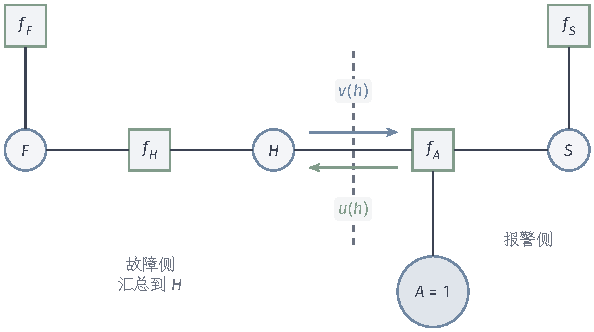
\includegraphics[width=100.651mm]{figures/09-probabilistic-graphical-models/02-inference/tikz/pgm-junction-tree-factor-cut/figure.pdf}
  \caption{设备诊断例的树状因子图。圆节点是变量，方框是因子，证据$A=1$附在报警变量处。虚线所切的两侧以$H$为共同边界，蓝色消息$v(h)$汇总故障侧，绿色消息$u(h)$汇总报警侧；箭头指示消息的发送方向。}
  \label{fig:pgm-junction-tree-factor-cut}
\end{figure}

按边界状态保存子问题结果，是动态规划在这里的具体形式。树边两侧的内部变量互不重叠，各侧的结果可以直接组合。含环图上的消息可能沿不同路径再次带回同一因子的贡献，因此需要另行处理重叠的依赖范围。

\section{树结构上的消息传递}
\label{sec:pgm-junction-tree-tree-messages}

无环因子图（因子树）上的消息规则最直接：每条边天然把图分成互不重叠的两部分，消息可由边界一侧的因子乘积定义。含环的一般图在第~\ref{sec:pgm-junction-tree-construction}节编译成团树后，再套用同一规则。在因子图中，因子$f_\alpha$对作用域$D_\alpha\subseteq V$中的变量进行局部计算，全部因子的索引组成$\mathcal{F}$。每个变量至少连接一个因子；孤立变量可接入恒为$1$的一元因子，以便用统一的消息形式处理。

证据需要先写成一个乘在变量上的因子，才能和其他因子一起参与消息计算。变量$i$处的证据记为$\ell_i(x_i)$：未观测时取$1$（不改变任何状态的权重），观测$X_i=e_i$时取指示函数$\mathbf{1}\{x_i=e_i\}$（只保留观测值、其余置零）。这样统一处理后，全部证据$\bm e$对应的权重和条件分布为
\begin{equation}
  \begin{aligned}
    q_{\bm{e}}(\bm{x})
      &=\prod_{\alpha\in\mathcal{F}}f_\alpha(\bm{x}_{D_\alpha})
        \prod_{i\in V}\ell_i(x_i),\\
    Z_{\bm{e}}&=\sum_{\bm{x}}q_{\bm{e}}(\bm{x}),\qquad
    p(\bm{x}\mid\bm{e})=\frac{q_{\bm{e}}(\bm{x})}{Z_{\bm{e}}}.
  \end{aligned}
  \label{eq:pgm-junction-tree-evidence-weight}
\end{equation}
当$Z_{\bm e}>0$时，归一化得到条件分布。观测变量仍留在图中，其后验质量集中在观测值上，因此证据变化时可以继续使用同一组变量和连接。对于无证据配分函数为$Z_0$的未归一化模型，硬证据概率等于$Z_{\bm e}/Z_0$；只有$Z_0=1$时才直接等于$Z_{\bm e}$。

\subsection{和积消息}
\label{sec:pgm-junction-tree-sum-product}

先设因子图连通且无环，即一棵树。变量$i$的相邻因子集合为$N(i)$，因子$\alpha$的相邻变量集合为$N(\alpha)=D_\alpha$。沿某条边传递的\term{和积消息}（sum-product message）汇总该边一侧的全部信息：将各分支传来的权重相乘，再对内部变量求和，只保留接收端相邻变量。变量节点和因子节点两类节点的更新式分别是
\begin{equation}
  m_{i\to\alpha}(x_i)
    =\ell_i(x_i)
      \prod_{\beta\in N(i)\setminus\{\alpha\}}
      m_{\beta\to i}(x_i),
  \label{eq:pgm-junction-tree-variable-message}
\end{equation}
\begin{equation}
  m_{\alpha\to i}(x_i)
    =\sum_{\bm{x}_{D_\alpha\setminus\{i\}}}
      f_\alpha(\bm{x}_{D_\alpha})
      \prod_{j\in D_\alpha\setminus\{i\}}
      m_{j\to\alpha}(x_j).
  \label{eq:pgm-junction-tree-factor-message}
\end{equation}
变量节点处的证据和入站消息都依赖同一个$x_i$，逐项相乘即可得到发出的表。因子节点则先固定接收变量$x_i$，把因子与其余变量的入站消息相乘，再遍历这些变量的状态求和。两类消息的输出都以$x_i$为索引。

乘积中排除接收方，是为了让消息只汇总发送侧。切断边$(i,\alpha)$，来自$\alpha$的消息汇总另一侧，乘入它就会重复计数。因子发送消息时，删除$\alpha$使其余邻接变量分属互不重叠的分支；给定这些变量的状态，各分支先独立求和。将结果与$f_\alpha$相乘，再消去接收变量以外的变量，便得到式~\eqref{eq:pgm-junction-tree-factor-message}。

把本例的四个因子写成$f_F=p(f)$、$f_H=p(h\mid f)$、$f_S=p(s)$、$f_A=p(a\mid h,s)$。图中的$F$同时连接$f_F,f_H$，$S$同时连接$f_S,f_A$，所以收集要从一元叶因子$f_F,f_S$开始。它们先发送$m_{f_F\to F}(f)=p(f)$和$m_{f_S\to S}(s)=p(s)$。故障和传感器变量都没有额外证据，其证据函数取$1$；向内部因子发送消息时，排除接收方后只剩刚收到的先验消息，因而分别得到$m_{F\to f_H}(f)=p(f)$、$m_{S\to f_A}(s)=p(s)$。报警变量$A$本身是叶节点，直接发送证据表$m_{A\to f_A}(a)=\mathbf{1}\{a=1\}$。两个相邻因子随后向$H$发送
\[
  \begin{aligned}
    m_{f_H\to H}(h)&=\sum_f p(h\mid f)p(f)=v(h),\\
    m_{f_A\to H}(h)&=\sum_{a,s}p(a\mid h,s)
       \mathbf{1}\{a=1\}p(s)=u(h).
  \end{aligned}
\]
$H$处没有额外证据，因此发往报警因子的消息为$m_{H\to f_A}=v$，发往故障因子的消息为$m_{H\to f_H}=u$。同一条边的两个方向分别携带两侧的汇总结果，各自具有不同的因子来源。树上的许多动态规划都可写成这样的局部和积运算\scite{pgm-overview-kschischang2001}

\subsection{消息调度与边缘恢复}
\label{sec:pgm-junction-tree-scheduling}

这些消息彼此有依赖关系：一条消息要等它所汇总的各分支消息先算出来。好在树上的依赖关系没有环，可以通过两轮遍历让所有消息各就各位，这就是消息调度（scheduling）。每次发送前，节点先等待除接收方之外的全部入站消息。选一个变量节点为根，从叶端向根进行\term{收集}（collect）：叶变量发送$\ell_i$，叶因子发送自身的一元函数，其余节点在分支结果到齐后继续向上发送。根收到各侧贡献后，再向叶端进行\term{分发}（distribute），把根一侧的信息逐层传下去，使每个节点最终也能收到来自父侧的贡献。

这样做的直接好处是消息数量有界且很少冗余：有$M$条边的因子树共计算$2M$条有向消息，每条边的两个方向各一次。收集按叶到根的依赖顺序完成，分发再按根到叶的顺序完成，这两轮计算就能让每条边的两个方向都有消息。根的边缘只需收集结果；查询其他位置的边缘时，分发提供它们所缺的另一侧信息。

把全部入站消息与节点处的局部输入组合，得到
\begin{equation}
  \begin{aligned}
    B_i(x_i)&=\ell_i(x_i)\prod_{\alpha\in N(i)}
       m_{\alpha\to i}(x_i),\\
    B_\alpha(\bm{x}_{D_\alpha})
      &=f_\alpha(\bm{x}_{D_\alpha})
        \prod_{j\in D_\alpha}m_{j\to\alpha}(x_j).
  \end{aligned}
  \label{eq:pgm-junction-tree-factor-beliefs}
\end{equation}
围绕$i$或$\alpha$切开树，各分支汇总其余因子，因而$B_i=\sum_{\bm{x}_{V\setminus\{i\}}}q_{\bm e}$、$B_\alpha=\sum_{\bm{x}_{V\setminus D_\alpha}}q_{\bm e}$。这两张表仍是未归一化权重；在$Z_{\bm e}>0$时，分别除以同一个$Z_{\bm e}$，才得到相应的后验边缘。若$i,j\in D_\alpha$，还可先对$B_\alpha$中其余变量求和，再保留这一步归一化，得到
\begin{equation}
  p(x_i,x_j\mid\bm e)
    =\frac{1}{Z_{\bm e}}
      \sum_{\bm{x}_{D_\alpha\setminus\{i,j\}}}
      B_\alpha(\bm{x}_{D_\alpha}).
  \label{eq:pgm-junction-tree-pair-marginal}
\end{equation}
对权重表先求和后归一化，与先将整个$B_\alpha$除以$Z_{\bm e}$再求和，得到的结果相同。成对因子的作用域正好覆盖原变量交互图的一条边；在二部因子图中，这两个变量通过同一个因子节点相连。

报警例的$H$处给出
\begin{equation}
  (B_H(0),B_H(1))=(0.036935,0.153765),
  \qquad Z_{\bm{e}}=0.19070.
  \label{eq:pgm-junction-tree-alarm-normalizer}
\end{equation}
据此得到$p(H=1\mid A=1)\approx0.806319$。向故障侧分发时，先计算$m_{f_H\to F}(f)=\sum_h p(h\mid f)u(h)=(0.1305,0.7325)$，再乘故障先验。故障状态$F=1$的权重为$0.07325$，归一化得到$p(F=1\mid A=1)=0.07325/0.19070\approx0.384111$。

这些数值保留了消息的原始尺度，在小模型上没有问题。但实际网络中，一条消息是许多小于$1$的概率连乘的结果，消息经过的因子越多，数值越小，很容易一路小到超出浮点数能表示的下限而变成$0$（下溢），即使真正的答案只是个很小、仍为正的概率。一个简单的补救是：发出消息前先整体除以一个正数把它放大，由于最终所有边缘都还要统一归一化，这种整体缩放不会改变后验。不过要计算证据概率（即未归一化的总权重$Z_{\bm e}$），就必须把这些除法逐一记录、最后补回来，否则总质量会被改变。为此，把式~\eqref{eq:pgm-junction-tree-variable-message}和式~\eqref{eq:pgm-junction-tree-factor-message}定义的原尺度消息仍记为$m$，实际保存的缩放消息记为$\widetilde m$。在每个发送方向上，另存正的累计尺度$s$，使
\[
  m_{i\to\alpha}=s_{i\to\alpha}\widetilde m_{i\to\alpha},
  \qquad
  m_{\alpha\to i}=s_{\alpha\to i}\widetilde m_{\alpha\to i}.
\]
累计尺度记录原尺度消息与存储消息之间的比例，包含它所汇总的整侧子树中的全部缩放。

具体发送时，先把已存的$\widetilde m$代入原更新式，得到尚未执行本次除法的输出$r$：
\[
  \begin{aligned}
    r_{i\to\alpha}(x_i)
      &=\ell_i(x_i)\prod_{\beta\in N(i)\setminus\{\alpha\}}
        \widetilde m_{\beta\to i}(x_i),\\
    r_{\alpha\to i}(x_i)
      &=\sum_{\bm{x}_{D_\alpha\setminus\{i\}}}
        f_\alpha(\bm{x}_{D_\alpha})
        \prod_{j\in D_\alpha\setminus\{i\}}
        \widetilde m_{j\to\alpha}(x_j).
  \end{aligned}
\]
若$r$非零，可选有限正数$c_{i\to\alpha}$或$c_{\alpha\to i}$作为本次本地除数，例如取$r$的全部表项之和，再保存$\widetilde m=r/c$。这个本地除数只记录当前发送步骤执行的除法；累计尺度还须把各入站消息已有的尺度乘回来。因此两类递推分别为
\begin{equation}
  \begin{aligned}
    s_{i\to\alpha}
      &=c_{i\to\alpha}
        \prod_{\beta\in N(i)\setminus\{\alpha\}}s_{\beta\to i},\\
    s_{\alpha\to i}
      &=c_{\alpha\to i}
        \prod_{j\in D_\alpha\setminus\{i\}}s_{j\to\alpha}.
  \end{aligned}
  \label{eq:pgm-junction-tree-factor-message-scales}
\end{equation}
这些等式来自将$m=s\widetilde m$代回原消息式：各入站尺度与边界状态无关，可以移到求和号外，再与本次除数相乘。叶端没有入站消息，对应的尺度空乘积取$1$，因此递推也包含叶端初始化。

选变量$i_0$为根，用缩放消息形成$\widetilde B_{i_0}(x_{i_0})=\ell_{i_0}(x_{i_0})\prod_{\alpha\in N(i_0)}\widetilde m_{\alpha\to i_0}(x_{i_0})$。根处的原尺度总质量为
\begin{equation}
  Z_{\bm e}
    =\left(\prod_{\alpha\in N(i_0)}s_{\alpha\to i_0}\right)
      \sum_{x_{i_0}}\widetilde B_{i_0}(x_{i_0}).
  \label{eq:pgm-junction-tree-factor-root-scale}
\end{equation}
根的各条入站消息汇总互不重叠的分支，所以只乘入根方向的累计尺度，就覆盖了全树的收集计算。若将这些累计尺度逐层展开，等价于把朝向该根的每次本地除数各乘一次；不能再把分发方向的除数也全部乘入，否则会为同一根的总质量添加不属于这次收集的尺度。报警例中，若只把$u$除以其表项之和$0.949$，而$v$保持原尺度，那么$H$处缩放表的总和为$0.19070/0.949$，恢复时只需再乘$0.949$。

如果某次$r$为全零表，就保留全零消息并取本地除数$c=1$，不能用零作除数。在精确计算中，全零消息表示发送侧在所有边界状态下都没有与证据相容的正权重配置；把它传到根后得到$Z_{\bm e}=0$，此时应报告证据不相容，不能继续形成后验。累计尺度本身也可用对数保存，以免恢复总质量之前就发生数值下溢。

\subsection{最大积消息}
\label{sec:pgm-junction-tree-max-product}

和积消息给出各状态的权重之和，对应边缘查询；MPE（见第~\ref{chap:pgm-elimination}章）要找使权重最大的一整组配置，对未知变量不再累加而取最大值。相应地，\term{最大积消息}（max-product message）以边界状态为索引，保存给定边界状态后该侧子树能够取得的最大权重，而非各状态权重之和。用$\nu$表示这套消息，只需将和积公式中的求和换成最大化，得到
\begin{equation}
  \begin{aligned}
    \nu_{i\to\alpha}(x_i)
      &=\ell_i(x_i)\prod_{\beta\in N(i)\setminus\{\alpha\}}
         \nu_{\beta\to i}(x_i),\\
    \nu_{\alpha\to i}(x_i)
      &=\max_{\bm{x}_{D_\alpha\setminus\{i\}}}
         f_\alpha(\bm{x}_{D_\alpha})
         \prod_{j\in D_\alpha\setminus\{i\}}
         \nu_{j\to\alpha}(x_j).
  \end{aligned}
  \label{eq:pgm-junction-tree-factor-max}
\end{equation}
由于分支变量互不重叠且因子非负，$\max_{\bm y,\bm z}g(\bm y)h(\bm z)=(\max_{\bm y}g)(\max_{\bm z}h)$，各侧最优值可以相乘。为了恢复最优配置，计算$\nu_{\alpha\to i}(x_i)$时，同时保存一组达到最大值的$\bm{x}_{D_\alpha\setminus\{i\}}$。这张从边界状态查找内部最优选择的表称为\term{回溯记录}（backpointer）。

将最大积入站消息全部组合，形成$\widehat{B}_i(x_i)=\ell_i(x_i)\prod_{\alpha\in N(i)}\nu_{\alpha\to i}(x_i)$。它记录固定$x_i$时全图的最大权重，称为\term{最大边缘}（max-marginal）。同一边界状态下，最大边缘取一组最优配置的权重，概率边缘则累加全部配置的权重。

收集后先在根处选择使证据与入站消息乘积最大的状态，再逐层读取回溯表：父变量状态确定后，查出相邻因子其余变量的状态，继续进入各分支。出现平局时，按固定顺序记录其中一组选择，回溯保持这组条件选择的关联。例如两个二元变量仅在$(0,0)$和$(1,1)$上权重为$1$，其余权重为零；两处最大边缘都对$0,1$平局，独立选择可能得到零权重的$(0,1)$。沿回溯记录选择，才能取得一组相容的最优解。

在设备诊断例中，以$H$为根，故障侧发送的最大权重为
\[
  \begin{aligned}
    \nu_{f_H\to H}(0)&=\max(0.9\times0.9,\;0.1\times0.2)=0.81,\\
    \nu_{f_H\to H}(1)&=\max(0.9\times0.1,\;0.1\times0.8)=0.09.
  \end{aligned}
\]
这两个$h$状态的回溯表都选$f=0$。报警侧在$h=0$时比较$0.95\times0.01$和$0.05\times0.70$，选$s=1$，权重为$0.035$；在$h=1$时比较$0.95\times0.90$和$0.05\times0.99$，选$s=0$，权重为$0.855$。根处的两个候选值为$0.02835$和$0.07695$，分别来自$0.81\times0.035$和$0.09\times0.855$，因此选$h=1$。回溯得到MPE配置$(f,h,s)=(0,1,0)$，未归一化权重为$0.07695$；报警变量保持证据值$A=1$。式~\eqref{eq:pgm-junction-tree-boundary-prior}和式~\eqref{eq:pgm-junction-tree-boundary-likelihood}中的和积表汇总全部配置，需与这套最大积表分别保存。

上面的最大积收集给出了一般因子树上的MPE算法。它有一个极为常用的特例值得单独点出：当图是一条随时间展开的链（如隐马尔可夫模型）时，最大积传播就是著名的Viterbi算法，这里用团树语言把它重新推导一遍。取长度$T\geq1$的有限状态链，记第$t$个隐状态为$Z_t$，已给定的观测为$X_t=x_t$。假设每个状态在给定前一状态后，与更早的状态条件独立；给定全部隐状态后，各时刻观测相互条件独立，而且$X_t$的条件分布只依赖$Z_t$。这里用$z_{1:t}$表示$(z_1,\ldots,z_t)$，$x_{1:t}$同理。初始分布、相邻状态的转移概率和各时刻观测概率于是组成
\[
  p(z_{1:T},x_{1:T})
    =p(z_1)p(x_1\mid z_1)
      \prod_{t=2}^{T}p(z_t\mid z_{t-1})p(x_t\mid z_t).
\]
当观测序列的概率为正时，给定观测的后验只比这个联合权重多一个与$z_{1:T}$无关的除数，所以寻找全部隐状态的联合最优配置，可以直接最大化右侧的权重。

为了向时间后端汇总，我们不必保留每一条状态前缀，只需对每个末端状态$z_t$记录到达它的最佳前缀权重。把这张表定义为
\[
  \delta_t(z_t)
    =\max_{z_{1:t-1}}p(z_{1:t},x_{1:t}).
\]
最大化遍历前$t-1$个隐状态的全部配置，固定的是当前状态$z_t$以及前$t$个观测。$t=1$时尚无更早状态，初始化为$\delta_1(z_1)=p(z_1)p(x_1\mid z_1)$。

把联合分解在最后一步拆开后，新增的因子只有$p(z_t\mid z_{t-1})$和$p(x_t\mid z_t)$。对于固定的前驱$z_{t-1}$，这两个因子都不再依赖更早的$z_{1:t-2}$，因此更早前缀只需保留其最大权重。于是对$t\geq2$有
\[
  \begin{aligned}
    \delta_t(z_t)
      &=\max_{z_{1:t-1}}
        \bigl\{p(z_{1:t-1},x_{1:t-1})
          p(z_t\mid z_{t-1})p(x_t\mid z_t)\bigr\}\\
      &=p(x_t\mid z_t)\max_{z_{t-1}}
        \left\{p(z_t\mid z_{t-1})
          \max_{z_{1:t-2}}p(z_{1:t-1},x_{1:t-1})\right\}\\
      &=p(x_t\mid z_t)
        \max_{z_{t-1}}\{\delta_{t-1}(z_{t-1})p(z_t\mid z_{t-1})\}.
  \end{aligned}
\]
这个递推中的候选只剩前一时刻的状态；每个候选此前最好的整段历史，已由$\delta_{t-1}$汇总。

计算每个$\delta_t(z_t)$时，保存一项达到括号内最大值的前驱，记为$\kappa_t(z_t)$。有限状态保证最大值能够取得，平局时按预先固定的顺序选一项。前向计算到$t=T$后，先选$z_T^\star\in\argmax_{z_T}\delta_T(z_T)$，再按$t=T,T-1,\ldots,2$依次取$z_{t-1}^\star=\kappa_t(z_t^\star)$，便得到一组相容的最优隐状态序列。这就是Viterbi动态规划：前向表保存固定边界时的最大权重，回溯表保存取得该权重的一组条件选择。若末端最大权重为零，则全部状态路径均与观测不相容，不能据此定义后验最优解释。

它求解全部隐状态的联合最优配置，第~\ref{sec:pgm-dynamic-discrete}节将用于离散时序模型。若查询仅最大化部分变量，其余变量仍须求和，应采用第~\ref{sec:pgm-elimination-map}节的边缘MAP顺序。

\section{团树的构造}
\label{sec:pgm-junction-tree-construction}

为什么朴素的“沿每条边直接发消息”在环上会失败，值得先想清楚。树上的单条边确定了两个互不重叠的内部区域，砍掉它两侧就完全分开；这个干净切分在含环图上不再成立。例如四环$1-2-3-4-1$删去边$1-2$后，$1$与$2$仍通过$1-4-3-2$相连，不能把这条边的两端当作两个互不重叠的求和分支。若仍按原来的单边消息反复汇总，同一个因子的贡献可能沿一条路发出去、又从另一条路绕回来被重复计入，得到错误结果。

解决思路不是在含环图上硬传消息，而是先改变计算单元：先扩大需要共同处理的变量集合，再确定完整的消息边界。按第~\ref{chap:pgm-elimination}章变量消除的做法，先把参与一次局部计算的因子合并，消去已经不需要保留的变量，把结果仍需共同输入的变量全部留下——这些“必须一起出现”的变量构成团。这样划分计算单元后，相邻单元的两侧可能共享多个变量；将这些变量共同保留在消息中，便可以把一片局部计算组织成树的新节点。\term{团树}（junction tree）的节点就是这样的变量团，边上的分隔集记录相邻团共享的变量。一个变量可能出现在多个团中，树上连接这些团的整条路径都须保留它，才能按同一个状态组合各处的因子。

图~\ref{fig:pgm-junction-tree-triangulation}以四环说明构造过程。消元产生的共同作用域先由填充边记录，随后用极大团容纳这些变量。将极大团连接起来，以交集为消息边界，再为原始因子选择存放位置，即可沿树边汇总两侧贡献。填充边和团节点用于组织计算，原联合分布仍由原始因子的乘积给出。

\begin{figure*}[htbp]
  \centering
  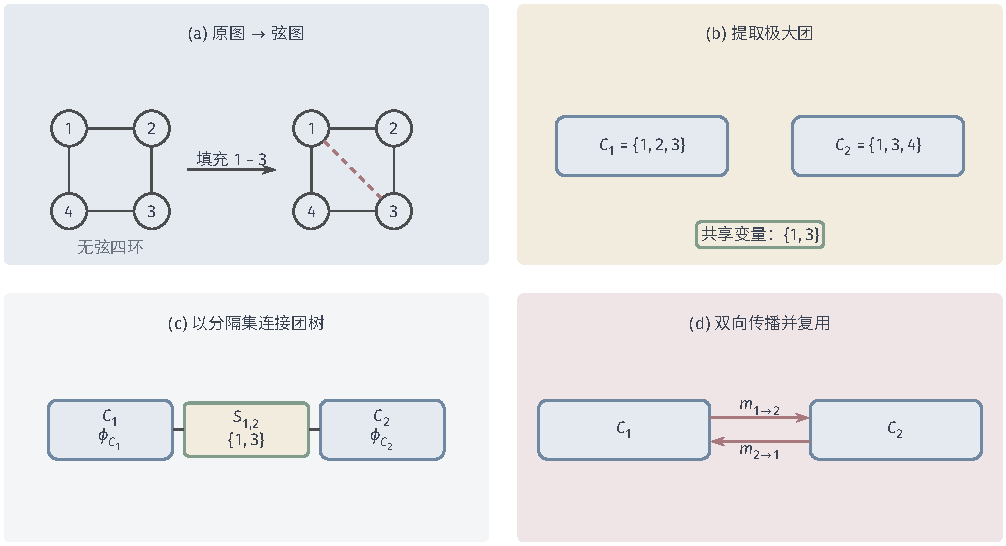
\includegraphics[width=169.000mm]{figures/09-probabilistic-graphical-models/02-inference/tikz/pgm-junction-tree-triangulation/figure.pdf}
  \caption{四环模型的团树构造与传播。添加填充边$1-3$后，两个极大团为$C_1=\{1,2,3\}$、$C_2=\{1,3,4\}$，共享变量组成分隔集$S_{1,2}=\{1,3\}$。最后一个面板在团间保存双向消息，用分隔集的状态组合两侧计算结果。}
  \label{fig:pgm-junction-tree-triangulation}
\end{figure*}

\subsection{从原图到弦图}
\label{sec:pgm-junction-tree-chordalization}

团树构造的第一步是让每个原始因子的全部变量都落在同一个团内，否则该因子无处安放。这一步对有向、无向模型略有不同。有向模型的因子$p(x_i\mid\bm{x}_{\operatorname{pa}(i)})$涉及$i$及其父节点，但父节点之间未必相连，因此先把共同子节点的父节点两两相连（道德化，见第~\ref{chap:pgm-representations}章），再去掉方向，形成承载全部因子的无向图。这里保留全部变量（与第~\ref{chap:pgm-directed}章中只按查询选取祖先子图的做法不同），因为团树要服务所有查询。在报警例中，两个报警父节点$H,S$由此相连，形成团$\{F,H\}$和$\{H,A,S\}$。

无向模型直接使用承载因子作用域的变量图；因子图则先将每个作用域中的变量两两相连。选定消元顺序后，每次把当前节点的剩余邻居全部相连，再移去该节点。将新增边保留在原变量集合上，得到\term{三角化}（triangulation）或弦化后的图；其中长度至少为$4$的环都有弦。

第~\ref{sec:pgm-elimination-complexity}节的最小度和最小填充启发式分别按剩余邻居数和缺失邻居边数选节点。填充记录消元后新因子的共同变量，每一步的求和仍完整保留被消变量的贡献。合法顺序给出相同的概率答案，但中间表和后续消息的规模可能不同。

完成填充后，所选顺序中每个节点的剩余邻居都两两相连，所以该顺序是完美消元序。有限无向图具有完美消元序，当且仅当它是弦图，因此上述填充得到的图为弦图。这里用这一结构结论保证后续能够以极大团组织局部计算；关于完美消元序、弦图和团树构造的图论依据，可参考\BookChapterRef{chap:graph-dynamic-programming}{卷一“图”部分的“图上的动态规划”章}。

填充保留消元需要的共同作用域，数值计算继续使用原因子和原参数。

对四环$1-2-3-4-1$，先消去$2$会添加$1-3$，形成极大团$\{1,2,3\}$、$\{1,3,4\}$；先消去$1$则添加$2-4$，形成$\{1,2,4\}$、$\{2,3,4\}$，如图~\ref{fig:pgm-junction-tree-triangulation}所示。两种计算都保留原分布，消息的索引却分别为$\{1,3\}$和$\{2,4\}$。这两个变量组的状态数决定了不同的消息表成本。

\subsection{极大团、分隔集与运行交集性质}
\label{sec:pgm-junction-tree-running-intersection}

团中的变量两两相连。\term{极大团}（maximal clique）指已无法加入其他节点的团；它可以小于全图节点数最多的团。记全部极大团为$\mathcal C$，以它们为节点构造树$\mathcal T=(\mathcal C,\mathcal E_{\mathcal T})$。相邻团$C,D$的交集$S_{C,D}=C\cap D$称为\term{分隔集}（separator），消息以其中变量的共同取值为索引。

极大团不能任意连成树；连接方式必须保证同一个变量的信息在传递途中不被丢失。图~\ref{fig:pgm-junction-tree-running-intersection}上排把$\{1,2\}$、$\{2,3\}$、$\{3,4\}$依次连接。含$2$的两团相邻，含$3$的两团也相邻，$1,4$各只出现在一团中。下排把$\{3,4\}$移到中间，连接含$2$的两团时需要经过一个不含$2$的团，消息无法在这条路径上保留$x_2$。

消息只能携带相邻两团交集里的变量。共享变量需要沿整条团间路径传递，若路径中途某个团删去了变量$i$，经过它的消息就无法再以$x_i$为索引，另一端的因子也无法与发送端按同一个$x_i$组合。因此团的连接还必须满足运行交集条件。

\begin{definition}[运行交集性质]
  \label{def:pgm-junction-tree-running-intersection}
  团树满足\term{运行交集性质}（running intersection property），是指对任意变量$i$，包含$i$的全部团构成连通子树。等价地，对任意两个团$C,D$，从$C$到$D$的唯一路径上的每个团都包含$C\cap D$。
\end{definition}

树中任意两团之间只有一条路径。包含$i$的团若构成连通子树，这条路径上的团都含$i$；反过来，若任意两处之间的路径都保留$i$，含$i$的团就相互连通。

\begin{figure}[htbp]
  \centering
  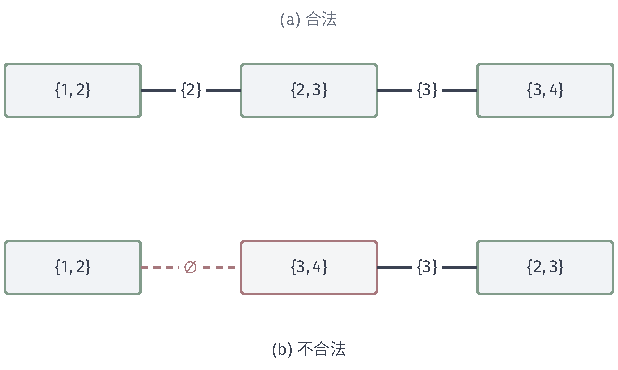
\includegraphics[width=104.652mm]{figures/09-probabilistic-graphical-models/02-inference/tikz/pgm-junction-tree-running-intersection/figure.pdf}
  \caption{运行交集性质的两种连接示例。上排每个变量出现的团都连续相连；下排连接含$2$的两团时，中间团$\{3,4\}$缺少$2$，沿该路径计算的消息会丢失共同状态$x_2$。}
  \label{fig:pgm-junction-tree-running-intersection}
\end{figure}

运行交集确定了每条消息需要保留的完整边界。删除边$(C,D)$，记$C$侧的团集合为$\mathcal C_{C\mid D}$，其中所有变量的并集为$U_{C\mid D}=\bigcup_{K\in\mathcal C_{C\mid D}}K$，则两侧的共同变量满足
\begin{equation}
  U_{C\mid D}\cap U_{D\mid C}=S_{C,D}.
  \label{eq:pgm-junction-tree-cut-intersection}
\end{equation}
$S_{C,D}$中的变量属于边的两端，所以一定出现在两侧。反之，若$i$在两侧的某个团中各出现一次，连接这两个团的路径经过$(C,D)$，运行交集迫使$C,D$都含$i$。因此两侧交集恰为$S_{C,D}$，消息可以消去其余内部变量。

给定分隔集状态，两侧便可各自求和，再相乘，这正是团树动态规划的分解方式。分配律和完整的边界保证结果精确；稠密离散表的成本仍指数依赖所选顺序的诱导宽度。实际计算需要团的状态空间足够小，能够存储并遍历这些表。

遗漏共享变量会改变求和结果，下面用一个可手算的小例说明代价。为二元链的三个团依次分配$\mathbf{1}\{x_1=x_2\}$、$\mathbf{1}\{x_2=x_3\}$、$\mathbf{1}\{x_3=x_4\}$，全局仅全$0$和全$1$的配置有非零权重，权重总和为$2$。若使用下排的错误连接（含$2$的两团被一个不含$2$的团隔开），并以$\{1,2\}$为根，$\{2,3\}$先向$\{3,4\}$发送常数$1$，后者再经空分隔集向根发送标量$2$。根的求和得到$2\times2=4$，是正确总权重的两倍：本应共享的$x_2$被分别消去，使两个局部求和各自独立、组合了彼此不相容的状态。

\subsection{团树构造与因子分配}
\label{sec:pgm-junction-tree-spanning-tree}

满足运行交集性质的团树可通过最大权生成树构造：优先连接共享变量最多的两个团，共享变量越多，消息边界越大，越不容易在中途丢失共同变量。先构造\term{团交图}（clique intersection graph）：以极大团为节点，将两团的交集大小
\[
  w(C,D)=|C\cap D|
\]
用作边权。非空交集产生正权边；对于不连通的原图，可用零权边连接不同分量，此时消息只携带空分隔集上的标量。以下把零权边也加入候选，以统一处理各连通分量。

对于非空有限弦图，把全部极大团作为节点，以交集大小为边权构成完全团图，其中保留交集为空的零权边。满足运行交集的生成树，恰好是总交集权最大的生成树。选好团间连接后，还要为团分配概率因子，计算消息和边缘。

可以用最大权Kruskal算法选边。将候选边按权重从大到小排列，平局按固定顺序处理；从空边集开始，只有两端尚未连通时才加入当前边，以保持无环。选出$|\mathcal C|-1$条边、使全部团连通后，即得到所需的最大权生成树。

对于图~\ref{fig:pgm-junction-tree-running-intersection}中的三个团，$\{1,2\}$与$\{2,3\}$共享$2$，$\{2,3\}$与$\{3,4\}$共享$3$，首尾两团交集为空。候选边权为$1,1,0$，先加入的两条正权边已经形成上排的链。余下的零权边连接已连通的两端，会形成环，因此跳过。

定理适用于已完成三角化的弦图。四环的四个边团就无法组成运行交集树，选最大权生成树也会丢失某个共享变量。三角化先决定极大团的规模，最大权选边随后保证同一变量所在的团连续相连；这一步并不优化先前的消元顺序。图模型教材进一步讨论了分解图、团树与局部计算的关系\scite{pgm-lauritzen1996}

确定树以后，将每个原始因子$f_\alpha$存入一个覆盖其全部变量的团$a(\alpha)$，即$D_\alpha\subseteq a(\alpha)$。每个因子恰好分配一次，从而得到无证据团势
\begin{equation}
  \phi_C^0(\bm{x}_C)
    =\prod_{\alpha:\,a(\alpha)=C}f_\alpha(\bm{x}_{D_\alpha}),
  \qquad
  \prod_{C\in\mathcal{C}}\phi_C^0
    =\prod_{\alpha\in\mathcal{F}}f_\alpha.
  \label{eq:pgm-junction-tree-factor-assignment}
\end{equation}
未分到因子的团取势$1$。一个因子即使被多个团覆盖，也只存放一份，否则重复乘入会改变原乘积。报警例中取$C_1=\{F,H\}$、$C_2=\{H,A,S\}$，分别存放$\phi_{C_1}^0=p(f)p(h\mid f)$、$\phi_{C_2}^0=p(s)p(a\mid h,s)$，两团通过$H$组合。

合法的分配位置、最大权树和三角化可能有多种选择，它们都保留原始因子乘积，却形成不同的局部表和缓存依赖。选择时需同时考虑消息复用和表格规模：即使团树只有很少节点，一个大团也可能需要难以容纳的状态表。

\section{团树传播}
\label{sec:pgm-junction-tree-propagation}

运行交集已经确定两团之间完整的消息边界，这一节把前面因子树上的单变量消息推广到团树上的多变量表，并给出一套两轮走完整棵树的传播算法，使所有团同时得到汇总全部证据的边缘。核心公式仍然只有乘法与求和：每个团把自己的局部势和除接收方外的所有入站消息相乘，再消去不属于分隔集的内部变量。这样可以保留因子和证据中的零表项，不必假设严格为正。

\subsection{团势与团间消息}
\label{sec:pgm-junction-tree-clique-messages}

\term{团势}（clique potential）保存分配给该团的原始因子及证据，取值非负，通常尚未归一化。它是局部计算的输入，传播完成后的边缘还需汇合全树的消息。为变量证据$\ell_i$选择一个含$i$的团$h(i)$，定义
\begin{equation}
  \phi_C(\bm{x}_C)=\phi_C^0(\bm{x}_C)
    \prod_{i:\,h(i)=C}\ell_i(x_i).
  \label{eq:pgm-junction-tree-local-evidence}
\end{equation}
每个原始因子和证据都恰好出现一次，因此$\prod_C\phi_C=q_{\bm e}$。

硬证据表示已经直接读到模型变量的准确状态。如果传感器只报告一个可能出错的结果，我们仍需保留多个潜在状态，并根据各状态产生这份报告的可能性调整其权重。设离散报告变量为$Y$，实际读数是$Y=y$，而报告的分布由模型变量$\bm X_D$决定。固定读数后，观测模型给出关于这些模型变量的似然函数
\begin{equation}
  L_y(\bm x_D)=p(Y=y\mid\bm X_D=\bm x_D).
  \label{eq:pgm-junction-tree-observation-likelihood}
\end{equation}
例如，在一组人工设置的报告参数下，$p(Y=1\mid H=0)=0.1$、$p(Y=1\mid H=1)=0.9$。收到报告$Y=1$后，两种过热状态分别乘以$0.1$和$0.9$，仍都可能保留正权重；报告本身没有直接指定过热后验等于$0.9$。后验还需结合其他因子及证据重新归一化。准确观测$X_i=e_i$可以看作报告恰等于$X_i$的特殊情形，此时似然就是$\mathbf1\{x_i=e_i\}$。

这里将上述观测似然提供的状态权重称为\term{软证据}（soft evidence），它用不同权重表达报告对候选状态的支持程度。它与直接规定一个目标边缘分布是不同的输入；若需要指定目标边缘，不能未经推导就把该分布当作似然乘入。多变量观测似然也可按相同方式吸收，但需由一个团覆盖全部作用域，并给出该似然的观测含义。加入$L_y$后，未归一化目标相应变为$q_{\bm e}L_y$，这一因子仍须恰好分配一次。一般软证据重复分配会重复乘入其权重，改变目标分布。

记团$C$的邻居集合为$N_{\mathcal T}(C)$。图~\ref{fig:pgm-junction-tree-message}展示发送$C\to D$的步骤：将$\phi_C$与除$D$之外的入站消息相乘，再对$C\setminus S_{C,D}$求和，留下分隔集上的表。反向消息按同一公式汇总$D$侧；两条消息一起提供共享变量两侧的完整贡献。

\begin{figure*}[htbp]
  \centering
  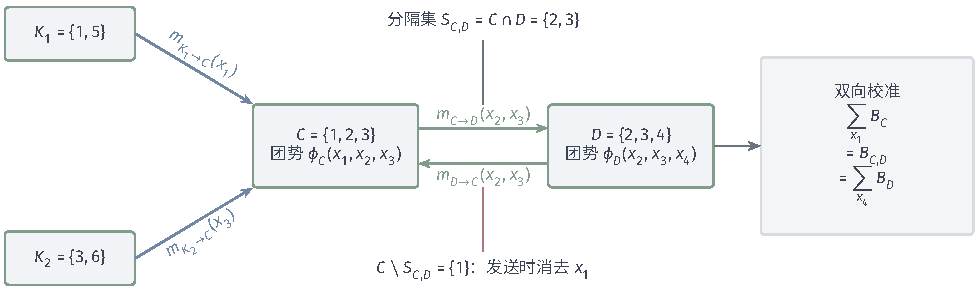
\includegraphics[width=165.650mm]{figures/09-probabilistic-graphical-models/02-inference/tikz/pgm-junction-tree-message/figure.pdf}
  \caption{团间消息与共享变量的汇总。蓝色入站消息与$\phi_C$相乘后，消去$C\setminus S_{C,D}=\{1\}$，得到以$\{2,3\}$为索引的$m_{C\to D}$；$D$侧消息留待后续组合。右侧两个方向的绿色消息共同形成$B_{C,D}$，校准后相邻团分别消去非共享变量，也得到这张分隔集表。}
  \label{fig:pgm-junction-tree-message}
\end{figure*}

对应的消息公式为
\begin{equation}
  m_{C\to D}(\bm{x}_{S_{C,D}})
    =\sum_{\bm{x}_{C\setminus S_{C,D}}}
      \phi_C(\bm{x}_C)
      \prod_{K\in N_{\mathcal{T}}(C)\setminus\{D\}}
        m_{K\to C}(\bm{x}_{S_{K,C}}).
  \label{eq:pgm-junction-tree-clique-message}
\end{equation}
计算乘积时，各函数按共同变量的状态对齐，较小作用域的函数在其余坐标上重复取值。局部势$\phi_C$保留原来的输入；新的消息另行保存，供其他方向的发送和后续查询使用。

将局部势与全部入站消息组合，并将一条边的两个方向消息组合，分别定义
\begin{equation}
  \begin{aligned}
    B_C(\bm{x}_C)
      &=\phi_C(\bm{x}_C)
        \prod_{K\in N_{\mathcal{T}}(C)}
          m_{K\to C}(\bm{x}_{S_{K,C}}),\\
    B_{C,D}(\bm{x}_{S_{C,D}})
      &=m_{C\to D}(\bm{x}_{S_{C,D}})
        m_{D\to C}(\bm{x}_{S_{C,D}}).
  \end{aligned}
  \label{eq:pgm-junction-tree-clique-separator-beliefs}
\end{equation}
传播完成后，$B_C$作为团的汇总势，包含全树对该团状态的贡献。边上的\term{分隔集势}（separator potential）$B_{C,D}$由两侧消息相乘形成，用于读取共同变量的权重。它是传播结果，原模型仍由局部团势的乘积定义。不同边即使交集相同，也各自保存双向消息和分隔集表。

把报警指示函数$\ell_A(a)=\mathbf{1}\{a=1\}$存入$C_2$，本例的局部势为
\[
  \begin{aligned}
    \phi_{C_1}(f,h)&=p(f)p(h\mid f),\\
    \phi_{C_2}(h,a,s)&=p(s)p(a\mid h,s)\ell_A(a).
  \end{aligned}
\]
每团都只有一个邻居，因此发往对方的消息直接对自身局部势求和：
\begin{equation}
  \begin{aligned}
    m_{C_1\to C_2}(h)&=\sum_f p(f)p(h\mid f)=v(h),\\
    m_{C_2\to C_1}(h)&=\sum_{a,s}p(s)p(a\mid h,s)\ell_A(a)=u(h).
  \end{aligned}
  \label{eq:pgm-junction-tree-device-clique-messages}
\end{equation}
两张表仍是前面得到的$v(h)$和$u(h)$。团树把多步局部消元合并到一次团间发送中，使用的数值运算仍是因子乘法和内部变量求和。

\subsection{收集、分发与校准}
\label{sec:pgm-junction-tree-calibration}

选团$R$为根后，先从叶团向上收集；非叶团等所有子团消息到齐，再向父团发送。根取得全部入站消息后，向各子团分发，逐层传下根侧的贡献。算法~\ref{alg:pgm-junction-tree-calibrate}按后序和先序遍历实现这两轮调度；尚未收到的消息需要等待计算，空邻居集合的乘积则取$1$。

\begin{algorithm}[团树上的和积校准]
  \label{alg:pgm-junction-tree-calibrate}
  \begin{algorithmic}[1]
    \Require 满足运行交集的团树、局部势$\{\phi_C\}$、根$R$
    \Ensure 全部双向消息、汇总势$\{B_C,B_{C,D}\}$和$Z_{\bm{e}}$
    \State 将树定根，记录每个非根团的父团
    \For{按后序遍历访问的非根团$C$}
      \State 按式~\eqref{eq:pgm-junction-tree-clique-message}发送$C$到父团的消息
    \EndFor
    \For{按先序遍历访问的团$C$}
      \For{$C$的每个子团$D$}
        \State 按式~\eqref{eq:pgm-junction-tree-clique-message}发送$C\to D$
      \EndFor
    \EndFor
    \State 按式~\eqref{eq:pgm-junction-tree-clique-separator-beliefs}形成汇总势
    \State 计算$Z_{\bm{e}}=\sum_{\bm{x}_R}B_R(\bm{x}_R)$
    \If{$Z_{\bm{e}}=0$}
      \State 报告证据与模型不相容，不输出条件概率
    \Else
      \State 令$b_C=B_C/Z_{\bm{e}}$、$b_{C,D}=B_{C,D}/Z_{\bm{e}}$
    \EndIf
  \end{algorithmic}
\end{algorithm}

双向传播后，相邻团对同一分隔集给出一致的边缘。这种重叠边缘的一致性称为\term{校准}（calibration）：各团消去非共享变量，得到同一张分隔集表。图~\ref{fig:pgm-junction-tree-message}右侧显示了这个条件；这里的校准涉及概率表之间的一致性，与分类置信度的经验校准含义不同。

对边$(C,D)$，从$C$的汇总势消去$C\setminus S_{C,D}$。入站消息$m_{D\to C}$仅依赖分隔集，能够提出求和号，于是
\begin{equation}
  \begin{aligned}
    &\sum_{\bm{x}_{C\setminus S_{C,D}}}B_C(\bm{x}_C)\\
      &\quad=m_{D\to C}
        \sum_{\bm{x}_{C\setminus S_{C,D}}}
          \phi_C\prod_{K\in N_{\mathcal{T}}(C)\setminus\{D\}}m_{K\to C}\\
      &\quad=m_{D\to C}m_{C\to D}=B_{C,D}.
  \end{aligned}
  \label{eq:pgm-junction-tree-local-calibration}
\end{equation}
从$D$侧求和也得到两条消息的乘积$B_{C,D}$，所以共享变量的汇总一致。第~\ref{sec:pgm-junction-tree-correctness}节还会把消息与原始因子的全局求和联系起来，说明这些一致的表正是输入模型的边缘。

表~\ref{tab:pgm-junction-tree-calibrated-separator}列出报警例的双向消息。固定每行的$h$，乘积给出$H=h$且发生报警的权重；最后一列的总和$0.19070$为报警概率。

\begin{table}[htbp]
  \centering
  \begin{tabular}{cccc}
    \toprule
    $h$ & $m_{C_1\to C_2}(h)$ & $m_{C_2\to C_1}(h)$ & $B_{C_1,C_2}(h)$\\
    \midrule
    $0$ & $0.83$ & $0.0445$ & $0.036935$\\
    $1$ & $0.17$ & $0.9045$ & $0.153765$\\
    \bottomrule
  \end{tabular}
  \caption{报警例的消息与分隔集权重。两条消息分别汇总故障侧和报警侧，乘积给出$p(h,A=1)$；将末列归一化便得到过热后验。}
  \label{tab:pgm-junction-tree-calibrated-separator}
\end{table}

两个团的完整汇总表如下。第一张以$f$为行、$h$为列，第二张以$h$为行、$s$为列，并只列出$a=1$切片；证据将$a=0$切片置零。
\begin{equation}
  \begin{aligned}
    \bigl[B_{C_1}(f,h)\bigr]_{f,h}
      &=\begin{pmatrix}
          0.036045&0.081405\\
          0.000890&0.072360
        \end{pmatrix},\\
    \bigl[B_{C_2}(h,1,s)\bigr]_{h,s}
      &=\begin{pmatrix}
          0.007885&0.029050\\
          0.145350&0.008415
        \end{pmatrix}.
  \end{aligned}
  \label{eq:pgm-junction-tree-device-calibrated-tables}
\end{equation}
第一张矩阵沿$f$求和，第二张沿$s$求和，都得到$(0.036935,0.153765)$，两者的总和也同为$0.19070$。这两个方向的边缘化直接显示了团表在$H$上的一致性，也核对了本例的因子分配和消息计算。

消息若分别缩放，团汇总表也会带有各自的尺度。先归一化各团表，再比较分隔集上的概率边缘，即可检查一致性。若还要恢复证据权重，则沿用式~\eqref{eq:pgm-junction-tree-factor-message-scales}中的本地除数$c$与累计尺度$s$的区别。对团间发送方向，令$m_{C\to D}=s_{C\to D}\widetilde m_{C\to D}$，其中$\widetilde m$是实际存储的表；把已缩放的入站表代入团消息式，再除以本次有限正数$c_{C\to D}$。于是
\begin{equation}
  \begin{aligned}
    s_{C\to D}
      &=c_{C\to D}\prod_{K\in N_{\mathcal T}(C)\setminus\{D\}}s_{K\to C},\\
    \widetilde B_R(\bm x_R)
      &=\phi_R(\bm x_R)\prod_{K\in N_{\mathcal T}(R)}
          \widetilde m_{K\to R}(\bm x_{S_{K,R}}),\\
    Z_{\bm e}
      &=\left(\prod_{K\in N_{\mathcal T}(R)}s_{K\to R}\right)
          \sum_{\bm x_R}\widetilde B_R(\bm x_R).
  \end{aligned}
  \label{eq:pgm-junction-tree-clique-message-scales}
\end{equation}
根团各入站消息的源侧恰好覆盖其余团，且局部因子各计一次，因此恢复总质量只需要这些入根累计尺度。零消息仍取本地除数$1$并保留全零表；此时可以判断证据不相容，但不能用零总和归一化。通过局部表示吸收证据并沿连接传播，是经典精确图模型推断的方法\scite{pgm-overview-lauritzen1988}

\subsection{查询与证据更新}
\label{sec:pgm-junction-tree-queries-updates}

校准之后，多数查询只需在现成的团表上做少量求和，不必重新传播。若查询由单个团覆盖，可直接对团内其余变量边缘化；跨团查询则要处理相邻团汇总表的重复计数，两张表相乘会重复计入分隔集上的权重，必须除掉。

若查询集合$Q$由某个团$C$覆盖（$Q\subseteq C$），由于$B_C$已经汇总了全图证据，对团内其余变量求和并归一化就直接得到
\begin{equation}
  p(\bm{x}_Q\mid\bm{e})
    =\sum_{\bm{x}_{C\setminus Q}}b_C(\bm{x}_C).
  \label{eq:pgm-junction-tree-covered-query}
\end{equation}
这一步复用现有消息，只计算团内的边缘化及输出表。报警例的$F,H$在$C_1$中，$H,S$在$C_2$中；相应地消去$H$，得到$p(F=1\mid A=1)\approx0.384111$和$p(S=1\mid A=1)\approx0.196460$。

查询$\{F,S\}$需要结合两个团。两团的汇总势各自包含全图贡献，直接相乘会再次计入共同的$H$权重。为确定重复的是哪一项，我们把两张汇总表按其来源展开。在$a=1$切片上，
\[
  \begin{aligned}
    B_{C_1}(f,h)&=\phi_{C_1}(f,h)u(h),\\
    B_{C_2}(h,1,s)&=\phi_{C_2}(h,1,s)v(h),\\
    B_{C_1,C_2}(h)&=u(h)v(h).
  \end{aligned}
\]
前两式各含一侧的局部势和另一侧的汇总，因而相乘时多出$u(h)v(h)$。在该乘积为正的$h$状态上，逐项消去这份重复贡献，得到
\[
  \begin{aligned}
    \frac{B_{C_1}(f,h)B_{C_2}(h,1,s)}{B_{C_1,C_2}(h)}
      &=\frac{\phi_{C_1}(f,h)u(h)\phi_{C_2}(h,1,s)v(h)}{u(h)v(h)}\\
      &=\phi_{C_1}(f,h)\phi_{C_2}(h,1,s)\\
      &=p(f)p(h\mid f)p(s)p(A=1\mid h,s).
  \end{aligned}
\]
右侧恰好是保留$f,h,s$和报警证据的原始联合权重，没有额外改变两个$h$状态的相对贡献。将这份重复权重除去，再消去$H$，本例得到
\begin{equation}
  p(f,s\mid A=1)
    =\frac{1}{Z_{\bm{e}}}
      \sum_h
       \frac{B_{C_1}(f,h)B_{C_2}(h,1,s)}
            {B_{C_1,C_2}(h)}.
  \label{eq:pgm-junction-tree-cross-clique-device}
\end{equation}
本例两种$h$状态的分母都为正。固定$(f,s)=(0,0)$，归一化前的两个$h$项为
\[
  \begin{aligned}
    &\frac{0.036045\times0.007885}{0.036935}
     +\frac{0.081405\times0.145350}{0.153765}\\
    &=0.007695+0.076950=0.084645.
  \end{aligned}
\]
除以分隔集势以后，每个$h$状态的共同贡献只保留一份。表~\ref{tab:pgm-junction-tree-cross-query}给出四组$(f,s)$的结果，与直接消去$H$的联合表一致。

\begin{table}[htbp]
  \centering
  \begin{tabular}{cccc}
    \toprule
    $f$ & $s$ & $p(f,s,A=1)$ & $p(f,s\mid A=1)$\\
    \midrule
    $0$ & $0$ & $0.084645$ & $0.443865$\\
    $0$ & $1$ & $0.032805$ & $0.172024$\\
    $1$ & $0$ & $0.068590$ & $0.359675$\\
    $1$ & $1$ & $0.004660$ & $0.024436$\\
    \bottomrule
  \end{tabular}
  \caption{跨团查询$(F,S)$的联合权重与后验。先按分隔集$H$组合两团的汇总表，再消去$H$；末列保留六位小数，显示两个查询变量在报警证据下的联合分布。}
  \label{tab:pgm-junction-tree-cross-query}
\end{table}

重复的分隔集权重随$h$变化，因此会改变相对概率。直接把两团表相乘再求和，将得到
\[
  \widetilde{q}(f,s)=\sum_h B_{C_1}(f,h)B_{C_2}(h,1,s).
\]
对这个$\widetilde q$归一化后，故障概率约为$0.446232$，偏离正确的$0.384111$。多乘的$B_{C_1,C_2}(h)$改变了两种$h$状态的相对权重，整体归一化只能消去常数尺度。

一般跨团查询可以保留连接查询变量的团子树。先为每个查询变量选一个包含它的团，将连接这些团的子树节点记为$\mathcal H\subseteq\mathcal C$，所有相关变量的并集记为$W=\bigcup_{C\in\mathcal H}C$。把树外分支的既有消息吸收到子树局部势，计算
\begin{equation}
  \begin{aligned}
    \widetilde{\phi}_C
      &=\phi_C
        \prod_{D\in N_{\mathcal{T}}(C)\setminus\mathcal{H}}m_{D\to C},\\
    g_Q(\bm{x}_Q)
      &=\sum_{\bm{x}_{W\setminus Q}}
         \prod_{C\in\mathcal{H}}\widetilde{\phi}_C(\bm{x}_C),\\
    p(\bm{x}_Q\mid\bm{e})&=g_Q(\bm{x}_Q)/Z_{\bm{e}}.
  \end{aligned}
  \label{eq:pgm-junction-tree-subtree-query}
\end{equation}
运行交集使每个外部分支只经自己的分隔集连接这棵子树，入站消息已完成对$V\setminus W$的求和。随后在子树内部消元，即可得到$g_Q$；可以逐步计算中间表，避免直接展开整个$W$联合表。这一表达只用乘法和求和，也适用于零表项。

若只保存校准后的团边缘与分隔集边缘，则可在分隔集概率为正的状态上重构
\begin{equation}
  p(\bm{x}_W\mid\bm{e})
    =\frac{\prod_{C\in\mathcal{H}}b_C(\bm{x}_C)}
           {\prod_{(C,D)\in\mathcal{E}_{\mathcal{H}}}
                b_{C,D}(\bm{x}_{S_{C,D}})},
  \label{eq:pgm-junction-tree-calibrated-factorization}
\end{equation}
其中$\mathcal E_{\mathcal H}$为子树的内部边集，再消去$W\setminus Q$便得到查询结果。代入式~\eqref{eq:pgm-junction-tree-clique-separator-beliefs}，每条内部边的两个方向消息各约去一次，剩下$\prod_C\widetilde\phi_C$。树的节点数比边数多一，归一化因子也相应剩下$1/Z_{\bm e}$，得到与式~\eqref{eq:pgm-junction-tree-subtree-query}相同的结果。

分隔集概率为零时，所有与该状态一致的完整配置概率也为零。可直接用无除法的式~\eqref{eq:pgm-junction-tree-subtree-query}计算；也可对子树定根，仅在正概率的父分隔集状态上用团边缘与分隔集边缘的比值形成条件表。下面把后一种补零过程写清，以免把某个零状态误解为整条分支都应删除。

取子树$\mathcal H$的根团为$R$。每个非根团$C$的父团记为$\operatorname{pa}_{\mathcal H}(C)$，相应父分隔集为$S_C=C\cap\operatorname{pa}_{\mathcal H}(C)$。进入$C$时，$S_C$中的变量已经由此前的团赋值；运行交集保证$C$与已处理部分的全部重叠恰好包含在$S_C$中，新增的变量是$C\setminus S_C$。定义表
\begin{equation}
  \kappa_C(\bm x_{C\setminus S_C}\mid\bm x_{S_C})
  =\begin{cases}
    \displaystyle\frac{b_C(\bm x_C)}
      {b_{C,\operatorname{pa}_{\mathcal H}(C)}(\bm x_{S_C})},
      &b_{C,\operatorname{pa}_{\mathcal H}(C)}(\bm x_{S_C})>0,\\[6pt]
    0,&b_{C,\operatorname{pa}_{\mathcal H}(C)}(\bm x_{S_C})=0.
  \end{cases}
  \label{eq:pgm-junction-tree-zero-separator-conditional}
\end{equation}
对正概率的父分隔集状态，校准保证分子对$C\setminus S_C$求和等于分母，所以$\kappa_C$在这些状态上是归一化的条件表。父分隔集概率为零时，与之相容的每个$b_C$表项也为零；这里将这些父状态对应的表项整体赋零，仅作为联合重构的约定，不把它们称为已定义的条件概率。于是从根边缘开始，依次加入各团的新变量，得到
\begin{equation}
  p(\bm x_W\mid\bm e)
    =b_R(\bm x_R)
      \prod_{C\in\mathcal H\setminus\{R\}}
        \kappa_C(\bm x_{C\setminus S_C}\mid\bm x_{S_C}).
  \label{eq:pgm-junction-tree-rooted-reconstruction}
\end{equation}
在所有父分隔集概率都为正的配置上，它就是前面的团边缘除分隔集边缘公式。若某个父状态概率为零，该状态对应的联合质量原本就是零，补零只作用于这些配置，不会消去同一分支上其他正概率父状态的贡献。这样可为式~\eqref{eq:pgm-junction-tree-calibrated-factorization}在零概率状态上补零。查询少量边缘时可继续局部消元，而大规模联合表还需要支付写出全部表项的成本。

查询一组MPE时，另行计算最大积消息$\nu_{C\to D}$。消息内部使用最大化，并为每个分隔集状态保存内部最优选择
\begin{equation}
  \rho_{C\to D}(\bm{x}_{S_{C,D}})
    \in\argmax_{\bm{x}_{C\setminus S_{C,D}}}
       \left\{\phi_C
          \prod_{K\in N_{\mathcal{T}}(C)\setminus\{D\}}\nu_{K\to C}\right\}.
  \label{eq:pgm-junction-tree-clique-backpointer}
\end{equation}
先在根团选择最优配置，再根据已确定的分隔集状态向外回溯。运行交集把已赋值部分与新分支的全部重叠保留在分隔集中，因而各步能共享同一组变量值。求一组MPE只需收集和回溯；读取所有团的最大边缘时，再计算双向最大积消息，并用最大化检查重叠一致性。这套汇总表存储最优权重，需与概率边缘分别使用。和积传播的结果提供求和信息，MPE仍需完成相应的最大化与配置恢复运算。

团树的另一个实用优势在证据改变时体现：很多消息可以原样复用，只需重算真正受影响的方向。判断依据很直接——一条消息只汇总它源侧各团的局部势。设局部势改变的团组成$\mathcal D$。消息$m_{C\to D}$只汇总源侧$\mathcal C_{C\mid D}$的局部势，因此
\begin{equation}
  \mathcal{C}_{C\mid D}\cap\mathcal{D}=\varnothing
  \quad\Longrightarrow\quad
  m_{C\to D}\text{可原样复用}.
  \label{eq:pgm-junction-tree-update-dependency}
\end{equation}
若源侧包含变化团，该消息需标记为可能失效。个别数值变化可能恰好抵消，使消息仍相同，但源侧依赖关系只保证式~\eqref{eq:pgm-junction-tree-update-dependency}中的复用条件。

只有$C_0$变化时，朝向它的消息汇总其他侧的局部势，可原样保留；以$C_0$为根重新分发，重算每条边向外的一个方向即可。图~\ref{fig:pgm-junction-tree-evidence-update}给出这组方向。若只查询$C_q$覆盖的变量，更新$C_0$到$C_q$的路径就已足够，其他分支向路径发来的消息仍有效。路径以外尚未重算的团表继续保留失效标记，因为一个局部输入变化也可能影响全树后验。

路径上的消息完成更新后，还要形成与新证据对应的查询团表。记更新后的局部势和有效消息为$\phi'_{C_q}$、$m'_{D\to C_q}$，其中未受影响的输入沿用旧值。先计算
\begin{equation}
  \begin{aligned}
    B'_{C_q}(\bm x_{C_q})
      &=\phi'_{C_q}(\bm x_{C_q})
        \prod_{D\in N_{\mathcal T}(C_q)}m'_{D\to C_q}(\bm x_{S_{D,C_q}}),\\
    Z'_{\bm e}&=\sum_{\bm x_{C_q}}B'_{C_q}(\bm x_{C_q}).
  \end{aligned}
  \label{eq:pgm-junction-tree-updated-query-normalizer}
\end{equation}
这里采用原尺度消息；若消息经过缩放，按前述累计尺度恢复总质量。$Z'_{\bm e}>0$时，对$B'_{C_q}$消去非查询变量，再除以这个新的常数，才得到新证据下的后验。旧的团汇总表和旧的$Z_{\bm e}$都不能直接复用；$Z'_{\bm e}=0$时报告新证据与模型不相容，不输出条件概率。

多个团同时改变时，分别按源侧是否包含变化团判断，某条边的两个方向都可能失效。

\begin{figure}[htbp]
  \centering
  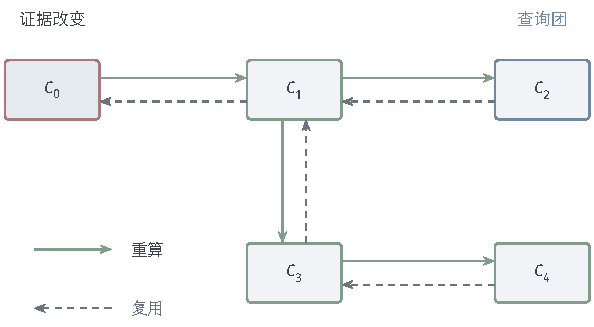
\includegraphics[width=100.651mm]{figures/09-probabilistic-graphical-models/02-inference/tikz/pgm-junction-tree-evidence-update/figure.pdf}
  \caption{单个团势变化后的消息更新。$C_0$改变后，实线方向重新汇总含$C_0$一侧的贡献，反向虚线消息继续复用。查询$C_2$只需更新$C_0-C_1-C_2$路径；其他团表需在其入站消息也更新后才能用于新证据。团的具体变量集合仍须满足运行交集性质。}
  \label{fig:pgm-junction-tree-evidence-update}
\end{figure}

报警例中新观测到$S=0$，变化仅发生在$C_2$。保留$m_{C_1\to C_2}=(0.83,0.17)$，重算$m_{C_2\to C_1}=(0.0095,0.855)$，得到$Z_{\bm e}=p(A=1,S=0)=0.153235$，故障后验为$0.068590/0.153235\approx0.447613$。若将原先单独的报警证据改为$A=0$，反向消息变为$(0.9555,0.0955)$，证据概率为$0.80930$，故障后验为$0.02675/0.80930\approx0.033053$。这两次修改都保留故障侧的先验汇总。

撤回硬证据需要从原始输入恢复团势。旧指示函数已把部分表项置零，对其相除无法找回这些值，因此保留$\phi_C^0$及每条当前证据，按式~\eqref{eq:pgm-junction-tree-local-evidence}重新形成受影响的局部势。随后按源侧依赖重算消息及其缩放常数。若先前还按证据删去变量或裁剪连接，撤回时需一并恢复这些结构。

在原有作用域内修改因子数值，或加入被现有团覆盖的观测似然，都可以沿当前团树更新。新作用域超出现有团时，则要重新分配因子、扩大团或重新三角化，以容纳新增的共同变量。更新后若$Z_{\bm e}=0$，包括硬证据互相矛盾的情形，传播得到零总权重，条件后验没有定义。缓存更新因而同时依赖作用域覆盖、消息来源和正的归一化常数。

\section{算法分析}
\label{sec:pgm-junction-tree-analysis}

\subsection{正确性与校准}
\label{sec:pgm-junction-tree-correctness}

前面通过校准现象（相邻团对分隔集给出同一张表）观察到传播结果是自洽的，但“自洽”还不等于“正确”——一组彼此一致的表未必对应原来的概率模型。这一节要证明更强的结论：每条消息恰好等于源侧全部因子对内部变量求和的结果，因而团表和分隔集表正是原始模型的真实（未归一化）边缘。同时也界定连续情形下需要单独核查的条件。校准给出重叠表的一致性，消息的子树含义则把这些表与原始模型联系起来。下面将一条消息写成源侧全部局部势的求和，进而证明团表确实是所需边缘；同一含义也确定跨团查询的边界和证据更新的依赖范围。

\begin{theorem}[子树消息与团边缘]
  \label{thm:pgm-junction-tree-correctness}
  设$V$为有限变量索引集，每个$X_i$的状态空间有限非空；$\mathcal{T}=(\mathcal{C},\mathcal{E}_{\mathcal T})$是以$V$的子集为团节点、满足$\bigcup_{C\in\mathcal C}C=V$和运行交集性质的有限树。有限个取有限非负值的因子与证据因子恰好各分配给一个覆盖其作用域的团，所得团势为$\phi_C$，并记未归一化目标$q_{\bm e}(\bm{x})=\prod_{C\in\mathcal C}\phi_C(\bm{x}_C)$。对边$(C,D)$，令$S_{C,D}=C\cap D$；删除该边后，记$C$侧的团集合为$\mathcal{C}_{C\mid D}$，并令$U_{C\mid D}=\bigcup_{K\in\mathcal{C}_{C\mid D}}K$。若按式~\eqref{eq:pgm-junction-tree-clique-message}完成全部未缩放和积消息，则对每条有向边$C\to D$，
  \begin{equation}
    m_{C\to D}(\bm{x}_{S_{C,D}})
      =\sum_{\bm{x}_{U_{C\mid D}\setminus S_{C,D}}}
         \prod_{K\in\mathcal{C}_{C\mid D}}\phi_K(\bm{x}_K).
    \label{eq:pgm-junction-tree-subtree-invariant}
  \end{equation}
  完整传播后，定义
  \[
    \begin{aligned}
      B_C(\bm{x}_C)&\mathrel{:=}
        \phi_C(\bm{x}_C)
        \prod_{K\in N_{\mathcal{T}}(C)}
          m_{K\to C}(\bm{x}_{S_{K,C}}),\\
      B_{C,D}(\bm{x}_{S_{C,D}})&\mathrel{:=}
        m_{C\to D}(\bm{x}_{S_{C,D}})
        m_{D\to C}(\bm{x}_{S_{C,D}}),\\
      Z_{\bm e}&\mathrel{:=}
        \sum_{\bm{x}_V}q_{\bm e}(\bm{x}).
    \end{aligned}
  \]
  则对任意团$C$及边$(C,D)$，
  \begin{equation}
    \begin{aligned}
      B_C(\bm{x}_C)
        &=\sum_{\bm{x}_{V\setminus C}}q_{\bm{e}}(\bm{x}),\\
      B_{C,D}(\bm{x}_{S_{C,D}})
        &=\sum_{\bm{x}_{V\setminus S_{C,D}}}q_{\bm{e}}(\bm{x}).
    \end{aligned}
    \label{eq:pgm-junction-tree-true-marginals}
  \end{equation}
  若$Z_{\bm e}>0$，则$B_C/Z_{\bm e}$与$B_{C,D}/Z_{\bm e}$分别为相应的后验团边缘和后验分隔集边缘。
\end{theorem}

\begin{proof}
  按源侧$\mathcal C_{C\mid D}$的团数归纳。若只有叶团$C$，这一侧的全部输入就是$\phi_C$，消去$C\setminus S_{C,D}$即得到式~\eqref{eq:pgm-junction-tree-subtree-invariant}。

  对源侧含多个团的情况，删除$C$后，除$D$侧外的每个邻团$K$各形成一个分支，内部变量为$R_K=U_{K\mid C}\setminus S_{K,C}$。若变量同时出现在该分支和$C$，连接两处的路径经过$K$，运行交集使它属于$S_{K,C}$，所以$R_K$与$C$不交。若两个分支的内部集合共享某变量，连接这两处的路径经过$C$，运行交集又要求它属于$C$，与内部变量定义矛盾。因此各$R_K$彼此也不交。

  要消去的$U_{C\mid D}\setminus S_{C,D}$由$C\setminus S_{C,D}$和各分支内部$R_K$组成。固定$\bm{x}_C$后，这些分支可以分别求和，归纳假设将每一项识别为$m_{K\to C}$。再用有限求和的分配律，可得
  \[
    \begin{aligned}
      &\sum_{\bm{x}_{U_{C\mid D}\setminus S_{C,D}}}
         \prod_{L\in\mathcal{C}_{C\mid D}}\phi_L\\
      &\quad=\sum_{\bm{x}_{C\setminus S_{C,D}}}\phi_C
         \prod_{K\in N_{\mathcal{T}}(C)\setminus\{D\}}
          \left[
            \sum_{\bm{x}_{R_K}}
              \prod_{L\in\mathcal{C}_{K\mid C}}\phi_L
          \right]\\
      &\quad=\sum_{\bm{x}_{C\setminus S_{C,D}}}\phi_C
         \prod_{K\in N_{\mathcal{T}}(C)\setminus\{D\}}m_{K\to C}.
    \end{aligned}
  \]
  该式最后一行就是$C\to D$的更新公式，因此归纳式对整个源侧成立。

  固定任意团$C$，用同样的分解纳入全部邻接分支。它们的内部变量互不重叠，与$C$共同覆盖$V$，局部势又各出现一次，乘积为$q_{\bm e}$。先对各分支内部求和，就留下$\phi_C\prod_Km_{K\to C}=B_C$，得到团边缘等式。再对$C\setminus S_{C,D}$求和，式~\eqref{eq:pgm-junction-tree-local-calibration}给出分隔集边缘$B_{C,D}$。将任一表对其全部状态求和，均得$Z_{\bm e}$；若它为正，归一化即得后验边缘。
\end{proof}

这项证明逐一使用了两个结构条件：运行交集把全部共享变量留在分隔集中，使各分支的内部变量互不重叠；唯一因子分配使局部势的乘积恰为输入模型。于是分配律可以把全局求和拆成消息。仅从一组归一化且相邻一致的表出发，可以重构满足它们的分布，但要确认它就是原模型，还需要上述与原始因子乘积的联系。

在相同的子树分解中，将求和换成最大化，非负因子的分配律给出最大积消息的最优值。给定分隔集状态，回溯表保存的内部选择取得这条消息的值；每次展开时，已有赋值与新分支仅在分隔集中重叠。沿树代入这些选择，最终配置的联合权重就达到根的最大值。根最大值为零时，全部配置的权重都为零，条件分布及其条件MPE均没有定义。

因子和消息可以含零表项，和积与最大积证明都仍成立；正表项主要便于采用比值形式重构。上面的定理以有限离散状态为前提。将和积消息推广到连续变量时，需要恢复第~\ref{sec:pgm-elimination-correctness}节中两类不同的积分条件：每步消息能否成为有限函数，以及完整目标能否归一化。这两项条件分别服务于局部运算和概率解释。

具体地，设每个变量空间带有$\sigma$有限基准测度$\mu_i$。对指标集合$A$，变量组的状态空间记为$\mathcal X_A=\prod_{i\in A}\mathcal X_i$，乘积测度记为$\mu_A=\bigotimes_{i\in A}\mu_i$；空指标集采用单点空间及其单位测度。局部势继续取有限非负值，并要求可测；证据已通过指定的观测似然或条件密度吸收到局部势中。若固定并移除了连续观测坐标，以下的$V$只表示剩余的积分坐标，团及分隔集也相应限制到这些坐标。对每条有向边$C\to D$，用积分形成消息时，要求
\begin{equation}
  \int_{\mathcal X_{C\setminus S_{C,D}}}
    \phi_C(\bm{x}_C)
    \prod_{K\in N_{\mathcal T}(C)\setminus\{D\}}
      m_{K\to C}(\bm{x}_{S_{K,C}})
    \,\mathrm{d}\mu_{C\setminus S_{C,D}}
    (\bm{x}_{C\setminus S_{C,D}})<\infty
  \label{eq:pgm-junction-tree-local-integrability}
\end{equation}
对$\mu_{S_{C,D}}$几乎处处的边界状态成立。也就是说，允许局部积分只在一个边界零测集上发散；在这个集合上可统一把消息指定为$0$，从而选取与积分几乎处处相同的有限非负可测版本。后续计算使用这些有限版本，才能继续按普通实值函数作乘法。

Tonelli定理允许交换非负可测函数的积分次序，即使某个积分为无穷也仍可成立；它本身不保证局部消息有限。在上述局部有限性条件下，子树证明中的求和可改为积分，消息等式按分隔集测度几乎处处成立，团边缘等式按对应团坐标的测度几乎处处成立。采用有限版本时改变的只是零测集；$\sigma$有限的乘积测度保证这些例外集提升到更多坐标后仍为零测集，Tonelli定理又保证继续积分时只影响几乎处处的等式。若还要把团汇总函数解释为后验密度，则另须检查完整目标的总质量
\begin{equation}
  0<Z_{\bm e}
    =\int_{\mathcal X_V}q_{\bm e}(\bm{x}_V)
       \,\mathrm{d}\mu_V(\bm{x}_V)<\infty.
  \label{eq:pgm-junction-tree-continuous-normalizer}
\end{equation}
这时$B_C/Z_{\bm e}$和$B_{C,D}/Z_{\bm e}$分别给出后验团密度和后验分隔集密度的版本，其等式仍是几乎处处的密度等式。

完整目标可积并不能替代每条源侧消息的有限性。例如，取三个实值变量$X,Y,Z$，将其取值记为$x,y,z$，并采用Lebesgue基准测度。以$\{X\}$连接两个团$C=\{X,Y\}$、$D=\{X,Z\}$，并设置
\[
  \phi_C(x,y)=
    \begin{cases}
      \exp(-y^2),&x\le0,\\
      1,&x>0,
    \end{cases}
  \qquad
  \phi_D(x,z)=\mathbf1\{x\le0\}\exp(-x^2-z^2).
\]
完整乘积为$\mathbf1\{x\le0\}\exp(-x^2-y^2-z^2)$，总质量为$\pi^{3/2}/2$，有限且为正。但是$C\to D$对$y$的积分在$x>0$时为无穷，反向消息在同一区域为零；该区域在分隔集测度下并非零测集。直接沿用有限表的普通乘法，就会遇到$0\times\infty$，无法把这条发散消息当作有限消息传递。这个例子说明，全局归一化条件与局部有限性条件需要分别核查。

即使局部积分存在，也还需能够精确计算它，才能保持本章精确传播的结论，实际表达取决于函数形式。高斯势的局部乘积若对被积分向量$\bm y$具有二次指数形式，则沿用第~\ref{sec:pgm-elimination-gaussian}节的条件：$\bm y$对应的二次型矩阵块必须正定，才能完成有限的高斯积分，再以Schur补形成输出。这个被积分块的条件与完整模型总质量的检查承担不同职责。

连续观测还要明确采用哪个条件密度版本或观测模型。用观测似然$g(\bm e\mid\bm{x})$时，先固定已给定的观测值$\bm e$，将这个关于未知状态的非负函数乘入目标。若从联合密度取观测切片来形成条件密度，密度比的解释要求观测边缘密度正且有限，并在相应的几乎处处口径下成立。通常连续基准测度中的单点指示函数只有零积分，无法直接产生离散硬证据那样的概率质量；不能把保留离散观测节点的写法直接照搬到这种连续观测中。

\subsection{与变量消除的关系}
\label{sec:pgm-junction-tree-ve-relation}

团树与第~\ref{chap:pgm-elimination}章的变量消除是同一套局部计算的两种组织方式：团树把VE每一步产生的中间因子（消息）连同依赖关系保存下来并连成树。下面的对应关系说明两种算法为何给出相同结果，以及各自适合的使用场景。

三角化已经记录了变量消除产生的共同作用域。为了把逐步消元的记录连成树，取完整顺序$\pi=(v_1,\ldots,v_n)$，其中$n=|V|$，并令$N_i^+$表示消去$v_i$时尚未消去的邻居。消去$v_i$时，相关因子的乘积作用域包含在$\{v_i\}\cup N_i^+$中，输出以$N_i^+$为边界。我们把这个容纳当前变量和全部边界变量的集合记为消元袋
\begin{equation}
  K_i=\{v_i\}\cup N_i^+.
  \label{eq:pgm-junction-tree-elimination-bag}
\end{equation}
袋在这里表示一次局部计算所需的变量集合；不同袋可以相互包含，因而它们还不全是极大团。若$V=\varnothing$，用一个空袋保存标量乘积即可；以下讨论$n\ge1$的情形。

当$N_i^+\neq\varnothing$时，从中选取消元顺序最靠前的后继变量$v_{p(i)}$，即
\[
  p(i)=\min\{j>i:v_j\in N_i^+\},
\]
把$K_{p(i)}$作为$K_i$的父袋，并连接$K_i-K_{p(i)}$。消去$v_i$时，填充已把$N_i^+$连成团。除$v_{p(i)}$本身以外，$N_i^+$中的变量都晚于$v_{p(i)}$消去，且与它相邻，因此都属于$N_{p(i)}^+$。于是$N_i^+\subseteq K_{p(i)}$，生成的新因子能够完整地送入父袋，其边界没有丢失。保存每个袋及其生成的新因子，就记录了这些局部计算之间的消息依赖。

沿父边移动时，袋的序号严格增加，所以不会出现环；$N_i^+=\varnothing$的袋作为根。每个输入连通分量得到一棵这样的树。输入不连通时，先得到森林，再以空分隔集连接不同分量的根，便可用同一棵树组织计算；空分隔集上的消息是一个标量，汇总相应分量的总权重。

这些父边也保证运行交集性质。若变量$v_j$属于较早的袋$K_i$，则$v_j\in N_i^+$，父袋仍包含$v_j$，且父袋序号不超过$j$。反复沿父边上行，序号不断增大，最终到达$K_j$，途中每个袋都保留$v_j$。因此，所有含$v_j$的袋都通过含它的路径连接到$K_j$，构成连通子树。原始因子可分配到消去其最早变量时的袋中：它的其他作用域变量在这一步都尚未消去，而且与当前变量相邻，所以整个作用域被该袋覆盖。标量因子可分配到任一根；每个因子仍须恰好分配一次。这样，袋树既保留了共享变量，也保留了原始因子乘积。

袋树中的包含关系还可以减少节点数。若一个非极大袋$K$包含在某个较大的极大袋$L$中，运行交集要求从$K$到$L$的路径上每个袋都包含$K$的全部变量，所以紧邻$K$的下一个袋已经包含$K$。可以把这条边收缩：保留相邻的较大袋，将$K$的局部输入归并到该袋，并把$K$的其他邻边接到保留袋上。原来经过$K$的共享变量仍在保留袋中，运行交集不会被破坏。重复这一步，便得到由极大团组成的更紧凑的团树。前文的最大权团树选择则直接在极大团之间确定满足运行交集的连接；它与这里的收缩给出了两种组织同一结构条件的方式。

例如，在三角形$\{1,2,3\}$上再连接边$3-4$，取消元顺序$(1,2,4,3)$。按消元步编号，四个袋依次为$K_1=\{1,2,3\}$、$K_2=\{2,3\}$、$K_3=\{3,4\}$和$K_4=\{3\}$，父边把它们连成路径$K_1-K_2-K_4-K_3$。这里$K_2$和$K_4$确实是非极大袋。先把$K_2$收缩到$K_1$，再把$K_4$收缩到$K_3$，就只剩两个极大团$\{1,2,3\}$与$\{3,4\}$，分隔集为$\{3\}$。从前一个团向后一个团发送消息时，一次汇总掉变量$1,2$。因此，收缩相当于将数步局部消元合并为一次团间计算，一条极大团间消息可以汇总连续消去的多个变量，消息与单个消元步骤之间未必一一对应。

从团树也可以恢复消元过程。选定根后，在叶团中消去不属于父分隔集的变量；运行交集保证这些变量已不在其他未处理团中出现。把生成的分隔集因子送入父团，继续处理，便完成收集阶段。因此两种算法使用同样的乘法和边缘化，并由同样的子问题分解保证精确性。

以报警例的$C_1=\{F,H\}$为根时，先在$C_2$内用报警指示函数固定$A$，再对$A,S$求和形成$u(h)$；根结合自身势，再消去$H$得到故障查询。以$C_2$为根时，$C_1$消去$F$形成$v(h)$。保存这两个方向的表，后续就能读取$F,H,S$的边缘，避免重新进行故障侧或报警侧的消元。

两种算法本质相同，那为什么还要团树？区别在于查询次数和中间表的去留。只求一次目标边缘时，变量消除可以及时释放已经用完的中间表，一路收集到目标位置即可，内存更省。但在固定模型上反复读取不同位置的边缘、或多次局部修改证据时，VE每次都要重做大量消元；团树则把双向消息连同依赖关系保存下来，提供持续复用。缓存同样可以加在VE上，而团树把“什么能复用、什么已失效”组织成明确的源侧依赖和失效规则\scite{pgm-koller2009}。

\subsection{复杂度与适用边界}
\label{sec:pgm-junction-tree-complexity}

团树把消息数降到与边数成正比，但每条消息本身仍是一张表，其大小由团和分隔集的状态空间决定；这一节给出具体复杂度，并指出一个朴素实现中可以避免的重复乘法，最后说明精确团树传播在什么情况下不再可行。一轮传播只发送与树边数成正比的消息，每张消息的计算量还取决于团的状态空间。令$k=|\mathcal C|$、$r_i=|\mathcal X_i|$，团表和分隔集表分别有
\begin{equation}
  r_C=\prod_{i\in C}r_i,\qquad
  r_{C,D}=\prod_{i\in S_{C,D}}r_i.
  \label{eq:pgm-junction-tree-table-sizes}
\end{equation}
发送$C\to D$输出$r_{C,D}$个数。通用稠密实现通常先遍历$r_C$个团状态，组合势和各入站消息，再累加到对应的分隔集状态。因此，即使分隔集表很小，形成它仍可能需要枚举一个大团。

若团$C$的度为$d=\deg(C)$，每条出站消息都需要排除一个不同邻居的入站值。逐条重新乘其余$d-1$个值，会重复执行$O(d^2r_C)$次乘法。为了共享这些相同的乘法，先固定一个团状态$\bm{x}_C$，把邻居排成$D_1,\ldots,D_d$，并记各入站消息在当前状态的值为
\[
  a_j=m_{D_j\to C}(\bm{x}_{S_{D_j,C}}),
  \qquad j=1,\ldots,d.
\]
发往$D_j$的消息需要$\prod_{l\neq j}a_l$。这个乘积可以由第$j$项左边和右边的两段乘积组合，因而先计算前缀积与后缀积：
\begin{equation}
  \begin{aligned}
    L_0&=1,&L_j&=L_{j-1}a_j\quad(j=1,\ldots,d),\\
    R_{d+1}&=1,&R_j&=a_jR_{j+1}\quad(j=d,\ldots,1).
  \end{aligned}
  \label{eq:pgm-junction-tree-prefix-suffix}
\end{equation}
从左向右扫描一次得到全部$L_j$，再从右向左扫描一次得到全部$R_j$。于是每个排除乘积只需读取$L_{j-1}R_{j+1}$；全部$d$个排除乘积合起来只需$O(d)$次乘法。将$\phi_C(\bm{x}_C)L_{j-1}R_{j+1}$累加到发往$D_j$的分隔集表项中，再遍历下一个团状态，就能同时形成各条出站消息。各消息表在开始累加前置零，并按各自分隔集分别保存。

这种计算也保留了零表项。例如，三个入站值为$(2,0,3)$时，依次排除第一、第二和第三项所得的乘积为$(0,6,0)$。若先把全部入站值相乘，再除以被排除项，第二项就会遇到$0/0$，无法恢复本应保留的$6$。前后缀乘法只使用乘法和恒等元$1$，所以不需要除以零消息。

两轮调度决定了何时可以使用这些入站值。收集阶段，非根团先等齐子侧消息，用它们与局部势计算唯一的父向消息；此时尚未收到父侧消息。这一步每个团状态只需$O(d+1)$次运算。分发阶段，父侧消息到达后，该团的全部入站值才齐备，再用两次扫描共享计算各条子向输出；已经发送的父向消息可以直接保留。根团在收集完成时已有全部入站值，可直接开始这一计算。因此，收集与分发只让每个团状态经历常数次$O(d+1)$的处理，形成团汇总表的遍历也可以计入同一界。完整传播的时间上界为
\begin{equation}
  O\!\left(\sum_{C\in\mathcal{C}}(\deg(C)+1)r_C\right),
  \label{eq:pgm-junction-tree-time}
\end{equation}
这个上界从已建好的局部势开始计算，并假定表索引等基本操作成本有界；$+1$计入形成团汇总表的遍历。如果每条消息各自重新组合全部输入，则还需计入重复乘法产生的度数因子。

局部势、团汇总表以及边的两个方向消息需要持久保存，内存规模为
\begin{equation}
  O\!\left(
    \sum_{C\in\mathcal{C}}r_C+
    2\sum_{(C,D)\in\mathcal{E}_{\mathcal{T}}}r_{C,D}
  \right),
  \label{eq:pgm-junction-tree-memory}
\end{equation}
输入因子、工作空间和最大积回溯表需另外计入。前缀积与后缀积可逐个团状态临时计算，使用后释放；处理一个状态时，保存入站值和两组扫描结果只需$O(\deg(C))$个数，处理下一个状态时复用这些数组。逐团计算时，这部分临时空间为$O(\max_C\deg(C))$，不需要为所有团状态保存前后缀表。只保存消息、查询时再重建团表，也可减少持久存储的常数开销；每张实际需要的稠密团表仍取决于团状态数。

若单变量状态数至多为$r$，所选三角化的最大团大小为$w+1$，则$r_C\le r^{w+1}$。树上$\sum_C\deg(C)=2(k-1)$，代入式~\eqref{eq:pgm-junction-tree-time}得到$O(kr^{w+1})$；对$m$个原始因子，按稠密表建立局部势的保守成本为$O(mr^{w+1})$。不同极大团的分隔集至多含$w$个变量，因此消息表至多有$r^w$项，团势表则至多有$r^{w+1}$项。这里$w$属于已选顺序，最优三角化才使它等于原交互图的树宽。

变量状态数不同时，同样大小的团也可能需要不同规模的表。对图~\ref{fig:pgm-junction-tree-triangulation}中的四环，取$r_1=r_3=10$、$r_2=r_4=2$，表~\ref{tab:pgm-junction-tree-triangulation-cost}展示两种填充选择。两个方案都产生三变量团，但团表和分隔集表项数显著不同，因此排序时还需考虑各变量状态数。

\begin{table}[htbp]
  \centering
  \begin{tabular}{cccc}
    \toprule
    填充边 & 极大团 & 各团表项数 & 分隔集表项数\\
    \midrule
    $1-3$ & $\{1,2,3\},\{1,3,4\}$ & $200,\;200$ & $100$\\
    $2-4$ & $\{1,2,4\},\{2,3,4\}$ & $40,\;40$ & $4$\\
    \bottomrule
  \end{tabular}
  \caption{四环的两种三角化及其表规模。人工设置$r_1=r_3=10$、$r_2=r_4=2$，两种方案的未加权树宽同为$2$，但填充边$2-4$对应的团表与消息表更小。}
  \label{tab:pgm-junction-tree-triangulation-cost}
\end{table}

大团很快会占满内存：$30$个二元变量组成的团有$2^{30}$个表项，一张双精度表就占$8$\,GiB，还需保存其他团、消息和工作空间。最大权选树发生在极大团形成之后，无法缩小这些表。单团证据变化最坏仍需向全树传播；跨团联合查询还要进行子树内消元，并写出可能很大的查询表。

上述指数界针对稠密离散表表示。高斯势满足第~\ref{sec:pgm-junction-tree-correctness}节恢复的局部积分条件时，可以使用精度矩阵和一次项表示消息，通过块矩阵消元形成输出，成本取决于矩阵维数和填充。紧凑表示依赖函数族在乘法与积分下保持闭包；混合分量增加或一般非线性势可能使消息变得更复杂。因此评估成本时，应把实际的局部积分、最大化或枚举方式一并计入。

团树适用于作用域固定、可摊销编译成本且团表可容纳的重复推断。稠密团表的规模过大时，需要改用更紧凑的函数表示或近似推断。第~\ref{sec:pgm-variational-bethe}节会讨论直接在含环图上迭代消息的方法；那时分支可能重叠，须另行分析固定点和近似误差。

\section{本章小结}
\label{sec:pgm-junction-tree-summary}

本章可以用三句话收束。第一，团树传播是为“重复推断”而组织的变量消除：消息把一侧子问题的内部变量汇总掉，只保留后续计算所需的边界状态。因子树可以直接按边切分；处理一般含环图时，有向模型先道德化，无向模型或因子模型则从因子作用域形成的交互图开始，随后通过三角化确定共同作用域，再将团连成运行交集树。共享变量沿路径连续保留（运行交集）、原始因子各分配一次，这两项结构条件使消息能够精确组合成原模型的边缘，而不会在环上重复计数。

收集汇总根的各侧贡献，分发为其他团补齐根侧信息。若$Z_{\bm e}>0$，$B_C/Z_{\bm e}$给出团的后验边缘，$\phi_C$继续保存本团的原始输入。单团覆盖的查询在团内求和；跨团查询借助边界消息继续消元，或用分隔集势修正重叠权重。MPE另用最大积消息和回溯表恢复最优配置。证据改变时，按源侧依赖更新缓存；撤回硬证据则从原始团势恢复输入。

团树保存的不仅是数值结果，还有每张表与局部因子的依赖关系，使多次查询和局部更新可以共享已经完成的计算。最大团的状态空间、各变量状态数和查询输出大小仍决定存储与算术成本，缓存主要节省重复消元的工作。

\paragraph{扩展阅读}
Lauritzen与Spiegelhalter的局部计算论文介绍如何通过图变换组织概率计算，Koller与Friedman的教材系统推导团树传播。两者可结合本章的子树不变量阅读：运行交集确定完整边界，证据分配确定输入乘积，校准则给出共享变量上一致的边缘\scite{pgm-overview-lauritzen1988,pgm-koller2009}

\chapter{变分推断与确定性近似}
\label{chap:pgm-variational}

第~\ref{chap:pgm-elimination}章的变量消元和第~\ref{chap:pgm-junction-tree}章的团树传播，都是\emph{精确}推断：它们在数学上给出后验边缘和配分函数的准确值。但前面已经反复看到一个瓶颈——计算成本取决于消元过程中出现的最大因子（诱导宽度）。一旦图比较稠密，这个中间团可能包含很多变量，精确推断的时间和存储随团的大小\emph{指数}增长，在现实规模的模型上根本算不动。既然精确答案要不起，一个自然的妥协是\emph{主动放弃一部分精确性、换取可承受的计算量}，但要用可量化的方式做这件事，并能说清近似误差来自哪里。

本章的近似方法沿两条性质不同的路线展开，对应两类不同的查询。第一条针对\textbf{分布查询}（“故障的后验概率是多少”“某统计量的后验期望是多少”）：我们仍然要保留完整的概率与不确定性，做法是\emph{限制后验分布的表达形式}——不在所有可能分布里找后验，而是在一个简单、好算的分布族（如独立乘积分布、高斯）里挑一个“最接近”真实后验的，这就是变分推断。第二条针对\textbf{配置查询}（“所有变量最可能取哪一组值”，即MPE）：此时只要一个最优配置、不需要完整分布，做法是\emph{放宽离散配置的约束}，先把它变成一个更容易解的连续优化问题，再从松弛解恢复出合法配置。两条路线输出不同、误差也要分别衡量。

消元和团树通过中间因子保存变量之间的依赖（第~\ref{chap:pgm-elimination}、\ref{chap:pgm-junction-tree}章）。局部因子虽然很小，中间团却可能包含许多变量，使联合推断的时间和存储成本迅速增长。面对这一瓶颈，我们可以限制后验分布的表达形式，在可计算的分布族中寻找近似；若任务只需要一组最可能的配置，则可以放宽配置约束，先求解较容易的连续优化问题。前一条路线保留概率和不确定性，后一条路线选择离散配置，其误差需要分别衡量。

本章设模型参数已知。对于观测$\bm{x}$和潜变量$\bm{z}$，分布查询以$p(\bm{z}\mid\bm{x})$为目标，计算边缘概率和期望；近似方法可能输出全局分布、局部概率表或高斯近似。配置查询则将证据吸收到因子中，为全部未观测变量选择一组联合最优值，即最可能解释（most probable explanation, MPE）。围绕这两类查询，后文依次讨论近似对象的选择、优化求解与误差诊断。

\section{变分推断的统一视角}

\label{sec:pgm-variational-unified}
\label{sec:pgm-variational-duality}

设备报警后，要判断故障有多大可能，我们需要的是给定报警的状态分布，而不是先选定一种故障状态。推广到一般模型，固定观测$\bm x$和模型参数，用随机向量$\bm Z$表示尚未观测、需要推断的变量。联合模型给出了各个配置的权重$p(\bm x,\bm z)$，后验则要把这些权重归一化：
\[
  \pi(\bm z):=p(\bm z\mid\bm x)
    =\frac{p(\bm x,\bm z)}{p(\bm x)},
  \qquad p(\bm x)=\int p(\bm x,\bm z)\,d\bm z.
\]
本章用积分统一表示连续与离散情形；离散变量的积分改为求和。假设$0<p(\bm x)<\infty$；连续观测下，$p(\bm x)$是观测位置的边缘密度。单个配置的联合权重即使容易评价，累加所有配置仍可能很昂贵。例如，$d$个二元未知变量共有$2^d$种配置；局部分解可减少重复运算，但消元中出现的大团仍可能使计算难以承受。连续变量还可能留下无法解析计算的高维积分。

既然精确后验求不出来，变分法的核心思路是“\emph{用一个好算的分布去近似它}”。但这里立刻冒出两个必须回答的问题：一是用什么标准衡量“近似得像不像”，二是这个标准里仍含着我们算不出的$p(\bm x)$，怎么把它消掉。下面先建立近似分布与候选族的概念，再一步步推出可实际优化的ELBO。如果暂时无法求出$\pi$，可以先构造一个容易查询的分布$q$，用它给同一组未知变量分配概率。对设备模型，固定$A=1$后，$q$仍是$(F,H,S)$上的联合分布，故障概率就用$q(F=1)$近似。若查询的是某个实值统计量$f(\bm Z)$的后验期望，则用$\mathbb E_q f(\bm Z)$近似$\mathbb E_\pi f(\bm Z)$，两者均须存在。这里改变的是计算所用的分布，观测和原模型保持固定。只输出一个配置无法保留这些概率与期望，因此$q$需要描述未知变量的整个分布。

接下来要决定允许使用哪些$q$，以及怎样选出其中较合适的一个。记候选分布族为$\mathcal Q$；例如可用高斯的均值和协方差调整$q$，也可用每个二元变量取$1$的概率规定一个独立乘积分布。若候选写成$q_{\bm\lambda}$，$\bm\lambda\in\Lambda$就是待调整的分布参数，$\Lambda$包含方差为正或概率位于$[0,1]$等约束。调整$\bm\lambda$便是在候选族中选择一个分布，这就是\term{变分推断}（variational inference, VI）将后验计算改写为分布优化的含义\scite{bishop2006,pgm-cmu2017-vi}。

选择$q$需要一个比较准则。反向KL以$q$为积分权重，衡量它与目标后验$\pi$的差异；两者相同时KL为零。因此，我们希望在$\mathcal Q$中减小$D_{\mathrm{KL}}(q\Vert\pi)$。“反向”指参数顺序；本章的$D_{\mathrm{KL}}$和$\operatorname{KL}$表示同一散度。若改用$D_{\mathrm{KL}}(\pi\Vert q)$，期望要在难以查询的真实后验下计算。反向KL把期望放到我们能够控制的$q$下，但它的定义仍含未知的$p(\bm x)$，还需要消去这个计算障碍。

将$\pi(\bm z)=p(\bm x,\bm z)/p(\bm x)$代入KL。因为$\bm x$固定，$\log p(\bm x)$对所有$\bm z$都是同一个常数，又因为$q$的总质量为$1$，便有
\[
  \begin{aligned}
    D_{\mathrm{KL}}(q\Vert\pi)
      &=\mathbb E_q\log\frac{q(\bm Z)}{p(\bm x,\bm Z)}
          +\log p(\bm x)\\
      &=\log p(\bm x)
          -\mathbb E_q\log\frac{p(\bm x,\bm Z)}{q(\bm Z)}.
  \end{aligned}
\]
这一步把目标拆成两项：第一项对所有候选$q$相同，第二项只涉及联合权重和候选分布。比较候选时无需知道第一项的数值，只要增大第二项，就会减小KL。于是将第二项记为证据下界（evidence lower bound, ELBO）：
\begin{equation}
  \begin{aligned}
    \mathcal L(q)
      &:=\mathbb E_q\log\frac{p(\bm x,\bm Z)}{q(\bm Z)},\\
    \log p(\bm{x})
      &=\mathcal L(q)+D_{\mathrm{KL}}(q\Vert\pi).
  \end{aligned}
  \label{eq:pgm-variational-elbo}
\end{equation}
KL非负，所以$\mathcal L(q)\leq\log p(\bm x)$；这解释了“下界”的名称。最大化ELBO同时选择了反向KL意义下更接近后验的候选，而不仅是在估计证据。若采用参数化候选，实际求解的是$\max_{\bm\lambda\in\Lambda}\mathcal L(q_{\bm\lambda})$；所学的是近似后验的参数，原模型参数仍然固定。分布逼近准则、指数族矩表示与最大熵对偶的背景可参考\BookChapterRef{chap:information-theory-and-statistical-geometry}{卷2《数学准备：概率、因果与决策》的“概率分布的分析与优化”章}。下面在本章推断问题中说明所需的关系。

上述有限值分解要求$q\ll\pi$且$D_{\mathrm{KL}}(q\Vert\pi)<\infty$，即$q$不在后验概率为零的集合上放置正质量，并满足相应可积性。这里将ELBO定义为整体对数比的期望；只有两项分别有定义时，才进一步拆成$\mathbb E_q\log p(\bm x,\bm Z)+H(q)$。KL无限时可令ELBO取$-\infty$，但不能在原分解中相加无穷项。消去$p(\bm x)$也不自动保证ELBO容易计算：还需让$q$下的这些期望可以解析求出，或能用采样估计。近似族与计算方法正是围绕这一要求共同选择的\scite{pgm-stanford-cs228-variational}。

从近似族到实际解，还要经过目标选择和数值优化。若$\mathcal Q$无法表示后验，其最优解$q^\star$也会留下近似误差；换用正向KL或矩匹配，则改变了衡量分布差距的准则。对于选定的ELBO，算法得到$\widehat q$后，$\mathcal L(q^\star)-\mathcal L(\widehat q)$衡量尚未消除的优化误差；最优值未取得时，以上确界代替$\mathcal L(q^\star)$。增加迭代主要作用于这一优化差距，近似族的表达限制仍由$\mathcal Q$决定。

反向KL只在$q$分配质量的位置计算对数密度比。若$q$在目标概率为零的区域放置正质量，KL为无穷大；获得有限值要求$q$避开这些区域。这种支持限制称为\term{零强制}（zero forcing），即目标为零迫使近似也为零。正向$\operatorname{KL}(p\Vert q)$的积分权重来自$p$，获得有限值要求$q$覆盖目标的正质量区域，称为\term{零回避}（zero avoiding）。两个名称均描述$q$受到的支持限制\scite{bishop2006}。

支持限制也为模态选择提供了直觉。若正密度目标的两个模态之间存在深谷，单峰$q$同时覆盖两者时，可能在谷底放置较多质量，从而增大反向KL。集中于一个模态可减少这部分代价，因此某些受限近似族会遗漏其他模态。这一倾向取决于目标形状和近似族；足够丰富的混合分布仍可表示多个模态。

相关高斯给出了近似族限制影响方差的可解析例子。设目标$p$是零均值二维高斯，协方差为
\[
  \bm{\Sigma}=
  \begin{pmatrix}1&r\\r&1\end{pmatrix},
  \qquad |r|<1,
\]
并限制$q=\mathcal N(\bm{m},\operatorname{diag}(v_1,v_2))$，其中$v_1,v_2>0$。这个限制允许调整两个边缘的均值和方差，却不能用协方差表达目标中的相关性。记精度矩阵为
\[
  \bm\Lambda=\bm\Sigma^{-1}
    =\frac{1}{1-r^2}
      \begin{pmatrix}1&-r\\-r&1\end{pmatrix}.
\]
将两个高斯的对数密度代入反向KL，并使用$\mathbb E_q\bm Z=\bm m$及$\operatorname{Cov}_q(\bm Z)=\operatorname{diag}(v_1,v_2)$，得到
\[
  \operatorname{KL}(q\Vert p)
    =\frac12\left\{
       \bm m^\top\bm\Lambda\bm m
       +\sum_i\bm\Lambda_{i,i}v_i-2
       +\log\det\bm\Sigma-\sum_i\log v_i\right\}.
\]
其中$-2+\log\det\bm\Sigma$只依赖固定目标。舍去这类与候选参数无关的常数后，需要最小化的有关项为
\[
  \frac12\left\{\bm{m}^{\top}\bm{\Lambda}\bm{m}
     +\sum_i\bm{\Lambda}_{i,i}v_i-\sum_i\log v_i\right\}.
\]
均值项的梯度为$\bm\Lambda\bm m$；$\bm\Lambda$正定，因此这一项在$\bm m=\bm0$处取得唯一最小值。每个方差项的导数为$\tfrac12(\bm\Lambda_{i,i}-1/v_i)$，二阶导数为$1/(2v_i^2)>0$。令一阶导数为零，便得到唯一最优方差
\[
  v_i=\frac{1}{\bm\Lambda_{i,i}}=1-r^2.
\]

取$r=0.8$时，目标的两个边缘方差均为$1$，最优独立近似却均为$0.36$。二维高斯中，给定另一坐标后的条件方差为$1-r\cdot1^{-1}\cdot r=1-r^2$，恰好等于这里的独立近似方差。它比目标的边缘方差更小。

换成正向$\operatorname{KL}(p\Vert q)$时，积分权重来自目标$p$。因为目标每个坐标的均值为$0$、二阶矩为$1$，依赖候选参数的部分变成
\[
  \frac12\sum_i\left\{\log v_i+\frac{1+m_i^2}{v_i}\right\}.
\]
对固定$v_i$，$m_i^2/v_i$在$m_i=0$处最小；代回后，对$v_i$求导得到$\tfrac12(1/v_i-1/v_i^2)$，其符号在$v_i=1$两侧由负变正。于是正向KL的最优解匹配边缘矩，得到$\bm m=\bm0$和$v_i=1$。因此，在这一相关高斯和独立高斯近似族的设定下，反向KL最优解低估边缘方差；结论的范围由这两个分布族共同限定。

优化整个$q$后，可以由它计算各个节点或因子的边缘概率。不过，许多查询只需这些小表，我们也希望直接以局部概率表作为优化变量。两种表示怎样连接？对离散节点，事件$Z_i=k$的概率等于指示函数$\mathbb I\{Z_i=k\}$的期望；一组变量的联合配置概率同样可以这样表示。将所需指示函数收集为统计量向量$\bm T$，其期望就收集了局部概率表。下面先用指数族说明模型得分怎样作用于这些期望，再检查哪些局部表能够来自同一个联合分布。记自然参数为$\bm\theta$，它在此表示固定模型的得分系数：
\begin{equation}
  \begin{aligned}
    p_{\bm{\theta}}(\bm{z})
      &=h(\bm{z})\exp\{\langle\bm{\theta},\bm{T}(\bm{z})\rangle
                      -A(\bm{\theta})\},\\
    A(\bm{\theta})
      &=\log\int h(\bm{z})
          e^{\langle\bm{\theta},\bm{T}(\bm{z})\rangle}\,d\bm{z}.
  \end{aligned}
  \label{eq:pgm-variational-exponential-family}
\end{equation}
$h$为不依赖参数的基准项，$A$为对数配分函数。

要由模型参数读出这些局部概率，需要计算$\bm T$的期望。自然参数位于$A<\infty$的开域内且可交换微分与积分时，对归一化积分求导，再除以该积分，得到
\[
  \frac{\partial A}{\partial\theta_j}
    =\frac{\int T_j(\bm z)h(\bm z)
                  e^{\langle\bm\theta,\bm T(\bm z)\rangle}\,d\bm z}
           {\int h(\bm z)e^{\langle\bm\theta,\bm T(\bm z)\rangle}\,d\bm z}
    =\mathbb E_{\bm\theta}T_j(\bm Z).
\]
再次对$\theta_k$求导时，分子的导数产生$\mathbb E(T_jT_k)$，分母的导数产生$\mathbb E T_j\mathbb E T_k$。两项相减就是协方差，因此
\begin{equation}
  \nabla A(\bm{\theta})=\mathbb E_{\bm{\theta}}\bm{T}(\bm{Z})
      =:\bm{\mu},\qquad
  \nabla^2 A(\bm{\theta})
      =\operatorname{Cov}_{\bm{\theta}}[\bm{T}(\bm{Z})].
  \label{eq:pgm-variational-moments}
\end{equation}
$\bm{\mu}$称为\term{均值参数}（mean parameter），直接记录期望统计量。

均值参数能否反过来确定自然参数，取决于统计量是否重复记录了同一信息。例如，若保留某节点全部状态的指示函数，就恒有$\sum_k\mathbb I\{Z_i=k\}=1$。沿这些自然参数同时加上同一个常数，只会把每个配置的未归一化权重乘以同一常数；归一化后的分布和均值参数都不改变。这就是一条仿射冗余：某个非零系数向量$\bm a$使$\langle\bm a,\bm T(\bm z)\rangle$在共同支持上几乎处处为常数。

式~\eqref{eq:pgm-variational-moments}还说明了冗余为何产生Hessian零方向，因为
\[
  \bm a^\top\nabla^2A(\bm\theta)\bm a
    =\operatorname{Var}_{\bm\theta}
          [\langle\bm a,\bm T(\bm Z)\rangle]=0.
\]
删去这些关系中可由其余统计量和常数表示的冗余分量，保留足以表示同一分布族的一组统计量，便得到这里所需的最小表示。在共同支持上密度为正、协方差存在且上述求导有效时，最小表示中的每个非零方向都有正方差，Hessian因而正定。自然参数取合法开域中的有限值时，逆函数定理便给出$\bm\theta\mapsto\bm\mu$的局部一一对应。

这里的内部条件同时限定参数和待匹配的矩。我们要求使用合法开域中的有限自然参数，并要求目标矩属于这些参数能够实现的内部均值域；仅仅写下一组数值，并不能保证它们是该分布族的矩。下文的有限离散模型在删除仿射冗余后，其内部均值域就是可实现集合的相对内部，即在该集合实际所在的仿射空间内取内部。边界矩可能仍能由某个分布实现，却只能由指数族中的参数极限逼近，不能套用上述局部可逆性。

将局部表直接当作优化变量时，逐表归一化还不够。例如，两个表若都包含同一节点，却给该节点不同的边缘概率，就不可能来自同一个联合分布。我们因此需要描述所有可由联合分布实现的统计量期望。以下对偶与多面体陈述先限定为有限离散状态、$h=1$。以$V=\{1,\ldots,d\}$记节点集，$Z_i$的有限非空状态集为$\mathcal X_i$，节点集$A\subseteq V$上的配置集为$\mathcal X_A=\prod_{i\in A}\mathcal X_i$，全部联合配置组成$D=\mathcal X_V$。定义\term{边缘多面体}（marginal polytope）
\begin{equation}
  \mathcal M
    =\left\{\mathbb E_q\bm{T}(\bm{Z}):q\text{为全局分布}\right\}
    =\operatorname{conv}\{\bm{T}(\bm{z}):\bm{z}\in D\},
  \label{eq:pgm-variational-marginal-polytope}
\end{equation}
其中$\operatorname{conv}$表示凸包。这个等号来自$\mathbb E_q\bm T=\sum_{\bm z\in D}q(\bm z)\bm T(\bm z)$：概率$q(\bm z)$是非负且总和为$1$的凸组合系数；反过来，每一组这样的系数都定义一个全局分布。当$\bm{T}$由节点和因子配置的指示函数组成时，$\bm{\mu}$就是相应边缘概率。$\mathcal M$要求这些局部表格能够同时来自某个全局分布，而不只是每张表各自归一化。

有了可实现的均值参数，还要说明为什么只看期望得分不足以计算配分函数。在当前有限离散、$h=1$的设定下，对任意全局分布$q$，将$p_{\bm\theta}$代入KL可得
\[
  \operatorname{KL}(q\Vert p_{\bm\theta})
    =A(\bm\theta)-\langle\bm\theta,\mathbb E_q\bm T\rangle-H(q).
\]
KL非负，且$q=p_{\bm\theta}$时取零，所以在所有$q$中最大化期望得分加熵，恰好得到$A(\bm\theta)$。这里的熵保留了不同配置共同贡献的概率质量；只取一个配置的得分，还没有累计这些贡献。

现在按$\mathbb E_q\bm T=\bm\mu$将候选分布分组。同一组中，$\langle\bm\theta,\bm\mu\rangle$完全相同，差别只在熵，因此先选这一组中熵最大的分布，再比较不同的$\bm\mu$。对$\bm\mu\in\mathcal M$，令$H^\star(\bm\mu)=\max_{q:\mathbb E_q\bm T=\bm\mu}H(q)$，即满足这些统计量约束的分布所能达到的最大熵。有限状态下，约束分布集合非空且紧，熵连续，所以这一最大值存在。这样便得到
\begin{equation}
  A(\bm\theta)=\max_{\bm\mu\in\mathcal M}
    \{\langle\bm\theta,\bm\mu\rangle+H^\star(\bm\mu)\}.
  \label{eq:pgm-variational-gibbs}
\end{equation}
这一优化包含$\mathcal M$的边界，不要求每个候选均值都由有限自然参数实现。例如，对单个伯努利变量取$T(z)=z$，确定性分布$q(Z=1)=1$给出边界均值$\mu=1$和熵$0$；有限自然参数产生的概率$e^\theta/(1+e^\theta)$始终小于$1$，只有$\theta\to+\infty$才到达该边界极限。边界仍是合法候选，因为这里的优化域由所有全局分布确定。

还可以反过来，固定$\bm\mu$，考察线性项减去对数配分函数所得的差值，并在自然参数上取上确界：
\[
  A^*(\bm\mu)
    :=\sup_{\bm\theta}
          \{\langle\bm\theta,\bm\mu\rangle-A(\bm\theta)\}.
\]
这个函数称为$A$的凸共轭。式~\eqref{eq:pgm-variational-gibbs}说明，对可实现的$\bm\mu$，花括号中的量始终不超过$-H^\star(\bm\mu)$。有限离散模型的熵对偶进一步给出
\[
  A^*(\bm\mu)=
    \begin{cases}
      -H^\star(\bm\mu),&\bm\mu\in\mathcal M,\\
      +\infty,&\bm\mu\notin\mathcal M.
    \end{cases}
\]
内部均值处，可以用实现最大熵分布的自然参数达到等号；边界处需要允许上确界由参数极限实现。这一关系的用途是把分布优化改写为均值坐标上的优化：可实现性由$\mathcal M$承担，分布在相同矩约束下还能保留多少不确定性由$H^\star$承担。该表示因此将图推断的困难集中到可行域$\mathcal M$和最大熵$H^\star$上。

凸共轭中的负熵对应给定统计量约束下的最大熵。少量边缘统计量通常容许多个全局分布；这些分布具有相同的得分期望，熵却可能不同，故它们各自的熵未必等于$H^\star$。基准项为一般$h$时，熵项相应变为$H(q)+\mathbb E_q\log h$。连续变量还涉及可积性、闭性和对偶成立条件，其均值可实现集合通常也超出有限多面体的范围。指数族与变分对偶的系统论述见Wainwright和Jordan\scite{pgm-wainwright2008}。

式~\eqref{eq:pgm-variational-gibbs}中的计算困难有两个来源：描述$\mathcal M$可能需要大量全局一致性约束，计算$H^\star$可能需要恢复联合分布。平均场限制全局分布族并计算真实熵，从而得到对数配分函数下界；局部自由能方法则同时近似可行集合和熵，界的方向取决于具体构造。对于配置优化，目标中没有熵，扩大可行集合直接给出最大得分上界。

同一坐标也能表示MPE。令$S(\bm z)=\langle\bm{\theta},\bm T(\bm z)\rangle$为吸收证据后的有限离散得分，$D$为全部未观测变量的完整配置集合，则
\begin{equation}
  \max_{\bm z\in D}S(\bm z)
    =\max_{\bm{\mu}\in\mathcal M}
       \langle\bm{\theta},\bm{\mu}\rangle.
  \label{eq:pgm-variational-mpe}
\end{equation}
这一等号可直接由凸组合看出：任意$\bm\mu\in\mathcal M$都给出$\langle\bm\theta,\bm\mu\rangle=\sum_{\bm z}q(\bm z)S(\bm z)$，加权平均不超过最大配置得分；把$q$集中在某个最大得分配置上，又能取到这个最大值。右侧没有熵项，因为答案只需保留一个最大得分配置，而无须累计其他配置的概率质量。对数配分函数查询若替换$\mathcal M$或$H^\star$，误差落在分布、边缘或归一化常数上；MPE若扩大$\mathcal M$，则得到连续松弛及最大得分上界，还必须从松弛解恢复合法配置。这正是两条主线共享几何表示而输出、保证和诊断不同的原因。

共同的统计量坐标便于比较近似方法所改变的对象。拉普拉斯近似用众数附近的二阶展开替代对数密度，EP通过临时放回真实因子后的分布匹配矩，两者将在第~\ref{sec:pgm-variational-laplace-ep}节说明。LP从无熵的式~\eqref{eq:pgm-variational-mpe}出发，放宽配置的一致性约束（第~\ref{sec:pgm-variational-lp}节）。这三种机制分别改变密度形状、局部矩和可行集合，对应不同的误差与诊断。

\begin{example}[三角图的精确基准]
  \label{ex:pgm-variational-triangle}
  以下人工构造的二元模型贯穿本章。三个变量$Z_i\in\{0,1\}$组成三角图，每条边奖励端点取不同值：
  \begin{equation}
    p_\beta(\bm{z})=\frac{\exp S_\beta(\bm{z})}{Z_\beta},
    \qquad
    S_\beta(\bm{z})
      =\beta\sum_{(i,j)\in E}\mathbb I[z_i\ne z_j],
    \quad \beta=\log2.
    \label{eq:pgm-variational-triangle}
  \end{equation}
  两个全相同配置的得分为$0$，其余六个配置恰有两条不相等边，得分为$2\beta$。将八个配置的权重相加，得到
  \[
    Z_\beta=2+6e^{2\beta}=26.
  \]
  接着固定边$(1,2)$的状态，只对$Z_3$求和。若$(Z_1,Z_2)=(0,0)$，$Z_3=0$和$Z_3=1$的权重分别为$1$和$e^{2\beta}=4$，所以这一边状态的边缘概率为$5/26$。若$(Z_1,Z_2)=(0,1)$，无论$Z_3$取何值，都恰有两条异值边；两个权重均为$4$，相加得到$8/26=4/13$。同时翻转全部变量不会改变得分，因此$(1,1)$与$(0,0)$同概率，$(1,0)$与$(0,1)$同概率。每条边的概率表于是为
  \[
    p_\beta(Z_i,Z_j)=
      \begin{pmatrix}5/26&4/13\\4/13&5/26\end{pmatrix},
      \qquad (i,j)\in E,
  \]
  其中行、列依次按状态$0,1$排列。由表格沿任一行或列求和，得到$p_\beta(Z_i=1)=5/26+4/13=1/2$；将两个非对角项相加，得到$p_\beta(Z_i\ne Z_j)=8/13$。每条边的两个同值状态$(0,0)$与$(1,1)$因而各有概率$5/26$，两个异值状态$(0,1)$与$(1,0)$各有概率$4/13$。节点边缘都是均匀的，但节点并不独立；三个二元变量也不可能在每条边上都取不同值：若$Z_1\ne Z_2$且$Z_2\ne Z_3$，二元性就迫使$Z_1=Z_3$，与第三条边也要求异值矛盾。
\end{example}

图~\ref{fig:pgm-variational-triangle}把同一模型的三种描述并列起来。中间面板使用本例的均匀平均场解，即每个$q_i(Z_i=1)=1/2$；后文将求出这个解并检查它的最优性。在这个特定乘积分布中，一条边取不同值的概率是$1/2$。一般乘积分布的这一概率还会随两个节点的边缘改变，不能仅由完全因子化就断定为$1/2$。完全因子化近似丢失节点相关性，局部一致表则可能提出无法共同实现的边缘。后文用这个模型分别检查分布近似和配置松弛的误差。
\begin{figure}[htbp]
  \centering
  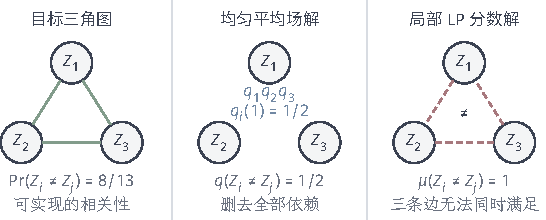
\includegraphics[width=92.445mm]{figures/09-probabilistic-graphical-models/02-inference/tikz/pgm-variational-triangle/figure.pdf}
  \caption{三角图、完全因子化分布和局部一致的边缘表。中间为本例均匀平均场解$q_i(Z_i=1)=1/2$，其边异值概率为$1/2$。右侧让每条边都以概率$1$取不同值，节点边缘仍都是$(1/2,1/2)$；它满足局部一致性，却不可能由任何全局二元分布实现。}
  \label{fig:pgm-variational-triangle}
\end{figure}

\section{近似后验分布与边缘概率}

\label{sec:pgm-variational-posterior}

后验分布或边缘概率难以精确求出时，需要回答三个问题：怎样构造可计算的近似，怎样求出这个近似，以及它能否可靠地回答所需的查询。下面依次讨论后验分布与边缘概率的近似、近似的计算和近似的可靠性。

\subsection{后验分布与边缘概率的近似}
\label{sec:pgm-variational-laplace-ep}

限制全局分布、放宽局部边缘的一致性、匹配分布矩和近似局部曲率，改变的是不同的概率对象与近似准则。各方法的更新公式在构造中一并给出；随后再讨论如何组织这些计算。

\subsubsection{基于因子化分布的近似}

\label{sec:pgm-variational-mean-field}
\label{sec:pgm-variational-mean-field-structured}
\label{sec:pgm-variational-coordinate}

完整联合概率表要记录每一种变量组合，$d$个二元变量就需要$2^d-1$个自由概率，这正是精确推断扛不住的原因。最简单的“砍参数”办法是假设推断时各变量\emph{相互独立}：只保存每个变量自己的边缘分布（$d$个二元变量只需$d$个数），再把它们相乘当作联合分布。这样做当然丢掉了变量之间的相关性——但原模型里的耦合并没有消失，它会在逐个更新某个变量时、通过“其他变量的期望”重新进入计算。\term{平均场近似}（mean-field approximation）采用
\[
  q(\bm{z})=\prod_{i=1}^{d}q_i(z_i).
\]
在$q$中，各变量相互独立，条件分布因而不随其他变量的取值改变。原模型的耦合仍通过期望进入坐标更新，因子化简化的是近似分布的表达。

因子化之后，仍要选择各个$q_i$，使整个乘积分布的ELBO尽量大。可以先保持其他因子不变，只调整一个$q_i$，再依次轮换；这相当于把一次联合优化拆成多次单因子优化。这里固定的是其他变量的分布，而非其他变量的某个取值。记$q_{-i}=\prod_{j\ne i}q_j$，并定义$a_i(z_i)=\mathbb E_{q_{-i}}\log p(\bm{x},z_i,\bm{Z}_{-i})$。ELBO中依赖$q_i$的部分为
\[
  \int q_i(z_i)a_i(z_i)\,dz_i-\int q_i(z_i)\log q_i(z_i)\,dz_i.
\]
假设$C_i=\int e^{a_i(z_i)}dz_i$有限且为正，令$q_i^\star=e^{a_i}/C_i$，上述表达式就等于$\log C_i-\operatorname{KL}(q_i\Vert q_i^\star)$。KL在两分布相同时取唯一最小值，因此得到最优坐标更新：
\begin{equation}
  q_i^\star(z_i)
    \propto\exp\left\{\mathbb E_{q_{-i}}
      [\log p(\bm{x},z_i,\bm{Z}_{-i})]\right\}.
  \label{eq:pgm-variational-coordinate}
\end{equation}
期望只对其他变量计算，$z_i$在这一步是保留的自变量。更新使用的是对数联合分布的期望，再取指数；一般不等于$\mathbb E_{q_{-i}}p(z_i\mid\bm{x},\bm{Z}_{-i})$，也不等于把其他变量一律替换为其均值。

若原模型按因子分解，所有不含$z_i$的项都是归一化时可去掉的常数。平均场因此仍能局部更新。对例~\ref{ex:pgm-variational-triangle}，现在直接使用未归一化得分$S_\beta$，定义对数配分函数下界
\begin{equation}
  \begin{aligned}
    \mathcal L_Z(q)&=\mathbb E_qS_\beta(\bm Z)+H(q),\\
    \operatorname{KL}(q\Vert p_\beta)
      &=\log Z_\beta-\mathcal L_Z(q).
  \end{aligned}
  \label{eq:pgm-variational-partition-lower-bound}
\end{equation}
因此$\mathcal L_Z(q)\leq\log Z_\beta$。若使用已归一化的$p_\beta$计算$\mathbb E_q\log p_\beta+H(q)$，结果则是$\mathcal L_Z(q)-\log Z_\beta\leq0$，两者相差一个与$q$无关的常数。

令$m_i=q_i(Z_i=1)$。在乘积分布中，两节点取不同值分为互斥的两种情况：$Z_i=1,Z_j=0$与$Z_i=0,Z_j=1$。由独立性，它们的概率之和为
\[
  q(Z_i\ne Z_j)
    =m_i(1-m_j)+(1-m_i)m_j
    =m_i+m_j-2m_im_j.
\]
每条边的期望得分就是这个概率乘以$\beta$。乘积分布的熵等于各伯努利熵之和；记$h_{\mathrm B}(m)=-m\log m-(1-m)\log(1-m)$，并按连续延拓约定$h_{\mathrm B}(0)=h_{\mathrm B}(1)=0$。将得分与熵合并，并记$\mathcal L_{\mathrm{MF}}(\bm m)=\mathcal L_Z(\prod_iq_i)$，便得到下面第一行的目标；第二行是由它求出的坐标更新：
\begin{equation}
  \begin{aligned}
    \mathcal L_{\mathrm{MF}}(\bm m)
      &=\beta\sum_{(i,j)\in E}
           (m_i+m_j-2m_im_j)+\sum_i h_{\mathrm B}(m_i),\\
    m_i^{\mathrm{new}}
      &=\sigma\left(\beta\sum_{j\in N(i)}(1-2m_j)\right),
  \end{aligned}
  \label{eq:pgm-variational-triangle-mf}
\end{equation}
其中$\sigma(u)=1/(1+e^{-u})$，$N(i)$是相邻节点集合。为了看清第二行的来源，固定其他$m_j$，对第一行关于$m_i$求导：
\[
  \frac{\partial\mathcal L_{\mathrm{MF}}}{\partial m_i}
    =\beta\sum_{j\in N(i)}(1-2m_j)
       +\log\frac{1-m_i}{m_i}.
\]
令该导数为零并移项，就得到$\log\{m_i/(1-m_i)\}=\beta\sum_{j\in N(i)}(1-2m_j)$。解出$m_i$，正是式~\eqref{eq:pgm-variational-triangle-mf}中的坐标更新。若两个邻居的$m_j$均为$1/4$，两项$(1-2m_j)$之和为$1$，新$m_i=\sigma(\log2)=2/3$；邻居偏好$0$，当前变量便更偏好$1$。更新后的$m_i$仍表示伯努利分布中的概率，保留当前变量的不确定性。

均匀初始化给出固定点$m_i=1/2$，因为每个$(1-2m_j)$都为零，更新仍返回$\sigma(0)=1/2$。此时三条边各以概率$1/2$取不同值，期望得分为$3\beta/2$；三个节点各贡献熵$\log2$。因此其对数配分函数下界为$\mathcal L_{\mathrm{MF}}=(9/2)\log2\approx3.119162$，低于$\log26\approx3.258097$。

这一例中，均匀固定点还是平均场的唯一全局最优点。先在$0<m_i<1$内计算目标Hessian：对角元为$-1/[m_i(1-m_i)]\leq-4$，相邻两节点对应的非对角元为$-2\beta$。三角图中每行恰有两个这样的非对角元，所以对任意向量$\bm u$，利用$2|u_i u_j|\leq u_i^2+u_j^2$可得
\[
  \bm u^\top\nabla^2\mathcal L_{\mathrm{MF}}\bm u
    \leq(-4+4\beta)\lVert\bm u\rVert_2^2.
\]
这里$\beta=\log2<1$，故最大特征值不超过$-4+4\beta<0$，目标在内部严格凹。

还须排除最大值出现在边界的可能。固定其他节点时，得分关于$m_i$是斜率有限的线性函数，而伯努利熵的导数$\log\{(1-m_i)/m_i\}$在$m_i\to0$时趋于$+\infty$，在$m_i\to1$时趋于$-\infty$。因此从任一端点向内部移动足够小的距离，都能增加目标。目标在闭立方体$[0,1]^3$上连续，最大值存在；边界不能取最大值，内部严格凹且均匀点的梯度为零，所以均匀点就是唯一全局最大点。

即使如此，该最优乘积分布仍给出$q(Z_i\ne Z_j)=1/2$，低于真实的$8/13$。这一差距来自独立近似族的表达限制，即使达到其全局最优仍会保留。

\par\noindent\begin{minipage}{\linewidth}
\begin{algorithm}[循环坐标平均场]
  \label{alg:pgm-variational-cavi}
  \begin{algorithmic}[1]
    \Require 联合分布、因子化近似族、有限ELBO的初值$q$、可归一化的坐标更新、容差$\varepsilon>0$、最大轮数$T_{\max}\in\mathbb N_{>0}$
    \Ensure 近似分布$q$及其ELBO
    \State 计算当前ELBO，令轮数$t\gets0$
    \Repeat
      \State 保存本轮开始时的ELBO
      \For{$i=1,\ldots,d$}
        \State 用其他因子的最新值计算式~\eqref{eq:pgm-variational-coordinate}
        \State 归一化并替换$q_i$
      \EndFor
      \State 重新计算ELBO及本轮增量，令$t\gets t+1$
    \Until{增量不超过$\varepsilon$，或$t\geq T_{\max}$}
  \end{algorithmic}
\end{algorithm}
\end{minipage}\par

算法~\ref{alg:pgm-variational-cavi}将一遍完整坐标扫描记为一轮，以$T_{\max}$给出计算预算。停止时输出的是当前近似分布；达到预算本身不表示目标增量已经小于容差。算法依次使用其他因子的最新值，精确最大化每个坐标。因此，把同一更新持续执行时，ELBO单调不减，又以对数证据为上界，目标值序列收敛。参数序列收敛和一般模型的全局最优还需要其他条件。同时使用旧值并行更新所有坐标时，更新之间相互影响，上述逐坐标单调性论证不适用。

完全独立的平均场有时砍得太狠——比如一条隐藏状态链上相邻状态高度相关，硬把它们当独立会丢掉最关键的轨迹协调关系。一个折中是\emph{有选择地}在近似分布$q$里保留一部分依赖：把变量分成若干块，块与块之间独立，块内部仍做（可能精确的）联合推断。这样表达力比完全平均场强，代价是每块的更新更贵。单变量因子化会拆开后验中的重要依赖。例如，相邻隐状态高度相关时，独立边缘无法表达一条轨迹上状态选择的协调关系。\term{结构化变分推断}（structured variational inference）在$q$中保留选定的依赖，通过块内推断计算相关状态的联合概率。表达能力由此增强，局部更新的成本也随之增加。
\label{sec:pgm-variational-structured}

一种直接选择是把节点划分成互不相交的块$B_1,\ldots,B_K$，并让不同块独立，即
\[
  q(\bm z)=\prod_k q_k(\bm z_{B_k}).
\]
与单变量推导相同，固定其余块后，当前块的最优分布满足
\begin{equation}
  q_k^\star(\bm z_{B_k})
     \propto\exp\left\{
       \mathbb E_{q_{-B_k}}\log p(\bm x,\bm z_{B_k},\bm Z_{-B_k})
     \right\}.
  \label{eq:pgm-variational-block}
\end{equation}
块内部原有相互作用被保留，跨块作用转成期望势。链与小树都可以沿用第~\ref{sec:pgm-junction-tree-sum-product}节的和积消息；在链上向两个方向传递消息，就是后文时序模型使用的前向--后向计算。若是稠密大块，更新仍会遇到指数级枚举。因此，块大小只是粗略指标，块内树宽和因子的代数结构才决定计算代价。

回到三角图，取$q(z_1,z_2)q(z_3)$并令$q(z_3=1)=1/2$。固定任一$z_1,z_2$时，均匀的$Z_3$与$z_1$取不同值的概率是$1/2$，与$z_2$取不同值的概率也是$1/2$。因此对$Z_3$求期望后，两条跨块边的得分总和恒为$\beta$，不会改变块$(Z_1,Z_2)$内各配置的相对权重。块内得分仍为$\beta\mathbb I[z_1\ne z_2]$，将四个配置的权重归一化便得
\[
  q(z_1,z_2)=
    \frac{e^{\beta\mathbb I[z_1\ne z_2]}}{2+2e^\beta}.
\]
记$C=2+2e^\beta$。两个异值配置的总权重是$2e^\beta$，所以当$\beta=\log2$时，块内不同值的概率为$2e^\beta/C=2/3$。同时翻转$Z_1,Z_2$不会改变块分布，因此两个节点的边缘仍均为$(1/2,1/2)$。反过来更新$q(z_3)$时，这两个均匀边缘使两条跨块边对任一固定$z_3$的期望得分都为$\beta/2$；总得分不随$z_3$改变，更新仍返回均匀分布。这样就验证了两个方向的块坐标更新都不再改变当前解，故它是块坐标固定点。两条跨块边的不同值概率仍为$1/2$。

为了计算这一近似给出的下界，对块分布的对数取期望，得到
\[
  H(q_{1,2})=\log C-\beta q(Z_1\ne Z_2).
\]
块内期望得分为$\beta q(Z_1\ne Z_2)$，恰好与上式第二项相消。再加上跨块期望得分$\beta$和$q_3$的熵$\log2$，便有$\mathcal L_Z=\log(2+2e^\beta)+\beta+\log2=\log24\approx3.178054$。这个下界高于完全平均场的$3.119162$，但仍低于$\log26$。与完全平均场相比，块内联合分布提高了该下界，但两条跨块边的相关性仍未进入$q$。

若$\mathcal Q_1\subseteq\mathcal Q_2$，对同一ELBO有$\sup_{\mathcal Q_1}\mathcal L\leq\sup_{\mathcal Q_2}\mathcal L$；这一关系比较的是近似族中的最优目标值。有限预算下的实际解还受优化误差影响。更一般的树结构$q$未必能分成互不相交的块，可以用树边缘及条件分布参数化，其熵仍能精确计算。这些结构均需定义合法的全局$q$，并正确计算期望和真实熵，才能继续使用ELBO下界。结构化变分补回了选定依赖，却提高了每次坐标更新的成本。若直接维护全局分布仍然困难，还可以改变近似对象，只维护局部概率表；下面考察这种安排。

\subsubsection{基于局部边缘的近似}

\label{sec:pgm-variational-bethe-kikuchi}
\label{sec:pgm-variational-local-free-energy}
\label{sec:pgm-variational-bethe}

平均场和结构化变分都还是先构造一个合法的全局分布$q$，只是限制了它的形式。另一个更激进的思路是\emph{干脆不构造全局$q$}，直接维护我们最终真正想要的那些局部概率表（每个变量的边缘、每个因子上的联合边缘），让它们在重叠处彼此一致，然后用第6章的和积消息在含环图上\emph{反复}迭代——这就是环置信传播。它在树上精确，在环上是近似，而且这些局部表未必能拼成同一个全局分布，因此被谨慎地称为“伪边缘”。结构化平均场把部分依赖保存在一个合法$q$中。另一种思路是不先构造全局$q$，而是直接维护节点和因子的局部概率表。以下设有限离散因子图的目标为$p(\bm z)=Z^{-1}\prod_a\psi_a(\bm z_{S_a})$，所有因子严格正，每个变量至少邻接一个因子。观测已吸收到$\psi_a$中。令$N(i)$为变量$i$的邻接因子集合，$d_i=|N(i)|$。树上的和积消息是
\begin{equation}
  \begin{aligned}
    n_{i\to a}(z_i)
      &\propto\prod_{b\in N(i)\setminus\{a\}}m_{b\to i}(z_i),\\
    m_{a\to i}(z_i)
      &\propto\sum_{\bm z_{S_a\setminus\{i\}}}
            \psi_a(\bm z_{S_a})
            \prod_{j\in S_a\setminus\{i\}}n_{j\to a}(z_j).
  \end{aligned}
  \label{eq:pgm-variational-lbp}
\end{equation}
树上去掉一条边会分离两个子图，因此消息汇总的是互不重复的变量集合；完整的双向传递可得精确边缘。在含环图上照用同一更新，就是\term{环置信传播}（loopy belief propagation, LBP）。环使传回的信息可能已经受过当前节点的影响，树上的独立分支解释随之失效。

算法从消息读出
\[
  b_i(z_i)\propto\prod_{a\in N(i)}m_{a\to i}(z_i),
  \qquad
  b_a(\bm z_{S_a})\propto\psi_a(\bm z_{S_a})
                         \prod_{i\in S_a}n_{i\to a}(z_i).
\]
这些$b_i,b_a$称为\term{伪边缘}（pseudomarginal）：它们被当成边缘概率使用，但暂未保证存在一个共同的全局分布。将非负、归一化及
\begin{equation}
  \sum_{\bm z_{S_a\setminus\{i\}}}b_a(\bm z_{S_a})=b_i(z_i),
  \qquad i\in S_a
  \label{eq:pgm-variational-local-consistency}
\end{equation}
组成的约束集合记为$\mathcal L$，称为\term{局部多面体}（local polytope）。它只检查因子与节点是否一致，故$\mathcal M\subseteq\mathcal L$；在含环图上包含关系可能严格。

每个因子熵已经包含其中节点的熵，因此直接相加需要校正重复计数。树结构恰好允许减掉多算的部分：
\begin{equation}
  \begin{aligned}
    H_{\mathrm B}(\bm b)
      &=\sum_aH(b_a)+\sum_i(1-d_i)H(b_i),\\
    F_{\mathrm B}(\bm b)
      &:=-\sum_a\mathbb E_{b_a}\log\psi_a-H_{\mathrm B}(\bm b).
  \end{aligned}
  \label{eq:pgm-variational-bethe}
\end{equation}
$F_{\mathrm B}$是\term{Bethe自由能}（Bethe free energy），即负的期望对数得分再减去局部熵近似。最小化自由能等价于最大化相应的得分加熵，其中使用的是局部熵近似，在一般含环图上未必对应合法$q$的真实熵。

在树上，可以通过构造全局分布验证熵公式的精确性。对正的局部一致$\bm b$，构造
\[
  q_{\mathrm T}(\bm z)=
    \frac{\prod_a b_a(\bm z_{S_a})}
         {\prod_i b_i(z_i)^{d_i-1}}.
\]
从叶端向内求和时，每次用局部一致性消去一个分支，最终得到$1$；保留任一节点或因子而消去其余分支，就得到对应的$b_i$或$b_a$。对$\log q_{\mathrm T}$求期望给出$H(q_{\mathrm T})=H_{\mathrm B}(\bm b)$。任何具有相同局部边缘的分布$q$都满足$\mathbb E_q\log q_{\mathrm T}=\mathbb E_{q_{\mathrm T}}\log q_{\mathrm T}$，于是$\operatorname{KL}(q\Vert q_{\mathrm T})=H_{\mathrm B}(\bm b)-H(q)\geq0$。因此$H_{\mathrm B}$正是这些边缘下的最大熵，$\mathcal L=\mathcal M$，式~\eqref{eq:pgm-variational-gibbs}适用。含零边缘的树情形可由条件分布构造或取极限处理；含环图无法通过消叶分离全部分支，这一精确性论证限于树结构。

\begin{theorem}[正消息固定点与Bethe驻点]
  \label{thm:pgm-variational-bp-stationary}
  设有限因子图中的每个变量具有有限非空状态空间且至少邻接一个因子，每个因子$\psi_a$均取有限严格正值。令$\mathcal L$为由非负性、归一化及式~\eqref{eq:pgm-variational-local-consistency}定义的局部多面体，$F_{\mathrm B}$为式~\eqref{eq:pgm-variational-bethe}定义的Bethe自由能。按任一固定正归一化约定，LBP正消息固定点所产生的伪边缘是$F_{\mathrm B}$在$\mathcal L$相对内部的驻点。反之，$\mathcal L$中的每个正内部驻点都能由一组满足式~\eqref{eq:pgm-variational-lbp}的正消息表示，消息的正比例缩放不影响伪边缘。
\end{theorem}
\begin{proof}
  我们先从自由能驻点构造消息，再验证消息固定点满足同一组驻点条件。正内部的非负约束尚未激活，只需处理归一化与局部一致性。为约束$\sum_{\bm z_{S_a\setminus\{i\}}}b_a-b_i=0$引入乘子$\lambda_{a,i}(z_i)$，为每张表的归一化引入$\alpha_a,\alpha_i$。完整的拉格朗日函数为
  \[
    \begin{aligned}
      \mathscr J={}&F_{\mathrm B}(\bm b)
        +\sum_a\alpha_a\left[\sum_{\bm z_{S_a}}b_a-1\right]\\
       &+\sum_i\alpha_i\left[\sum_{z_i}b_i-1\right]\\
       &+\sum_a\sum_{i\in S_a}\sum_{z_i}\lambda_{a,i}(z_i)
          \left[\sum_{\bm z_{S_a\setminus\{i\}}}
                         b_a(\bm z_{S_a})-b_i(z_i)\right].
    \end{aligned}
  \]
  对因子表和节点表分别求偏导。由于$\partial(b\log b)/\partial b=\log b+1$，两类方程为
  \[
    \begin{aligned}
      0={}&\log b_a-\log\psi_a+1
                    +\sum_{i\in S_a}\lambda_{a,i}+\alpha_a,\\
      0={}&(1-d_i)(\log b_i+1)
                    -\sum_{a\in N(i)}\lambda_{a,i}+\alpha_i.
    \end{aligned}
  \]
  因子表方程中的$1+\alpha_a$不依赖配置，可并入归一化常数。令$n_{i\to a}=e^{-\lambda_{a,i}}>0$，得到
  \[
    b_a\propto\psi_a\prod_{i\in S_a}n_{i\to a},
    \qquad n_{i\to a}=e^{-\lambda_{a,i}}.
  \]
  节点表方程则给出$(1-d_i)\log b_i-\sum_a\lambda_{a,i}=\text{常数}$。移项并取指数，可写成
  \[
    \prod_{a\in N(i)}n_{i\to a}(z_i)
       \propto b_i(z_i)^{d_i-1}.
  \]
  定义$m_{a\to i}$为式~\eqref{eq:pgm-variational-lbp}第二行的求和。把$b_a$向$z_i$边缘化时，$n_{i\to a}(z_i)$与被求和的变量无关，可移到求和号外；局部一致性因此给出$b_i\propto n_{i\to a}m_{a\to i}$。对$a\in N(i)$连乘，便有
  \[
    b_i^{d_i}\propto
       \left(\prod_a n_{i\to a}\right)
       \left(\prod_a m_{a\to i}\right)
      \propto b_i^{d_i-1}\prod_a m_{a\to i}.
  \]
  每个$b_i(z_i)>0$，所以可以约去$b_i^{d_i-1}$，得到$b_i\propto\prod_a m_{a\to i}$。再代回任一$b_i\propto n_{i\to a}m_{a\to i}$，约去正的$m_{a\to i}$，便得$n_{i\to a}\propto\prod_{b\ne a}m_{b\to i}$，即第一行消息方程。这里没有除以$d_i-1$；度为$1$时，被约去的是$b_i^0=1$，所以推导也覆盖叶节点。

  反过来，给定正消息固定点，先按定理前的读出公式将$b_a,b_i$分别归一化。因子消息更新使$b_a$对其余变量求和后正比于$n_{i\to a}m_{a\to i}$，变量消息更新又使这一乘积正比于$\prod_b m_{b\to i}$；两张归一化的节点表因而相等，局部一致性成立。将$n_{i\to a}\propto\prod_{b\ne a}m_{b\to i}$对$a$连乘，每条$m_{b\to i}$恰出现$d_i-1$次，所以$\prod_a n_{i\to a}\propto b_i^{d_i-1}$也成立。取$\lambda_{a,i}=-\log n_{i\to a}$，便恢复两类驻点方程中依赖状态的部分；剩余与状态无关的常数由$\alpha_a,\alpha_i$吸收，即满足全部驻点条件。
\end{proof}

定理建立了固定点与驻点的对应。驻点可能是局部极小点、鞍点或退化点，一般含环图的Bethe熵也未必凹。普通LBP迭代还可能振荡，或从不同初值到达不同固定点。为减小一次更新对当前消息的改变，可以先用当前邻居消息按LBP规则算出正的候选$\widetilde m$，再取$0<\gamma\leq1$，作阻尼更新
\[
  \log m^{\mathrm{new}}\leftarrow
      (1-\gamma)\log m^{\mathrm{old}}+\gamma\log\widetilde m.
\]
这一步先在对数尺度上混合旧消息与候选，再指数化，并按所选消息规范归一化；$\gamma=1$恢复未阻尼更新，较小的$\gamma$保留更多旧消息。阻尼可以减轻某些振荡，普遍收敛仍需要额外条件。硬约束产生零概率时，还需处理边界和消息比值的定义。固定点与自由能关系的原始论证见Yedidia等人\scite{pgm-variational-yedidia2005}。

三角图的均匀消息固定点仍有边缘误差。先保留一般$\beta$并令$r=e^\beta>0$，边势表的同值项为$1$、异值项为$r$。每行的和都等于$1+r$，所以输入均匀消息后，对任一端点状态求出的新消息仍相同；归一化后依旧是均匀消息，确为固定点。读出公式给出$b_i=(1/2,1/2)$，边表则只需归一化势表：两个同值项各为$1/[2(1+r)]$，两个异值项各为$r/[2(1+r)]$。当$r=2$时，$b_{i,j}(0,1)=b_{i,j}(1,0)=1/3$，$b_{i,j}(0,0)=b_{i,j}(1,1)=1/6$。边上不同值的概率$2/3$不同于真实的$8/13$。

为了计算这个固定点的自由能，注意每条边的期望对数得分为$\beta r/(1+r)$，边熵为
\[
  H(b_{i,j})=\log[2(1+r)]-\frac{r}{1+r}\log r,
  \qquad H(b_i)=\log2.
\]
三角图每个节点的度为$2$，因此Bethe熵要从三个边熵之和中减去三个节点熵。将期望得分也加回来，并用$\beta=\log r$，得到
\[
  \begin{aligned}
    -F_{\mathrm B}
      &=3\frac{r\log r}{1+r}
        +3\left\{\log[2(1+r)]
                     -\frac{r\log r}{1+r}\right\}\\
      &\qquad-3\log2\\
      &=3\log(1+r).
  \end{aligned}
\]
当$r=2$时，$-F_{\mathrm B}=3\log3=\log27>\log26$，所以它不是对数配分函数下界。

这个例子还能检验界方向。在上面$\beta$为任意实数、$r=e^\beta>0$的模型中，同一均匀固定点给出$Z_{\mathrm B}=(1+r)^3$，精确值是$Z=2+6r^2$，二者相差$(r-1)^3$。当$r=2$时Bethe高估，当$r=1/2$时$Z_{\mathrm B}=27/8<7/2=Z$，则低估。两种情形中的节点边缘都仍然精确。这说明节点边缘的正确性与配分函数、联合依赖的误差是不同的诊断结果。

\label{sec:pgm-variational-kikuchi}

Bethe近似只维护节点和因子这两级小表，因此无法捕捉“短环上几个因子\emph{共同}施加的约束”——三角图里三条边必须同时满足的那种闭合关系，就被拆开看丢了。改进办法是把作用域扩大：直接维护覆盖短环（如网格的一个小方格）的\emph{大区域}联合表，再让大区域在重叠的交集上保持边缘一致，并仔细用“计数数”抵消重复计数。这就是Kikuchi（聚类）近似与广义置信传播。三角图中的边表可以分别满足节点一致性，却遗漏三条边共同闭合的约束。Bethe只维护节点和原因子作用域上的伪边缘，因而无法直接检查这一短环关系。Kikuchi近似扩大表格的作用域：维护覆盖短环的联合表格，再使重叠区域上的边缘一致。这里的\term{区域}（region）包含一组变量及分配给它的模型因子，区域大小决定一次能够检查哪些联合关系。

一种标准构造从覆盖全部原因子的最大区域出发，加入所需非空交集，形成按包含关系连接的有向无环区域图。用$R$表示区域的变量集合，$b_R$是其归一化伪边缘。对父区域$R$及子区域$S\subset R$要求$\sum_{\bm z_{R\setminus S}}b_R=b_S$。每个区域的\term{计数数}（counting number）$c_R$纠正重叠造成的重复计数；对按包含关系闭合的构造，可递归设
\begin{equation}
  c_R=1-\sum_{R'\supsetneq R}c_{R'}.
  \label{eq:pgm-variational-counting}
\end{equation}
这一构造要求每个原变量和原因子在覆盖它的区域中的计数总和为$1$，且涉及同一变量或因子的区域通过相应包含边连通。覆盖、计数和连通条件共同确定可使用的区域近似。

令$\Theta_R(\bm z_R)=\sum_{a:S_a\subseteq R}\log\psi_a(\bm z_{S_a})$，并假设上述因子计数条件成立，则
\begin{equation}
  \begin{aligned}
    H_{\mathrm K}(\bm b)&=\sum_R c_R H(b_R),\\
    F_{\mathrm K}(\bm b)
      &=\sum_R c_R\left[
          \sum_{\bm z_R}b_R(\bm z_R)\log b_R(\bm z_R)
          -\mathbb E_{b_R}\Theta_R\right].
  \end{aligned}
  \label{eq:pgm-variational-kikuchi}
\end{equation}
这是\term{Kikuchi自由能}（Kikuchi free energy）的一种区域表示。因子计数和区域一致性使能量项仍把每个原因子计算一次，近似发生在熵及全局一致性上。若不同因子作用域至多共享一个变量，Bethe对应只用因子区域和单节点区域的特殊选择。一般因子图的Bethe仍属于区域自由能，但当因子共享多个变量时，未必等同于上述按全部交集闭合的Kikuchi构造。Kikuchi通过更大的联合表格和交集约束检查短环关系，消息的作用域也随之扩大。

例如，在$3\times3$节点网格中选择四个小方格为最大区域，如图~\ref{fig:pgm-variational-regions}。将左上、右上、左下、右下的方格依次记为$A,B,C,D$。四个方格的非空交集去重后，只有四条共享内部边$e_{A,B},e_{A,C},e_{B,D},e_{C,D}$及中央节点$o$；其中$e_{A,B}=A\cap B$，其余记号同理。四个方格各计$+1$；两方格共享的四条内部边各计$1-1-1=-1$；中央节点被四个方格及四条内部边共同覆盖，故还需计$1-4+4=+1$。相应熵为“四个方格熵之和，减四条内部边熵，再加中央节点熵”。若各节点独立且熵均为$h$，它给出$4(4h)-4(2h)+h=9h$，恰好没有重复计算任何节点。这个计算验证了独立情形中的计数。相关分布的联合熵还涉及这些局部表格之外的依赖。

网格的外边界边不属于上述四个方格之间的非空交集。若为记录边表而额外保留它们，就得到冗余子区域。例如，最上方左侧的外边只被$A$覆盖，其计数为$1-c_A=0$。它的表可直接由$b_A$边缘化得到；再保留该边上的外角节点时，该节点的计数也为$1-c_A-0=0$，其表由同一条边继续边缘化即可。这类零计数区域不增加熵项，可以保留作显式一致性约束；只有在删除后仍能通过已有约束得到相同的边缘关系时，才可省去它们。下面的消息示例使用四方格、四内部边和中央点组成的区域图，不额外加入这些外边界子区域。

\begin{figure}[htbp]
  \centering
  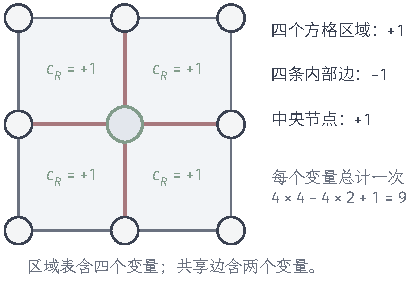
\includegraphics[width=70.831mm]{figures/09-probabilistic-graphical-models/02-inference/tikz/pgm-variational-regions/figure.pdf}
  \caption{四方格区域近似的计数。浅色块表示四个计数为$+1$的四变量区域，粗线标出四个计数为$-1$的共享内部边区域，中央节点区域的计数为$+1$。外边界线是原网格边，不表示本构造额外维护了外边界区域。每条区域一致性约束都要求大表格向子区域边缘化后与小表格相同；颜色之外还用区域面积、线条和节点区分三个层次。}
  \label{fig:pgm-variational-regions}
\end{figure}

区域消息可以由自由能的约束驻点条件导出。对约束$\sum_{\bm z_{R\setminus S}}b_R-b_S=0$引入乘子$\lambda_{R,S}(\bm z_S)$。对某张$b_R$求导时，$R$作为父区域产生正的出边乘子，作为子区域产生负的入边乘子；将它们移到等式右侧，内部驻点满足
\begin{equation}
  c_R(\log b_R-\Theta_R)
    =\sum_{P:\,P\to R}\lambda_{P,R}
       -\sum_{S:\,R\to S}\lambda_{R,S}+\text{常数}.
  \label{eq:pgm-variational-region-stationarity}
\end{equation}
归一化项及$c_R$带来的常数已经合并。每个乘子都是子区域配置上的函数，用来协调父、子两张表；因此它的指数可以作为正的校正因子。不过，直接指数化这里的$\lambda_{R,S}$，通常不能得到下面标准父子形式中的同名边消息，因为驻点方程还含$c_R$，同一约束也可能有冗余表示。需要先把一致性约束重新组合，再给新乘子取指数。消息以整个子区域的配置为索引，负计数区域的校正还会在更新中产生分母，计算对象因此比单节点消息更大。$c_R=0$时，上式只给出乘子之间的约束，不能除以$c_R$来求$b_R$；这一约束及原有的边缘一致性都应保留。

为说明计数怎样进入这种重组，记$\mathcal A(R)$为$R$的严格祖先集合，$b_A^{\downarrow S}$为将$b_A$向$S$边缘化所得的表。对一条父子边$P\to S$，考察加权约束
\begin{equation}
  G_{P,S}:=c_Sb_S+
    \sum_{A\in\mathcal A(S)\setminus(\{P\}\cup\mathcal A(P))}
         c_A b_A^{\downarrow S}=0.
  \label{eq:pgm-variational-region-weighted-constraint}
\end{equation}
原有的逐边一致性保证其中每张祖先表都边缘化为$b_S$。又因为区域及其全部祖先的计数之和为$1$，将$S$与$P$的这两个计数恒等式相减，便得
\[
  c_S+
    \sum_{A\in\mathcal A(S)\setminus(\{P\}\cup\mathcal A(P))}
      c_A=0.
\]
因此$G_{P,S}=0$确实是原一致性约束的线性组合。在四方格例中，边区域$S=e_{A,B}$只有两个祖先$A,B$，而$c_S=-1,c_A=c_B=1$，所以$G_{A,S}=0$就是$-b_S+b_B^{\downarrow S}=0$，$G_{B,S}=0$则是$-b_S+b_A^{\downarrow S}=0$。两条约束交换了原来分别协调的父区域，负计数已包含在这个组合中。

在当前四方格这种所有保留区域计数均非零的有效构造中，还能反向恢复原一致性。具体地，从最大区域向下归纳，设当前子区域$S$上方的表已经一致，记$v_S=c_Sb_S+\sum_{A\in\mathcal A(S)}c_A b_A^{\downarrow S}$。对任一父区域$P$，$P$及其祖先的计数和为$1$，而相应表已与$b_P$一致，所以$G_{P,S}=0$给出$v_S=b_P^{\downarrow S}$。各父表在$S$上的边缘因而相同，所有祖先的边缘也都等于$v_S$。将这一结果代回$v_S$的定义，得到$v_S=c_Sb_S+(1-c_S)v_S$；由$c_S\ne0$即得$b_S=v_S=b_P^{\downarrow S}$。重组约束因而不改变这些表所需满足的边缘关系。

为把这些约束写成消息，记$\mathcal D(R)$为$R$及其全部后代，$\partial R$为所有从$\mathcal D(R)$外进入$\mathcal D(R)$的有向区域边。在每个子区域配置上，以$-\xi_{P,S}(\bm z_S)$作为$G_{P,S}=0$的乘子。一个$G_{P,S}$含$b_R$，恰好意味着$S=R$，或$S$是$R$的后代而$P$在$\mathcal D(R)$外；其中$b_R$的系数都是$c_R$。因此，对非零计数区域$R$求导，约束项的贡献为$-c_R\sum_{(P\to S)\in\partial R}\xi_{P,S}$，既包括进入$R$的边，也包括从外部进入其后代的边。将它与自由能导数合并并除以$c_R$，驻点条件就写成$\log b_R=\Theta_R+\sum_{\partial R}\xi_{P,S}+\text{常数}$。取$m_{P\to S}=e^{\xi_{P,S}}$，才得到下面的边界消息表示。

含零计数区域时，上面的反推步骤不能除以$c_S$，加权约束也可能退化，故仍须保留原父子一致性，并由父表边缘确定这些区域的表；有多个父区域时，还要检查它们给出的边缘相同。不能从一条除以零的驻点式定义零计数表。一般有效区域图的父子参数化与驻点关系见Yedidia等人\scite{pgm-variational-yedidia2005}。

在标准父子区域参数化中，还能把消息方程写成可直接计算的形式。令$\Psi_R=e^{\Theta_R}$，伪边缘写为
\[
  b_R(\bm z_R)\propto
    \Psi_R(\bm z_R)
       \prod_{(P\to Q)\in\partial R}m_{P\to Q}(\bm z_Q).
\]

这里$\partial R$中的每条边都终止于$R$或其某个子区域，故相应消息只依赖$\bm z_R$内的变量。例如，四方格区域图只连接方格到其内部边、内部边到中央点。对$R=A$及$S=e_{A,B}$，后代集合及外部入边分别为
\[
  \begin{aligned}
    \mathcal D(A)&=\{A,e_{A,B},e_{A,C},o\},\\
    \partial A&=\{B\to e_{A,B},\ C\to e_{A,C},\\
              &\qquad e_{B,D}\to o,\ e_{C,D}\to o\},\\
    \mathcal D(S)&=\{S,o\},\\
    \partial S&=\{A\to S,\ B\to S,\ e_{A,C}\to o,\\
              &\qquad e_{B,D}\to o,\ e_{C,D}\to o\}.
  \end{aligned}
\]
例如$e_{B,D}\to o$进入了$A$的后代中央点，虽然没有直接进入$A$，仍须出现在$b_A$中。这些入边组合承担了计数校正，不能只保留直接指向当前区域的消息。

再把消息表示代入父子一致性。设$C_R,C_S>0$分别为两张表的归一化常数，则
\[
  \frac{1}{C_R}\sum_{\bm z_{R\setminus S}}
        \Psi_R\prod_{\partial R}m
    =\frac{1}{C_S}\Psi_S\,m_{R\to S}
        \prod_{\partial S\setminus\{R\to S\}}m.
\]
将除$m_{R\to S}$以外的子区域项移到分母，且将与$\bm z_S$无关的$C_S/C_R$吸收到消息归一化中，得到更新方程
\begin{equation}
  m_{R\to S}(\bm z_S)\propto
  \frac{\displaystyle
    \sum_{\bm z_{R\setminus S}}
      \Psi_R(\bm z_R)
       \prod_{(P\to Q)\in\partial R}m_{P\to Q}(\bm z_Q)}
  {\displaystyle
    \Psi_S(\bm z_S)
       \prod_{\substack{(P\to Q)\in\partial S\\(P\to Q)\ne(R\to S)}}
          m_{P\to Q}(\bm z_Q)}.
  \label{eq:pgm-variational-gbp}
\end{equation}

同时出现在分子、分母且只依赖$\bm z_S$的项可先约去；若还依赖被求和的变量，就不能移出求和号约去。上面的四方格例中，$m_{B\to S}$、$m_{e_{B,D}\to o}$及$m_{e_{C,D}\to o}$在两边公共，且都只依赖$S$内的变量，所以更新可化为
\[
  m_{A\to S}(\bm z_S)\propto
     \frac{\displaystyle\sum_{\bm z_{A\setminus S}}
          \Psi_A(\bm z_A)
          m_{C\to e_{A,C}}(\bm z_{e_{A,C}})}
          {\Psi_S(\bm z_S)m_{e_{A,C}\to o}(z_o)}.
\]
分母中的中央点消息正是为避免重复计入其余重叠区域而保留的校正。消息用正值初始化，每次在父区域求和、在子区域上比较并归一化，然后继续更新其他区域。这就是\term{广义置信传播}（generalized belief propagation, GBP）的一种父子消息形式。这一参数化以覆盖、计数和连通条件为前提；不同冗余约束与消息规范会给出不同但相关的更新式。固定点关系和算法构造的完整论述见Yedidia等人\scite{pgm-variational-yedidia2005}。

对贯穿例子，只要把三变量三角形本身选为最大区域，就需维护$8$项的表格；区域自由能退化为整个联合分布的真实自由能，最优值恰为$-\log26$。整个三角形区域保留了例子中的全部依赖，但也需要存储完整联合表格。若每个变量有$k$个状态，大小为$r$的区域需要$k^r$项，交集一致性还带来额外存储与通信。一般图上不断加入区域未必单调改善Kikuchi目标或每个边缘的误差，因为熵近似也随区域选择改变。满足运行交集性质的精确团树等特殊区域结构，可以建立全局一致性；一般区域图的自由能凸性和GBP收敛则需要分别分析。

区域扩张同时改变伪边缘及其一致性约束；另一条路线保持成对局部多面体不变，改用树分布构造可控的熵近似。以下仍是有限离散成对模型，先设原图连通。选取一族生成树，令参与求和的每棵树$T$都有权重$\rho_T>0$且$\sum_T\rho_T=1$；没有选入的树等价于权重为$0$。为使每条原图边都参与树熵，本节所选树族覆盖全部边。记$\rho_{i,j}=\sum_{T:(i,j)\in T}\rho_T$为边$(i,j)$的出现率，即按树权重随机选一棵树时该边被选中的概率。不连通图可按各连通分量应用同一构造，或等价地使用覆盖各分量的生成森林。

此处的目标仍是累计所有配置的概率质量，因此要在期望得分之外保留熵。若给熵乘一个系数$\tau>0$，通常称为正温度的目标；当前对数配分函数采用$\tau=1$，后面的配置推断才讨论$\tau\downarrow0$时熵消失的情形。在这个口径下，\term{树重加权}（tree-reweighted, TRW）熵定义为
\begin{equation}
  \begin{aligned}
    H_{\mathrm{TRW}}(\bm b)
      &=\sum_iH(b_i)-\sum_{(i,j)\in E}\rho_{i,j}I(b_{i,j}),\\
    I(b_{i,j})
      &=\sum_{k,l}b_{i,j}(k,l)
            \log\frac{b_{i,j}(k,l)}{b_i(k)b_j(l)}.
  \end{aligned}
  \label{eq:pgm-variational-trw-entropy}
\end{equation}
这里$I$是两节点的互信息，比较同一条边的联合表$b_{i,j}$与其两个节点边缘的乘积。以三角图为例，三棵生成树各取$1/3$权重，每条边在其中两棵树中出现，故$\rho_{i,j}=2/3$；这些系数来自一个共同的树分布。

每棵树的熵为$\sum_iH(b_i)-\sum_{(i,j)\in T}I(b_{i,j})$，所以$H_{\mathrm{TRW}}$是树熵的凸组合。对任意全局$q$，给定其树边缘的最大熵树分布的熵不小于$H(q)$；逐树加权便得$H(q)\leq H_{\mathrm{TRW}}(\bm b(q))$。因此
\begin{equation}
  A(\bm{\theta})\leq
    \max_{\bm b\in\mathcal L}
       \{\langle\bm{\theta},\bm b\rangle+H_{\mathrm{TRW}}(\bm b)\}.
  \label{eq:pgm-variational-trw-partition}
\end{equation}

树熵在树的局部一致边缘上是凹函数，可由根节点熵加沿树条件熵之和看出；其凸组合仍凹。因此这是凹目标的凸约束最大化。熵上界的依据是树熵的凸组合，边出现率因此需要来自一个树分布。关于配分函数上界的原始构造见Wainwright等人\scite{pgm-variational-wainwright2005partition}。

成对图的Bethe熵将每条边的互信息减去一次。在含环图上，这组系数通常无法成为生成树分布的边出现率，因此上述树熵上界论证不适用。TRW控制的是最优配分函数目标值，其边缘误差仍需单独检查。TRW用树熵的凸组合获得可控上界，Kikuchi用更大区域加强局部依赖约束；两者改变的机制不同。

\subsubsection{基于矩匹配的近似}

\label{sec:pgm-variational-ep}

前面的平均场/Bethe都在\emph{限制变量依赖或放松一致性}，期望传播（EP）则换了一个出发点：当模型里有一两个特别难处理的因子时，先用一个好算的“替身因子”代替它，得到一个整体好算的近似$q$；然后\emph{轮流}把每个真实因子临时放回去、算出它对关键矩（均值、方差）的影响，再调整替身，使近似分布能\emph{匹配这些矩}。这个“移除替身、放回真因子、匹配矩、写回替身”的循环就是EP。除了限制变量依赖，也可以用容易计算的分布匹配目标的局部特征。若难处理的因子使完整密度的计算成本过高，可以用易计算的指数族因子替代它们。每次暂时恢复一个真实因子，计算它对重要矩的影响，再将这些矩纳入近似分布。

设目标$p(\bm z)\propto p_0(\bm z)\prod_a f_a(\bm z)$，其中$p_0$容易处理，近似取$q(\bm z)\propto p_0(\bm z)\prod_a\widetilde f_a(\bm z)$。站点$\widetilde f_a$是替代真实因子$f_a$的指数族因子，不必单独归一化。若直接将$f_a$乘入当前$q$，真实因子与它的近似替身就会同时出现，相当于重复计入同一份作用。因此先除去$\widetilde f_a$，再放回$f_a$，得到仅在这一处恢复真实因子的临时分布。计算这个分布的均值、方差等所需矩，再寻找能够复现这些矩的近似分布，最后将修正写回站点。\term{期望传播}（expectation propagation, EP）依次在各站点重复这一过程；下面四行分别对应移除、恢复、投影和写回：
\begin{equation}
  \begin{aligned}
    q^{\setminus a}(\bm z)&\propto q(\bm z)/\widetilde f_a(\bm z),\\
    \widehat p_a(\bm z)&=
       \frac{f_a(\bm z)q^{\setminus a}(\bm z)}{Z_a},\\
    q^{\mathrm{new}}&=
       \argmin_{q'\in\mathcal Q}
           \operatorname{KL}(\widehat p_a\Vert q'),\\
    \widetilde f_a^{\mathrm{new}}(\bm z)&\propto
       q^{\mathrm{new}}(\bm z)/q^{\setminus a}(\bm z).
  \end{aligned}
  \label{eq:pgm-variational-ep}
\end{equation}
移除当前近似站点后的$q^{\setminus a}$称为\term{空腔分布}（cavity distribution），它避免同一因子被重复计算；放回真实因子得到的$\widehat p_a$称为\term{倾斜分布}（tilted distribution）。这一更新要求空腔与倾斜分布可归一化，所匹配的矩存在。$Z_a$归一化的是本次倾斜分布。第三行的有限KL投影还要求支持相容、至少一个候选的KL有限，以及最小值在候选族中取得。

具体地，设$q'_{\bm{\lambda}}=h\exp\{\langle\bm{\lambda},\bm T\rangle-A_q(\bm{\lambda})\}$具有固定支持，$\widehat p_a$不在$h=0$处放置质量，$\mathbb E_{\widehat p_a}\lVert\bm T\rVert_2<\infty$。选取一个满足$\operatorname{KL}(\widehat p_a\Vert q'_{\bm{\lambda}_0})<\infty$的候选，便有
\[
  \begin{aligned}
    \operatorname{KL}(\widehat p_a\Vert q'_{\bm{\lambda}})
      ={}&\operatorname{KL}(\widehat p_a\Vert q'_{\bm{\lambda}_0})\\
       &+A_q(\bm{\lambda})-A_q(\bm{\lambda}_0)\\
       &-\langle\bm{\lambda}-\bm{\lambda}_0,
                  \mathbb E_{\widehat p_a}\bm T\rangle.
  \end{aligned}
\]
有限矩使两个候选的对数密度比可积，因此该差值表示可由有限KL候选推得。

在自然参数域内部，按式~\eqref{eq:pgm-variational-moments}对目标求导，得到
\begin{equation}
  \mathbb E_{q^{\mathrm{new}}}\bm T
     =\mathbb E_{\widehat p_a}\bm T.
  \label{eq:pgm-variational-moment-matching}
\end{equation}
在这些有限KL条件下，投影才等价于矩匹配。若目标矩在正则最小指数族的内部均值域中，严格凸性给出唯一的投影参数；若落在边界，可能只能取极限。

矩存在且可实现时，式~\eqref{eq:pgm-variational-moment-matching}可以定义矩匹配更新。若全部候选的KL均为无穷大，该更新仍有矩匹配含义，却缺少有限KL投影解释；矩不存在时，更新本身也无定义。对高斯族，充分统计量是$\bm z$及$\bm z\bm z^\top$，故需匹配均值和协方差。

一维例子可完整算出一次更新。令$p_0(z)=\mathcal N(z;0,1)$，只有一个因子$f(z)=\mathbb I[z\geq0]$，初始近似站点为$1$。此时$q=p_0$，除去常数站点后的空腔仍是标准正态。记其密度为$\varphi(z)=(2\pi)^{-1/2}e^{-z^2/2}$，放回真实因子便将它截在非负半轴上；由对称性，半轴质量$Z_a=\int_0^\infty\varphi(z)\,dz=1/2$，故倾斜密度为$2\varphi(z)\mathbb I[z\geq0]$，即半正态分布。在它的支持上，与标准正态的密度比恒为$2$，所以两者的KL为$\log2<\infty$，满足上述有限性条件。

为求投影高斯，需要先计算两个矩。由$\varphi'(z)=-z\varphi(z)$，有$\int_0^\infty z\varphi(z)\,dz=\varphi(0)$，所以倾斜分布的均值为$2\varphi(0)=\sqrt{2/\pi}$。标准正态的$z^2\varphi(z)$是偶函数，全空间积分为$1$，因此半轴积分为$1/2$，倾斜分布的二阶矩恰为$1$。从二阶矩减去均值平方，得到
\[
  Z_a=\frac12,\qquad
  \mathbb E_{\widehat p_a}Z=\sqrt{\frac2\pi},\qquad
  \operatorname{Var}_{\widehat p_a}(Z)=1-\frac2\pi.
\]
于是$q^{\mathrm{new}}=\mathcal N(m,v)$，$m\approx0.797885$、$v\approx0.363380$。写回站点要用新高斯除以空腔。两者的对数密度分别含$-z^2/(2v)+(m/v)z$和$-z^2/2$，相减后得
\[
  \log\widetilde f_a^{\mathrm{new}}(z)
      =-\frac12(v^{-1}-1)z^2+\frac{m}{v}z+\text{常数}.
\]
若高斯自然参数写成$\eta z-\tau z^2/2$，新站点参数因此为$\tau_a=v^{-1}-1$、$\eta_a=m/v$。站点与空腔重新相乘，恰好恢复投影所得的$q^{\mathrm{new}}$。该高斯匹配均值和方差，同时在$z<0$处保留正概率。将它用于反向$\operatorname{KL}(q\Vert p)$时，目标的硬支持使KL为无穷大。矩匹配与反向KL由此对支持施加了不同要求。

EP每次投影的$\widehat p_a$依赖其他近似站点，所以其局部投影目标也随迭代变化。固定点可以与特定自由能的驻点联系起来，普通站点更新的单调性和收敛性则需要另外分析。高斯站点是不归一化的指数族因子，其精度允许为负；总体$q$以及实际使用的空腔和倾斜分布仍需合法。计算中可以采用自然参数阻尼，并检查协方差正定性和矩匹配残差。EP的站点替换与矩匹配构造来自Minka\scite{pgm-variational-minka2001}。

\subsubsection{基于局部曲率的近似}

\label{sec:pgm-variational-laplace}

对连续后验，还有一个最简单直观的近似：如果后验的质量主要集中在一个光滑的峰附近，那它在峰附近看起来就很像一个高斯——只需知道\emph{峰在哪里}（众数）和\emph{峰有多陡}（众数处的曲率，即负Hessian），就能完全确定这个高斯。拉普拉斯近似因此不需要迭代积分，只要做一次优化求众数、再算一次二阶导数。与逐因子修正的EP并行，若连续后验的主要质量集中在一个光滑峰附近，可以直接近似整个对数密度的局部形状。\term{拉普拉斯近似}（Laplace approximation）在众数附近作二阶展开，用峰的位置和曲率决定一个高斯。令$\ell(\bm z)=\log p(\bm x,\bm z)$，$\widehat{\bm z}$是内部严格局部极大点，且$\bm H=-\nabla^2\ell(\widehat{\bm z})$正定，则
\begin{equation}
  \begin{aligned}
    \ell(\bm z)&\approx\ell(\widehat{\bm z})
       -\frac12(\bm z-\widehat{\bm z})^\top
                  \bm H(\bm z-\widehat{\bm z}),\\
    q_{\mathrm L}(\bm z)&=\mathcal N(\widehat{\bm z},\bm H^{-1}),\\
    p(\bm x)&\approx
       e^{\ell(\widehat{\bm z})}(2\pi)^{d/2}|\bm H|^{-1/2}.
  \end{aligned}
  \label{eq:pgm-variational-laplace}
\end{equation}
线性项因众数处梯度为零而消失，高斯积分产生行列式项。计算上需要求众数、计算Hessian，再用Cholesky分解求解线性系统及对数行列式，不必显式求逆。负Hessian存在零方向或负方向时，上述协方差无法定义。强制正定的曲率修正可以得到其他高斯近似，但已改变原始二阶展开。

以Gamma密度$p(z)\propto z^{a-1}e^{-bz}$、$z>0$为例，取$a>1,b>0$。与$z$有关的对数密度为$\ell(z)=(a-1)\log z-bz+\text{常数}$，其两阶导数为
\[
  \ell'(z)=\frac{a-1}{z}-b,\qquad
  \ell''(z)=-\frac{a-1}{z^2}.
\]
令一阶导数为零，得到内部众数$\widehat z=(a-1)/b$；代入负二阶导数，得$-\ell''(\widehat z)=b^2/(a-1)>0$，取倒数便是近似方差。因此拉普拉斯近似为$\mathcal N((a-1)/b,(a-1)/b^2)$。当$a=3,b=1$时，它的均值、方差为$2,2$，而Gamma真实值分别为$a/b=3$、$a/b^2=3$。记标准正态分布函数为$\Phi$，近似高斯落在非法负半轴的质量为$\Phi((0-2)/\sqrt2)=\Phi(-\sqrt2)\approx7.865\%$。这里的偏差来自众数不等于均值、曲率不等于整体方差，以及二阶展开没有保留支持边界。

若改用$y=\log z$，则$z=e^y$且$dz/dy=e^y$，必须把Jacobian计入新坐标的密度：
\[
  p_Y(y)=p_Z(e^y)e^y
       \propto e^{(a-1)y-be^y}e^y
       =\exp(ay-be^y).
\]
正是Jacobian的$e^y$将对数密度中$y$的系数从$a-1$改为$a$。新对数密度的一阶导数为$a-be^y$，二阶导数为$-be^y$，故众数为$\widehat y=\log(a/b)$，众数处负曲率为$a$，近似为$Y\sim\mathcal N(\log(a/b),1/a)$。变回$Z=e^Y$便得到对数正态近似，保证正支持，却不等于直接在$z$坐标中得到的高斯。因此，拉普拉斯近似依赖展开所用的坐标；保留Jacobian后，坐标变换同时改变近似的形状和支持。

局部二阶展开近似整个积分，还需要主峰支配和尾部可控。若$\ell_n$随样本量$n$集中，唯一主峰附近的曲率按$n$增长，且高阶导数与尾部满足相应正则性，拉普拉斯法可给出渐近展开。有限样本误差则取决于峰外质量、偏斜和尾部等性质。单个高斯会遗漏其他模态；将多个峰的贡献相加时，需要找到相关峰并避免重复计数。拉普拉斯法依据局部曲率构造近似，一般没有ELBO最优性或证据上下界保证\scite{bishop2006}。

\subsection{近似的计算}
\label{sec:pgm-variational-stochastic-amortized}
\label{sec:pgm-variational-complexity}

\label{sec:pgm-variational-scalable}
选定近似族后，还要把更新公式变成可执行的计算，需处理四类问题：平均场坐标更新中的期望何时能\emph{闭式}算出（条件共轭，对应VMP）；全局参数每更新一次都要\emph{遍历全部}$n$个样本时如何降低成本（小批量的随机变分推断SVI）；ELBO中的期望积不出来时梯度如何估计（重参数化与分数函数两种梯度）；每来一个新样本都重新优化后验过于重复时如何复用（摊销推断，用共享网络一次给出后验）。下面先利用局部结构计算更新，再降低数据遍历成本，随后处理难解期望的梯度，最后减少新观测的重复优化；满足各自条件时，这些方法可以组合使用。

\subsubsection{计算局部更新}

\label{sec:pgm-variational-coordinate-vmp}
\label{sec:pgm-variational-vmp}

式~\eqref{eq:pgm-variational-coordinate}虽然形式简洁，指数中的期望仍可能难算。若完整条件分布属于指数族，
\[
  \log p(z_i\mid\bm{z}_{-i},\bm{x})
    =\log h_i(z_i)
      +\langle\bm{\eta}_i(\bm{z}_{-i},\bm{x}),\bm T_i(z_i)\rangle
      +c(\bm{z}_{-i},\bm{x}),
\]
且相关期望存在，则更新后的$q_i$保持同一家族，自然参数为
\begin{equation}
  \bm{\lambda}_i
    =\mathbb E_{q_{-i}}\bm{\eta}_i(\bm{Z}_{-i},\bm{x}).
  \label{eq:pgm-variational-conjugacy}
\end{equation}
这一结论可直接从坐标更新看出。完整条件分布与联合分布的对数只相差一个不依赖$z_i$的项，代回式~\eqref{eq:pgm-variational-coordinate}后，便得到
\[
  \log q_i^{\mathrm{new}}(z_i)
    =\log h_i(z_i)
      +\left\langle\mathbb E_{q_{-i}}\bm\eta_i,
                       \bm T_i(z_i)\right\rangle+c_i^{\mathrm{norm}},
\]
其中$c_i^{\mathrm{norm}}$只负责归一化。因此，取期望改变的是$\bm T_i$前面的自然参数，不改变关于$z_i$的函数形式。这就是条件共轭带来的计算闭合。这里不要求$\bm{\eta}_i$对其他变量线性，但必须能够计算其期望，并确认结果落在合法自然参数域内；一般不能用$\bm\eta_i(\mathbb E\bm Z_{-i},\bm x)$代替$\mathbb E\bm\eta_i(\bm Z_{-i},\bm x)$。

在因子图中，设每个邻接因子的对数中与$z_i$有关的部分能写成$\langle\bm{\eta}_{a\to i}(\bm z_{S_a\setminus\{i\}}),\bm T_i(z_i)\rangle$。把$\log h_i$只计入一次，定义消息
\[
  \bm m_{a\to i}
    =\mathbb E_{q_{S_a\setminus\{i\}}}\bm{\eta}_{a\to i},
  \qquad
  \bm{\lambda}_i=\sum_{a:\,i\in S_a}\bm m_{a\to i}.
\]
在标准共轭构造中，局部自然参数对邻居的充分统计量具有可分解的形式。例如，若某个贡献为不同邻居的$T_j(z_j)T_k(z_k)$，平均场独立性使其期望等于$\mathbb E_{q_j}T_j\,\mathbb E_{q_k}T_k$。因此变量可以把$\mathbb E_{q_i}\bm T_i$发给邻接因子，由因子组合这些期望，得到下一次所需的自然参数消息。这里需要检查的是这些统计量是否足以完成当前期望计算。若$\bm\eta_{a\to i}$包含未被所传统计量覆盖的非线性函数，就还需计算相应的高阶矩，或根据已知的$q_j$形式进行额外积分；只发送均值不会自动使任意非线性期望可算。

\term{变分消息传递}（variational message passing, VMP）就是这种利用局部结构、以所需充分统计量和自然参数交换实现坐标优化的方式。消息不必是归一化概率表，也不同于和积算法对原因子先乘后求和的消息。闭式VMP利用所选因子化及条件共轭求出期望；非共轭模型则需结合局部界、数值积分或梯度更新完成这一计算\scite{pgm-variational-winn2005}。

例如，全局成功率$\Pi\sim\operatorname{Beta}(a_0,b_0)$，$Z_i\mid\Pi\sim\operatorname{Bernoulli}(\Pi)$，观测因子为$p(x_i\mid z_i)$。取$q(\pi)\prod_iq_i(z_i)$，记$r_i=q_i(Z_i=1)$。先更新$q(\pi)$，与$\pi$有关的期望对数联合项为
\[
  \left(a_0-1+\sum_i r_i\right)\log\pi
   +\left(b_0-1+\sum_i(1-r_i)\right)\log(1-\pi).
\]
这正是Beta密度的两个对数项，说明成功与失败的整数计数被软计数替代。再更新$q_i$时，把$z_i=1$与$z_i=0$的期望对数得分相减，先验部分给出$\mathbb E\log\Pi-\mathbb E\log(1-\Pi)$，观测部分给出对数似然比。因此
\begin{equation}
  \begin{aligned}
    q(\pi)&=\operatorname{Beta}(a,b),\\
    a&=a_0+\sum_i r_i,\qquad
    b=b_0+\sum_i(1-r_i),\\
    \log\frac{r_i}{1-r_i}
      &=\mathbb E_q\log\Pi-\mathbb E_q\log(1-\Pi)
         +\log\frac{p(x_i\mid1)}{p(x_i\mid0)}.
  \end{aligned}
  \label{eq:pgm-variational-beta-bernoulli}
\end{equation}
其中$\mathbb E\log\Pi=\psi(a)-\psi(a+b)$、$\mathbb E\log(1-\Pi)=\psi(b)-\psi(a+b)$，$\psi(u)=d\log\Gamma(u)/du$是双伽马函数。局部变量向全局因子发送的是软计数$(r_i,1-r_i)$，全局变量返回的是期望对数概率，而不是$\log\mathbb E\Pi$。

取$a_0=b_0=1$，两个样本的似然比分别为$4$和$1/4$。从$q(\pi)=\operatorname{Beta}(1,1)$开始，局部更新给出$r_1=0.8,r_2=0.2$；全局更新得到$\operatorname{Beta}(2,2)$。由于新的两个期望对数概率仍相等，再次局部更新不变。这次更新通过两个软计数和两个期望完成，避免枚举$(Z_1,Z_2,\Pi)$的联合状态。相应的表达代价是$q$将$\Pi$与各$Z_i$独立化，丢失它们的后验相关性。

近似方法的单轮成本取决于需要存储和更新的局部对象。设有限离散成对图有$d$个节点、$m$条边，每节点至多$k$个状态。存储一般的稠密边势需$O(mk^2)$。一次完全平均场扫描在直接计算全部边期望时通常需$O(mk^2)$，变分边缘本身只需$O(dk)$空间；Ising等特殊代数结构可以更快。一次成对LBP扫描也通常需$O(mk^2)$，但需要$O(mk)$条目保存有向消息，若显式保存边伪边缘则另需$O(mk^2)$。在这一稠密成对设定下，两者单轮成本量级相近；总成本还取决于迭代轮数，近似误差还取决于所保留的依赖。

对于作用域$S_a$的稠密高阶因子，单次朴素局部求和本身就可能涉及$k^{|S_a|}$个配置。VMP可利用充分统计量期望的简洁形式减少枚举，其实际代价取决于这些期望的计算方式。块变分若内部树宽为$w$，表格推断通常带有$k^{w+1}$因子；Kikuchi最大区域有$r$个变量时，至少要面对$k^r$级区域表。区域方法的通信按交集状态数增长，增加区域既增加局部成本，也增加一致性校正工作。

连续近似的瓶颈常在矩阵运算。一个$d$维稠密高斯的协方差需要$O(d^2)$空间，通用Cholesky分解需$O(d^3)$时间；拉普拉斯近似与高斯EP都可能遇到它。稀疏精度、低秩更新、分块或对角表示能改变实际代价，但也可能改变近似族。EP若每个站点作用于低维投影，可局部计算倾斜矩并利用低秩更新；此时一次站点替换的代价由局部矩计算和低秩更新决定。

\subsubsection{降低数据遍历成本}

\label{sec:pgm-variational-svi}

即使每个局部更新便宜，遍历全部$n$个样本才能改变一次全局参数，也会拖慢大数据推断。设全局潜变量为$\bm u$，样本局部潜变量为$\bm z_i$，
\[
  p(\bm u,\bm z_{1:n},\bm x_{1:n})
    =p(\bm u)\prod_{i=1}^n p(\bm x_i,\bm z_i\mid\bm u),
  \qquad
  q=q_{\bm{\lambda}}(\bm u)\prod_iq_{\bm{\phi}_i}(\bm z_i).
\]
假设共轭使全局完整条件分布的自然参数等于$\bm{\lambda}_0+\sum_i\bm s(\bm x_i,\bm z_i)$。其中$\bm\lambda_0$来自先验，$\bm s_i=\bm s(\bm x_i,\bm z_i)$是第$i$个样本对全局参数的统计量贡献。固定局部因子时，最优全局自然参数为$\bm{\lambda}^\star=\bm{\lambda}_0+\sum_i\mathbb E_{q_i}\bm s_i$。

这个最优参数还给出一个适合随机更新的方向。为看清方向的来源，把全局近似写为
\[
  \log q_{\bm\lambda}(\bm u)
    =\log h(\bm u)+\langle\bm\lambda,\bm T(\bm u)\rangle
       -A_q(\bm\lambda).
\]
在固定局部因子后，期望对数联合分布中依赖$\bm u$的项具有同一基准项$\log h$，其统计量系数为$\bm\lambda^\star$。两者相减时，基准项抵消，且$\mathbb E_{q_{\bm\lambda}}\bm T=\nabla A_q(\bm\lambda)$，于是全局ELBO中依赖$\bm{\lambda}$的部分为
\[
  \mathcal L(\bm\lambda)
    =\langle\bm{\lambda}^\star-\bm{\lambda},
            \nabla A_q(\bm{\lambda})\rangle+A_q(\bm{\lambda})+C,
\]
其中$C$不依赖当前全局参数。对内积使用乘积求导，得到
\[
  \begin{aligned}
    \nabla_{\bm\lambda}\mathcal L
      &=-\nabla A_q(\bm\lambda)
        +\nabla^2 A_q(\bm\lambda)(\bm\lambda^\star-\bm\lambda)
        +\nabla A_q(\bm\lambda)\\
      &=\nabla^2 A_q(\bm\lambda)(\bm\lambda^\star-\bm\lambda).
  \end{aligned}
\]
两个一阶矩项抵消，剩下的Hessian来自矩对参数的变化率。

普通欧氏梯度以参数坐标的距离衡量更新大小，但相同长度的参数改动，可能引起不同程度的分布变化。在最小、正则指数族的自然参数域内部，Fisher信息矩阵为$\bm F(\bm\lambda)=\nabla^2 A_q(\bm\lambda)$，且正定。对于足够小的参数改动$\Delta\bm\lambda$，局部KL的二阶项为$\tfrac12\Delta\bm\lambda^\top\bm F(\bm\lambda)\Delta\bm\lambda$，所以$\bm F$给出了分布变化的局部尺度。\term{自然梯度}（natural gradient）采用$\widetilde\nabla\mathcal L=\bm F^{-1}\nabla\mathcal L$，按这一尺度校正欧氏梯度。将刚才的普通梯度代入，$\bm F^{-1}$与Hessian抵消，从而
\begin{equation}
  \widetilde\nabla_{\bm{\lambda}}\mathcal L
    =\bm{\lambda}_0+\sum_i\mathbb E_{q_i}\bm s_i-\bm{\lambda}.
  \label{eq:pgm-variational-natural-gradient}
\end{equation}
式~\eqref{eq:pgm-variational-natural-gradient}先对固定局部因子的ELBO成立。若局部因子在其参数域内部达到给定全局参数下的光滑最优值，且局部最优解及优化后的目标满足相应可微条件，包络定理允许用同一偏导计算优化掉局部变量后的目标梯度。其原因是局部最优点处关于局部参数的一阶变化为零，链式求导中由局部解随全局参数移动而产生的项随之消失；局部最优解位于约束边界、解不唯一或最优点处不可微时，需要核对相应的一阶条件与包络条件，不能直接沿用内部驻点处梯度为零的解释。

均匀抽取大小为$b$的小批量$B$，更新其中局部因子后，用
\begin{equation}
  \begin{aligned}
    \widehat{\bm{\lambda}}
      &=\bm{\lambda}_0+\frac{n}{b}
           \sum_{i\in B}\mathbb E_{q_i}\bm s_i,\\
    \bm{\lambda}^{(t)}
      &=(1-\rho_t)\bm{\lambda}^{(t-1)}
          +\rho_t\widehat{\bm{\lambda}}
  \end{aligned}
  \label{eq:pgm-variational-svi}
\end{equation}
构造\term{随机变分推断}（stochastic variational inference, SVI）的全局更新。这里还要保证每一步仍对应合法分布。记$\Omega=\operatorname{int}\{\bm\lambda:A_q(\bm\lambda)<\infty\}$为当前正则族所用的自然参数域，并选取$\bm\lambda^{(0)}\in\Omega$。指数族的自然参数域是凸的；若本批目标$\widehat{\bm\lambda}\in\Omega$，且$0<\rho_t\leq1$，上式便是域内两点的凸组合，因而仍在$\Omega$内。小批量缩放后的目标是否在域内，需要由具体共轭模型确认；若不满足，不能直接使用该次更新，应修正目标的构造或采用另外有合法性保证的更新。对于非凸的其他约束，还需检查这些约束本身。步长大于$1$会变成外推，即使两个端点都合法，也不保证新参数合法。

在给定当前全局参数并精确求解相应局部问题时，缩放的统计量和是全数据和的无偏估计。非均匀抽样需要按纳入概率加权；局部问题未充分求解时，估计中还包含局部优化误差，精确局部解下的无偏结论需要相应调整\scite{pgm-variational-hoffman2013}。

在式~\eqref{eq:pgm-variational-beta-bernoulli}中，若$n=1000$，抽到的$10$个样本的$r_i$之和为$7$，先验仍为$\operatorname{Beta}(1,1)$，则小批量给出的目标分布是$\operatorname{Beta}(701,301)$。若当前分布为$\operatorname{Beta}(501,501)$，取步长$0.1$，更新为$\operatorname{Beta}(521,481)$。缩放发生在统计量而不是先验上，否则会把先验重复计算。

随机更新以有噪声的小批量方向替代全数据方向，因此单步ELBO可能下降。在保持上述每步合法性的基础上，常用递减步长还满足$\sum_t\rho_t=\infty$、$\sum_t\rho_t^2<\infty$。例如，从$t=1$起取$\rho_t=(t+t_0)^{-\kappa}$，其中$t_0\geq0$、$1/2<\kappa\leq1$，就同时有$0<\rho_t\leq1$与这两个和式条件。式~\eqref{eq:pgm-variational-svi}中的当前参数因此记为$\bm\lambda^{(t-1)}$，更新后记为$\bm\lambda^{(t)}$。和式条件约束长期累计的更新及噪声，并不能代替参数域检查。在光滑性、迭代有界、噪声矩受控等随机逼近条件下，可以分析迭代趋向驻点的行为。局部计算解释当前批次的样本，全局计算汇总缩放后的统计量，这一分工使每次更新只需读取部分数据。

SVI将每次全数据局部计算从$n$个样本改为$b$个样本，代价约为$bC_{\mathrm{local}}+C_{\mathrm{global}}$，其中两项分别是单样本局部更新和全局更新成本。若无需保留所有局部因子，还可避免$O(n)$份局部状态存储；总训练成本仍取决于达到目标精度所需的小批量数。

近似族的选择取决于需要估计的量。主要计算单变量边缘且内存有限时，完全平均场提供成本较低的起点；其遗漏的相关性仍可能影响这些边缘。若查询涉及相邻状态的联合概率或整段轨迹，保留链或小块依赖能直接表达所需的联合事件，代价是块内推断。是否增加结构，需要比较相关查询的误差和计算成本。

计算方式可以叠加在选定的近似族上。条件共轭且统计量期望可算时，VMP组织解析更新；模型还具有可分解的局部统计量和全局更新时，SVI通过小批量减少一次遍历的数据量。例如，每个样本是一段序列时，可在$q_{\bm\phi_i}(\bm z_i)$中保留整条链，精确计算链内统计量，再用小批量更新共轭的全局参数。这一组合同时保留局部结构并降低数据遍历成本，单条链内部的推断复杂度仍由链的模型决定。

\subsubsection{估计难解期望的梯度}
\label{sec:pgm-variational-gradient-estimation}

小批量抽样减少了需要处理的数据量，但每个样本的ELBO仍可能包含无法解析计算的期望。非共轭模型中，局部更新因而常需改为梯度优化，并通过潜变量采样估计梯度。困难在于：改变近似参数时，$q$既改变被平均的函数，也改变样本落在哪里。若把已经抽到的样本当成固定输入，只对函数求导，就可能漏掉分布变化的影响。为了保留这一影响，可以先抽取分布固定的噪声，再把噪声变换为$q$的样本；改变参数时，沿同一份噪声追踪样本位置的变化。对于能够写成$\bm z=g_{\bm{\phi}}(\bm\epsilon)$、$\bm\epsilon\sim r(\bm\epsilon)$且$r$不依赖$\bm{\phi}$的分布，随机性可以与参数分开。例如高斯分布可写为$\bm z=\bm m+\bm L\bm\epsilon$，$\bm\epsilon\sim\mathcal N(\bm0,\bm I)$，$\bm L\bm L^\top$为协方差。令$F_{\bm{\phi}}(\bm z)=\log p(\bm x,\bm z)-\log q_{\bm{\phi}}(\bm z)$，当$g_{\bm\phi}$和$F_{\bm\phi}$在所需参数与样本处可微，且链式导数满足可交换微分与期望的可积支配条件时，
\begin{equation}
  \begin{aligned}
    \nabla_{\bm{\phi}}\mathcal L
      =\mathbb E_r\big[
        &(\nabla_{\bm{\phi}}g_{\bm{\phi}})^\top
           \nabla_{\bm z}F_{\bm{\phi}}
                (g_{\bm{\phi}}(\bm\epsilon))\\
        &+\left.\nabla_{\bm{\phi}}F_{\bm{\phi}}(\bm z)
          \right|_{\bm z=g_{\bm{\phi}}(\bm\epsilon)}
        \big].
  \end{aligned}
  \label{eq:pgm-variational-pathwise}
\end{equation}
第二行对$\bm z$保持固定，只微分$F$的显式参数依赖；第一行则跟踪样本位置随参数移动的影响。这是\term{重参数化梯度}（reparameterization gradient），也称路径导数估计：先把期望写到固定噪声上，再用链式法则求导。样本位置的参数依赖由第一项显式保留；模型含待学习参数时，还需计算对应的显式偏导。第~\ref{chap:pgm-generative}章将在VAE中使用这一梯度估计\scite{kingma2013}。

以$q=\mathcal N(m,s^2)$、$s>0$和$f(z)=z^2$为例，$z=m+s\epsilon$，路径导数的单样本估计分别是$2(m+s\epsilon)$与$2(m+s\epsilon)\epsilon$，期望为$2m$与$2s$，恰与$\partial_m(m^2+s^2)$、$\partial_s(m^2+s^2)$一致。这些单样本导数的期望给出正确梯度，但有限样本估计仍有方差。与其他估计器的方差比较，需要固定目标函数和分布。

离散变量的普通采样映射对参数通常是阶梯函数，几乎处处导数为零，直接套用路径导数不能得到正确梯度。另一种办法直接微分概率权重，而不追踪单个样本的位置。为使用这一办法，先假设$q_{\bm\phi}$相对于同一基准测度，在一个不随$\bm\phi$变化的支持集上为正，且$q_{\bm\phi}$与$f_{\bm\phi}$对参数可微。有限状态空间中，可在各项有限时逐项求导；对于可数无穷或连续支持，还需要允许微分与求和或积分交换。例如，在当前参数的一个邻域内，$q_{\bm\phi}f_{\bm\phi}$及$q_{\bm\phi}$的各参数偏导分别受可积函数支配，并且下面乘积求导后的两项均绝对可积，就是一组足够条件。此时，按同一测度积分，有
\[
  \begin{aligned}
    \nabla_{\bm\phi}\int q_{\bm\phi}(\bm z)f_{\bm\phi}(\bm z)\,d\bm z
      &=\int\big[(\nabla_{\bm\phi}q_{\bm\phi})f_{\bm\phi}
                   +q_{\bm\phi}\nabla_{\bm\phi}f_{\bm\phi}\big]\,d\bm z.
  \end{aligned}
\]
再在正支持集上代入$\nabla q=q\nabla\log q$，可得
\begin{equation}
  \nabla_{\bm{\phi}}\mathbb E_{q_{\bm{\phi}}}f_{\bm{\phi}}(\bm Z)
    =\mathbb E_q\!\left[
       f_{\bm{\phi}}(\bm Z)\nabla_{\bm{\phi}}\log q_{\bm{\phi}}(\bm Z)
       +\nabla_{\bm{\phi}}f_{\bm{\phi}}(\bm Z)\right].
  \label{eq:pgm-variational-score-function}
\end{equation}
这称为\term{分数函数估计}（score-function estimator），其中“分数”指对数密度对参数的导数。固定支持排除了移动积分边界的影响，可微性与求导交换条件则支持上面的乘积求导，二者承担不同职责。在同样允许对归一化等式求导的条件下，
\[
  \mathbb E_q\nabla_{\bm\phi}\log q_{\bm\phi}
    =\int\nabla_{\bm\phi}q_{\bm\phi}\,d\bm z
    =\nabla_{\bm\phi}\int q_{\bm\phi}\,d\bm z=\bm0.
\]
因此，从第一项的$f_{\bm\phi}$中减去不依赖所采变量的基线，不改变这一项的期望，却可能降低方差。若基线还依赖参数，这个结论是把它作为该梯度估计器中的系数使用，并不意味着可以把整个目标换成$f_{\bm\phi}$减基线后再忽略其显式导数。小状态空间也可以精确求和；连续松弛则用可微随机变量替代离散变量，一般改变了目标或引入偏差。支持集随参数变化时，求导还涉及积分边界，上式需要加入相应的边界处理。

\subsubsection{降低重复推断成本}

\label{sec:pgm-variational-amortized}

小批量减少了每次读取的数据，却仍需为每个新样本求解局部优化。若样本不断到来，可以学习一个共享映射$\bm{\phi}_i=f_{\bm{\omega}}(\bm x_i)$，直接输出$q_{\bm{\phi}_i}(\bm z_i)$的参数。\term{摊销推断}（amortized inference）把许多样本的推断计算转移到一次共享训练中；测试时主要执行前向计算，也可以在其输出上继续作样本级优化。

摊销推断将测试时的迭代换成网络前向计算，共享训练还需计入反向传播和模型存储。小批量SVI与摊销映射可以结合：每次只抽取一批样本，用共享映射生成它们的局部参数，再计算这一批的统计量或梯度。小批量减少每次处理的数据量，摊销映射减少每个样本单独执行的优化；网络输出若未达到局部最优，仍须保留前述局部优化误差的限制。

共享映射减少了逐样本优化，也限制了各样本的局部参数如何取值。为分解其逐样本误差，以下改用固定生成参数$\bm\theta$、样本间相互独立的局部潜变量模型，并定义局部ELBO：
\[
  \begin{aligned}
    p_{\bm\theta}(\bm x_{1:n},\bm z_{1:n})
      &=\prod_i p_{\bm\theta}(\bm x_i,\bm z_i),\\
    \mathcal L_i(\bm\phi)
      &=\mathbb E_{q_{\bm\phi}}
          \log p_{\bm\theta}(\bm x_i,\bm Z_i)+H(q_{\bm\phi}).
  \end{aligned}
\]
前面的SVI层次模型包含共享随机量$\bm u$，积分掉它通常产生样本间依赖，联合对数证据因而不能逐样本相加，其ELBO还包括全局因子的贡献。

在上述独立模型中，令$\mathcal L_i^\star=\sup_{\bm{\phi}}\mathcal L_i(\bm{\phi})$；设共享网络达到其最优参数$\bm{\omega}^\star$，实际训练结果为$\widehat{\bm{\omega}}$。假设以下各目标值有限，对同一批样本有
\begin{equation}
  \begin{aligned}
    &\sum_i\log p_{\bm\theta}(\bm x_i)
       -\sum_i\mathcal L_i(f_{\widehat{\bm{\omega}}}(\bm x_i))\\
    ={}&\sum_i[\log p_{\bm\theta}(\bm x_i)-\mathcal L_i^\star]\\
     &+\left[\sum_i\mathcal L_i^\star
          -\sum_i\mathcal L_i(f_{\bm{\omega}^\star}(\bm x_i))\right]\\
     &+\left[\sum_i\mathcal L_i(f_{\bm{\omega}^\star}(\bm x_i))
          -\sum_i\mathcal L_i(f_{\widehat{\bm{\omega}}}(\bm x_i))\right].
  \end{aligned}
  \label{eq:pgm-variational-amortization-gap}
\end{equation}
三项分别是近似族误差、共享映射限制带来的摊销误差和网络优化误差，按定义均非负。若最优值未取得，改用上确界解释。网络最优性针对同一固定模型下的样本总目标，个别样本上的ELBO可能低于实际训练结果。关于近似与摊销两类误差的区分，可参见Cremer等人的分析\scite{pgm-variational-cremer2018}。

式~\eqref{eq:pgm-variational-amortization-gap}衡量近似结果对模型后验的偏离。生成模型遗漏现实中的因素时，精确后验也可能产生失准预测，这属于模型失配。若共享训练同时调整生成参数，后验和近似族会共同变化，ELBO的改善也同时包含模型和推断两方面的变化。

\subsection{近似的可靠性}

\label{sec:pgm-variational-results-diagnostics}
\label{sec:pgm-variational-analysis}
\label{sec:pgm-variational-convergence}
\label{sec:pgm-variational-diagnostics}

近似方法给出的不是精确答案，需要判断其可靠性、误差来源以及是否影响目标查询。分布近似和配置近似的诊断方式不同：前者要检查支持是否相容、相关性是否被丢掉、能否用ELBO间隙或重要性加权给出误差界；后者要看原始--对偶间隙。诊断首先要与输出对象相符。平均场和结构化VI定义合法的全局$q$，可在其下计算联合事件，但可表达的依赖受近似族限制。Bethe和Kikuchi维护局部一致的伪边缘，联合查询还需确认这些表能否来自共同的全局分布。拉普拉斯法与高斯EP输出高斯或指数族近似，其支持、尾部和多峰结构需要与目标比较。诊断所检查的概率或期望，应与这些对象实际能回答的查询一致。

求解近似目标涉及另一层误差。精确平均场坐标更新使ELBO单调且有界，因此目标值收敛。若要进一步证明迭代点趋向驻点，还需连续性、紧的水平集、坐标子问题解的适当唯一性等条件；一般非凹的联合目标也可能有多个坐标最优点。随机变分允许单步ELBO下降，其收敛分析还需控制梯度噪声，通常得到相应条件下的渐近驻点结论。

对于LBP，我们可以先单独考察固定点的存在性。对本章有限离散、严格正的情形，记$\psi_a$的最小、最大值为$u_a>0,v_a$，$k_i=|\mathcal X_i|$。对任意正输入，归一化后的因子到变量消息都满足$m_{a\to i}(z_i)\geq u_a/(k_iv_a)$：求和中的其他消息乘积不依赖$z_i$，用$u_a$控制分子、用$k_iv_a$控制归一化分母即可。把每条消息限制在具有这一正下界的概率单纯形内，所有消息组成的集合非空、紧且凸；将变量消息代入式~\eqref{eq:pgm-variational-lbp}后，同步更新是这个集合上的连续自映射。由Brouwer不动点定理，它至少有固定点。正下界保证消息乘积及归一化有定义；若允许任意零消息，乘积可能处处为零，连续自映射的前提便可能失效。

上述证明给出至少一个固定点，但未建立它对迭代的吸引性。LBP仍可能周期振荡，局部稳定性和自由能极小性也需要分别判断。因子含零时，正下界消失，固定点存在性还需其他论证。EP固定点满足的是局部矩匹配，拉普拉斯法使用的是找到的众数与曲率；评估边缘精度仍需比较这些结果与目标分布。

表~\ref{tab:pgm-variational-objectives}按输出和目标列出各方法的界。具有界的目标值可以形成相应证书；没有一般界方向时，边缘比较、残差和其他诊断提供补充证据。
\begin{table*}[htbp]
  \centering
  \begin{tabularx}{\linewidth}{l*{3}{>{\raggedright\arraybackslash}X}}
    \toprule
    方法与输出 & 优化或匹配对象 & 可用的界 & 不由此推出的结论\\
    \midrule
    平均场、结构化VI & 合法$q$的期望得分与真实熵 & ELBO不高于对数证据 & 所有边缘及尾概率都准确\\
    Bethe、Kikuchi & 局部一致表与近似熵 & 一般没有统一上下界方向 & 固定点是全局最优或真实边缘\\
    EP & 倾斜分布的局部矩匹配 & 一般没有证据界方向 & 站点更新单调提高同一ELBO\\
    拉普拉斯近似 & 众数处对数密度的二阶展开 & 一般没有证据界方向 & 峰附近曲率控制整体分布误差\\
    配分函数TRW & 树熵上界与局部多面体 & 理论最优值不低于对数配分函数 & 每个近似边缘都更准确\\
    MPE的LP与对偶 & 配置得分的线性松弛 & 对偶值不低于最大得分 & 分数解就是可行配置\\
    \bottomrule
  \end{tabularx}
  \caption{各方法的目标与证书。分布近似的ELBO界针对对数证据；配置近似的LP界针对最大得分。二者可以使用相同的局部统计量，但对应不同的目标值。TRW行的界针对精确优化后的值；实际计算要报告经验证的上界证书，不能把尚未最优的原始可行目标直接当作上界。}
  \label{tab:pgm-variational-objectives}
\end{table*}
\FloatBarrier

分布诊断需要覆盖实际查询。单峰$q$可能遗漏目标的其他模态，独立$q$可能丢失强相关性，支持不相容还可能使反向KL为无穷大。三角图已经显示，正确的单节点边缘可以与错误的联合依赖同时出现。因此，变量组合的概率、预测尾部或相关系数等所需统计量，应直接进入检查。

对同一固定模型，提高精确ELBO等价于降低反向KL。这里继续用$\pi=p(\bm z\mid\bm x)$表示目标后验，避免与联合模型$p(\bm x,\bm z)$混淆。若能得到有限的$\varepsilon=\log p(\bm x)-\mathcal L(q)=D_{\mathrm{KL}}(q\Vert\pi)$，Pinsker不等式给出
\[
  \|q-\pi\|_{\mathrm{TV}}
    :=\sup_A|q(A)-\pi(A)|\leq\sqrt{\varepsilon/2}.
\]
这里的全变差采用事件概率差的上确界口径；有共同密度时，它等于密度差绝对值积分的一半。为把事件概率误差转为统计量误差，先考虑$0\leq g\leq1$。由$g(\bm z)=\int_0^1\mathbb I[g(\bm z)>t]\,dt$，期望差可写为这些阈值事件概率差的积分，所以$|\mathbb E_qg-\mathbb E_\pi g|\leq\|q-\pi\|_{\mathrm{TV}}$。对于值域在$[a,b]$且$a<b$的函数$f$，取$g=(f-a)/(b-a)$，便有
\[
  |\mathbb E_qf-\mathbb E_\pi f|
    \leq(b-a)\|q-\pi\|_{\mathrm{TV}}
    \leq(b-a)\sqrt{\varepsilon/2}.
\]
$a=b$时函数为常数，两边的期望差直接为零。这是误差上界，单个统计量的实际误差未必随每次ELBO更新下降。对数证据通常未知，所以ELBO绝对值本身无法确定$\varepsilon$；方差等无界统计量还需要额外矩条件。蒙特卡洛ELBO估计有采样波动，单次估计值可能高于真实对数证据；理论下界约束的是精确ELBO。

可以利用重要性权重进行补充检查。若$q(\bm z)>0$覆盖$p(\bm x,\bm z)>0$的全部区域，独立采样$\bm z^{(1)},\ldots,\bm z^{(K)}\sim q$，定义
\begin{equation}
  w_k=\frac{p(\bm x,\bm z^{(k)})}{q(\bm z^{(k)})},
  \qquad
  \widehat Z_K=\frac1K\sum_{k=1}^K w_k.
  \label{eq:pgm-variational-importance}
\end{equation}
此时$\mathbb E\widehat Z_K=p(\bm x)$，而Jensen不等式给出$\mathbb E\log\widehat Z_K\leq\log p(\bm x)$，其中允许$\log0=-\infty$。该界约束重复采样下的期望，单次$\log\widehat Z_K$仍可能高于真实值。仅当$\sum_kw_k>0$时，后验期望才可用$\sum_kw_kf(\bm z^{(k)})/\sum_kw_k$作自归一化估计；该比值通常存在有限样本偏差。一个保证其一致性的充分条件是$\mathbb E_\pi|f|<\infty$，因为支持覆盖使
\[
  \mathbb E_qw=p(\bm x)>0,
  \qquad
  \mathbb E_q|wf|=p(\bm x)\mathbb E_\pi|f|<\infty.
\]
独立同分布采样下，大数定律分别给出$K^{-1}\sum_kw_k\to p(\bm x)$与$K^{-1}\sum_kw_k\allowbreak f(\bm z^{(k)})\to p(\bm x)\allowbreak\mathbb E_\pi f$，均几乎必然成立。分母极限严格为正，所以其比值几乎必然趋于$\mathbb E_\pi f$；有限批次的分母仍可能为零。这组一阶可积条件用于一致性，尚不保证有限方差或常规标准误差。这里要求目标被$q$覆盖，与反向KL要求$q$避开目标零区域是不同方向的支持条件。

同样仅在$\sum_kw_k>0$时，才计算基于权重的\term{有效样本量}（effective sample size, ESS）
\[
  \widehat{\mathrm{ESS}}
  =\frac{(\sum_kw_k)^2}{\sum_kw_k^2}.
\]
它衡量本批权重是否集中在少数样本上，取值介于$1$与$K$之间。$K$个样本的权重相等且为正时，ESS为$K$；只有一个权重非零时，ESS为$1$。例如实际抽了四次，权重为$(9,1,0,0)$，则ESS为$10^2/(9^2+1^2)=100/82\approx1.22$。两个样本的权重非零，但主要贡献集中于其中一个，所以ESS接近$1$。它描述贡献的集中程度。

即使提议覆盖目标支持，也可能抽到全零权重批次。以前面的半正态为目标，取未归一化密度$\mathcal N(z;0,1)\mathbb I[z\geq0]$和标准正态提议，则$w_k=\mathbb I[z^{(k)}\geq0]$，全零批次的概率为$2^{-K}$。此时证据估计为$0$，自归一化比值和ESS无定义，可记录为“无有效加权样本”。计算中还需区分真实零权重与数值下溢：用对数权重检查数值范围，检查提议与目标的重叠，再决定是否增加采样量。如果把这批全零权重强行改成均匀正权重，再报告后验期望或ESS，就改变了原来由目标与提议密度比规定的加权估计，不能保留这批样本的原始权重信息。

权重集中于少数样本时，低ESS提示提议与目标重叠不足，或采样量偏少。但若整批样本都未到达某个目标模态，已观测到的权重仍可能平稳。因此，ESS检查的是本批权重的集中程度，后验统计量精度还需其他证据；权重二阶矩不存在时，常规标准误差也失去相应依据。多初值比较、小规模精确枚举、较丰富近似族，以及第~\ref{chap:pgm-sampling}章的采样诊断，可以相互补充。

\term{后验预测检查}（posterior predictive check）将推断结果接回观测模型。先从近似后验抽取潜变量或参数，再生成复制数据，比较复制数据与真实数据中有意义的统计量。若某种结构未被复现，问题可能来自模型失配，也可能来自推断误差。在小规模问题上改用精确推断，或对同一模型比较不同近似方法，有助于区分这两个来源\scite{pgm-murphy2012}。

\section{近似MPE}

\label{sec:pgm-variational-mpe}

\subsection{完整配置的连续松弛}

\label{sec:pgm-variational-ilp-local-polytope}
\label{sec:pgm-variational-lp}

现在转到本章第二条主线：从“求整个后验\emph{分布}”转为“求一组最可能的\emph{配置}”（MPE）。两者看似都在做优化，但有本质区别——分布推断要给所有候选配置累计概率质量（求和里带着熵），MPE则只要找出\emph{得分最高的那一个}配置（没有熵项）。一个关键的转化技巧是：离散的“选标签”可以先写成0/1指示变量、变成整数规划；再把0/1约束放松成$[0,1]$连续值，就得到一个线性规划松弛，它给出最优得分的\emph{上界}，且分数解常可借助图结构恢复成合法配置。现在将查询从后验分布转为完整配置：给定证据，为全部非证据变量选择一组联合最优值。这里采用MPE的纯最大化定义（第~\ref{sec:pgm-elimination-mpe}节）。一般边缘MAP的目标是$\max_{\bm z_Q}\log\sum_{\bm z_R}\exp S(\bm z_Q,\bm z_R)$，还包含对其余变量的求和。后文LP近似处理完整配置的最大化；保留求和的边缘MAP需要使用相应的查询与消元顺序（第~\ref{sec:pgm-elimination-map}节）。

设所有变量有限离散，证据吸收后的对数得分为
\begin{equation}
  S(\bm z)=\sum_i\theta_i(z_i)
              +\sum_a\theta_a(\bm z_{S_a}),
  \qquad M=\max_{\bm z\in D}S(\bm z).
  \label{eq:pgm-variational-mpe-score}
\end{equation}
这里的得分暂不含$-\log Z$；它不影响最优配置。先设得分有限且可行配置非空。硬约束可以通过删除禁止状态或增加显式约束表示，使后文LP的系数保持有限。下文给出的局部LP及其分解公式，先针对节点状态和因子允许配置上的归一化与局部一致性约束；可由局部因子表示的禁配状态，应从相应因子配置集中删除。若另有显式的非局部约束，也必须在LP中保留，并在分解时相应增加约束乘子或子问题，不能把这些限制随二值条件一同丢掉。

为把配置写成线性变量，对每个节点状态$k\in\mathcal X_i$引入$\delta_i(k)\in\{0,1\}$，对每个因子配置$\bm s\in\mathcal X_{S_a}$引入$\delta_a(\bm s)\in\{0,1\}$。要求
\begin{equation}
  \begin{aligned}
    &\sum_{k\in\mathcal X_i}\delta_i(k)=1,\qquad
       \sum_{\bm s\in\mathcal X_{S_a}}\delta_a(\bm s)=1,\\
    &\sum_{\bm s:\,s_i=k}\delta_a(\bm s)=\delta_i(k),
        \qquad i\in S_a.
  \end{aligned}
  \label{eq:pgm-variational-ilp-constraints}
\end{equation}
每个节点恰选一个标签，每个因子恰选一个与其节点标签相容的配置。最大化
\[
  \sum_{i,k}\theta_i(k)\delta_i(k)
     +\sum_{a,\bm s}\theta_a(\bm s)\delta_a(\bm s)
     =\langle\bm{\theta},\bm{\delta}\rangle
\]
就得到\term{整数线性规划}（integer linear programming, ILP）表示。给定$\bm z$可唯一构造这些指示变量；反过来，节点的唯一标签及一致性迫使每个因子也选中对应配置。整数可行解因此与原配置一一对应，线性目标保留原配置得分。

由于$\mathcal M$是全部配置指示向量的凸包，
\begin{equation}
  M=\max_{\bm{\mu}\in\mathcal M}
          \langle\bm{\theta},\bm{\mu}\rangle.
  \label{eq:pgm-variational-mpe-marginal}
\end{equation}
证明只需观察：凸组合的得分是配置得分的加权平均，不会高于最大配置得分，而最优配置本身就在凸包里。精确MPE由此转为连续线性优化，但描述$\mathcal M$仍需要完整的全局一致性条件。

丢掉二值要求，只保留$\mu_i,\mu_a\geq0$及式~\eqref{eq:pgm-variational-ilp-constraints}中的线性等式，就得到局部多面体$\mathcal L$上的\term{线性规划松弛}（linear programming relaxation, LP relaxation）：
\begin{equation}
  U_{\mathrm{LP}}
     =\max_{\bm{\mu}\in\mathcal L}
               \langle\bm{\theta},\bm{\mu}\rangle,
  \qquad
  S(\widehat{\bm z})\leq M\leq U_{\mathrm{LP}}.
  \label{eq:pgm-variational-lp-bound}
\end{equation}
左侧要求$\widehat{\bm z}$是真实可行配置，右侧来自$\mathcal M\subseteq\mathcal L$。若求得的LP最优解为整数，它就是全局最优配置；分数最优解给出上界及伪边缘，合法配置还需恢复。迭代中的原始可行分数解尚未达到最优值时，其目标可能低于$M$。可以用于证书的上界来自LP对偶可行解，或经验证的LP最优值。

LP近似保留原配置得分，放宽可行域，其上界直接来自集合包含关系。拉普拉斯法和EP近似的是分布形状或局部矩（第~\ref{sec:pgm-variational-laplace-ep}节）。LP的数值证书回答最大得分查询，后验概率和不确定性则需要分布推断。

三角图中，取$\mu_i(0)=\mu_i(1)=1/2$，每条边$\mu_{i,j}(0,1)=\mu_{i,j}(1,0)=1/2$，其余为$0$。这是图~\ref{fig:pgm-variational-triangle}右侧的局部一致点，得分为$3\beta$，且每条边的期望奖励至多为$\beta$，故$U_{\mathrm{LP}}=3\beta$。真实最优值只有$M=2\beta$。这个分数点要求三个二元变量两两不同，缺少对应的合法配置。增加三角不等式$\sum_{(i,j)\in E}\Pr(Z_i\ne Z_j)\leq2$即可把本例的最优值压回$2\beta$，但一般图需要哪些更高阶约束，仍是计算问题。

配置优化也可看成熵消失的极限。对$\tau>0$，有限状态空间上
\[
  \max_{\bm z}S(\bm z)
  \leq \tau\log\sum_{\bm z}e^{S(\bm z)/\tau}
  \leq \max_{\bm z}S(\bm z)+\tau\log|D|.
\]
左侧取最大的一项，右侧把每一项都用最大项控制，故$\tau\downarrow0$时夹逼到$M$。由熵对偶，中间量等于$\max_{\bm{\mu}\in\mathcal M}\{\langle\bm{\theta},\bm{\mu}\rangle+\tau H^\star(\bm{\mu})\}$。这说明分布推断与配置推断为何共享几何工具，也说明两者并非同一个查询：正温度下要计入全部配置的质量，零温度下只关心最大值。

\subsection{松弛问题的分解求解}
\label{sec:pgm-variational-decomposed-solving}

松弛后的LP变量和约束依然很多，直接喂给通用求解器不够高效。对偶分解的思路是\emph{分而治之}：把节点和因子各自看成一个容易独立求解的小问题，让共享变量在各子问题里先各拿一份副本、暂时独立地选，再用乘子反复\emph{协调}这些副本的分歧、最终达成一致。连续松弛仍可能包含大量变量和约束。将目标分到可求解的因子或树上，再协调重复变量，可以把整体求解转为局部计算，并保留用于评价配置的上界。

\subsubsection{基于因子分解的求解}

\label{sec:pgm-variational-dual-decomposition}
\label{sec:pgm-variational-dual-trw}

局部LP包含许多节点和因子变量，直接求解时还要同时维护它们的一致性。各因子自身的配置优化可能较容易，难点在于共享变量的取值协调。\term{对偶分解}（dual decomposition）为共享变量建立子问题副本，暂时分别求解，再通过乘子重分配得分，协调这些副本。

一个能直接核验的分解将每个节点和每个因子作为子问题。局部LP要求$\mu_i(k)-\sum_{\bm s:s_i=k}\mu_a(\bm s)=0$，这正是节点表与因子表对同一状态的意见一致。对每个这样的等式引入实数乘子$\lambda_{a,i}(k)$，并把它乘以等式左端加到目标中，得到Lagrangian
\[
  \begin{aligned}
    \mathscr L(\bm\mu,\bm\lambda)
      ={}&\sum_{i,k}\theta_i(k)\mu_i(k)
          +\sum_{a,\bm s}\theta_a(\bm s)\mu_a(\bm s)\\
       &+\sum_{a,i\in S_a,k}\lambda_{a,i}(k)
           \left[\mu_i(k)-\sum_{\bm s:s_i=k}\mu_a(\bm s)\right]\\
      ={}&\sum_{i,k}\left[\theta_i(k)+\sum_{a:i\in S_a}\lambda_{a,i}(k)\right]\mu_i(k)\\
       &+\sum_{a,\bm s}\left[\theta_a(\bm s)-\sum_{i\in S_a}\lambda_{a,i}(s_i)\right]\mu_a(\bm s).
  \end{aligned}
\]
最后两行分别收集每张节点表与因子表的系数，解释了同一乘子为何在节点处取正号、在因子处取负号。暂时去掉节点与因子之间的一致性，只保留各表自身的非负与归一化约束。单纯形上的线性函数是各状态系数的概率加权平均，其最大值就是最大系数，并可在相应状态的指示向量处取得。因此，对各表独立最大化$\mathscr L$，得到
\begin{equation}
  \begin{aligned}
    D(\bm{\lambda})
       ={}&\sum_i\max_{k\in\mathcal X_i}
          \left[\theta_i(k)+\sum_{a:\,i\in S_a}\lambda_{a,i}(k)\right]\\
        &+\sum_a\max_{\bm s\in\mathcal X_{S_a}}
          \left[\theta_a(\bm s)-\sum_{i\in S_a}\lambda_{a,i}(s_i)\right].
  \end{aligned}
  \label{eq:pgm-variational-dual}
\end{equation}
对任意共同配置，把同一$z_i$代入所有副本，乘子逐项抵消，子问题得分之和等于$S(\bm z)$；各子问题独立取最大只会提高这个和。因此$D(\bm{\lambda})\geq M$对任意有限乘子成立。$D$是仿射函数的最大值之和，故凸，目标是最小化这个上界。

设节点子问题选出$k_i^\star$，因子子问题选出$\bm s_a^\star$，则
\[
  g_{a,i}(k)=\mathbb I[k_i^\star=k]-\mathbb I[s_{a,i}^\star=k]
\]
是一个次梯度。具体而言，把当前选中的局部最优状态固定后，式~\eqref{eq:pgm-variational-dual}中对应的是一个关于乘子的仿射分支；$\lambda_{a,i}(k)$在该分支里的系数，正是节点指示值减因子指示值。当前分支达到最大值，它的斜率便给出凸函数$D$的一个次梯度。于是可用更新$\lambda_{a,i}^{(t+1)}(k)=\lambda_{a,i}^{(t)}(k)-\eta_t g_{a,i}(k)$。若节点选择了$k$而因子没有，更新降低节点对$k$的奖励，同时提高该因子对$k$的奖励，促使分歧缩小。平局时可选择任一最优配置，或在最优指示向量之间取凸组合。次梯度法单步不保证上界下降，实际应保留历次最小的$D$；也可使用有针对性的块坐标或平滑方法。

上述Lagrangian展开同时说明，这个上界是局部LP的对偶，而不仅是某个独立构造的估计。局部LP的一致性等式在对偶中由乘子协调，各节点和因子自己的单纯形仍保留在子问题中。当前有限、非空且有界的LP满足强对偶，因而
\begin{equation}
  \min_{\bm{\lambda}}D(\bm{\lambda})=U_{\mathrm{LP}}\geq M.
  \label{eq:pgm-variational-dual-lp}
\end{equation}
强对偶使LP最优值与其对偶最优值相等，整数问题与LP之间的松弛间隙仍可能存在。若全部子问题有一个共同的最优配置，代入便同时达到$D$，于是获得精确MPE证书；若没有协调成功，则需另外构造可行配置作为下界。三角例中零乘子已经给出$D=3\beta=U_{\mathrm{LP}}$，继续优化乘子不能消除$\beta$的整数松弛间隙。

\subsubsection{基于树分解的求解}

\label{sec:pgm-variational-trw-mpe}

单因子分解以节点和因子为子问题；树分解则把多条边组合成仍可精确求解的子问题，改变上界的计算与协调方式。以下限于成对模型，且先假设原图连通；不连通时可分别处理各连通分量。令$T$遍历覆盖原图边的若干生成树，权重$\rho_T>0$满足$\sum_T\rho_T=1$。在各树上选取得分参数$\bm{\theta}^T$，树外边的参数为$0$，并要求$\bm{\theta}=\sum_T\rho_T\bm{\theta}^T$。加权关系保证各树得分之和恢复原配置得分。于是
\begin{equation}
  M\leq U_{\mathrm{TRW}}
     :=\sum_T\rho_T\max_{\bm z}
                    \langle\bm{\theta}^T,\bm T(\bm z)\rangle.
  \label{eq:pgm-variational-trw-mpe}
\end{equation}
每棵树可用最大和消息及回溯求解，乘子在树间重新分配共享项而保持加权参数和不变。\term{树重加权}（tree-reweighted, TRW）消息传递利用这种加权树分解构造和优化上界。

式~\eqref{eq:pgm-variational-trw-mpe}对任何固定参数分解都成立，但固定分解给出的$U_{\mathrm{TRW}}$可能高于$U_{\mathrm{LP}}$，因而比局部LP上界更松。若树族覆盖原图全部边，并在$\sum_T\rho_T\bm{\theta}^T=\bm{\theta}$下对所有树参数分解最小化，就能达到局部LP的最优值。为理解这里的等价关系，先给每棵树引入一份节点、边的边缘表$\bm\mu^T$。在树上，局部一致表能够实现为全局树分布，所以树配置的最大得分也等于其树边缘表上线性目标的最大值。

接着要求各树对重复出现的同一节点或同一条边使用相同的边缘表，即施加跨树共识约束。任一共享局部表$\bm\mu\in\mathcal L$限制到每棵树上，都满足该树的局部一致性，因而给出一组可行的$\bm\mu^T$。反过来，若各树表满足树内局部一致性及跨树共识，全部边都被覆盖，就可以把它们拼成原图的一组局部一致表；这里只保证节点与边的局部一致，不要求共同的全局含环分布。消去重复的树表后，剩下的可行集合恰是成对局部多面体$\mathcal L$。

在共识约束上引入乘子，会把共享得分在树之间重新分配；$\rho_T>0$保证每棵树的系数都能用$\bm\theta^T$参数化。由于加权参数和固定，共识成立时的总目标仍为$\langle\bm\theta,\bm\mu\rangle$。于是，最小化全部允许参数分解的树上界，就是这一共识LP的对偶。沿用有限LP的强对偶，得到
\[
  \inf_{\{\bm{\theta}^T\}}
     U_{\mathrm{TRW}}=U_{\mathrm{LP}}.
\]
因此，标准树对偶充分优化后，得到的是成对局部LP的最优值。要把上界压到$U_{\mathrm{LP}}$以下，必须加入环或高阶一致性等更强约束，或引入能够施加这些约束的更大子问题；固定树分解或调整树权重改变上界的求解方式，松弛强度仍取决于施加的一致性约束。

第~\ref{sec:pgm-variational-posterior}节的正温度TRW也能说明这一关系。把式~\eqref{eq:pgm-variational-trw-partition}中的熵乘以$\tau$并令$\tau\downarrow0$，局部集合上有界的熵项消失，得到$U_{\mathrm{LP}}$，而不必得到整数最优值$M$。更具体地，令$V_\tau=\max_{\bm b\in\mathcal L}\{\langle\bm\theta,\bm b\rangle+\tau H_{\mathrm{TRW}}(\bm b)\}$。每份树熵均在$[0,\sum_i\log|\mathcal X_i|]$内，凸组合也满足同一界，因此
\[
  U_{\mathrm{LP}}\leq V_\tau
    \leq U_{\mathrm{LP}}+\tau\sum_i\log|\mathcal X_i|.
\]
这一统一界说明极限中消失的是熵项，局部可行集合并未随温度收紧成$\mathcal M$。零温度极限保留LP松弛和MPE上界，对应的查询由概率质量累计转为最大得分。

\begin{lemma}[树一致的最优性证书]
  \label{lem:pgm-variational-tree-agreement}
  设$D$为有限非空配置集，$\mathfrak T$为有限树子问题集合，且$\rho_T>0$、$\sum_{T\in\mathfrak T}\rho_T=1$。每个树得分$S_T:D\to\mathbb R$均取有限值，并满足原问题得分分解$S(\bm z)=\sum_{T\in\mathfrak T}\rho_TS_T(\bm z)$。令
  \[
    M=\max_{\bm z\in D}S(\bm z),
    \qquad
    U_{\mathrm{TRW}}
      =\sum_{T\in\mathfrak T}\rho_T
         \max_{\bm z\in D}S_T(\bm z).
  \]
  则$U_{\mathrm{TRW}}=M$当且仅当所有树子问题具有一个共同最优配置。
\end{lemma}
\begin{proof}
  若$\bm z^\star$同时在每棵树上最优，则加权求和得到$U_{\mathrm{TRW}}=S(\bm z^\star)\leq M$，与上界合并即得等号。反之，取原问题的最优配置$\widehat{\bm z}$，则
  \[
    U_{\mathrm{TRW}}-M
      =\sum_T\rho_T
         \left[\max_{\bm z}S_T(\bm z)-S_T(\widehat{\bm z})\right].
  \]
  每个方括号非负且每个$\rho_T>0$。总和为零迫使每项为零，所以$\widehat{\bm z}$在每棵树上都最优。
\end{proof}

树一致证书要求同一完整配置在每棵树上最优。节点候选标签的逐点交集只能检查部分兼容性，平局下仍需整体回溯构造配置。三角图有三棵生成树，各取权重$1/3$，每条边出现概率为$2/3$。将出现的边参数放大为$3\beta/2$后，加权和恢复原参数。每棵树都能使两条边不同，最优得分为$3\beta$；但三个树问题没有共同最优配置，所以其上界$3\beta$不紧。TRW的最优性证书及其与LP的关系见Wainwright等人\scite{pgm-variational-wainwright2005map}。

\subsection{特殊能量结构的图割求解}

\subsubsection{二元次模能量的精确求解}

\label{sec:pgm-variational-graph-cut-special}
\label{sec:pgm-variational-graph-cuts}

大多数含环图的MPE松弛并不紧、只能给上界；但有一类重要特例——\textbf{二元变量、且成对能量满足“次模”条件}（直观上就是“两个变量取相同标签\emph{不比}取不同标签更贵”，鼓励一致）——此时松弛是紧的，而且能归约成网络最小割问题，用成熟的最大流算法一次求出\emph{全局最优}的0/1配置。对于某些能量结构，局部松弛是紧的，还可以用图割直接求得整数最优配置。为说明图割，以下改用最小化能量$E(\bm z)=-S(\bm z)$；从这一处起，上界和下界的方向随符号翻转。设$z_i\in\{0,1\}$，$E(\bm z)=\sum_iD_i(z_i)+\sum_{(i,j)\in E}V_{i,j}(z_i,z_j)$，其中$D_i$和$V_{i,j}$分别为一元代价和成对代价。二元成对项满足
\begin{equation}
  V_{i,j}(0,0)+V_{i,j}(1,1)
    \leq V_{i,j}(0,1)+V_{i,j}(1,0)
  \label{eq:pgm-variational-submodular}
\end{equation}
时称为\term{次模}（submodular）。判据比较同值项之和与异值项之和，因此单个同值项仍可能大于某个异值项。

对于有限图上的二元标签，若所有一元代价和成对代价均为有限实数，而且每个成对项满足式~\eqref{eq:pgm-variational-submodular}，能量就能转为非负容量网络上的割代价。

次模成对项可分解为一元修正、常数与非负的$w_{i,j}|z_i-z_j|$。为具体构造这一步，对一条边暂记$V_{a,b}=V_{i,j}(a,b)$，并令
\[
  \begin{aligned}
    c_{i,j}&=V_{0,0},\qquad
    w_{i,j}=\frac{V_{0,1}+V_{1,0}-V_{0,0}-V_{1,1}}2,\\
    a_i^{(i,j)}&=V_{1,0}-V_{0,0}-w_{i,j},\qquad
    a_j^{(i,j)}=V_{0,1}-V_{0,0}-w_{i,j}.
  \end{aligned}
\]
于是
\[
  V_{i,j}(z_i,z_j)
    =c_{i,j}+a_i^{(i,j)}z_i+a_j^{(i,j)}z_j
            +w_{i,j}|z_i-z_j|.
\]
代入$(0,0)$得到$c_{i,j}=V_{0,0}$；代入$(1,0)$和$(0,1)$分别得到$V_{1,0}$与$V_{0,1}$；代入$(1,1)$得到$V_{1,0}+V_{0,1}-V_{0,0}-2w_{i,j}=V_{1,1}$。四个值逐项相同，说明这个分解保留整张代价表。次模不等式又恰好保证$w_{i,j}\geq0$。

把每条边的一元修正合并到相应的原代价$D_i$中，再从每个节点的一元项减去其两个值中的较小者。所得非负一元代价记为$D'_i$，移出的全部常数之和记为$C$，于是
\[
  E(\bm z)=C+\sum_iD'_i(z_i)
    +\sum_{\{i,j\}\in E}w_{i,j}|z_i-z_j|.
\]
采用源侧取$0$、汇侧取$1$的编码，为每个节点设置终端弧容量$c(s,i)=D'_i(1)$、$c(i,t)=D'_i(0)$，为每条原图边设置容量为$w_{i,j}$的无向边。节点在源侧时，割断的是通向汇点的终端弧，支付$D'_i(0)$；节点在汇侧时，割断的是来自源点的终端弧，支付$D'_i(1)$。中间无向边仅在两端标签不同的时候被割断，贡献$w_{i,j}$。因此，每个割的容量恰为$E(\bm z)-C$，每个二元配置也对应一个这样的割，最小割便给出全局最优的合法二元配置。图割表示的相应结论可参考\BookChapterRef{chap:graph-optimization}{卷1《数学准备：计算、分析与几何》“图”部分的“图上的约束优化”章}。

该表示使用二元标签和成对项。网络容量需要非负，因此负的$w_{i,j}$超出这一构造；高阶项则需要其他图表示条件。更一般的可表示条件与必要性结果见Kolmogorov和Zabih\scite{pgm-variational-kolmogorov2004}。

一个最小网络即可检查终端方向。取$D_1=(0,2)$、$D_2=(2,0)$、$w_{1,2}=1$，则$(0,0),(0,1),(1,0),(1,1)$的能量依次为$2,1,5,2$。图~\ref{fig:pgm-variational-cut}中最小割把节点$1$留在源侧、节点$2$放在汇侧，只支付中间容量$1$，得到最优配置$(0,1)$。这里图割不仅报告数值，还直接报告合法标签。

\begin{figure}[htbp]
  \centering
  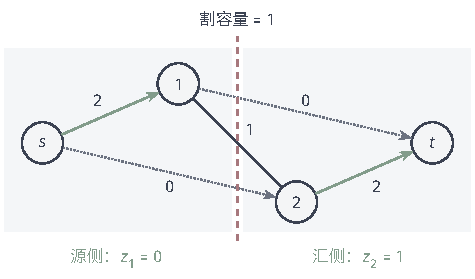
\includegraphics[width=80.405mm]{figures/09-probabilistic-graphical-models/02-inference/tikz/pgm-variational-cut/figure.pdf}
  \caption{两变量次模能量的$s$--$t$割网络。源侧编码为$0$，汇侧编码为$1$；实线终端边容量为$2$，点线终端边容量为$0$，中间无向边容量为$1$。虚线表示分开$\{s,1\}$和$\{2,t\}$的割，容量为$1$，对应配置$(0,1)$。}
  \label{fig:pgm-variational-cut}
\end{figure}

\subsubsection{多标签能量的局部优化}
\label{sec:pgm-variational-multilabel-cuts}

次模图割只解决二值问题。当每个变量有多个标签（不止0/1）时，一次割无法表达全部选择，常用的局部搜索是\emph{反复把多标签问题临时化成二元问题}：$\alpha$扩展每轮挑一个候选标签$\alpha$、让每个节点决定“保留现标签还是改成$\alpha$”（这一步在度量型代价下次模、可精确用图割解），逐轮尝试所有标签直到没有改进；$\alpha$-$\beta$交换则只允许当前标为$\alpha$或$\beta$的节点在这两个标签间重排。它们只保证局部最优，$\alpha$扩展在Potts能量下还有一个“至多两倍最优”的近似比保证。对多标签变量，一次$s$--$t$割只能表达两个选项。\term{$\alpha$扩展}（$\alpha$-expansion）固定当前标签$\ell_i$，让每个节点选择保留$\ell_i$或改为$\alpha$，把这一步化为二元问题。令动作变量$y_i=0$表示保留$\ell_i$、$y_i=1$表示改为$\alpha$，则一条边在四种动作下的代价为
\[
  \begin{array}{ccc}
      &y_j=0&y_j=1\\
    y_i=0&V_{i,j}(\ell_i,\ell_j)&V_{i,j}(\ell_i,\alpha)\\
    y_i=1&V_{i,j}(\alpha,\ell_j)&V_{i,j}(\alpha,\alpha)
  \end{array}.
\]
因此，能够使用上一小节的图割，取决于这张二元表是否次模。若成对项为$w_{i,j}d(k,l)$，$w_{i,j}\geq0$且$d$是标签上的度量，三角不等式给出
\[
  d(\ell_i,\ell_j)+d(\alpha,\alpha)
    \leq d(\ell_i,\alpha)+d(\alpha,\ell_j).
\]
所以每个扩展子问题次模，能精确求解。循环标签并只接受严格改善，有限状态下会停在对所有扩展动作都无法改进的配置，但未必是全局最优。

$\alpha$--$\beta$交换采用另一种二元动作：当前标为$\alpha$或$\beta$的节点是活跃节点，每个活跃节点独立选择$\alpha$或$\beta$，其他节点的标签保持固定。这不是强制两个节点互换标签；活跃节点可以共同改成同一标签。两个活跃节点之间的次模条件为
\[
  V_{i,j}(\alpha,\alpha)+V_{i,j}(\beta,\beta)
    \leq V_{i,j}(\alpha,\beta)+V_{i,j}(\beta,\alpha).
\]
例如，非负、对称且对角值为零的成对代价满足这一条件，即使它不满足标签间的三角不等式。只有一个端点活跃的边，在非活跃端标签固定后成为一元项，因此不会增加二元次模限制。交换由此可处理这类不能直接用于所有扩展动作的代价。

近似比保证还要固定原始能量的形式。对于
\[
  E(\bm\ell)=\sum_iD_i(\ell_i)
       +\sum_{(i,j)\in E}w_{i,j}\mathbb I[\ell_i\ne\ell_j],
  \qquad D_i(k)\geq0,\quad w_{i,j}\geq0,
\]
即非负一元项与非负边权的Potts能量，完全达到扩展局部最优的返回配置$\bm\ell_{\mathrm{return}}$满足经典保证$E(\bm\ell_{\mathrm{return}})\leq2E^\star$，其中$E^\star=\min_{\bm\ell}E(\bm\ell)$。这里要求对每个标签都已没有改善的扩展动作，提前停止并不能直接使用该保证。其他度量或不同停止状态需要相应的近似比分析；能量平移也会改变乘法比值，不能在任意移去常数后仍照用两倍界。更一般的扩展、交换与近似比结果参见Boykov等人\scite{pgm-variational-boykov2001}。

标签本身若有自然次序，还可能利用更强的代价结构。例如，标签为$0,\ldots,K-1$，成对代价为$w_{i,j}g(\ell_i-\ell_j)$、$w_{i,j}\geq0$，且$g$在允许的整数差值上满足$g(r+1)-2g(r)+g(r-1)\geq0$。这个二阶差分条件表示标签差每增加一单位所带来的增量代价不会下降，即离散凸性。在一元代价有限的这一设定下，可以把一个标签编码为一串有序阈值：标签为$k$，就表示它越过前$k$层阈值。多层图用这些阈值节点及保持次序的约束表示标签，在满足相应图表示条件时可一次精确求解。这条路线依赖有序标签和凸代价的结构，不能直接覆盖一般多标签能量\scite{pgm-variational-ishikawa2003}。

一般多标签或非次模能量仍可能需要其他松弛与搜索方法。二元变量的任意成对代价可写成常数、一次项和$z_iz_j$项之和；因为变量取布尔值而函数值取实数，这类目标称为二次伪布尔函数。某些相应松弛，例如具有持久性性质的图割松弛，可返回部分确定的$0/1$标签，其余节点标为未定。这里“确定”的保证是：至少存在一个全局最优配置，与所有已给出的标签相容；它不保证任意补全其余标签都最优。未定部分仍需继续求解、搜索或补全，并在原能量下评价最终配置\scite{pgm-variational-kolmogorov2007qpbo}。

\subsection{可行配置恢复与最优性诊断}

\label{sec:pgm-variational-tightness-rounding}

用松弛/对偶求得可计算上界，再通过取整或图割得到合法配置后，可用原始--对偶间隙评价该配置与最优值的距离。松弛值给出上界，已找到配置的真实得分给出下界；二者之差构成无需知道真值的次优性证书，间隙为零即证明全局最优。分数解在次模或树结构下可以无损取整，此时松弛是紧的。对于二元次模能量，共同阈值取整可以直接证明局部LP松弛是紧的。令$m_i=\mu_i(1)$。对任何局部一致的边表，$\Pr(Z_i\ne Z_j)\geq|m_i-m_j|$，因为$m_i-m_j=\mu_{i,j}(1,0)-\mu_{i,j}(0,1)$。非负$w_{i,j}$使松弛能量不小于
\[
  C+\sum_i[(1-m_i)D'_i(0)+m_iD'_i(1)]
       +\sum_{(i,j)}w_{i,j}|m_i-m_j|.
\]

令所有节点共用$U\sim\operatorname{Uniform}(0,1)$，取$z_i=\mathbb I[U<m_i]$，则节点均值为$m_i$，不同值概率恰为$|m_i-m_j|$。这个全局分布的期望能量等于上式，所以至少有一个阈值配置的能量不高于原LP解。用于LP最优解时，结合松弛下界便得到整数最优值等于LP最优值。因此LP存在整数最优解；存在平局时，若干整数最优解的分数混合也可能达到同一最优值。按排序后的$m_i$检查至多$d+1$个阈值区间即可寻找相应配置。

树图上的局部LP同样是紧的。局部一致表可以构造全局树分布，其期望得分不超过某个配置的得分，因此松弛最优值等于整数最优值，并存在整数最优解。树上的一般边缘仍可以是分数。含环图的紧性需要结合结构、势函数与参数判断，消息收敛本身只说明更新的状态。

对于一般LP分数解，可以逐点选择最大伪边缘、联合取整、局部搜索，或使用切平面和分支定界。逐点选择可能破坏变量之间的协调；存在硬约束时，还需检查恢复的配置是否可行，并在原目标下计算其得分。

对得分最大化，保留已找到的最好可行值$L=S(\widehat{\bm z})$及一个经验证的对偶上界$U$，则
\begin{equation}
  0\leq M-S(\widehat{\bm z})\leq U-S(\widehat{\bm z}).
  \label{eq:pgm-variational-gap}
\end{equation}
右侧是可计算的\term{原始--对偶间隙}（primal--dual gap），在此处比较整数可行解与松弛对偶证书。若还记录一个LP原始可行解$\bm\mu$的目标值$P=\langle\bm\theta,\bm\mu\rangle$，就能增加对求解过程的诊断，但要区分几个不同对象。对同一个LP及其对偶，有
\[
  U\geq U_{\mathrm{LP}}\geq M\geq L,
  \qquad P\leq U_{\mathrm{LP}}.
\]
其中$U$是对偶可行值，$U_{\mathrm{LP}}$是LP真正的最优值；$P$只是在当前分数可行点达到的值。由第一条链可知，$U-L$确实控制当前整数配置的次优损失。由第二条关系可知，$U-P\geq0$是可计算的LP求解差距，并且同时满足$0\leq U-U_{\mathrm{LP}}\leq U-P$与$0\leq U_{\mathrm{LP}}-P\leq U-P$。所以$U-P$小时，LP原始、对偶两侧的目标值都已接近LP最优值。

$P$与$L$之间却没有固定的大小关系。尚未充分优化的分数点可能比已经找到的合法配置得分还低，因此$P-L$不能无条件称为非负的“取整损失”。即使已经知道$P=U_{\mathrm{LP}}$，$P-L$也同时包含LP与整数问题的差别以及当前配置尚未最优的差别。更完整的关系为
\[
  U-L
    =(U-U_{\mathrm{LP}})
       +(U_{\mathrm{LP}}-M)+(M-L).
\]
三项依次是对偶尚未优化到LP最优值的差距、LP松弛间隙、当前配置相对整数最优值的次优损失，均非负。通常$U_{\mathrm{LP}}$和$M$并未知晓，后两项尤其不能仅凭当前$U,P,L$分别观测；记录三个当前值能提供证据，却不能自动完成这一分解。

对能量最小化，方向反过来：松弛或对偶提供下界，可行配置提供上界。在三角例中，逐点按平局选$0$得到得分$0$；把任一变量翻转便达到$2\beta$，但LP上界仍为$3\beta$。由于本例的整数真值与LP最优值都能独立算出，可以明确判断局部改进消除了当前配置的次优损失，却没有修复$\beta$的松弛间隙。再取三角例的均匀独立分布所诱导的局部表，得到LP原始可行值$P=3\beta/2$；与刚才的合法配置$L=2\beta$相比，$P-L=-\beta/2<0$，直接显示两者不具有固定顺序。

LP对偶的凸性支持全局求解，但求得$U_{\mathrm{LP}}$后，整数最优值仍可能更低。若一个合法配置达到对偶值，则配置与上界之间的间隙为零，可以立即形成全局最优证书。对于TRW消息算法，还需检查具体调度如何优化上界；目标的凸性与某种更新的单调性属于不同的论证。

MPE分解把计算分配给子问题。成对树上的一次最大和及回溯需$O(|E_T|k^2)$；多棵树可并行，但共享乘子的协调和通信仍在。显式局部LP有约$O(dk+mk^2)$个变量，其求解时间不只由变量数决定，还受求解器、约束和容差影响。图割属于多项式时间的特殊精确子问题，一次扩展只解一个二元动作，整体还要计入标签轮数。衡量可扩展性时，应同时报告单轮计算、存储、通信和达到所需诊断标准的轮数。

MPE近似需要另一套记录：原约束是否满足、可行配置得分是多少、对偶上界是多少，以及它们的差距。三角图的结论可同时列出：完全平均场的对数配分函数下界为$3.119162$，结构化固定点的同类下界为$3.178054$，精确$\log Z_\beta=3.258097$，Bethe固定点的对数配分函数近似为$3.295837$。MPE方面，最好可行得分为$2\log2=1.386294$，LP与该树分解的上界为$3\log2=2.079442$。前一组数值比较对数配分函数，后一组比较最大配置得分；它们需要分别展示对应的真值与界。

原始--对偶间隙直接控制当前配置相对于最优得分的损失。后验是否集中在该配置附近，以及各变量的边缘概率，还需由分布查询回答。间隙较大时，先用可计算的$U-P$检查LP是否还未求解充分，再尝试改进合法配置或加强一致性约束。对偶优化误差、松弛间隙和配置次优损失是不同来源；除非另有精确解或证书，不能声称已经把它们分别测出。可以根据现有上下界及改进结果，选择继续求解、加强松弛或接受已量化的总误差范围。配置推断的结果应同时包含合法配置及其得分证书。

\section{本章小结}

\label{sec:pgm-variational-summary}

本章以已知模型下的两类查询组织近似推断。对于后验分布，ELBO用反向KL连接近似分布与目标；平均场和结构化VI通过限制$q$的依赖，使期望和真实熵可计算。共轭消息、小批量更新与摊销映射分别减少局部期望计算、数据遍历和逐样本优化的成本，近似族误差则取决于所保留的结构。

局部自由能维护伪边缘，以局部一致性和熵近似替代全局分布计算。树上这些关系精确，推广到含环图后形成Bethe与Kikuchi近似；更大的区域保留更多联合约束，也增加表格和通信成本。EP以倾斜分布的矩修正站点，拉普拉斯法用峰附近曲率构造高斯。各方法的优化或固定点性质需要与实际概率查询的误差分别检查。

对于全部非证据变量的MPE，目标是最大配置得分。边缘多面体上的线性优化与这一查询等价，局部多面体松弛给出上界，对偶分解与TRW便于计算证书，二元次模等特殊结构可用图割直接返回整数最优解。配置结果通过可行性和原始--对偶间隙诊断，分布结果通过支持、相关性和预测诊断。含求和变量的边缘MAP还需保留其求和运算，另按对应查询求解。

\paragraph{扩展阅读}
Wainwright与Jordan系统联系了指数族、变分目标和图结构，可用于进一步理解边缘多面体与熵对偶。阅读时可围绕近似边缘、最优配置和配分函数分别比较目标、可行域及界的方向，并考察局部计算所保留的依赖\scite{pgm-wainwright2008}。

\chapter{基于采样的近似推断}
\label{chap:pgm-sampling}

第~\ref{chap:pgm-elimination}、\ref{chap:pgm-junction-tree}章的精确推断和第~\ref{chap:pgm-variational}章的变分近似，都用确定的数值或近似分布描述后验。采样推断不直接求出整个后验分布，而是从后验中抽取一批代表性随机样本：估计故障的后验概率时，统计样本中故障出现的比例；估计期望时，对样本上的函数值取平均。当中间因子过大、高维积分没有闭式解，或合适的变分分布族难以选定时，样本统计量通常较少依赖模型的具体解析形式。它的代价是答案带随机误差且通常只能近似；增加样本可以压低误差，同一批样本还能回答多个查询。

从后验采样通常并不比求后验更容易，因为实际往往只知道未归一化的联合权重$p(\bm{x},\bm{z})$，不知道归一化常数。本章讨论四种间接获得后验代表性样本的机制及其成立条件。直接从目标生成独立样本时，可用大数定律分析样本均值；目标难以直接采样时，重要性采样从提议分布生成候选，再用权重修正差异；高维下难以构造全局提议时，MCMC从当前状态作局部移动，靠满足条件的Markov链使长期访问比例逼近后验；观测随时间逐步到来时，序贯蒙特卡洛/粒子滤波递推样本与权重，并淘汰低质量样本。每种机制分别讨论估计量的极限条件、有限计算误差和诊断方法。

\section{采样推断的定义}
\label{sec:pgm-sampling-definition}

采样估计建立在一个共同事实上：如果存在一批独立且服从后验的样本，就可以用样本平均代替后验期望，并量化估计误差。后续各种采样器主要解决如何获得这样的样本。先设观测为$\bm{x}$，潜变量为$\bm{z}$，固定模型参数并省略其记号。把目标后验写为
\begin{equation}
  \begin{aligned}
    p(\bm{z}\mid\bm{x})&=\frac{\gamma(\bm{z})}{Z_{\bm{x}}},&
    \gamma(\bm{z})&=p(\bm{x},\bm{z}),\\
    Z_{\bm{x}}&=\int\gamma(\bm{z})\,\mathrm{d}\bm{z},&
    I_h&=\mathbb{E}_{p(\bm{z}\mid\bm{x})}[h(\bm{z})].
  \end{aligned}
  \label{eq:pgm-sampling-target}
\end{equation}
其中$0<Z_{\bm{x}}<\infty$，$h$是待求期望的实值函数。本章的积分也涵盖离散情形，此时改为求和，$p$表示概率质量而非密度。$\gamma$可以计算到一个与$\bm{z}$无关的正比例常数；这足以计算后验期望，却不足以确定原模型的证据$Z_{\bm{x}}$。估计证据时，必须知道$\gamma$的实际尺度。

若能直接从后验获得独立同分布的$\bm{z}_1,\ldots,\bm{z}_n$，就可以用函数值的样本均值估计$I_h$：
\begin{equation}
  \widehat I_{h,n}=\frac{1}{n}\sum_{i=1}^{n}h(\bm{z}_i).
  \label{eq:pgm-sampling-direct-estimator}
\end{equation}
选择$h(\bm{z})=\mathbb{I}\{\bm{z}\in B\}$，即事件$B$发生时取$1$、否则取$0$的指示函数，就得到后验事件概率的估计；选择某个分量或分量乘积，则得到均值或二阶矩。同一批样本可以用于多个查询，各查询的误差由相应的函数$h$决定。采样平均、方差缩减和Markov链长期平均的概率基础可参考\BookChapterRef{chap:random-sequences-and-processes}{卷2《数学准备：概率、因果与决策》的“随机序列与随机过程”章}。

独立样本的极限理论提供这一估计量的正确性依据。可积$h$使样本均值几乎必然收敛；方差$\sigma_h^2=\operatorname{Var}_p(h)$有限时，估计量还满足下列方差与极限关系：
\begin{equation}
  \begin{aligned}
    \mathbb{E}[\widehat I_{h,n}]&=I_h,&
    \operatorname{Var}(\widehat I_{h,n})&=\frac{\sigma_h^2}{n},\\
    \sqrt n(\widehat I_{h,n}-I_h)&\xrightarrow{\mathrm{d}}
      \mathcal{N}(0,\sigma_h^2).
  \end{aligned}
  \label{eq:pgm-sampling-iid-clt}
\end{equation}
\term{蒙特卡洛标准误}（Monte Carlo standard error, MCSE）衡量重复运行估计过程时答案的波动，即再独立抽取同样多的一批样本时平均答案的变动幅度。独立样本下可用$s_h/\sqrt n$估计，其中$s_h^2$是$h(\bm z_i)$的样本方差。它与后验标准差有明确区别：后者描述模型本身固有的不确定性（故障是否可能发生），不随样本增多而消失；MCSE描述有限采样带来的计算波动（对该概率估计的偏差程度），随$n$增大趋于零。


\begin{example}[报警后的故障概率]
  \label{ex:pgm-sampling-device}
  沿用人工构造的设备模型$F\to H\to A\leftarrow S$：$F$表示故障，$H$表示过热，$A$表示报警，$S$表示传感器失灵。根节点$F,S$独立，且
  \[
    \begin{aligned}
      p(F=1)&=0.1,&p(S=1)&=0.05,\\
      p(H=1\mid F=1)&=0.8,&
      p(H=1\mid F=0)&=0.1.
    \end{aligned}
  \]
  报警条件表仍与前面的精确推断相同：
  \[
    \begin{array}{ccccc}
      (h,s)&(0,0)&(1,0)&(0,1)&(1,1)\\
      p(A=1\mid h,s)&0.01&0.9&0.7&0.99
    \end{array}
  \]
  边缘化故障得到$p(H=1)=0.17$，从而
  \[
    \begin{aligned}
      p(A=1\mid H=0)&=0.95\times0.01+0.05\times0.7=0.0445,\\
      p(A=1\mid H=1)&=0.95\times0.9+0.05\times0.99=0.9045,\\
      p(A=1)&=0.83\times0.0445+0.17\times0.9045=0.1907,\\
      p(F=1,A=1)&=0.1(0.2\times0.0445+0.8\times0.9045)=0.07325.
    \end{aligned}
  \]
  因此精确答案为$p(F=1\mid A=1)=0.07325/0.1907\approx0.384111$。若能够取得$10000$个独立后验样本，故障比例的理论标准误约为$\sqrt{0.384111(1-0.384111)/10000}=0.004864$。这个小模型的精确答案用于校验采样计算，不是实际设备数据。
\end{example}

改变样本生成机制后，误差分析也要随之改变。重要性样本由提议生成，估计方差取决于加权函数；一条Markov链上的状态通常相关，样本均值的方差需要计入协方差；重采样粒子还可能共享祖先。后文分别建立这些机制下的正确性条件，再分析相应的计算误差。普通蒙特卡洛误差与方差缩减的系统论述见Owen\scite{pgm-sampling-owen2013}。

\section{独立蒙特卡洛方法}
\label{sec:pgm-sampling-independent}

这一节讲独立蒙特卡洛的三种递进办法：能直接按目标生成时直接采样；直接采样困难但能找到一个“罩住”目标的简单分布时，用拒绝采样筛选；连罩住都困难时，保留所有候选、改用连续权重修正，即重要性采样。三者每次都使用新的独立随机输入，候选彼此独立，但自归一化权重共用一个随机分母，估计量的分析还需考虑这一比值结构。

\subsection{直接采样、祖先采样与拒绝采样}
\label{sec:pgm-sampling-direct-rejection}

当目标分布本身带有容易操作的生成规则（例如有向图的局部条件分布）时，可以按变量之间的依赖顺序把一个完整样本“逐步抽出来”，无需知道难算的归一化常数。每次生成完整记录时使用新的独立随机输入，得到的记录之间才具有独立性。

在有向无环图上，\term{祖先采样}（ancestral sampling）按拓扑顺序逐个生成节点，使每个节点采样时都已知道其父节点的取值。若一次生成$\bm{x}$时，第$i$个节点使用$p(x_i\mid\bm{x}_{\operatorname{pa}(i)})$，则整次生成的概率恰为这些条件概率之积，也就是图模型的联合分布。样本内部的各节点通常不独立，独立的是从头运行得到的不同完整样本。一次生成的成本包括拓扑遍历和所有局部条件分布的采样成本；后者取决于各条件分布的实现。

祖先采样很容易抽到联合分布，但我们真正想要的是给定证据（如$A=1$）后的后验。一个朴素办法是：照常按先验抽完整样本，然后只保留恰好符合证据的样本、丢弃其余。在设备模型上，若按先验生成$F,S,H$后直接把$A$强行设为$1$，保留下来的故障比例仍是先验的$0.1$，并不是后验；只有连同$A$一起按模型生成、再仅保留$A=1$的样本，所保留记录才服从后验，故障概率为$0.384111$。这种“先从简单分布生成候选、再按某个规则决定去留”的做法就是\term{拒绝采样}（rejection sampling）的特例。

拒绝采样的一般设定是：找一个容易采样的提议分布$q$，并让它的密度在每一处都不低于目标密度（允许差一个常数倍），候选落在目标密度相对越高的位置就越可能被接受、越低则越可能被拒绝。设$q(\bm{z})$为提议密度，已知常数$c<\infty$使$\gamma(\bm{z})\leq c q(\bm{z})$在整个目标支撑集上成立。独立生成$\bm{z}\sim q$和$u\sim\operatorname{Uniform}(0,1)$，当$u\leq\gamma(\bm{z})/[c q(\bm{z})]$时接受。对任意可测集合$B$，
\begin{equation}
  \begin{aligned}
    \mathbb{P}(\bm{z}\in B,\text{接受})
      &=\int_B q(\bm{z})\frac{\gamma(\bm{z})}{c q(\bm{z})}
        \,\mathrm{d}\bm{z}
        =\frac{1}{c}\int_B\gamma(\bm{z})\,\mathrm{d}\bm{z},\\
    \mathbb{P}(\text{接受})&=\frac{Z_{\bm{x}}}{c}.
  \end{aligned}
  \label{eq:pgm-sampling-rejection}
\end{equation}
相除便得到$\mathbb{P}(\bm{z}\in B\mid\text{接受})=\int_B p(\bm{z}\mid\bm{x})\,\mathrm{d}\bm{z}$。因此按固定规则独立重复试验，直到得到指定数量的接受样本，会产生独立同分布的目标样本。每个接受样本平均需要$c/Z_{\bm{x}}$次提议。这一结论依赖全局包络条件。只检查已生成的位置，无法保证未访问区域也满足相同的接受规则。

在报警例子中，匹配证据的接受率为$0.1907$，平均约$5.244$次联合采样得到一个后验样本。若有多个稀有离散证据，联合匹配概率可能很小；连续证据的精确等值事件通常概率为零，需要使用密度条件化等其他采样构造。高维包络也容易变松：若归一化目标和提议分别按坐标分解，每维包络常数为$m>1$，乘积包络的接受率便是$m^{-d}$。后验越集中而提议越分散，越多计算会用在最终丢弃的候选上。

\subsection{重要性采样}
\label{sec:pgm-sampling-importance}

拒绝采样的最大问题是大量候选会被白白丢弃，尤其当证据稀有、维度很高时接受率极低。换个角度：与其把不太符合目标的候选直接扔掉，不如全都保留，但让每个候选对最终估计的“话语权”按它与目标的吻合程度加权——吻合得好的权重大、吻合得差的权重小。\term{重要性采样}（importance sampling, IS）正是这样做的：从易采样的$q$生成候选，并以目标与提议的密度比修正抽样频率。这要求$p\ll q$，即$q$必须覆盖目标的所有正概率区域（否则目标在那些区域的质量永远采不到、也无从修正）；连续情形按测度理解，零测集上的密度取值不影响结论。

如果目标密度已归一化，令$r(\bm{z})=p(\bm{z}\mid\bm{x})/q(\bm{z})$，便有
\begin{equation}
  \begin{aligned}
    I_h&=\int h(\bm{z})r(\bm{z})q(\bm{z})\,\mathrm{d}\bm{z},\\
    \widehat I_{h,n}^{\mathrm{IS}}
      &=\frac{1}{n}\sum_{i=1}^{n}r(\bm{z}_i)h(\bm{z}_i).
  \end{aligned}
  \label{eq:pgm-sampling-is}
\end{equation}
只要$\mathbb{E}_p|h|<\infty$，这个估计无偏且一致；有限方差还要求$\mathbb{E}_q[r^2h^2]<\infty$。目标区域若只被$q$赋予很小概率，偶尔出现的巨大权重会主导结果。支持覆盖保证目标区域有机会被提议访问，加权矩条件进一步控制罕见访问带来的波动。

图模型往往只提供$\gamma$。令$w_i=\gamma(\bm{z}_i)/q(\bm{z}_i)$，同时估计分子积分和归一化常数，得到\term{自归一化重要性采样}（self-normalized importance sampling, SNIS）：
\begin{equation}
  \begin{aligned}
    \widehat Z_{\bm{x}}&=\frac{1}{n}\sum_{i=1}^{n}w_i,&
    \bar w_i&=\frac{w_i}{\sum_{j=1}^{n}w_j},\\
    \widehat I_{h,n}^{\mathrm{SNIS}}
      &=\frac{\frac{1}{n}\sum_i w_i h(\bm{z}_i)}
              {\frac{1}{n}\sum_i w_i}
       =\sum_i\bar w_i h(\bm{z}_i).
  \end{aligned}
  \label{eq:pgm-sampling-snis}
\end{equation}
要求本次权重和非零。$\widehat Z_{\bm{x}}$无偏，但两个无偏估计的比值通常有偏，因为随机分母不能移到期望之外。在支撑集覆盖、$0<\mathbb{E}_q w=Z_{\bm{x}}<\infty$和$\mathbb{E}_q|wh|<\infty$时，分子、分母分别由大数定律收敛，故比值仍然一致。因此，比值的有限样本偏差与样本数增长后的渐近一致性可以同时成立。

设备例子可以令$q(f,h,s)=p(f)p(s)p(h\mid f)$，不抽取已知的$A$，而令$w(f,h,s)=p(A=1\mid h,s)$。这称为\term{似然加权}（likelihood weighting）：证据通过似然而非硬性筛选影响候选。图~\ref{fig:pgm-sampling-importance}比较先验与报警后的$(H,S)$分布。先验最常生成“既不过热也未失灵”，但这一状态很难解释报警；乘上似然以后，它只占约$4.13\%$的后验质量。

\begin{figure}[!t]
  \centering
  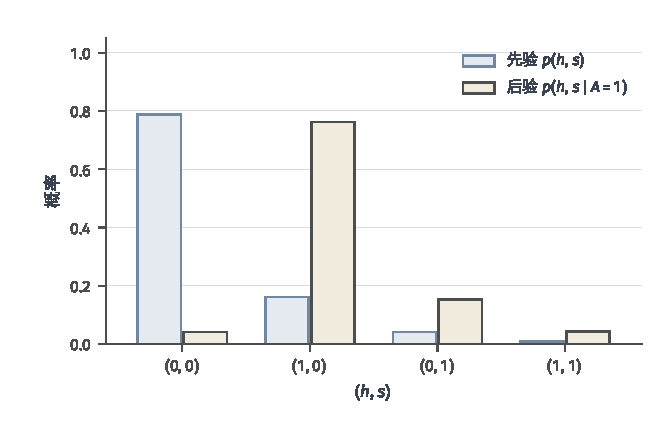
\includegraphics[width=105.412mm]{figures/09-probabilistic-graphical-models/02-inference/matplotlib/pgm-sampling-importance/figure.pdf}
  \caption{人工设备模型中$(H,S)$的先验与给定$A=1$后的后验。横轴每组的两位数依次为$h,s$；淡蓝柱表示先验，淡黄色柱表示后验。权重改变已有候选的贡献；未被抽到的类别仍需依靠后续生成访问。}
  \label{fig:pgm-sampling-importance}
\end{figure}

表~\ref{tab:pgm-sampling-weight-example}用四个可能的独立先验样本展示似然加权。直接计数的故障比例为$1/4$，加权比例为$0.9/(0.01+0.9+0.9+0.7)\approx0.358566$。权重按目标修正了候选贡献，但四次抽样仍有明显的有限样本波动，所得比例与精确后验不同。

\begin{table}[!t]
  \centering
  \begin{tabular}{ccccc}
    \toprule
    样本$i$ & $(f_i,h_i,s_i)$ & $w_i$ & $\mathbb{I}\{f_i=1\}$ & $w_i\mathbb{I}\{f_i=1\}$\\
    \midrule
    1 & $(0,0,0)$ & $0.01$ & $0$ & $0$\\
    2 & $(1,1,0)$ & $0.90$ & $1$ & $0.90$\\
    3 & $(0,1,0)$ & $0.90$ & $0$ & $0$\\
    4 & $(0,0,1)$ & $0.70$ & $0$ & $0$\\
    \bottomrule
  \end{tabular}
  \caption{似然加权的四样本教学计算。分母是全部权重之和，分子仅累加故障样本的权重。}
  \label{tab:pgm-sampling-weight-example}
\end{table}

提议的尾部决定极端权重出现的频率。即使提议很好地匹配后验峰附近，尾部事件估计仍需要足够的尾部覆盖。以一维标准正态目标$p=\mathcal{N}(0,1)$和$q=\mathcal{N}(0,s^2)$为例，其中$s>0$。二者的支撑集相同，但这只保证每个目标区域都有机会被访问。要判断权重的波动是否具有有限二阶矩，需要计算
\[
  \mathbb{E}_q[r^2]
    =\int \left(\frac{p(z)}{q(z)}\right)^2q(z)\,\mathrm{d}z
    =\int\frac{p(z)^2}{q(z)}\,\mathrm{d}z.
\]
将两个高斯密度代入，被积函数除去与$z$无关的正常数以后为
\[
  \frac{p(z)^2}{q(z)}
    \ \propto\ \exp\left[\left(-1+\frac{1}{2s^2}\right)z^2\right].
\]
当二次项系数$-1+1/(2s^2)$为负时，被积函数在两端都按高斯速度衰减，积分有限。系数为零时，被积函数是正常数，在整条实线上积分仍然发散；系数为正时，它随$|z|$增长，积分也发散。因此$\mathbb{E}_q r^2$只有在$s^2>1/2$时才有限。这是权重本身的二阶矩判据；具体查询的IS方差还要检查前述$\mathbb{E}_q[r^2h^2]$，不能仅凭权重二阶矩替任意$h$作保证。

提议过窄时，算法可以满足一致性的条件，却没有通常所需的有限权重二阶矩；重复运行中偶发的大权重会破坏熟悉的误差估计。如何构造尾部足够宽、同时不过度浪费样本的提议，是重要性采样的主要计算问题；相关分析可参见Owen教材的第9章\scite{pgm-sampling-owen2013}

\subsection{方差缩减}
\label{sec:pgm-sampling-variance-reduction}

增加样本数$n$总能压低误差，但代价是采更多样本。蒙特卡洛里还有另一类不增加样本、而是巧妙利用解析计算来减小单次随机贡献波动的办法，统称为方差缩减。这里介绍两种最常用的：一种用一个期望已知的相关量去抵消共同波动（控制变量），另一种把原本要靠抽样的部分改用精确积分算掉（Rao–Blackwell化）。

除了增加独立样本数，还可以通过减小单次随机贡献的方差来降低MCSE。设一次独立抽样原本给出随机贡献$Y$，待求量为$\mathbb{E}Y$。若能同时计算另一个随机量$G$，且其期望$\mu_G$已知，就可以用$G-\mu_G$记录这次抽样相对已知均值的偏离。对预先固定的系数$a$，以$Y-a(G-\mu_G)$替换$Y$不会改变期望，因为被减去部分的期望为零。这就是控制变量（control variates）的作用：利用已知期望修正样本函数。在$Y,G$均有有限方差时，
\[
  \operatorname{Var}\bigl(Y-a(G-\mu_G)\bigr)
    =\operatorname{Var}(Y)-2a\operatorname{Cov}(Y,G)
       +a^2\operatorname{Var}(G).
\]
若$\operatorname{Var}(G)>0$，使该二次式最小的系数为
\[
  a=\frac{\operatorname{Cov}(Y,G)}{\operatorname{Var}(G)}.
\]
代入这个系数后，方差的减少量为$\operatorname{Cov}(Y,G)^2/\operatorname{Var}(G)$。因此收益来自两种贡献之间可被抵消的共同波动，并非任意选择控制变量和系数都会减小方差。若总体协方差未知，可以用独立的先导样本估计$a$，再在正式抽样中固定该系数；若用同一批样本估计$a$并回代，系数与样本贡献会相互依赖，需另查偏差，不能直接继承固定系数时的无偏结论。

另一种波动来自完整记录中并非必须抽取的变量。若保留随机量$U$以后，仍能解析计算其余随机性下的条件平均，就可以把$Y$替换为$\widetilde Y=\mathbb{E}[Y\mid U]$。这种Rao--Blackwell化（Rao--Blackwellization）将部分抽样替换为条件积分。在图模型中，局部消元可以解析消去部分节点，仅对保留变量采样。条件积分必须使用原联合分布在给定$U$后的条件分布；这样的相容条件期望才保持原均值。由迭代期望和全方差关系，有限二阶矩下有
\[
  \begin{aligned}
    \mathbb{E}\widetilde Y&=\mathbb{E}Y,\\
    \operatorname{Var}(Y)
      &=\operatorname{Var}(\widetilde Y)
        +\mathbb{E}\bigl[\operatorname{Var}(Y\mid U)\bigr]
       \geq\operatorname{Var}(\widetilde Y).
  \end{aligned}
\]
被消去的是给定$U$以后仍会发生的抽样波动，右侧的条件方差项正好度量这部分波动。在相同独立抽样次数下，样本均值的方差也随之不增。

若目标是设备的先验报警概率，可以抽取完整$(F,H,S,A)$并平均$\mathbb{I}\{A=1\}$，也可以只抽取$F$，把其余节点解析消去。这里原贡献是$Y=\mathbb{I}\{A=1\}$，保留变量是$U=F$，所以替换后的贡献为$\mathbb{E}[Y\mid F]=p(A=1\mid F)$。它按原模型的$p(H,S,A\mid F)$积分，而非另换一个容易计算的条件分布。当$F=0$时，这个条件报警概率为$0.1305$；当$F=1$时为$0.7325$。两者均值都是$0.1907$，但前者单样本方差为$0.1907(1-0.1907)=0.15433351$，后者为$0.1\times0.9(0.7325-0.1305)^2=0.03261636$。解析计算减少了相同独立抽样次数下的方差；是否节约总时间，还要比较条件积分的成本。

方差缩减需要作用于完整估计量。SNIS的分子贡献为$wh$，分母贡献为$w$，因此要按提议的条件分布同时积分这两个量，保持权重与函数的相容关系。具体地，把提议下的变量分为$(U,V)$，仅抽取$U_i\sim q_U$，再计算
\[
  \begin{aligned}
    A(U)&=\mathbb{E}_q[w(U,V)h(U,V)\mid U],\\
    B(U)&=\mathbb{E}_q[w(U,V)\mid U],\\
    \widehat I_{h,n}^{\mathrm{RB\text{-}SNIS}}
      &=\frac{\sum_{i=1}^{n}A(U_i)}{\sum_{i=1}^{n}B(U_i)}.
  \end{aligned}
\]
这两个条件平均都使用$q(V\mid U)$，所以分子与分母的期望仍分别为$Z_{\bm{x}}I_h$和$Z_{\bm{x}}$。权重和非零且原来的可积性条件成立时，比值仍然一致；它通常仍有有限样本偏差。在对应二阶矩存在时，分子和分母各自的方差不增，仍不能单独推出其比值在每个有限样本量下也有更小方差，还须分析两者的共同波动。

为观察这一共同波动，可以在分析中把两者组合成$A(U)-I_hB(U)=\mathbb{E}_q[w(h-I_h)\mid U]$，实现上述估计时仍只需分别计算$A$和$B$。后文的比值展开会说明，$w(h-I_h)$正是原SNIS一阶误差的单样本贡献。因此在对应中心极限定理的矩条件下，对这个贡献取条件平均会使渐近方差不增；这个结论针对样本量增长时的一阶误差，不是所有有限样本比值的方差排序。MCMC均值的渐近方差还包括时间相关性，单次函数方差减小后，需要继续检查自相关如何变化。

\section{Markov链蒙特卡洛}
\label{sec:pgm-sampling-mcmc}

前面的独立方法（包括重要性采样）都隐含一个要求：能一次性构造一个在整个高维空间都覆盖良好的提议分布。但在高维、强相关的后验中，找到这样的全局提议往往和直接求后验一样难。换个思路：不必一次想清楚要跳到哪里，只要规定“站在当前位置时，下一步往附近怎么走”即可——用一个只依赖当前状态的局部规则反复走，走出一条状态序列；只要这个局部规则设计得当，长期来看序列造访各个状态的频率就会正比于其后验概率。\term{Markov链蒙特卡洛}（Markov chain Monte Carlo, MCMC）就是通过这样的局部转移形成\emph{相关}样本序列，再用长期平均近似目标期望。注意这些样本不再独立（相邻状态很接近），所以误差分析与独立样本不同；其正确性依赖两件事：转移规则保持目标分布，以及链长期运行能够充分访问目标的各个区域。

\subsection{Markov转移与目标分布}
\label{sec:pgm-sampling-markov-kernel}

局部转移规则必须保持目标分布不变。令$\bm z^{(k)}$为第$k$次迭代状态，$K(\bm z,B)$表示从当前状态转移到集合$B$的概率。若某一步的状态分布已经等于目标后验，再用该规则更新一步后仍应得到目标后验；否则这条链不能把目标分布作为稳定状态。把每个起点的后验权重与它转移到$B$的概率相乘并积分，就得到下一状态落入$B$的概率。要求它仍等于目标对$B$分配的概率，即
\begin{equation}
  \int p(\bm{z}\mid\bm{x})K(\bm{z},B)\,\mathrm{d}\bm{z}
    =\int_B p(\bm{z}'\mid\bm{x})\,\mathrm{d}\bm{z}'.
  \label{eq:pgm-sampling-invariance}
\end{equation}
满足此式时，$p$称为\term{平稳分布}（stationary distribution）：若当前状态已服从$p$，再转移一步仍服从$p$。该条件描述状态分布，单条轨迹仍可移动。但保持目标并不保证能从任意初值走到目标。例如，每一步都停在原地的规则保持任何分布，却只会反复输出同一个初值；它无法估计未访问区域的概率。从指定初值到达目标还需可达性等条件。

使往返概率流相等的细致平衡，是上述不变性的一个充分条件。在当前后验与转移核上，它写为
\begin{equation}
  p(\mathrm{d}\bm{z}\mid\bm{x})K(\bm{z},\mathrm{d}\bm{z}')
    =p(\mathrm{d}\bm{z}'\mid\bm{x})K(\bm{z}',\mathrm{d}\bm{z}).
  \label{eq:pgm-sampling-detailed-balance}
\end{equation}
测度记号包含拒绝后原地停留的点质量。对一端积分即可得到不变性。
顺次组合多个保持$p$的核仍保持$p$，但组合后的核未必可逆。

不变性之外，时间平均还需要链能够访问并返回目标的相关区域。对有限状态空间，不可约表示任意两个状态之间都能经有限步以正概率到达；这排除了被隔开的封闭状态类。有限不可约链的时间平均可收敛，但逐步状态分布收敛还需要非周期性，也就是返回时刻没有共同的、严格大于一的周期约束。例如，链确定地在$0$和$1$之间轮换，时间平均中两者的比例都趋于$1/2$；若从$0$启动，第$k$步的位置却由奇偶性决定，逐步状态分布不会趋于均匀分布。这个例子区分了长期访问比例与某一步位置的分布。

一般状态空间中，单点的目标概率可能为零，因而要把可达和返回的要求放在具有正目标概率的集合上。后文使用正Harris常返性：在所声明的状态类内，从每个起点出发，都以概率一反复访问每个具有正目标概率的可测集合，并且该类具有可归一化为概率分布的平稳测度。它把“能进入相关区域”加强为足以支持长期平均的返回性质。结合查询函数对目标分布可积，便可在这个状态类内讨论时间平均的几乎必然收敛；状态类之外的任意初值不自动包含在保证中。后文据此构造后验更新，再分别说明误差分析所用的起点条件，检查有限预算中的探索。

采样核的设计先检验不变性、可达性与返回条件，再分析探索速度。\term{混合}（mixing）描述链摆脱初值并访问目标分布的快慢。两个高概率区域之间存在低概率通道时，局部移动可能很难跨过它，即使渐近平均正确，有限预算中的估计仍可能偏向已访问的区域。

\subsection{Metropolis--Hastings方法}
\label{sec:pgm-sampling-mh}

现在给出最通用的MCMC规则Metropolis–Hastings（MH）：提议分布可以随便选，再用接受率校正它，使整条链保持目标分布，且不需要归一化常数。给定当前位置$\bm{z}$，设易采样提议为$q(\bm{z}'\mid\bm{z})$。若直接接受，往返概率流一般不相等。\term{Metropolis--Hastings方法}（Metropolis--Hastings, MH）通过位置相关的接受率，让实际往返流量都等于提议流量中较小的一方：
\begin{equation}
  \alpha(\bm{z},\bm{z}')
    =\min\left\{1,\,
      \frac{\gamma(\bm{z}')q(\bm{z}\mid\bm{z}')}
           {\gamma(\bm{z})q(\bm{z}'\mid\bm{z})}\right\}.
  \label{eq:pgm-sampling-mh-acceptance}
\end{equation}
从$\gamma(\bm{z})>0$的有效状态开始，提议到目标质量为零或无法反向提议的状态时拒绝；未实际提议到的零分母情形不参与该比值的计算。对两个不同状态，接受后的概率流为
\[
  \begin{aligned}
    &p(\bm{z}\mid\bm{x})q(\bm{z}'\mid\bm{z})\alpha(\bm{z},\bm{z}')\\
    &\qquad=\frac{\min\{\gamma(\bm{z})q(\bm{z}'\mid\bm{z}),
                    \gamma(\bm{z}')q(\bm{z}\mid\bm{z}')\}}
         {Z_{\bm{x}}}.
  \end{aligned}
\]
右侧交换$\bm{z},\bm{z}'$后不变；拒绝产生的原地停留也满足细致平衡。因此MH保持目标分布，并且不需要知道$Z_{\bm{x}}$。

MH每次先抽取提议，再用独立均匀数决定接受。接受时记录$\bm{z}'$，拒绝时继续记录$\bm{z}$。重复记录保留链在各状态停留的时间，删除这些记录会改变访问比例。独立拒绝采样以筛选得到目标独立样本，MH则以包含停留的相关轨迹保持目标。

随机游走提议常写作$\bm{z}'=\bm{z}+\epsilon\bm{\eta}$，其中$\bm{\eta}\sim\mathcal{N}(\bm{0},\bm{C})$，$\epsilon$为尺度，$\bm{C}$为给定正定矩阵。提议对称时，接受率只剩目标密度比。对标准正态目标，从$z=0$提议到$z'=2$的接受率是$\exp(-2)\approx0.1353$，反向提议则总被接受。尺度过小时，接受率虽高，每步位移却很小；尺度过大时，候选常落入低密度区域，链又因拒绝而停留。

维度会加重这一矛盾。对$p(\bm{z})\propto\exp(-\lVert\bm{z}\rVert_2^2/2)$，记$U(\bm{z})=-\log p(\bm{z})$并忽略其中与位置无关的常数。这个负对数密度也称势能：目标密度越小，势能越高。对称提议的接受率于是为$\min\{1,\exp[-\Delta U]\}$，其中$\Delta U=U(\bm{z}')-U(\bm{z})$。为看清维度的作用，这里固定每个坐标的噪声方差为$1$，取各向同性的$\bm{\eta}\sim\mathcal{N}(\bm 0,\bm I_d)$。势能变化为
\[
  \frac{\lVert\bm{z}+\epsilon\bm{\eta}\rVert_2^2
             -\lVert\bm{z}\rVert_2^2}{2}
    =\epsilon\bm{z}^{\top}\bm{\eta}
       +\frac{\epsilon^2}{2}\lVert\bm{\eta}\rVert_2^2.
\]
在这个固定噪声方差的设定下，$\mathbb{E}\lVert\bm{\eta}\rVert_2^2=d$，且其方差为$2d$，所以噪声平方范数通常与$d$同阶。若当前位置已服从标准高斯目标，且提议噪声独立，则交叉项$\epsilon\bm{z}^{\top}\bm{\eta}$的均值为零、方差为$\epsilon^2d$；正的二次项均值则为$\epsilon^2d/2$。固定$\epsilon>0$并增大$d$时，后者的增长快于交叉项的典型波动，使提议的势能差通常很大，接受率随之降低。将$\epsilon$缩小到与$d^{-1/2}$同阶可以控制这两个项的尺度，但每个坐标的提议位移也同时缩小，探索需要更多步。这些关系解释了固定尺度会让接受困难、缩小尺度又减缓单坐标探索的矛盾；它们针对当前高斯目标和固定坐标噪声方差的例子。一般后验的合适尺度还取决于其几何结构。

\term{独立提议}（independence proposal）取$q(\bm{z}'\mid\bm{z})=q(\bm{z}')$。候选不依赖当前位置，但接受后的链仍然相关。它能一次跨越很远的区域；为判断这种远距离候选能否被接受，把独立提议代入MH比值，得到
\[
  \frac{\gamma(\bm{z}')q(\bm{z})}
       {\gamma(\bm{z})q(\bm{z}')}
    =\frac{\gamma(\bm{z}')/q(\bm{z}')}
            {\gamma(\bm{z})/q(\bm{z})}
    =\frac{w(\bm{z}')}{w(\bm{z})},\qquad w=\frac{\gamma}{q}.
\]
因此接受率变成$\min\{1,w(\bm{z}')/w(\bm{z})\}$。一旦当前位置落入$q$严重低估的目标区域，当前权重$w(\bm{z})$就会很大；而从$q$生成的通常候选可能具有小得多的权重，使接受率很低。反复拒绝便使链在这一位置停留很久，尽管候选本身每次独立生成。独立提议依赖全局覆盖，随机游走依赖局部尺度。比较两者需要同时检查移动距离、停留和所需查询的估计误差。

\subsection{Gibbs采样}
\label{sec:pgm-sampling-gibbs}

MH需要自己设计提议和接受率。对图模型有一个更省事的特例：一次只更新一个变量，而该变量“在其余所有变量给定时的条件分布”往往因为Markov毯而形式简单、可以直接抽样——此时连接受率都是$1$，提议即被无条件接受。这就是Gibbs采样。图模型常允许直接计算一个变量在其余变量给定时的条件分布。\term{Gibbs采样}（Gibbs sampling）固定其余坐标，仅从待更新坐标的\term{满条件分布}（full conditional distribution）重新抽样；“满”表示已经给定其他全部未知变量及证据。记$\bm{z}_{-j}$为去掉第$j$个坐标后的向量，则单坐标更新使用$p(z_j\mid\bm{z}_{-j},\bm{x})$。顺序扫描时，一轮中已更新的坐标使用新值，尚未更新的坐标使用旧值。

满条件抽样可以看成接受率为一的MH更新。把固定$\bm{z}_{-j}$时的提议写成$q(z'_j\mid z_j,\bm{z}_{-j})=p(z'_j\mid\bm{z}_{-j},\bm{x})$，MH比值为
\begin{equation}
  \frac{p(z'_j,\bm{z}_{-j}\mid\bm{x})p(z_j\mid\bm{z}_{-j},\bm{x})}
       {p(z_j,\bm{z}_{-j}\mid\bm{x})p(z'_j\mid\bm{z}_{-j},\bm{x})}
    =1.
  \label{eq:pgm-sampling-gibbs-acceptance}
\end{equation}
等式来自联合分布的条件分解，并要求涉及的条件分布定义良好。每个更新核都保持后验，故依次组合一整轮也保持后验。若用近似满条件作提议，就不再有这个抵消；必须加入相应MH校正，或另行证明近似更新的偏差与收敛性质。随机扫描每次选一个坐标与确定性顺序扫描都可构造正确核，但整轮顺序扫描一般不满足细致平衡。

满条件虽然写成“给定所有其他变量”，实际计算通常只涉及邻近因子。有向图中，一个节点的\term{Markov毯}（Markov blanket）由父节点、子节点以及子节点的其他父节点组成；给定这些变量以后，其余节点不再改变该节点的条件分布。用$\operatorname{ch}(j)$记子节点集合，含有$z_j$的局部因子给出
\[
  p(z_j\mid\bm{z}_{-j},\bm{x})
    \ \propto\ p(z_j\mid\text{父节点})
       \prod_{\ell\in\operatorname{ch}(j)}
          p(v_\ell\mid\text{其父节点}),
\]
其中$v_\ell$表示子节点的当前取值，证据节点使用已观测值。无向图只需相乘所有包含该节点的势函数，再对候选$z_j$归一化。局部因子减少了单步计算范围，样本的跨迭代相关性仍取决于整个更新过程。

在设备后验$p(f,h,s\mid A=1)$上，更新$F$时只需$H$；若$H=1$，
\[
  p(F=1\mid H=1,A=1,S)
    =\frac{0.1\times0.8}{0.1\times0.8+0.9\times0.1}
    =\frac{8}{17}.
\]
更新$H$时则需$F,S,A$；若$F=1,S=0,A=1$，取$H=1$和$H=0$的未归一化概率分别为$0.8\times0.9=0.72$和$0.2\times0.01=0.002$，故前者的满条件概率是$0.72/0.722\approx0.997230$。更新$S$时，若$H=0,A=1$，则
\[
  p(S=1\mid H=0,A=1,F)
    =\frac{0.05\times0.7}{0.05\times0.7+0.95\times0.01}
    \approx0.786517.
\]
这三步展示了证据如何通过局部更新传播，而无须每次重新消去整张图。对有$K$个取值的节点，一次朴素更新需评估$K$组相关因子；块越大，联合条件分布的构造和抽样成本通常越高。

满条件更新的接受率为一，但强相关仍会限制每步移动。以零均值、相关系数$\rho\in(-1,1)$、边缘方差为$1$的二维高斯为例，其协方差矩阵为$\bigl(\begin{smallmatrix}1&\rho\\\rho&1\end{smallmatrix}\bigr)$。把联合密度中含$z_1$的二次项配方，有
\[
  z_1^2-2\rho z_1z_2+z_2^2
    =(z_1-\rho z_2)^2+(1-\rho^2)z_2^2.
\]
联合密度的指数是上述二次型乘以$-1/[2(1-\rho^2)]$。固定$z_2$后，配方后的第二项不影响$z_1$的条件密度，剩余部分正是均值$\rho z_2$、方差$1-\rho^2$的高斯密度，所以$z_1\mid z_2\sim\mathcal{N}(\rho z_2,1-\rho^2)$；交换两个坐标便得到$z_2\mid z_1$的相应表达式。满条件方差均为$1-\rho^2$，因此当$\rho$接近$1$时，给定一个坐标后另一个只能小幅移动。顺序更新满足
\[
  \begin{aligned}
    z_1^{(k+1)}&=\rho z_2^{(k)}+\sqrt{1-\rho^2}\epsilon_1,\\
    z_2^{(k+1)}&=\rho z_1^{(k+1)}+\sqrt{1-\rho^2}\epsilon_2,
  \end{aligned}
\]
其中每轮使用两个新的独立标准正态噪声$\epsilon_1,\epsilon_2$，它们也独立于此前的状态。把第一式代入第二式，得到
\[
  z_2^{(k+1)}
    =\rho^2z_2^{(k)}
      +\sqrt{1-\rho^2}(\rho\epsilon_1+\epsilon_2).
\]
新噪声独立于$z_2^{(k)}$，方差为$(1-\rho^2)(1+\rho^2)=1-\rho^4$，所以$z_2$跨一轮的自回归系数为$\rho^2$。若链已处于目标平稳分布，$\operatorname{Var}(z_2^{(k)})=\operatorname{Var}(z_2^{(k+1)})=1$，相邻两轮的协方差就是$\rho^2$，相邻相关系数也为$\rho^2$。因此即使每次都接受，$\rho=0.99$时平稳轨迹仍有$0.9801$的一步相关。非平稳启动时递推中的系数仍为$\rho^2$，但不能在尚未具有平稳方差时直接把它称为实际相邻相关系数。

要减少这种逐坐标移动的限制，可以把强相关坐标合为一块。\term{分块Gibbs采样}（blocked Gibbs sampling）从这一块在其余坐标给定时的联合条件分布抽样，使多个坐标在一次更新中沿联合条件的相关方向共同移动。在上述二维高斯例子中，若将两个坐标组成完整的块，就可以直接从二维联合高斯重新抽取；这避免了必须轮流等待另一个坐标改变的限制。对更大的图，构造和抽取块条件分布也会增加单步成本。

若部分变量可以解析积分，还可以先减少需要在链上更新的对象。\term{折叠Gibbs采样}（collapsed Gibbs sampling）将潜变量分为$(U,V)$，先解析消去$V$，得到边缘目标$p(U\mid\bm{x})=\int p(U,V\mid\bm{x})\,\mathrm{d}V$，再对$U$的各坐标构造这一边缘目标下的满条件。完整样本可在取得$U$以后，从$p(V\mid U,\bm{x})$补抽；当$U$服从边缘目标时，边缘分布与这个条件分布相乘恰好重建原联合后验。折叠减少采样维度，也可能形成稠密因子并提高单步成本。所有保留坐标的更新都应与折叠后的同一边缘目标相容，不能任意混用消元前后的条件分布。

确定性约束还可能使单坐标链完全无法离开当前配置。例如，两个二值变量的合法状态只有$(0,0)$和$(1,1)$，且两者目标概率均为正。处于$(0,0)$时，固定任一坐标为$0$，另一个坐标的满条件也只能取$0$，所以两个单坐标更新都不会移动；从$(1,1)$启动同样会停住。把两个坐标联合更新，则可以按目标概率在这两个合法状态之间切换。此时需要改变分块或参数化以恢复可达性，接受率为一也不能替代这一要求。Koller与Friedman的第12章讨论了这些构造及其限制\scite{pgm-koller2009}。

\subsection{Hamiltonian Monte Carlo}
\label{sec:pgm-sampling-hmc}

逐坐标的Gibbs在变量高度相关时会“走不动”：每步只能沿一个坐标轴小幅移动。对连续、可微且变量强相关的后验，Hamiltonian Monte Carlo（HMC）借鉴物理思想，引入一个“动量”让状态像粒子一样沿势能坡滑行，从而一次提议就能朝相关方向移动较远。\term{哈密顿蒙特卡洛}（Hamiltonian Monte Carlo, HMC）引入辅助动量，让当前位置沿由梯度决定的轨迹移动，再把轨迹末端作为一次整体提议。梯度在这里决定扩展状态的动力学轨迹，后文将说明这一轨迹如何构成保持目标的采样更新。

以下讨论$\mathbb{R}^{d}$上$\gamma>0$且足够光滑的情形，使用固定的对称正定\term{质量矩阵}（mass matrix）$\bm{M}\in\mathbb{R}^{d\times d}$控制不同方向的运动尺度。令辅助动量$\bm{r}\in\mathbb{R}^{d}$服从$\mathcal{N}(\bm{0},\bm{M})$。该正态密度的负对数除去常数后为$\frac12\bm{r}^{\top}\bm{M}^{-1}\bm{r}$；我们把这一项作为动能，与负对数目标给出的势能$U(\bm{z})=-\log\gamma(\bm{z})$相加。这样定义总能量，就能把原位置密度和辅助动量密度写成同一个指数形式：
\begin{equation}
  \begin{aligned}
    H(\bm{z},\bm{r})&=U(\bm{z})+\frac12\bm{r}^{\top}\bm{M}^{-1}\bm{r},\\
    \widetilde p(\bm{z},\bm{r})
      &=p(\bm{z}\mid\bm{x})\mathcal{N}(\bm{r};\bm{0},\bm{M})
        \ \propto\ \exp[-H(\bm{z},\bm{r})].
  \end{aligned}
  \label{eq:pgm-sampling-hamiltonian}
\end{equation}
把动量积分掉，仍得到原目标后验。动量只是计算辅助变量；其分布与$\bm{z}$独立，因而每轮在保持$\bm{z}$不变时重新抽取$\bm{r}$，就是扩展分布上的一次精确条件更新。这一\term{动量刷新}（momentum refreshment）保持$\widetilde p$，并使相邻轨迹能具有不同能量和方向。若只做确定性能量守恒运动而不刷新，轨迹会局限在某个能量面，通常无法遍历扩展分布。

有了扩展密度，我们还需要选择如何沿轨迹移动。用$s$表示轨迹内部的人工连续时间，避免与观测时间混淆。动能对动量的梯度为$\nabla_{\bm r}H=\bm M^{-1}\bm r$，可以用作位置的运动速度；势能梯度$\nabla U$指向负对数目标增大的方向，动量沿相反方向改变。把这两个变化配成Hamilton方程，便得到
\begin{equation}
  \frac{\mathrm{d}\bm{z}}{\mathrm{d}s}=\bm{M}^{-1}\bm{r},
  \qquad
  \frac{\mathrm{d}\bm{r}}{\mathrm{d}s}=-\nabla U(\bm{z}).
  \label{eq:pgm-sampling-hamilton-equations}
\end{equation}
这一对变化的符号使能量交换恰好抵消。沿轨迹对$H$求导，可得
\[
  \frac{\mathrm dH}{\mathrm ds}
  =\nabla U(\bm z)^{\top}\bm M^{-1}\bm r
   +(\bm M^{-1}\bm r)^{\top}[-\nabla U(\bm z)]
  =0.
\]
位置移动导致的势能变化，恰好由动量变化导致的动能变化补偿，因此精确轨迹守恒总能量。方程还有另一项作用：位置速度$\bm M^{-1}\bm r$不依赖位置，动量速度$-\nabla U(\bm z)$不依赖动量，所以扩展空间速度场的散度为
\[
  \nabla_{\bm z}\!\cdot(\bm M^{-1}\bm r)
  +\nabla_{\bm r}\!\cdot[-\nabla U(\bm z)]=0.
\]
散度描述一个微小体积在流动中的相对变化率；这里为零，说明流不会压缩或膨胀扩展状态的小体积。在流存在且光滑的区间内，这就给出体积保持。能量守恒使$\exp(-H)$的密度值沿轨迹不变，体积保持使同一小块所承载的概率质量也不变，两项性质共同保证精确流保持$\widetilde p$。相关动力系统背景可参考\BookChapterRef{chap:dynamical-systems-and-state-estimation}{卷2《数学准备：概率、因果与决策》的“动力系统”章}。

实际计算通常不能直接求出精确流，需要用离散轨迹近似。先固定位置，动量便按当前的恒定力$-\nabla U(\bm z)$变化；再固定动量，位置便按速度$\bm M^{-1}\bm r$匀速变化。这两种简单更新都能直接计算。\term{蛙跳积分}（leapfrog integration）把动量半步、位置整步和动量半步对称排列，以组合近似原来的同时运动。令$\epsilon>0$为一步的人工时间长度，对后验势能$U$的一步更新为
\begin{equation}
  \begin{aligned}
    \bm{r}_{1/2}&=\bm{r}-\frac{\epsilon}{2}\nabla U(\bm{z}),\\
    \bm{z}'&=\bm{z}+\epsilon\bm{M}^{-1}\bm{r}_{1/2},\\
    \bm{r}'&=\bm{r}_{1/2}-\frac{\epsilon}{2}\nabla U(\bm{z}').
  \end{aligned}
  \label{eq:pgm-sampling-leapfrog}
\end{equation}
下标$1/2$只是一步内部的半步标记，两个动量半步各用时$\epsilon/2$，中间位置步用时$\epsilon$。蛙跳通常有能量误差，但在精确算术下保留体积和可逆性，便于下一步作概率校正。固定正整数$L$作为步数，重复上述更新后就得到人工时间长度$\tau=L\epsilon$的离散轨迹。

保体积可以逐步验证。动量更新的Jacobian是对角块均为单位矩阵的下三角块矩阵，位置更新则是相应的上三角块矩阵；二者行列式均为$1$。三步复合以及重复$L$步后的映射$\Phi_{\epsilon}^{L}$仍保体积。可逆性来自对称的半步排列：把末端动量变号，按相同步长和步数再运行，再次变号，就回到起点。令$R(\bm{z},\bm{r})=(\bm{z},-\bm{r})$，则
\begin{equation}
  R\Phi_{\epsilon}^{L}R=(\Phi_{\epsilon}^{L})^{-1},
  \qquad
  T=R\Phi_{\epsilon}^{L},\qquad T^2=\operatorname{id}.
  \label{eq:pgm-sampling-hmc-reversibility}
\end{equation}
因此“积分后翻转动量”的提议$T$是一个自身为逆的保体积映射。翻转不改变动能，其作用是让提议明确具有可对应的反向路径。

设$\bm{y}=(\bm{z},\bm{r})$、$\bm{y}'=T\bm{y}$，末端\term{Metropolis校正}（Metropolis correction）的接受率为
\begin{equation}
  \alpha_H(\bm{y},\bm{y}')
    =\min\{1,\exp[-H(\bm{y}')+H(\bm{y})]\}.
  \label{eq:pgm-sampling-hmc-acceptance}
\end{equation}
这一接受率利用了$T$的两项性质：自身为逆使正反提议配对，保体积使Jacobian修正为$1$。两方向的接受流量都正比于
\[
  \min\bigl\{\exp[-H(\bm{y})],\exp[-H(\bm{y}')]\bigr\},
\]
因而满足扩展空间的细致平衡。刷新动量与该接受／拒绝更新各自保持$\widetilde p$，两者复合也保持它；只保留位置就得到保持原后验的转移核。因此，可逆性建立反向路径，体积保持控制坐标变换，末端接受率修正能量误差，三者共同形成保持目标的更新\scite{pgm-sampling-neal2011}。

\Needspace{22\baselineskip}
\begin{algorithm}[固定步长与轨迹长度的HMC]
  \label{alg:pgm-sampling-hmc}
  \begin{algorithmic}[1]
    \Require 有效初始位置$\bm{z}^{(0)}$，可计算的$U,\nabla U$
    \Require 固定对称正定$\bm{M}$、$\epsilon>0$、正整数$L,n$
    \Ensure 含拒绝后重复位置的$n$个MCMC样本
    \For{$k=0,\ldots,n-1$}
      \State 抽取$\bm{r}\sim\mathcal{N}(\bm{0},\bm{M})$，记$\bm{y}=(\bm{z}^{(k)},\bm{r})$
      \State 从$\bm{y}$按式~\eqref{eq:pgm-sampling-leapfrog}积分$L$步
      \State 翻转末端动量，得到$\bm{y}'=(\bm{z}',-\bm{r}')$
      \State 抽取$u\sim\operatorname{Uniform}(0,1)$
      \If{$u\leq\alpha_H(\bm{y},\bm{y}')$}
        \State $\bm{z}^{(k+1)}\gets\bm{z}'$
      \Else
        \State $\bm{z}^{(k+1)}\gets\bm{z}^{(k)}$
      \EndIf
      \State 记录$\bm{z}^{(k+1)}$；本轮动量随后丢弃
    \EndFor
  \end{algorithmic}
\end{algorithm}

算法中的有效初始位置要求目标密度为正，且势能和梯度可计算；上述$\mathbb R^d$上的正光滑目标设定正是为此服务。算法描述理想算术下的更新，数值实现还须检测积分和能量是否有限；积分失败时应拒绝本轮提议、保留原位置，并记录失败，不能把未定义的能量送入接受率计算。

对$p(z)=\mathcal{N}(0,1)$、$M=1$，有$U(z)=z^2/2$。从$(z,r)=(0,1)$以$\epsilon=0.5$走一步，得到$r_{1/2}=1$、$z'=0.5$和$r'=0.875$。这里$r'$是蛙跳积分末端、尚未翻转的动量；提议映射$T$再把它变为$-0.875$，位置仍为$0.5$。翻转不改变动能，故起点能量为$0.5$，末端为$(0.5^2+0.875^2)/2=0.5078125$，接受率为$\exp(-0.0078125)\approx0.992218$。图~\ref{fig:pgm-sampling-hmc}把这个离散步与精确能量圆并列，展示离散化造成的能量偏移。Metropolis步骤按这一偏移校正接受率；有限链长与慢混合仍需通过运行和诊断处理。

\begin{figure*}[!t]
  \centering
  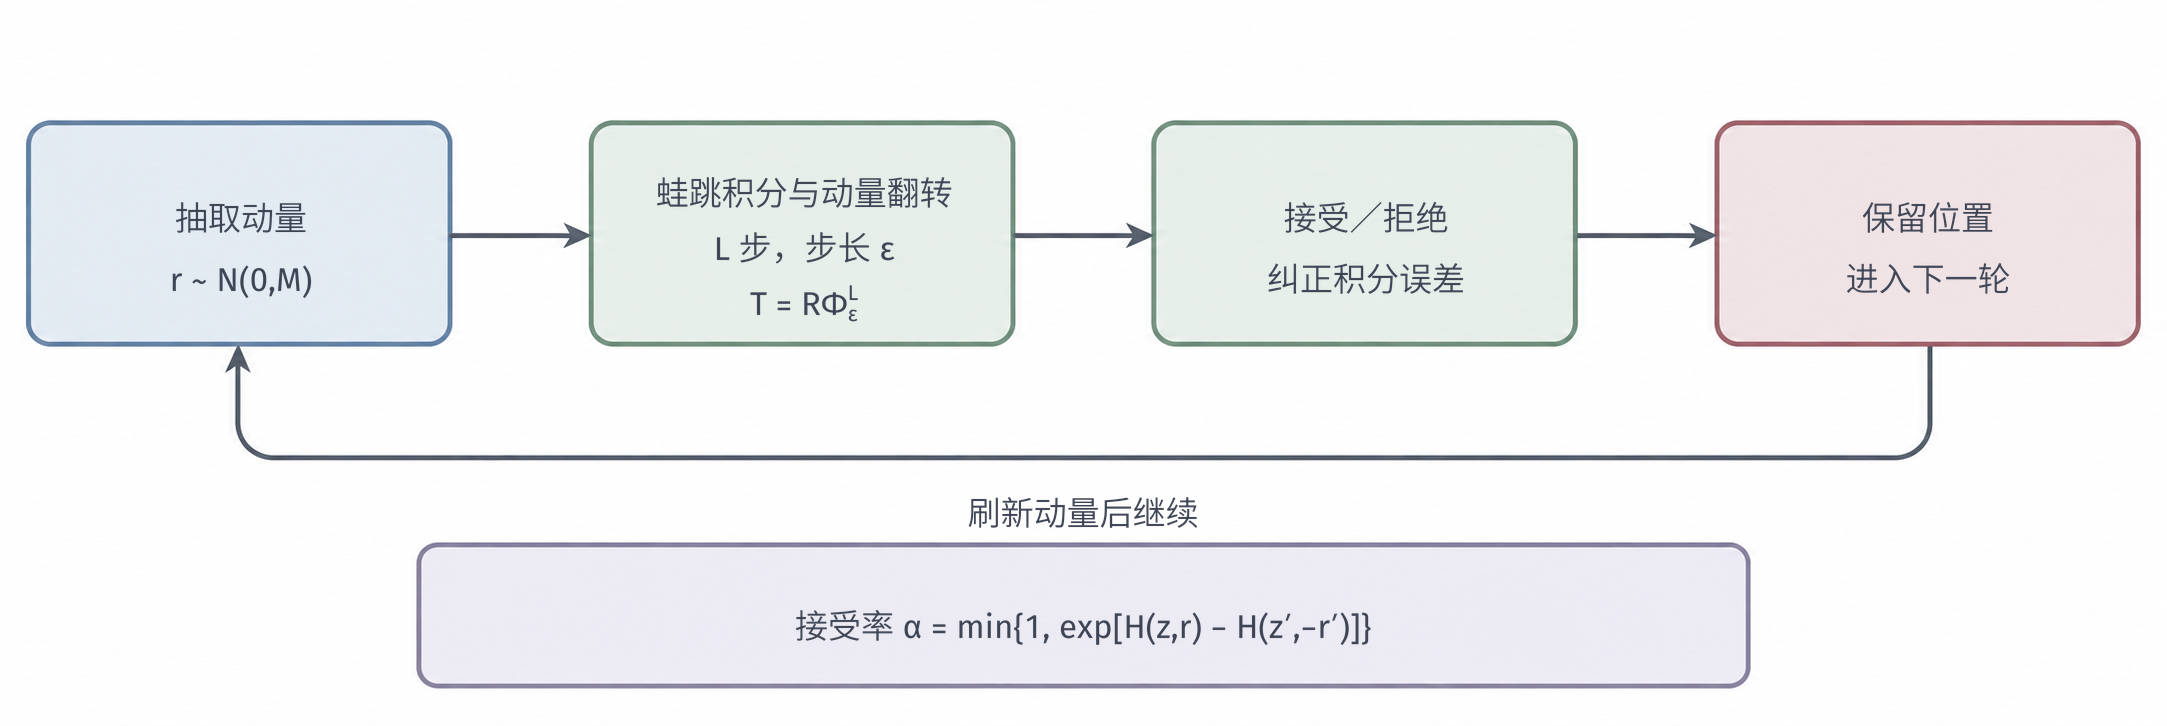
\includegraphics[width=169.000mm]{figures/09-probabilistic-graphical-models/02-inference/generated/pgm-sampling-hmc/figure.png}
  \par\medskip
  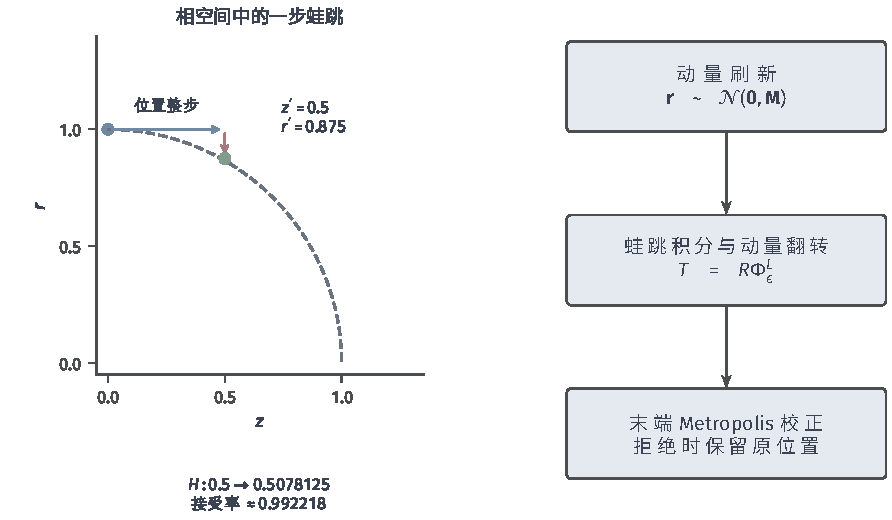
\includegraphics[width=142.118mm]{figures/09-probabilistic-graphical-models/02-inference/matplotlib/pgm-sampling-hmc/figure.pdf}
  \caption{HMC的更新流程与标准正态目标的一步数值计算。上方依次刷新动量、执行蛙跳并翻转末端动量、接受或拒绝提议、记录位置；$\bm z$是位置，$H$表示扩展状态的哈密顿量。下方的数值图由解析式生成：虚线圆弧属于$H=1/2$的精确轨迹，折线表示$\epsilon=0.5$的蛙跳整步与末端动量半步；初始动量半步因$z=0$不移动。动量翻转未画在相图上，接受率约为0.992218。}
  \label{fig:pgm-sampling-hmc}
\end{figure*}

步长$\epsilon$决定局部积分精度，轨迹长度$\tau=L\epsilon$决定一次提议运动多久。在足够光滑、数值稳定且$\tau$固定的条件下，蛙跳的全局状态误差为$O(\epsilon^2)$；在相应有界区域内，能量误差也可控制在这一阶。误差常数依赖曲率、维度和轨迹，采样误差还取决于链的探索。过大步长可能造成能量误差突然增大、非有限数值或拒绝；此类积分失败应拒绝并记录。过短轨迹探索不足，过长轨迹可能绕回原处，增加梯度计算却没有相应收益。

质量矩阵改变的是运动几何。为了看清它与目标尺度的关系，考虑高斯目标$\mathcal{N}(\bm{0},\bm{\Sigma})$，其中$\bm\Sigma$对称正定。此时$U(\bm z)=\tfrac12\bm z^{\top}\bm\Sigma^{-1}\bm z$加上常数，故$\nabla U(\bm z)=\bm\Sigma^{-1}\bm z$。由于$\bm M$固定，对位置方程再求一次导数，并代入动量方程，就得到
\[
  \frac{\mathrm{d}^2\bm{z}}{\mathrm{d}s^2}
     =\bm M^{-1}\frac{\mathrm d\bm r}{\mathrm ds}
     =-\bm{M}^{-1}\bm{\Sigma}^{-1}\bm{z}.
\]
按本章动量协方差等于$\bm M$的约定，取$\bm M=\bm\Sigma^{-1}$后，右侧变为$-\bm z$。每个坐标都满足$\mathrm d^2z_j/\mathrm ds^2=-z_j$，即频率为$1$的简谐运动；原来不同方向的快慢因而在人工时间下得到统一。软件中的“度量”和“逆质量”可能采用相反矩阵约定，使用时应先核对动量协方差与动能公式。固定矩阵补偿的是全局线性尺度；随位置变化的狭窄区域和多峰障碍需要其他几何或采样处理。通常在预热阶段调整尺度，正式保留样本时固定参数；任意依赖历史的持续调整不能直接套用上述齐次链证明。

若一次梯度求值成本为$C_{\nabla U}$，一轮HMC约需$O(L C_{\nabla U})$，另加动量生成和质量矩阵运算。对角矩阵的线性代数成本为$O(d)$每步，稠密矩阵通常为$O(d^2)$每步，并需预先分解。标准HMC不能直接更新离散变量；受约束连续变量常需先变换到无约束空间，并把变换的Jacobian加入密度。

计算出一条长轨迹也不保证位置移动有效。以标准正态和$M=1$的精确流为例，位置满足$z(s)=z(0)\cos s+r(0)\sin s$。若固定轨迹长度为$2\pi$，则不论本轮刷新出什么动量，末端位置都回到$z(0)$；精确积分的接受率虽为$1$，位置链却不移动。这就是固定长度与运动周期\term{共振}（resonance）妨碍遍历的一个最小例子。因此，积分误差控制之外仍需另外检查链的探索能力。

\section{序贯蒙特卡洛}
\label{sec:pgm-sampling-smc}

前面的MCMC针对“一个固定的后验分布”反复采样。但在很多实际问题里，观测是随时间一个接一个到来的（传感器持续上报、目标不断移动），目标分布每个时刻都在变；若每来一个观测就从头跑一条MCMC链，代价太高。自然的想法是让一群带权样本（粒子）随时间一起“向前走”，并在新观测到来时调整它们的权重。\term{序贯蒙特卡洛}（sequential Monte Carlo, SMC）复用上一阶段的样本及权重，逐步追踪一列目标分布。带权样本称为\term{粒子}（particle），每个粒子表示一个可能的潜在状态或状态历史。

为建立最小动态设定，令潜在状态为$\bm{z}_t$、观测为$\bm{x}_t$，真实时间$t=1,\ldots,T$写作下标。初始分布为$p(\bm{z}_1)$，转移分布为$p(\bm{z}_t\mid\bm{z}_{t-1})$，观测分布为$p(\bm{x}_t\mid\bm{z}_t)$。其联合分布分解为
\begin{equation}
  \begin{aligned}
    &p(\bm{z}_{1:T},\bm{x}_{1:T})\\
    &\qquad=p(\bm{z}_1)p(\bm{x}_1\mid\bm{z}_1)
       \prod_{t=2}^{T}
         p(\bm{z}_t\mid\bm{z}_{t-1})p(\bm{x}_t\mid\bm{z}_t).
  \end{aligned}
  \label{eq:pgm-sampling-state-space}
\end{equation}
这里假设给定上一潜状态后，更早状态不再影响当前状态；给定当前潜状态后，当前观测不再依赖其余变量。\term{滤波}（filtering）的目标是$p(\bm{z}_t\mid\bm{x}_{1:t})$，只利用截至当前的观测估计当前状态。若利用未来观测估计过去状态，则是平滑问题。本节只建立粒子计算所需的模型；第~\ref{sec:pgm-dynamic-common}节将从动态有向分解系统建立这些查询，第~\ref{sec:pgm-dynamic-continuous}节再比较何时可以用解析滤波代替粒子近似。

SMC不只适用于物理时间。一列$\gamma_\ell(\bm{z})=p(\bm{z})p(\bm{x}\mid\bm{z})^{\beta_\ell}$，其中$0=\beta_0<\cdots<\beta_L=1$，也可让粒子逐步从先验迁移到后验。这里的$\beta_\ell$是似然的指数，通常称为逆温度参数；指数从$0$增至$1$，表示逐步增强同一组观测对目标的影响，而不是增加新的观测。设各阶段归一化常数有限且为正，先验阶段按$\gamma_0=p(\bm z)$定义。对已有粒子，相邻阶段在其取值处的目标比为
\[
  \frac{\gamma_\ell(\bm z)}{\gamma_{\ell-1}(\bm z)}
    =p(\bm x\mid\bm z)^{\beta_\ell-\beta_{\ell-1}},
\]
其中比值只在前一阶段目标为正的位置计算；零似然位置在正指数阶段得到零权重。粒子据此更新权重，再按需要重采样，并进行保持当前归一化目标的MCMC移动。权重负责相邻目标的改变，MCMC核则在目标固定的当前阶段移动粒子。这里的$\ell$标记逆温度递增的算法阶段，与观测时间不同。本节以\term{粒子滤波}（particle filtering）为主，即用SMC近似式~\eqref{eq:pgm-sampling-state-space}的滤波分布。

\subsection{序贯重要性采样}
\label{sec:pgm-sampling-sis}

序贯重要性采样（SIS）就是把重要性采样改造成可随时间递推的形式：旧粒子继续保留，每步只需让它按状态转移“向前走一步”，再用新观测更新权重，而不必重算整条路径。路径后验涉及截至当前的全部潜状态，路径中的潜状态数量随时间增长。利用Markov分解，可以保留旧路径，只生成当前状态并更新权重。\term{序贯重要性采样}（sequential importance sampling, SIS）把路径提议写成
\[
  q_{1:t}(\bm{z}_{1:t}\mid\bm{x}_{1:t})
    =q_1(\bm{z}_1\mid\bm{x}_1)
      \prod_{s=2}^{t}
        q_s(\bm{z}_s\mid\bm{z}_{1:s-1},\bm{x}_{1:s}),
\]
其中每个$q_s$保持该阶段生成路径时所用的规则，使旧路径的提议密度仍由同一公共前缀表示。选择未归一化路径目标$\gamma_t=p(\bm{z}_{1:t},\bm{x}_{1:t})$。对$t\geq2$，新目标与新提议分别等于旧前缀乘上一个当前因子：
\[
  \begin{aligned}
    \gamma_t(\bm z_{1:t})
      &=\gamma_{t-1}(\bm z_{1:t-1})
          p(\bm z_t\mid\bm z_{t-1})p(\bm x_t\mid\bm z_t),\\
    q_{1:t}(\bm z_{1:t}\mid\bm x_{1:t})
      &=q_{1:t-1}(\bm z_{1:t-1}\mid\bm x_{1:t-1})
          q_t(\bm z_t\mid\bm z_{1:t-1},\bm x_{1:t}).
  \end{aligned}
\]
把两行相除，旧目标与旧提议的比值正是上一时刻的路径权重。因而不必重新计算整条路径的所有因子，只需保留旧权重，再乘新增目标因子与新增提议因子的比值。逐粒子写出这一关系，得到
\begin{equation}
  \begin{aligned}
    w_{1,i}&=
      \frac{p(\bm{z}_{1,i})p(\bm{x}_1\mid\bm{z}_{1,i})}
           {q_1(\bm{z}_{1,i}\mid\bm{x}_1)},\\
    w_{t,i}&=w_{t-1,i}
      \frac{p(\bm{z}_{t,i}\mid\bm{z}_{t-1,i})
            p(\bm{x}_t\mid\bm{z}_{t,i})}
           {q_t(\bm{z}_{t,i}\mid\bm{z}_{1:t-1,i},\bm{x}_{1:t})}.
  \end{aligned}
  \label{eq:pgm-sampling-sis-weight}
\end{equation}
下标$i=1,\ldots,n$标记粒子，$\bm{z}_{1:t,i}$是第$i$条路径。提议必须覆盖其对应的目标条件支撑集。权重的绝对尺度对归一化均值无影响，因此递推时可用上一时刻的归一化权重，再统一归一化当前权重。

路径后验中关于当前状态的查询，只使用$h(\bm z_t)$，与同一路径上更早坐标的具体记法无关。把路径经验分布对旧坐标边缘化，就相当于保留每条路径的权重和末端位置；这个操作不会把原来的不同权重自动变为等权。只保留路径末端，就得到滤波分布的经验近似
\begin{equation}
  \begin{aligned}
    \widehat p_t(\mathrm{d}\bm{z})
      &=\sum_{i=1}^{n}\bar w_{t,i}\delta_{\bm{z}_{t,i}}(\mathrm{d}\bm{z}),\\
    \widehat I_{t,h}&=\sum_{i=1}^{n}\bar w_{t,i}h(\bm{z}_{t,i}).
  \end{aligned}
  \label{eq:pgm-sampling-particle-measure}
\end{equation}
其中$\delta_{\bm{z}_{t,i}}$是把全部概率质量放在该粒子位置的点质量分布，不是连续密度曲线。若连续目标没有点质量，则有限粒子近似与它不可能在总变差距离下趋近。为看清这一点，取本次全部粒子位置组成的有限集合$B_n$：经验分布对$B_n$赋予概率$1$，无原子的目标却对$B_n$赋予概率$0$。按事件概率差的上确界定义，两者的总变差距离每次都是$1$。即使$n$增加，这个可随样本改变的有限集合仍能把两者区分开。因此，通常讨论的是适当测试函数$h$的积分是否收敛；这并不要求经验分布在总变差下收敛，也不把有限粒子解释为平滑的后验密度。

最简单的提议是模型转移$q_t=p(\bm{z}_t\mid\bm{z}_{t-1})$，此时新权重只是旧权重乘以当前观测似然。传播时尚未利用$\bm{x}_t$，所以新观测极具信息时，可能生成许多观测似然很低的候选。对预测似然有限且为正的父粒子，更有针对性的提议是
\begin{equation}
  \begin{aligned}
    q_t^\star(\bm{z}_t\mid\bm{z}_{t-1},\bm{x}_t)
      &=\frac{p(\bm{z}_t\mid\bm{z}_{t-1})
                p(\bm{x}_t\mid\bm{z}_t)}
              {p(\bm{x}_t\mid\bm{z}_{t-1})},\\
    p(\bm{x}_t\mid\bm{z}_{t-1})
      &=\int p(\bm{x}_t\mid\bm{z}_t)
             p(\bm{z}_t\mid\bm{z}_{t-1})\,\mathrm{d}\bm{z}_t.
  \end{aligned}
  \label{eq:pgm-sampling-optimal-proposal}
\end{equation}
它使式~\eqref{eq:pgm-sampling-sis-weight}中的增量变成只依赖父粒子的$p(\bm{x}_t\mid\bm{z}_{t-1,i})$，因而在给定父粒子的条件下，增量权重方差为零。这个“最优”只针对一步条件方差：不同父粒子的预测似然和旧权重仍可能不同，且$q_t^\star$本身可能难以计算或抽样。预测似然为零的父粒子对当前未归一化目标没有贡献，此时式中的条件提议无定义。

不重采样的SIS会把许多个增量相乘。若少数路径持续更符合观测，其权重会逐步占据总和的大部分，其他粒子虽仍占用计算，却几乎不影响答案。这称为\term{权重退化}（weight degeneracy）。在对数尺度上累加权重，并减去最大对数权重后再指数化，可以防止数值下溢，却不能消除这种真实的统计退化。

\subsection{粒子滤波与重采样}
\label{sec:pgm-sampling-particle-filter}

SIS有个随时间必然恶化的毛病：权重不断连乘，几步之后少数粒子会占据几乎全部权重，其余粒子形同虚设。一个自然的补救是“汰弱留强”——按权重概率性地复制好粒子、丢弃差粒子，使下一阶段的计算集中在更有希望的轨迹上。这就是重采样，加上它就成了粒子滤波。一个自然的补救是把下一轮计算资源更多地分给高权重粒子。\term{重采样}（resampling）按当前权重随机复制或淘汰粒子，把带权经验分布转成等权样本集合。若$N_i$为第$i$个原粒子的后代数，基本要求是
\begin{equation}
  \sum_i N_i=n,\qquad
  \mathbb{E}[N_i\mid\mathcal{F}_t]=n\bar w_{t,i},
  \label{eq:pgm-sampling-offspring}
\end{equation}
其中$\mathcal{F}_t$表示重采样前已有的全部粒子信息。由此，
\[
  \mathbb{E}\left[
     \left.\frac1n\sum_i N_i h(\bm{z}_{t,i})\right|\mathcal{F}_t
  \right]
    =\sum_i\bar w_{t,i}h(\bm{z}_{t,i}).
\]
重采样保持当前经验估计的条件期望。单次复制后的估计仍有随机波动，得到的后代也共享原粒子及路径信息。

三种常见方法都可以通过累积权重$C_j=\sum_{i=1}^{j}\bar w_{t,i}$实现。给定$u\in(0,1)$，取最小的$j$使$C_j\geq u$，便选中原粒子$j$。差异只在如何选择$n$个$u$，见表~\ref{tab:pgm-sampling-resampling}。

\begin{table}[htbp]
  \centering
  \begin{tabularx}{\linewidth}{@{}lXX@{}}
    \toprule
    方法 & 均匀数的构造 & 主要性质\\
    \midrule
    多项式 & $n$个独立的$u_i\sim\operatorname{Uniform}(0,1)$ & 后代数服从多项式分布，条件方差易分析\\
    分层 & 各区间$((i-1)/n,i/n)$独立抽一个$u_i$ & 每层均被使用，估计的条件方差不高于多项式法\\
    系统 & 抽一个$u\sim\operatorname{Uniform}(0,1/n)$，令$u_i=u+(i-1)/n$ & 只需一个随机偏移，结果受粒子排列影响\\
    \bottomrule
  \end{tabularx}
  \caption{固定粒子数的三种重采样。分层法的方差比较针对相同加权粒子集合和相同测试函数；系统法的方差还取决于排列与函数，需分别比较。}
  \label{tab:pgm-sampling-resampling}
\end{table}

\term{多项式重采样}（multinomial resampling）在给定$\mathcal{F}_t$后独立选取$n$个祖先，其均值估计的条件方差是
\begin{equation}
  \frac1n\left[
    \sum_i\bar w_{t,i}h(\bm{z}_{t,i})^2
      -\left(\sum_i\bar w_{t,i}h(\bm{z}_{t,i})\right)^2
  \right].
  \label{eq:pgm-sampling-resampling-variance}
\end{equation}
\term{分层重采样}（stratified resampling）用独立分层均匀数消除层间抽样次数的随机波动。其方差优势可以在同一组固定粒子和同一函数$h$上直接看出。令$a(u)$为累积权重规则选出的祖先索引，$g(u)=h(\bm z_{t,a(u)})$，并将$(0,1)$分成$n$个等长区间$J_j$。记均匀数落在第$j$层时，$g$的均值和方差分别为$\mu_j$和$s_j^2$，再令$\mu=n^{-1}\sum_j\mu_j$。给定重采样前的粒子后，多项式法的每个定位点先随机选层、再随机选层内位置，全方差公式给出
\[
  \begin{aligned}
    \operatorname{Var}(\widehat I_{\mathrm{mult}}\mid\mathcal F_t)
      &=\frac{1}{n^2}\sum_{j=1}^n s_j^2
          +\frac{1}{n^2}\sum_{j=1}^n(\mu_j-\mu)^2,\\
    \operatorname{Var}(\widehat I_{\mathrm{strat}}\mid\mathcal F_t)
      &=\frac{1}{n^2}\sum_{j=1}^n s_j^2.
  \end{aligned}
\]
这里两种$\widehat I$都表示复制后的等权函数均值。分层法在每层独立抽取一次，固定了各层的抽样次数，因而去掉了第二个非负的层间均值方差项。这会使条件方差不高于多项式法。\term{系统重采样}（systematic resampling）则共用一个随机偏移，容易实现。选中位置因共享偏移而相关，其方差比较需要考虑粒子排列和测试函数，不能直接继承分层法的上述独立求和。两者的比较和系统法反例见Douc等人的分析\scite{pgm-sampling-douc2005}

\term{自举粒子滤波}（bootstrap particle filter）将提议选为模型状态转移。下面依次传播粒子、按观测加权、输出本时刻估计，并在权重集中时重采样。也可以先重采样再传播，此时祖先提议及权重递推应与该顺序匹配。

\begin{algorithm}[带阈值重采样的自举粒子滤波]
  \label{alg:pgm-sampling-bootstrap}
  \begin{algorithmic}[1]
    \Require 状态空间模型、观测$\bm{x}_{1:T}$与时刻数$T\geq1$，查询函数$h$
    \Require 粒子数$n\geq1$，其中$n,T$为整数；阈值$\eta\in(0,1]$及重采样方案
    \Ensure 各时刻的滤波期望估计$\widehat I_{t,h}$
    \For{$t=1,\ldots,T$}
      \For{$i=1,\ldots,n$}
        \If{$t=1$}
          \State 抽取$\bm{z}_{1,i}\sim p(\bm{z}_1)$，置$v_i=1/n$
        \Else
          \State 抽取$\bm{z}_{t,i}\sim p(\bm{z}_t\mid\bm{z}_{t-1,i})$
          \State 置$v_i=\bar w_{t-1,i}$
        \EndIf
        \State $w_{t,i}\gets v_i p(\bm{x}_t\mid\bm{z}_{t,i})$
      \EndFor
      \State 若权重全零，报告本轮退化并停止；否则归一化为$\bar w_{t,i}$
      \State 输出$\widehat I_{t,h}=\sum_i\bar w_{t,i}h(\bm{z}_{t,i})$
      \If{$1/\sum_i\bar w_{t,i}^2<\eta n$且$t<T$}
        \State 按所选方案和$\bar w_{t,1:n}$抽取祖先索引$a_{t,1:n}$
        \State 同时复制旧$\bm{z}_{t,a_{t,i}}$为新$\bm{z}_{t,i}$，置$\bar w_{t,i}=1/n$
      \EndIf
    \EndFor
  \end{algorithmic}
\end{algorithm}

算法输入的$h$应是目标滤波分布下期望有定义的查询，$n$始终表示每轮粒子数，$T$表示输入观测的时刻数；它们不表示同一条MCMC链的运行长度。模型应能在生成粒子的位置给出非负有限的观测似然；若出现非有限值，应先报告模型或数值计算失败，不能把它作为有效权重继续归一化。所选重采样方案至少应满足式~\eqref{eq:pgm-sampling-offspring}的固定总后代数与条件后代均值。多项式、分层或系统方案均有前述构造，但其依赖结构和方差性质不同，不能只凭该均值条件就直接套用同一个中心极限定理。

阈值中的$1/\sum_i\bar w_{t,i}^2$衡量当前权重的集中程度，其含义和局限将在第~\ref{sec:pgm-sampling-diagnostics}节说明。重采样增加当前估计的随机性，多项式法的条件方差由式~\eqref{eq:pgm-sampling-resampling-variance}给出，所以算法先输出当前加权估计，再为后续传播重新分配粒子。权重全零时，归一化的粒子估计尚未定义，应检查提议覆盖、观测模型及粒子数，记录本轮退化。

\begin{example}[二状态设备的粒子滤波]
  \label{ex:pgm-sampling-filter}
  为单独观察时间递推，另设一个二状态教学模型。$Z_t\in\{0,1\}$表示当前故障状态，$X_t\in\{0,1\}$表示传感器读数。设
  \[
    \begin{aligned}
      p(Z_1=1)&=0.1,\\
      p(Z_t=1\mid Z_{t-1}=1)&=0.8,&
      p(Z_t=1\mid Z_{t-1}=0)&=0.1,\\
      p(X_t=1\mid Z_t=1)&=0.8,&
      p(X_t=1\mid Z_t=0)&=0.2.
    \end{aligned}
  \]
  收到$x_1=x_2=1$。精确滤波给出
  \[
    \begin{aligned}
      p(Z_1=1\mid x_1=1)&=\frac{0.1\times0.8}{0.1\times0.8+0.9\times0.2}
        =\frac4{13},\\
      p(Z_2=1\mid x_1=1)&=0.8\frac4{13}+0.1\frac9{13}
        =\frac{41}{130},\\
      p(Z_2=1\mid x_1=x_2=1)&=\frac{0.8\times41}{0.8\times41+0.2\times89}
        =\frac{164}{253}\approx0.648221.
    \end{aligned}
  \]
  假设上一轮已经得到等权粒子，传播到$t=2$的四个候选恰为$(0,1,1,0)$。其似然为$(0.2,0.8,0.8,0.2)$，归一化权重为$(0.1,0.4,0.4,0.1)$，故重采样前故障概率估计为$0.8$。

  用系统重采样，取偏移$u=0.05$，四个定位点为$0.05,0.30,0.55,0.80$；累积权重为$0.1,0.5,0.9,1$，因而祖先索引为$(1,2,3,3)$，新粒子为$(0,1,1,1)$。这次等权估计为$0.75$，不同于重采样前的$0.8$和精确答案。式~\eqref{eq:pgm-sampling-offspring}只保证对随机偏移再取期望后保持重采样前估计。
\end{example}

图~\ref{fig:pgm-sampling-resampling}展示第$3$个粒子被复制两次的过程。两个后代在复制瞬间相同，也共享过去的路径；后续随机转移可以分散当前位置，复制本身则无法恢复已经丢失的历史。\term{样本贫化}（sample impoverishment）指不同状态或祖先数量减少，它与权重集中对应不同的损失。状态噪声较小时，频繁重采样可能加重贫化；高维观测还可能使许多粒子的似然同时接近零。

\begin{figure}[htbp]
  \centering
  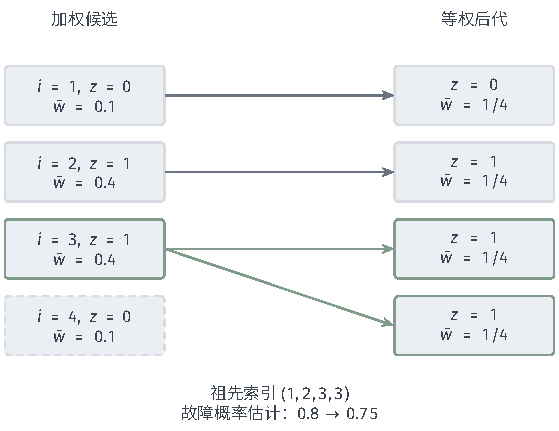
\includegraphics[width=94.650mm]{figures/09-probabilistic-graphical-models/02-inference/tikz/pgm-sampling-resampling/figure.pdf}
  \caption{二状态例子的系统重采样。左侧为四个带权候选，右侧为等权后代；连线标明复制来源。候选$4$没有后代，候选$3$被复制两次。后代等权，但状态及祖先多样性仍由复制来源决定。}
  \label{fig:pgm-sampling-resampling}
\end{figure}

若一次传播及似然计算成本分别为$C_{\mathrm{tr}},C_{\mathrm{obs}}$，一轮基础滤波成本约为$O(n(C_{\mathrm{tr}}+C_{\mathrm{obs}}))$，再加重采样成本。分层和系统法可沿累积权重单次扫描，在$O(n)$时间内完成；多项式法可用累积分布二分查找得到$O(n\log n)$实现，也有预处理后线性总成本的实现。只保存当前$d$维状态需$O(nd)$空间，保存所有粒子历史则随$T$增长。增加粒子数可改善固定时刻近似，长期平滑和高维滤波的效率还取决于路径与权重退化。

\subsection{Rao--Blackwell化粒子滤波}
\label{sec:pgm-sampling-rbpf}

粒子滤波对每个状态都要采样。若模型中一部分状态在给定其余状态时恰好有解析的条件分布（典型如离散模式下的连续状态服从线性高斯），就没必要也对它们采样——可以对这部分做精确Kalman递推，只对真正难处理的模式采样。这相当于在粒子滤波里再做一次Rao–Blackwell化。潜状态具有可解析的条件结构时，可以把随机计算集中到其余部分。\term{Rao--Blackwell化粒子滤波}（Rao--Blackwellized particle filtering, RBPF）只采样难以积分的状态部分，同时为每条粒子路径维护其余状态的条件分布。设$\bm{z}_t=(\bm{b}_t,\bm{u}_t)$，有
\begin{equation}
  \begin{aligned}
    &p(\bm{b}_{1:t},\bm{u}_t\mid\bm{x}_{1:t})\\
    &\qquad=p(\bm{b}_{1:t}\mid\bm{x}_{1:t})
        p(\bm{u}_t\mid\bm{b}_{1:t},\bm{x}_{1:t}).
  \end{aligned}
  \label{eq:pgm-sampling-rbpf-factor}
\end{equation}
若第二项可用有限维参数精确递推，则粒子只表示$\bm{b}_{1:t}$，每个粒子附带一份描述$\bm{u}_t$的解析状态。估计$h(\bm{b}_t,\bm{u}_t)$时，使用其条件期望
\[
  \widehat I_{t,h}^{\mathrm{RB}}
    =\sum_i\bar w_{t,i}
      \int h(\bm{b}_{t,i},\bm{u})
       p(\bm{u}\mid\bm{b}_{1:t,i},\bm{x}_{1:t})\,\mathrm{d}\bm{u}.
\]
查询中的条件分布已经使用当前观测$\bm x_t$，粒子加权却需要先计算看到该观测的概率。为区分这两个时刻，给定一条已扩展到$t$的模式路径，记
\[
  \begin{aligned}
    \pi_t^-(\bm u)
      &=p(\bm u_t=\bm u\mid\bm b_{1:t},\bm x_{1:t-1}),\\
    \ell_t(\bm b_{1:t})
      &=\int p(\bm x_t\mid\bm b_{1:t},\bm u)
                \pi_t^-(\bm u)\,\mathrm d\bm u.
  \end{aligned}
\]
这里$\pi_t^-$是当前观测进入之前的条件预测密度，$\ell_t$则是把连续状态积分掉后的预测观测密度。若$0<\ell_t<\infty$，看到$\bm x_t$后的条件密度才由Bayes公式给出：
\[
  \pi_t^+(\bm u)
    =\frac{p(\bm x_t\mid\bm b_{1:t},\bm u)\pi_t^-(\bm u)}
           {\ell_t(\bm b_{1:t})}.
\]
因此，查询积分使用$\pi_t^+$，权重计算使用$\pi_t^-$。把更新后的$\pi_t^+$再次当成预测分布来加权，会把同一次观测的影响重复算入。

模式路径本身也需要匹配提议。记模型在已有路径下的模式预测分布为
$a_t(\bm b_t)=p(\bm b_t\mid\bm b_{1:t-1},\bm x_{1:t-1})$，模式提议为$q_t^b(\bm b_t\mid\bm b_{1:t-1},\bm x_{1:t})$。对$t\geq2$，目标路径增加的因子为$a_t(\bm b_t)\ell_t(\bm b_{1:t})$，所以相应增量权重为
\[
  w_{t,i}\ \propto\ \bar w_{t-1,i}
    \frac{a_t(\bm b_{t,i})}
         {q_t^b(\bm b_{t,i}\mid\bm b_{1:t-1,i},\bm x_{1:t})}
    \ell_t(\bm b_{1:t,i}).
\]
比例常数在该轮粒子之间相同，重采样后的旧权重则按前述规则置为$1/n$。提议仍须覆盖有正目标贡献的模式；若模式按独立于连续状态的Markov链转移，则$a_t$简化为$p(\bm b_t\mid\bm b_{t-1})$。选择这一模式转移作为提议时，分式抵消，增量只剩积分预测似然；选择利用当前观测的其他模式提议时，分式必须保留。初始时刻同样使用模式先验与初始提议之比，并乘对应的初始积分观测密度。

典型例子是给定离散模式$b_t$后，连续状态服从线性高斯模型。每条模式路径维护高斯均值与协方差，通过Kalman递推完成条件滤波；模式仍用粒子表示。用标量的一步更新说明这一计算：给定某条模式路径及过去观测，连续状态预测分布为$U_t\sim\mathcal{N}(m^-,v^-)$，其中$v^->0$；观测满足$X_t=U_t+\varepsilon_t$，$\varepsilon_t\sim\mathcal{N}(0,\sigma_x^2)$，$\sigma_x^2>0$且噪声与$U_t$条件独立。预测观测是两个独立高斯量之和，故均值仍为$m^-$，方差为$v^-+\sigma_x^2$。这一步对未知$U_t$积分，也就是高斯卷积，得到用于模式权重的预测似然。

接着固定已经看到的$x_t$，更新连续状态。将先验预测密度与似然相乘，关于$u$的指数为
\[
  -\frac12\left[
       \left(\frac1{v^-}+\frac1{\sigma_x^2}\right)u^2
       -2\left(\frac{m^-}{v^-}+\frac{x_t}{\sigma_x^2}\right)u
       \right]+\text{与$u$无关的项}.
\]
因此，后验精度为$1/v_t=1/v^-+1/\sigma_x^2$，均值满足$m_t=v_t(m^-/v^-+x_t/\sigma_x^2)$。把分母通分，再把均值写成“预测均值加观测残差修正”的形式，便得到
\begin{equation}
  \begin{aligned}
    &p(x_t\mid b_{1:t},x_{1:t-1})
       =\mathcal{N}(x_t;m^-,v^-+\sigma_x^2),\\
    &k_t=\frac{v^-}{v^-+\sigma_x^2},\\
    &m_t=m^-+k_t(x_t-m^-),\qquad v_t=(1-k_t)v^-.
  \end{aligned}
  \label{eq:pgm-sampling-rbpf-gaussian}
\end{equation}
第一行对应观测前的积分预测似然，用于粒子权重；后两行给出观测后的条件高斯参数，用于查询和下一轮预测。$k_t$是标量Kalman增益，控制当前观测对条件均值的修正幅度：预测方差相对于观测噪声越大，当前残差得到的权重越大。上述卷积与配方承担不同计算，不能把观测后的条件高斯再次代入同一次预测似然。

假设两个等先验模式分别给出$U_t\sim\mathcal{N}(0,1)$和$\mathcal{N}(0,4)$，共同观测噪声方差$\sigma_x^2=1$，观测$x_t=1$。两模式的预测似然分别为$\mathcal{N}(1;0,2)\approx0.219696$和$\mathcal{N}(1;0,5)\approx0.161434$，归一化模式权重约为$0.576433,0.423567$。更新后的连续状态分别服从$\mathcal{N}(0.5,0.5)$和$\mathcal{N}(0.8,0.8)$，故混合均值约为$0.627070$。连续状态通过两个条件高斯表示，均值可直接积分，同时保留条件不确定性。从这些高斯额外抽样再估计均值，会引入额外的条件抽样波动。

RBPF利用可精确递推的条件分布减少随机性，但每个粒子需要存储协方差并进行矩阵运算，模式路径也可能退化。若用扩展Kalman等近似替代精确条件积分，结果中还包含条件滤波的近似误差。全方差公式解释相容条件化下的方差缩减；相同运行时间下的整体收益，则需比较粒子数、重采样和解析运算成本。Doucet等人的工作详细讨论了这一构造\scite{pgm-sampling-doucet2000}。

\section{算法分析}
\label{sec:pgm-sampling-analysis}

采样估计是否可信，需要同时说明目标、渐近规模与有限计算误差。渐近正确不代表有限时间内准确，不同机制的误差来源也不同：独立样本看权重和矩，MCMC看链的相关性与遍历性，粒子滤波还要看权重退化和祖先多样性。保持正确目标的核可能因探索缓慢而给出不可靠的有限估计，有有限样本偏差的比值估计也可能随样本数趋于一致。下面先逐一建立独立样本、加权样本、链与粒子的极限条件，再讨论能够从有限输出中直接检查的诊断量。

\subsection{一致性、偏差与方差}
\label{sec:pgm-sampling-consistency}

独立直接采样的条件最清楚。对固定查询$h$，独立同分布与$\mathbb{E}_p|h|<\infty$给出强一致性；$\mathbb{E}_p h^2<\infty$进一步给出式~\eqref{eq:pgm-sampling-iid-clt}的方差与中心极限定理。对于有界指示函数，这些矩条件自动成立。对于Cauchy等重尾分布，某些均值不存在，此时需要选择有定义的查询量。$n^{-1/2}$误差尺度也只描述随机计算误差，不包括模型失配。

重要性采样把这些矩条件移到了$q$下的加权函数。归一化目标的普通IS需要$r h$可积；有限方差与普通中心极限定理需要$\mathbb{E}_q(rh)^2<\infty$。SNIS的一致性条件见式~\eqref{eq:pgm-sampling-snis}之后。为了得到一个方便使用的SNIS中心极限定理，仍令候选独立来自固定$q$，要求目标支撑被覆盖、$0<Z_{\bm x}=\mathbb E_qw<\infty$，并进一步要求$\mathbb{E}_q w^2<\infty$和$\mathbb{E}_q(wh)^2<\infty$。

先把比值中同时变化的两部分写清。令$Y_i=w_i h(\bm z_i)$、$\bar Y_n=n^{-1}\sum_iY_i$与$\bar W_n=n^{-1}\sum_iw_i$，则$\widehat I_{h,n}^{\mathrm{SNIS}}=\bar Y_n/\bar W_n$，而$\mu_Y=\mathbb E_qY=Z_{\bm x}I_h$。记$\Delta_Y=\bar Y_n-\mu_Y$和$\Delta_W=\bar W_n-Z_{\bm x}$。联合中心极限定理使这两个偏差均为$O_{\mathbb P}(n^{-1/2})$；$\bar W_n$则依概率趋向严格正的$Z_{\bm x}$，所以分母为正的概率趋于$1$。有限样本的全零权重仍应按前文报告，不能输出归一化估计；讨论渐近分布时，可在这类事件上任意补定一个固定值，因为该事件概率趋零，不改变下面的分布极限。函数$f(a,b)=a/b$在该点对分子、分母的导数分别为$1/Z_{\bm x}$和$-I_h/Z_{\bm x}$，因而一阶展开为
\[
  \begin{aligned}
    \widehat I_{h,n}^{\mathrm{SNIS}}-I_h
      &=\frac{\Delta_Y-I_h\Delta_W}{Z_{\bm x}}
           +o_{\mathbb P}(n^{-1/2}),\\
    \Delta_Y-I_h\Delta_W
      &=\frac1n\sum_{i=1}^n w_i\bigl(h(\bm z_i)-I_h\bigr).
  \end{aligned}
\]
第二行利用$\mu_Y=Z_{\bm x}I_h$抵消常数项。它表明分母波动与分子波动共同形成中心化贡献，并且$\mathbb E_q[w(h-I_h)]=0$。对这个贡献应用独立样本中心极限定理，得到
\begin{equation}
  \begin{aligned}
    \sqrt n(\widehat I_{h,n}^{\mathrm{SNIS}}-I_h)
       &\xrightarrow{\mathrm{d}}\mathcal{N}(0,v_h^{\mathrm{IS}}),\\
    v_h^{\mathrm{IS}}
       &=\frac{\mathbb{E}_q[w^2(h-I_h)^2]}{Z_{\bm{x}}^2}.
  \end{aligned}
  \label{eq:pgm-sampling-snis-clt}
\end{equation}
关键的一阶随机量是$w(h-I_h)$，不是单独的$w$。这解释了为什么同一组权重对于不同查询可能具有不同精度。

SNIS的偏差也可由同一个比值展开看清，但这次需要控制取期望后的余项，只有一阶的依概率结论还不够。为简化书写，在以下展开中暂记$Z=Z_{\bm x}$。将$f(a,b)=a/b$在$(\mu_Y,Z)$处展开到二阶，得到
\[
  \begin{aligned}
    \widehat I_{h,n}^{\mathrm{SNIS}}-I_h
      &=\frac{\Delta_Y-I_h\Delta_W}{Z}\\
      &\quad-\frac{\Delta_Y\Delta_W}{Z^2}
         +\frac{I_h\Delta_W^2}{Z^2}+R_n,\\
    R_n&=\frac{\Delta_W^2(\Delta_Y-I_h\Delta_W)}
                  {Z^2\bar W_n}.
  \end{aligned}
\]
这里写出的$R_n$在$\bar W_n>0$时还是精确的余项表达。若在全零权重事件上将估计量补定为常数$c_0$，也应在该事件上把$R_n$定义为$c_0-I_h$。这是因为此时$\bar Y_n=\bar W_n=0$，已经显示的一阶和二阶项相互抵消，余项必须承接补定估计量与$I_h$的差。独立候选下，全零事件概率为$\mathbb P_q(w=0)^n$；由$\mathbb E_qw>0$可知$\mathbb P_q(w=0)<1$，所以这一补定对余项期望的贡献随$n$指数衰减，不改变下面的偏差阶。由于比值对分子线性，没有$\Delta_Y^2$项；分子与分母的交叉项带负号，反映分子固定时，分母增大会使比值减小。两个一次项的期望均为零，而独立候选给出
\[
  \mathbb E[\Delta_Y\Delta_W]
      =\frac{\operatorname{Cov}_q(wh,w)}n,\qquad
  \mathbb E[\Delta_W^2]=\frac{\operatorname{Var}_q(w)}n.
\]
在足够高阶矩和分母尾部控制使$\mathbb E R_n=o(n^{-1})$的条件下，对二阶展开取期望，便得到
\begin{equation}
  \mathbb{E}[\widehat I_{h,n}^{\mathrm{SNIS}}]-I_h
    =\frac{I_h\operatorname{Var}_q(w)-\operatorname{Cov}_q(wh,w)}
            {n Z_{\bm{x}}^2}+o(n^{-1}).
  \label{eq:pgm-sampling-snis-bias}
\end{equation}
例如$w\geq a>0$且$\mathbb{E}_q[w^4+|wh|^4]<\infty$，是控制分母和展开余项的一组较强充分条件。此时$\bar W_n\geq a$，两个样本均值偏差的二阶矩为$O(n^{-1})$、四阶矩为$O(n^{-2})$。将这些界代入$R_n$并使用Cauchy--Schwarz不等式，可得$\mathbb E|R_n|=O(n^{-3/2})=o(n^{-1})$。因此，常见的$O(n^{-1})$偏差来自交叉协方差与分母方差，而不是无条件的比值性质；这一阶数所需的余项和分母控制，比一致性所需的可积性与支持覆盖更强。

MCMC考察运行长度增长时的时间平均，其中样本通常相关。先说明强大数定律涵盖哪些起点。设固定的齐次转移核$K$在所声明的状态空间或闭合Harris类上正Harris常返，并保持概率分布$p$。对实值且满足$\mathbb E_p|h|<\infty$的$h$，从该类中的任意初始状态出发，时间平均都几乎必然收敛到$I_h$。这里“任意”限定在已经声明具有该性质的类内；仅知道某个核保持$p$，不足以把另一个封闭类中的起点也包括进来。非周期性另用于保证每一步的分布收敛；上述时间平均结论本身不要求非周期性。

若链从平稳分布启动，有限样本均值在期望存在时仍无偏，只是有相关性；从指定点启动时，有限预热用于减轻初值影响，剩余的初始化偏差还取决于核的混合速度。有限预热并不会把当前分布自动变成$p$，也不能替代一个结论所要求的起点条件。

MCMC中心极限定理还需额外条件。一组常用充分条件是\term{几何遍历性}（geometric ergodicity），即到平稳分布的距离按几何速率衰减，且允许系数依赖起点。具体地，在标准Borel状态空间上，设固定的齐次核$K$不可约、非周期且保持$p$，存在$0<a<1$及对$p$几乎处处起点有限的$C(\bm z)$，使
\[
  \lVert K^k(\bm z,\cdot)-p\rVert_{\mathrm{TV}}
    =\sup_B|K^k(\bm z,B)-p(B)|\leq C(\bm z)a^k.
\]
总变差距离在这里比较运行$k$步后的事件概率与目标事件概率，几何界控制两者相差的速率。标准Borel包括本章的欧氏空间及离散状态空间；这一可测性设定使常用条件分布和耦合论证能够适用。再要求某个$\delta>0$满足$\mathbb{E}_p|h|^{2+\delta}<\infty$，先从$\bm z^{(0)}\sim p$的平稳启动得到
\[
  \sqrt n(\widehat I_{h,n}-I_h)
     \xrightarrow{\mathrm{d}}\mathcal{N}(0,v_h^{\mathrm{MC}}).
\]
在上述一般几何遍历条件下，这个结论还可以扩展到$p$几乎处处的固定起点。这里允许排除$p$概率为零的异常起点。若进一步采用前面整类正Harris常返的设定，并保持非周期性，则该类中的每个起点都在总变差下收敛到$p$；将其与平稳链耦合，同一中心极限定理便可扩展到类内全部起点。这个扩展依据的是核在整类上的遍历性质，不是已经完成了有限预热。未被声明为该类成员的其他指定点，不能自动继承这个保证。

长期依赖的控制是推导正态误差分布所需的环节。再生方法把路径在特定随机返回时刻切成可以独立处理的完整区段，再控制初末不完整区段；Poisson方程方法则把中心化求和转为鞅差求和及可忽略的边界项，其中每个鞅差增量在给定过去信息时的条件均值为零。两者都需要证明相应矩和余项条件，不能只靠目标不变性得到正态误差。其他条件组合也可能建立中心极限定理，本章保留上述一组充分条件；更一般的证明以及从平稳启动扩展到$p$几乎处处固定起点的论证，见Roberts与Rosenthal的综述\scite{pgm-sampling-roberts2004}

SMC的样本数极限又不同：通常先固定一个有限时刻$t$，再令粒子数$n\to\infty$。为看清这一区别，可以考察一组较强而易检查的充分条件：初始粒子独立来自模型初始分布，传播使用正确的Markov转移；每个固定时刻的观测似然作为状态函数有正下界和有限上界；测试函数$h$有界；采用固定日程的多项式重采样。此时滤波积分估计一致，并满足适当的$\sqrt n$中心极限定理。一般提议需要相应的重要性权重矩条件，其他重采样方案和自适应日程还需要各自的方差与依赖条件，后代数条件无偏只是其中一项要求。

固定时刻一致性的证明思路是归纳。给定旧粒子后，新传播条件独立，因此对有界函数，传播抽样相对于其条件均值的方差为$O(1/n)$。条件均值是旧经验分布对转移后函数的积分，由归纳假设收敛。乘有界似然并除以远离零的归一化常数，仍保持收敛；多项式重采样再增加一个由式~\eqref{eq:pgm-sampling-resampling-variance}控制的$O(1/n)$条件方差。固定步数下反复使用这三个步骤便得到一致性。这是证明纲要，中心极限定理还需追踪每一代随机扰动如何传播，渐近方差包含历史各代贡献，而不只是当前粒子的样本方差\scite{pgm-sampling-chopin2004}

上述证明中的误差常数可以随$t$迅速增大。固定$n$让时间无限延长，与固定$t$让$n$趋向无穷，是不同的极限；要获得时间一致误差界，通常还需状态转移的遗忘或混合性质，以及适当的似然控制。归一化粒子滤波均值一般有有限$n$偏差。边缘似然却可以有无偏的粒子估计，因为它保留的是未归一化积分，而不是随机分母下的比值。

先把需要保存的尺度接回算法~\ref{alg:pgm-sampling-bootstrap}。记$g_t(\bm z)=p(\bm x_t\mid\bm z)$，传播后、归一化前的权重为$w_{t,i}=v_i g_t(\bm z_{t,i})$，其中$v_i$就是算法中的旧归一化权重，初始时为$1/n$。每轮归一化除掉的总和为
\begin{equation}
  \begin{aligned}
    \widehat c_t&=\sum_{i=1}^n v_i g_t(\bm z_{t,i}),\\
    \widehat Z_t&=\prod_{s=1}^t\widehat c_s,\qquad \widehat Z_0=1.
  \end{aligned}
  \label{eq:pgm-sampling-evidence-product}
\end{equation}
$\widehat c_t$近似预测观测密度$p(\bm x_t\mid\bm x_{1:t-1})$，$\widehat Z_t$近似边缘似然$p(\bm x_{1:t})$。初始时刻及上一轮已经重采样时$v_i=1/n$，因子是当前似然的粒子平均；上一轮未重采样时必须继续使用保留的非等权$v_i$。只保存归一化权重会丢掉这些总和。若为数值稳定对全部权重乘了共同尺度，计算$\widehat c_t$时还须还原该尺度，或在对数域保存对应的加数。

乘积的无偏性不能由“各因子分别无偏”推出，因为各轮使用的粒子相互依赖。可以直接对未归一化经验积分作条件递推。固定有限时刻和粒子数，先考虑初始独立模型采样、正确模型转移及每轮多项式重采样。观测似然非负有界、查询$h$有界，是使以下期望与积分均存在的一组充分条件。先约定：仅在截至当前每轮总权重都为正的存活事件上定义归一化经验积分；若某轮总权重为零，则直接把该运行的$\widehat Z_t$和$\Gamma_t^n(h)$定义为零，并在后续各轮维持为零，避免用零乘一个未定义的归一化积分。在存活分支上，令$\eta_t^n(h)$表示完成本轮可选重采样后的经验积分，$\Gamma_t^n(h)=\widehat Z_t\eta_t^n(h)$；未重采样时仍使用原来的加权积分。给定传播后的粒子，条件无偏的重采样使$\eta_t^n(h)$的条件均值等于$\sum_i\bar w_{t,i}h(\bm z_{t,i})$。因此，复制前的未归一化积分为
\[
  \widehat Z_{t-1}\sum_i v_i g_t(\bm z_{t,i})h(\bm z_{t,i}),
\]
复制后的$\Gamma_t^n(h)$在当前粒子信息下的条件期望与它相同；其中$\widehat c_t$恰好消去了归一化权重中的随机分母。对$t\geq2$，再对本轮传播取条件期望，有
\begin{equation}
  \begin{aligned}
    \mathbb E[\Gamma_t^n(h)\mid\mathcal F_{t-1}]
      &=\widehat Z_{t-1}\sum_i\bar w_{t-1,i}
          Q_t h(\bm z_{t-1,i}),\\
    Q_t h(\bm z)
      &=\int p(\bm z'\mid\bm z)g_t(\bm z')
                    h(\bm z')\,\mathrm d\bm z'.
  \end{aligned}
  \label{eq:pgm-sampling-evidence-recursion}
\end{equation}
这里$\mathcal F_{t-1}$包含上一轮重采样后的全部信息，$Q_t h$把一次状态转移、观测加权和当前查询合成一个旧状态的函数。含粒子状态与归一化权重的和式在对应存活分支上使用；若上一轮已经灭绝，递推两端都按零定义，无需再生成后续粒子。右侧正是$\Gamma_{t-1}^n(Q_t h)$。初始独立采样给出$\mathbb E\Gamma_1^n(h)=\int p(\bm z_1)g_1(\bm z_1)h(\bm z_1)\,\mathrm d\bm z_1$。据此逐轮取期望，便得到
\[
  \begin{aligned}
    \mathbb E\Gamma_t^n(h)
      &=\int h(\bm z_t)p(\bm z_t,\bm x_{1:t})\,\mathrm d\bm z_t,\\
    \mathbb E\widehat Z_t&=p(\bm x_{1:t}).
  \end{aligned}
\]
第二行取$h\equiv1$。它证明的是未归一化估计的无偏性；$\Gamma_t^n(h)/\widehat Z_t$仍有随机分母，因而不能据此判定滤波均值有限样本无偏。

若某轮权重全零，则当前滤波分布无法归一化，算法按原规则报告退化并停止。为了把证据估计定义在所有随机运行上，可将这种运行的$\widehat Z_t$及后续$\widehat Z_s$记为零，未归一化经验积分也记为零；此时不再要求定义对应的归一化滤波估计。零贡献必须保留在重复运行的平均中，不能丢弃失败运行、只对成功运行求平均后仍声称无偏。此前的一致性示例使用严格正下界，已经排除了全零事件；此处非负有界的设定则容许它出现。

按当前已有粒子信息决定是否重采样，例如算法中的权重ESS阈值，只要决策不使用未来随机量，且所选方案在该信息条件下仍保持后代均值，重采样或不重采样都保持同一个经验积分的条件期望，上述无偏递推仍可逐步应用。这个论证固定粒子数和要估计的时刻；任意改变粒子数、停止时刻、提议或目标的自适应规则需要重新核对权重与条件期望。即使某种自适应重采样保留了证据无偏性，其中心极限定理和方差公式也仍须满足该规则的额外条件。

\subsection{有效样本量与收敛诊断}
\label{sec:pgm-sampling-diagnostics}

估计精度既取决于样本数量，也取决于样本如何贡献以及如何相关。\term{有效样本量}（effective sample size, ESS）借独立样本的尺度描述这些影响。权重ESS衡量贡献集中，自相关ESS匹配具体查询的长期方差，两者需要分别解释。

先只考察归一化非负权重如何分配本批贡献。若恰有$m$个粒子各占$1/m$、其余为零，则平方权重和为$m(1/m)^2=1/m$，取倒数正好返回贡献相等的粒子数$m$。更一般地，按权重独立抽取两次索引，两次选中同一原粒子的概率为$\sum_i\bar w_i^2$。这一概率越大，权重越集中；其倒数用“等贡献粒子数”的尺度表示集中程度。由此引出常用的\term{权重有效样本量}（weight-based ESS）
\begin{equation}
  n_{\mathrm{eff}}^{w}
    =\frac{1}{\sum_i\bar w_i^2}
    =\frac{(\sum_i w_i)^2}{\sum_i w_i^2},
  \qquad 1\leq n_{\mathrm{eff}}^{w}\leq n.
  \label{eq:pgm-sampling-weight-ess}
\end{equation}
上下界来自非负性和Cauchy--Schwarz不等式：等权时等于$n$，一个权重占满总和时等于$1$。若候选确实独立来自固定$q$且$\mathbb{E}_q w^2<\infty$，大数定律还给出
\[
  \frac{n_{\mathrm{eff}}^{w}}{n}
    \longrightarrow
    \frac{(\mathbb{E}_q w)^2}{\mathbb{E}_q w^2}
    =\frac{1}{1+\operatorname{CV}_q(w)^2},
\]
其中$\operatorname{CV}_q(w)$为权重的标准差与均值之比。因此，权重ESS描述已抽到的贡献集中程度；对具体$h$的方差等价样本数，还需考虑函数值与权重的关系。真正的IS渐近方差还含有式~\eqref{eq:pgm-sampling-snis-clt}中的$(h-I_h)^2$。

表~\ref{tab:pgm-sampling-weight-example}中，$n_{\mathrm{eff}}^w=2.51^2/(0.01^2+0.9^2+0.9^2+0.7^2)\approx2.986$。这一数值只反映已抽到的权重，未访问的罕见状态仍需其他检查。粒子滤波例子重采样前的权重ESS为$1/(0.1^2+0.4^2+0.4^2+0.1^2)\approx2.941$，重采样后立即变成$4$；但图~\ref{fig:pgm-sampling-resampling}已经显示祖先反而减少。在SMC中，权重ESS主要帮助选择重采样时刻，滤波误差还需要考虑状态和祖先多样性。

MCMC常常所有样本等权，权重ESS因而为$n$。重复停留和缓慢移动带来的时间相关，需要通过样本均值的协方差分析。设链已平稳，$0<\sigma_h^2=\operatorname{Var}_p(h)<\infty$，令$\rho_h(\ell)$为$h(\bm{z}^{(k)})$与$h(\bm{z}^{(k+\ell)})$的相关系数。展开样本均值的协方差和，有
\begin{equation}
  \operatorname{Var}(\widehat I_{h,n})
    =\frac{\sigma_h^2}{n}
      \left[1+2\sum_{\ell=1}^{n-1}
          \left(1-\frac{\ell}{n}\right)\rho_h(\ell)\right].
  \label{eq:pgm-sampling-autocorrelation-variance}
\end{equation}
滞后$\ell$的样本对恰有$n-\ell$个，因而出现括号中的系数。若自相关绝对可和，定义\term{积分自相关时间}（integrated autocorrelation time）
\begin{equation}
  \tau_h=1+2\sum_{\ell=1}^{\infty}\rho_h(\ell),\qquad
  v_h^{\mathrm{MC}}=\sigma_h^2\tau_h,\qquad
  n_{\mathrm{eff},h}^{\mathrm{MC}}=\frac{n}{\tau_h}.
  \label{eq:pgm-sampling-mcmc-ess}
\end{equation}
这里假定$0<\tau_h<\infty$；还需前述中心极限定理条件，才能据此使用正态近似误差区间。$\tau_h$依赖函数$h$，故均值、尾概率和不同坐标通常有不同ESS；负相关还可能使$\tau_h<1$，此时ESS大于$n$，并不矛盾，因为它匹配的是估计方差而非独立点的实际数量。

例如平稳自回归序列的$\rho_h(\ell)=0.9^\ell$，则$\tau_h=1+2(0.9/0.1)=19$，$10000$次迭代对该查询只有约$526$个独立样本的渐近精度。对前述强相关高斯的Gibbs坐标，$\rho=0.99$给出的每轮相关系数为$0.9801$，对应$\tau_h=(1+0.9801)/(1-0.9801)\approx99.50$。两个例子将运行长度与该查询的渐近精度联系起来，高接受率仍可能伴随低有效样本量。简单地每隔若干步保留一个点虽然降低保留序列的相关性，也丢弃了已付费的计算；除非有存储或后续处理约束，稀疏保留不是改善采样效率的通用办法。

样本相关系数的高滞后估计噪声较大，不能把所有可计算滞后的样本相关系数直接相加。截断方法只累计到预先选定或按稳定规则选出的滞后，再检查截断位置改变时结论是否稳定；谱方差方法对样本自协方差施加随滞后衰减的窗权重，估计零频率处的长期波动尺度。批均值方法则把序列分成若干连续长批，使每批内部的相关都进入批均值，再用批间波动估计长期方差。

例如将$n$个保留的$h$值分为$a$个长为$b$的等长批，暂设$n=ab$，$a\geq2$。记第$j$批均值为$\bar H_j$、总均值为$\bar H$，可构造
\[
  \widehat v_h^{\mathrm{MC}}
    =\frac{b}{a-1}\sum_{j=1}^a(\bar H_j-\bar H)^2.
\]
若单批已经足够长，批均值的方差约为$v_h^{\mathrm{MC}}/b$，所以样本批方差乘以$b$对应所需的长期方差尺度。渐近使用时应让批长和批数都增长，并满足相应遍历与矩条件；前述中心极限定理本身不自动保证任意截断、窗宽或批长规则都一致。用$\sqrt{\widehat v_h^{\mathrm{MC}}/n}$报告具体查询的MCSE，可以把估计出的长期方差直接换回该查询的均值误差，而不是只报告一个全局ESS。

独立SNIS可以对式~\eqref{eq:pgm-sampling-snis-clt}作样本代入。在该式的覆盖与二阶矩条件下，以$\bar W_n$代替$Z_{\bm x}$、以$\widehat I_h$代替$I_h$，把期望代为样本平均，得到
\[
  \begin{aligned}
    \frac{\widehat v_h^{\mathrm{IS}}}{n}
       &=\frac{n^{-1}\sum_iw_i^2(h_i-\widehat I_h)^2}
               {n\bar W_n^2}\\
       &=\sum_i\bar w_i^2(h_i-\widehat I_h)^2,\\
    \widehat{\operatorname{MCSE}}(\widehat I_h)
       &=\left[\sum_i\bar w_i^2(h_i-\widehat I_h)^2\right]^{1/2},
       \qquad h_i=h(\bm z_i).
  \end{aligned}
\]
这里依赖候选独立与相应加权矩；若权重重尾到没有所需方差，代入一个有限数值不能恢复中心极限定理。共享祖先的粒子系统还包含额外依赖，不能直接把独立SNIS的式子当作其全部误差。SMC可通过多次独立运行整个粒子滤波比较估计波动，或采用专门的粒子方差估计。

单条链可能在一个局部区域内看起来很稳定。多链诊断从分散的有效初值运行若干条独立链，比较链内与链间变化。\term{$\widehat R$诊断}（R-hat diagnostic）用两种变化尺度之比发现不同链尚未探索相同分布的迹象。设共有$m\geq2$条链，每条保留$n\geq2$个函数值$h_{j,k}$，链均值为$\bar h_j=n^{-1}\sum_kh_{j,k}$，总体均值为$\bar h=m^{-1}\sum_j\bar h_j$，链内样本方差采用
\[
  s_j^2=\frac1{n-1}\sum_{k=1}^n(h_{j,k}-\bar h_j)^2.
\]
这里$n$表示每条链的保留长度，不是多条链合计长度。经典形式先计算链内平均方差$W$和按$n$放大后的链均值样本方差$B$，再构造
\begin{equation}
  \begin{aligned}
    W&=\frac1m\sum_{j=1}^{m}s_j^2,&
    B&=\frac{n}{m-1}\sum_{j=1}^{m}(\bar h_j-\bar h)^2,\\
    \widehat V&=\frac{n-1}{n}W+\frac{B}{n},&
    \widehat R&=\sqrt{\widehat V/W}.
  \end{aligned}
  \label{eq:pgm-sampling-rhat}
\end{equation}
$B/n$是各链均值之间的样本方差，$B$与$W$则都以单个函数值的方差为尺度。若各链已经近似探索同一分布且相关较弱，链均值方差约为单点方差除以$n$，所以$B$与$W$应大致相当；若链还停留在不同区域，链均值差异就可能使$B$明显增大。$\widehat V$将链内估计乘$(n-1)/n$，再补入链均值差异$B/n$，因而能够暴露只看链内波动遗漏的位置差异。样本相关与有限长度会影响这些估计，不能要求每次运行都恰有$\widehat R=1$。

该比值的通常解释要求$W>0$。所有链完全不动而使$W=0$时，比值无定义或缺少通常的尺度比较含义，应先检查链的移动，而不能将常数输出当成已经充分探索。

秩归一化的分裂诊断先把每条链的保留序列分成前后两半，并把各半段当成单独链。两半的位置差异因而能进入链间比较，帮助发现链内漂移；每半段仍需至少两个值，长度为奇数时可舍去中间一个值以保持两半等长。随后将全部半链样本合并排序，对并列值使用平均秩。若合计有$S$个值、某个值的秩为$r$，用$\Phi^{-1}((r-3/8)/(S+1/4))$将它映射为标准正态分位数，其中$\Phi$是标准正态分布函数。将变换后的值放回各自半链，按式~\eqref{eq:pgm-sampling-rhat}计算秩归一化的分裂$\widehat R$。这一变换保留排序信息，减轻原始重尾值对方差估计的影响。

位置相近的链仍可能具有不同尺度。为检查这一点，再计算每个原始样本到合并中位数的绝对偏差，对这些折叠值重新取秩、映射为正态分位数并计算分裂$\widehat R$。最终报告原始秩归一化分裂值与折叠后的值中的较大者，使位置或尺度差异中的任一种都能触发检查。

多链ESS还需要把每条链的时间相关与链间差异合在一起，不能简单相加各链单独报告的ESS。对当前要诊断的序列，仍以$m$表示半链数、$n$表示每条半链长度，并按式~\eqref{eq:pgm-sampling-rhat}重新计算$s_j^2,W,\widehat V$。沿第$j$条半链，用除数$n$计算各滞后的样本自协方差，再除以该链滞后零的自协方差，得到$\widehat\rho_{j,\ell}$。一种常用合并方式为
\begin{equation}
  \begin{aligned}
    \widehat\rho_\ell
      &=1-\frac{W-m^{-1}\sum_j s_j^2\widehat\rho_{j,\ell}}
                     {\widehat V},\\
    \widehat\tau&=1+2\sum_{\ell=1}^{L}\widehat\rho_\ell,\qquad
    \widehat n_{\mathrm{eff}}=\frac{mn}{\widehat\tau}.
  \end{aligned}
  \label{eq:pgm-sampling-multichain-ess}
\end{equation}
这里$L<n$是相关和的截断滞后，不是HMC的积分步数。若各链已经充分混合，使$\widehat V$与$W$接近，合并式近似对各链自相关按方差加权；若链均值差异使$\widehat V$增大，合并相关也随之增大，从而降低ESS。方差为零的单条半链不定义其相关系数，而把该链的自协方差贡献$s_j^2\widehat\rho_{j,\ell}$记为零；若合并方差也为零，则应报告退化并检查序列。

实际求和时，仍需避免高滞后噪声。常用做法将滞后$0,1$、$2,3$等相邻相关系数成对求和，保留从开头起连续为正的成对和；也可将后一个成对和限制为不大于前缀最小值，再整理为式~\eqref{eq:pgm-sampling-multichain-ess}的相关和。这给出初始正序列及其单调调整的截断规则。它们的理论性质与核的条件有关，不能把对任意短序列的数值输出当成已验证的长期方差；若估出的$\widehat\tau$非正或对截断极不稳定，应先检查运行长度和探索。总样本数在这里为$mn$，而不是任意一条半链的长度。

\term{主体ESS}（bulk ESS）根据秩变换后的序列，经上述合并与截断衡量主体区域的探索，却不直接给出原始均值的MCSE。\term{尾部ESS}（tail ESS）则针对两端分位的累计概率。令$\widehat q_\alpha$为合并样本的$\alpha$分位数，分别对$\alpha=0.05$和$0.95$构造沿链排列的指示序列$\mathbb{I}\{h_{j,k}\leq\widehat q_\alpha\}$，按同一多链合并与截断步骤分别计算两组序列的ESS，并取两个ESS的较小值。这些序列表示“落在分位阈值以下”的累计事件，不是“落在分位点附近某个小区间”的事件；上端累计事件也可取补集表示上尾，其相关结构相同。分位数误差还涉及分位处密度等条件，尾部ESS提供相应累计概率的探索诊断，不能代替所有尾部查询的精度分析。

原始均值和其他非线性查询的MCSE仍需按相应函数单独估计。常用的$\widehat R<1.01$是经验筛查标准，用于判断有限输出是否暴露出明显的多链差异；它不是已经收敛的证明。上述秩、折叠与尾部诊断的构造见Vehtari等人的论文\scite{pgm-sampling-vehtari2021}

有限输出的诊断可以共同检查多链轨迹、秩分布、查询函数的MCSE、主体和尾部ESS；HMC还需检查能量误差、积分失败与长时间拒绝。若所有链都局限于同一个模态，这些量仍可能正常。使用分散的有效初值，增加预算，检查模型几何，并与可解析特例或独立算法比较，有助于发现部分遗漏。诊断提供有限探索的证据，其范围仍受已访问区域限制。

\subsection{方法选择与计算边界}
\label{sec:pgm-sampling-choice}

采样器选择应从具体模型可计算的部件出发，而不是从方法的流行程度出发。若已有准确且廉价的直接采样器，独立平均通常最容易分析和并行；只有联合采样器而证据并不稀有时，拒绝采样能得到独立后验样本。若能够构造充分覆盖目标的提议，重要性采样便于并行且可估计归一化常数，但应优先检查权重尾部，而非仅拟合后验峰附近。

若只有未归一化密度及局部条件，MCMC可以避免全局提议的要求。满条件易抽样且相关适中时，Gibbs利用图结构获得低成本更新；强相关变量应考虑分块、折叠或重新参数化。连续密度可微时，HMC能用较贵的一次轨迹换取更远移动，但高维离散结构、多峰分离或复杂约束可能需要其他构造。若目标随新观测递推，粒子滤波直接复用过去计算；存在条件线性高斯部分时，RBPF可以把预算集中到真正需要采样的状态。

实际比较应固定查询与计算预算。一个每步便宜但高度相关的链，可能比一个每步较贵的链花更多时间才能达到同样MCSE。独立重要性采样虽可并行生成候选，若少数极端权重支配估计，多数候选对该查询的有效贡献仍然很小；独立MH则可能在到达高权重状态后长时间拒绝普通候选，表现为相关的重复停留。这两种损失分别通过贡献集中与链的时间依赖发生，不能只因都使用独立提议就混为同一种误差。因此应比较具体查询的MCSE随时间变化，或该查询的ESS每秒，并把预热、提议构造、梯度和解析积分计入成本。模型中的条件独立性帮助局部计算，却不保证后验中的统计相关很弱。

变分推断在可优化分布族中选择后验近似（第~\ref{chap:pgm-variational}章），采样则用随机经验表示估计后验积分。两者分别具有表达、求解和有限计算误差，表~\ref{tab:pgm-sampling-vi-comparison}在同一后验任务下比较这些因素。

\begin{table}[htbp]
  \centering
  \begin{tabularx}{\linewidth}{@{}lXX@{}}
    \toprule
    方面 & 采样近似 & 变分近似\\
    \midrule
    渐近目标 & 在相应覆盖、矩与遍历条件下，可逼近原后验积分 & 受分布族与目标函数限制，充分优化后仍可能有近似误差\\
    有限预算 & 有抽样波动，SNIS与非平稳MCMC等还可能有偏差 & 有分布族误差、优化误差，随机优化也有波动\\
    后验覆盖 & 漏模态、权重退化或慢混合会破坏有限样本覆盖 & 某些族与散度倾向集中于局部区域；覆盖行为取决于具体族与目标\\
    并行与规模 & 独立候选、多链和粒子可并行；单链有顺序依赖，重采样需同步 & 易利用小批量和摊销网络，但依赖相应模型与优化结构\\
    精度判断 & 查询相关的标准误与多种诊断并用 & 目标函数改善不等于所有后验查询都已准确\\
    \bottomrule
  \end{tabularx}
  \caption{在同一后验推断任务上比较采样与变分。渐近保证都有适用条件，有限预算下均需检查遗漏的后验结构。}
  \label{tab:pgm-sampling-vi-comparison}
\end{table}

两类方法还可以结合。拟合的变分分布可作为重要性采样或独立MH的提议，其支持覆盖与权重尾部决定后续校正和探索的效果。小规模、可高精度采样的问题则可提供变分误差的参照。具体方案需要在相同查询、计算预算和误差要求下比较。

\Needspace{8\baselineskip}
\section{本章小结}
\label{sec:pgm-sampling-summary}

采样推断用样本统计量估计后验概率和期望。独立候选通过目标生成、接受规则或权重匹配后验；Markov链通过保持目标的转移及充分探索计算时间平均；粒子系统通过传播、加权和后代分配追踪变化的目标。设备报警例说明，先验候选与后验候选回答不同的概率查询，相应的条件化或权重是得到所需答案的环节。

HMC以动量刷新、可逆保体积积分和Metropolis校正形成完整的后验更新。刷新改变轨迹方向和能量，可逆积分构造可配对的提议，末端校正处理离散能量误差。粒子滤波则以重采样把后续计算集中于高权重路径，但复制可能减少状态和祖先的多样性。两种方法均需将保持目标的构造与实际探索的效率分别检查。

误差分析与查询量和渐近条件对应。独立样本使用可积性与有限矩，重要性采样检查支持覆盖和加权矩，MCMC检查遍历及长期依赖，SMC通常先固定时间再增加粒子。权重ESS描述本批贡献集中，自相关ESS匹配具体函数的长期方差，多链诊断检查探索是否一致。可解析特例、查询相关的标准误和针对失效方式的诊断，为有限计算结果提供互补证据。

到这里，精确消元、变分优化和随机采样都在给定模型下回答查询。若局部概率本身还未知，后验期望便会进入参数更新，推断误差也可能影响学习结果。第~\ref{chap:pgm-parameter-learning}章接着说明这种依赖何时出现，以及观测完整且不含潜变量时为什么有些模型能免去内层推断。

\paragraph{扩展阅读}
Murphy的教材可用于扩展重要性采样和Markov链方法。进一步阅读时，可分别考察目标不变性、遍历条件、有限步混合以及查询相关的估计方差，理解接受率和轨迹形状为何只反映其中一部分性质\scite{pgm-murphy2012}。

